\documentclass[11pt]{beamer}

\title[Forman Profile --- Results]{Forman Profile Alignment: Results}
\author{Francesco Maria Guadagnuolo}
\date{\today}
\usetheme{Madrid}
\usecolortheme{whale}
\setbeamertemplate{navigation symbols}{}
\setbeamertemplate{headline}{}

\usepackage{graphicx}
\usepackage[english]{babel}
\usepackage{mathtools}
\usepackage{amssymb}
\usepackage{tikz}
\usepackage{pgfplots}
\pgfplotsset{compat=1.18}

\newcommand{\R}{\mathbb{R}}
\newcommand{\F}{\mathcal{F}}
\newcommand{\Ltil}{\widetilde{\Delta}_{\F}}
\newcommand{\norm}[1]{\left\|#1\right\|}

\begin{document}

\frame{\titlepage}

% ══════════════════════════════════════════════════════════════════════════════
%  METHODS
% ══════════════════════════════════════════════════════════════════════════════

\begin{frame}{Models and Configurations}
Two model families are studied, each run on 10 datasets with 10-fold cross-validation ($500$ epochs, early stopping at $200$):
\begin{itemize}
    \item \textbf{GeneralSheaf}: a neural sheaf learner maps each edge to an unconstrained $d\times d$ restriction map; the resulting sheaf Laplacian drives signal diffusion. Run with \texttt{save\_others=True}: the \emph{other Laplacian} (opposite normalisation, same maps) is also saved at every checkpoint.
    \item \textbf{JointSheafParams (Joint Diffusion)}: node signals and restriction maps are diffused jointly at each layer (\texttt{dual\_normalised=True}). Two initial-map modes:
    \begin{itemize}
        \item \textbf{Identity} (\texttt{learn\_first\_maps=False}): maps start as $I_d$; joint diffusion evolves them.
        \item \textbf{General} (\texttt{learn\_first\_maps=True}, \texttt{learnt\_map\_type=general}): a neural learner initialises maps before joint diffusion.
    \end{itemize}
    \item \textbf{Normalisation}: \texttt{normalised=True} applies symmetric normalisation $\widetilde{\Delta}_{\mathcal{F}} = D^{-1/2}\Delta_{\mathcal{F}} D^{-1/2}$; \texttt{normalised=False} uses the raw Laplacian. Every combination is run independently.
\end{itemize}
\end{frame}

\begin{frame}{Forman Profile Extraction}
\begin{itemize}
    \item \textbf{Bochner decomposition:} the sheaf Laplacian $\Delta_{\mathcal{F}}$ admits a block-diagonal curvature endomorphism $\mathrm{Ric}_{\mathcal{F}}$. Its per-node diagonal block $F_{u,u} \in \mathbb{R}^{d\times d}$ encodes how the learned maps deform the local geometry at node $u$.
    \item \textbf{Forman profile:} the $d$ eigenvalues of $F_{u,u}$ form the \emph{Forman profile} at node $u$. Stacking over all $n$ nodes gives an $(n,d)$ matrix of per-node curvature eigenvalues.
    \item \textbf{Checkpoint saving:} profiles are extracted and saved at epochs $\{0, 1, 5, 15, 50, 200\}$ \emph{and} at the best-validation-epoch (early stopping), for every fold and every layer. This yields a full training trajectory of the sheaf geometry.
    \item \textbf{Topological reference ($f_0^{\mathrm{top}}$):} the Forman profile of the \emph{augmented graph Laplacian} (topology-only, no learned maps) is saved once per fold and serves as the fixed geometric baseline.
\end{itemize}
\end{frame}

\begin{frame}{Alignment Metrics --- Normalised Laplacian (\texttt{normalised=True})}
For each eigenvalue channel $k=1,\dots,d$, per fold, per layer, and per checkpoint epoch, the following metrics compare the learned profile $f_k$ to the topological reference $f_k^{\mathrm{top}}$:
\begin{itemize}
    \item \textbf{Spearman $\rho$}: rank correlation between $f_k$ and $f_k^{\mathrm{top}}$ (node-level).
    \item \textbf{Pearson $r$}: linear correlation between $f_k$ and $f_k^{\mathrm{top}}$ (node-level).
    \item \textbf{Wasserstein $W_1$}: earth-mover distance between the empirical distributions of $f_k$ and $f_k^{\mathrm{top}}$.
    \item \textbf{RMSE}: $\ell_2$ distance between raw profile values and the topological reference.
    \item \textbf{NRMSE}: same as RMSE but after z-scoring both profiles (scale-invariant).
\end{itemize}
\medskip
All five metrics are averaged over eigenvalue channels $k$ and over folds, yielding one scalar per (checkpoint epoch, layer) cell. Visualised as heatmaps: rows = checkpoints, columns = layers.
\end{frame}

\begin{frame}{Alignment Metrics --- Unnormalised Laplacian (\texttt{normalised=False})}
When the Laplacian is unnormalised, eigenvalues are unbounded and the raw scale is not comparable to the normalised reference. A different metric set is therefore used:
\begin{itemize}
    \item \textbf{Wasserstein vs.\ topological} ($W_1(f_k, f_k^{\mathrm{top}})$): distribution distance to the topological profile.
    \item \textbf{Wasserstein vs.\ zero} ($W_1(f_k, \mathbf{0})$): distribution distance to the flat (all-zero) reference --- measures absolute spectral mass.
    \item \textbf{Pearson $r$ vs.\ topological}: linear correlation with $f_k^{\mathrm{top}}$ (shape alignment regardless of scale).
    \item \textbf{NRMSE vs.\ topological}: z-scored $\ell_2$ distance to $f_k^{\mathrm{top}}$ (scale-invariant divergence from topology).
    \item \textbf{RMSE vs.\ zero} ($\|f_k\|_2 / \sqrt{n}$): root-mean-square magnitude of the learned profile itself.
\end{itemize}
\medskip
This set captures both how far the profile drifts from topology \emph{and} how large the learned curvature values become in absolute terms.
\end{frame}

\begin{frame}{The \emph{Other Laplacian}: Isolating the Role of Normalisation}
For \textbf{GeneralSheaf} only, a parallel Laplacian is computed at every checkpoint using the \emph{same learned restriction maps} but the \emph{opposite normalisation}:
\begin{itemize}
    \item If the model was trained with \texttt{normalised=True}, the other Laplacian is $\Delta_{\mathcal{F}}$ (unnormalised). Its Forman profile is saved in \texttt{other\_Laplacian/}.
    \item If trained with \texttt{normalised=False}, the other Laplacian is $\widetilde{\Delta}_{\mathcal{F}} = D^{-1/2}\Delta_{\mathcal{F}} D^{-1/2}$ (normalised).
\end{itemize}
This allows four analysis modes (XOR logic on content type):
\begin{enumerate}
    \item Norm=True primary: normalised profile vs.\ normalised topology.
    \item Norm=False primary: unnormalised profile vs.\ topological reference.
    \item \texttt{--use\_other} from Norm=True run: unnormalised profile (same maps!) vs.\ topological reference.
    \item \texttt{--use\_other} from Norm=False run: normalised profile (same maps!) vs.\ topological reference.
\end{enumerate}
Modes 1 \& 4 both have normalised content; modes 2 \& 3 both have unnormalised content and use the unnormalised metric set.
\end{frame}

\begin{frame}{Cross-Comparison: Motivation}
The primary runs and the \emph{other Laplacian} give us \textbf{four Forman profiles} for each dataset, two normalised and two unnormalised:

\medskip
\begin{center}
\renewcommand{\arraystretch}{1.4}
\begin{tabular}{l|cc}
 & \textbf{Normalised} $\widetilde{\Delta}_\mathcal{F}$ & \textbf{Unnormalised} $\Delta_\mathcal{F}$ \\
\hline
Maps trained with \texttt{norm=True}  & \textit{primary run}         & \texttt{other\_Laplacian} \\
Maps trained with \texttt{norm=False} & \texttt{other\_Laplacian}    & \textit{primary run}      \\
\end{tabular}
\end{center}

\medskip
\textbf{Key idea:} by comparing entries \emph{within the same column}, the normalisation (and hence spectral scaling) is \emph{identical} between the two profiles. The \emph{only} difference is whether the restriction maps were trained with or without normalisation.

\medskip
This isolates a precise question: \emph{does the training objective (normalised vs.\ unnormalised loss) push the learned maps toward a geometrically different sheaf, even when we evaluate both under the same Laplacian normalisation?}
\end{frame}

\begin{frame}{Cross-Comparison: The Two Directions}
\begin{itemize}
    \item \textbf{Direction A} (left column, both normalised):
    \begin{itemize}
        \item Profile 1: primary run with \texttt{norm=True} $\;\to\;$ $\widetilde{\Delta}_\mathcal{F}$ from maps trained normalised.
        \item Profile 2: \texttt{other\_Laplacian} of \texttt{norm=False} run $\;\to\;$ $\widetilde{\Delta}_\mathcal{F}$ from maps trained unnormalised.
        \item Both are \textbf{normalised Laplacians}; only the training regime differs.
    \end{itemize}
    \medskip
    \item \textbf{Direction B} (right column, both unnormalised):
    \begin{itemize}
        \item Profile 1: primary run with \texttt{norm=False} $\;\to\;$ $\Delta_\mathcal{F}$ from maps trained unnormalised.
        \item Profile 2: \texttt{other\_Laplacian} of \texttt{norm=True} run $\;\to\;$ $\Delta_\mathcal{F}$ from maps trained normalised.
        \item Both are \textbf{unnormalised Laplacians}; only the training regime differs.
    \end{itemize}
\end{itemize}
\medskip
\textbf{Metrics:} Spearman $\rho$, Pearson $r$, Wasserstein $W_1$, RMSE, NRMSE --- computed \emph{between the two learned profiles} (not against a topological baseline). Aggregated over folds and eigenvalue channels; displayed as heatmaps (rows = checkpoint epochs, columns = layers).
\end{frame}

% ══════════════════════════════════════════════════════════════════════════════
%  SECTION 1 — GeneralSheaf, normalised = True
% ══════════════════════════════════════════════════════════════════════════════

\begin{frame}{}
\centering
\Huge\textbf{GeneralSheaf}\\[6pt]
\Large Normalised Laplacian (\texttt{normalised=True})
\end{frame}

\begin{frame}{Amazon Ratings --- GeneralSheaf, $d=5$, $L=5$, Norm=True}
\begin{figure}
    \centering
    
\includegraphics[width=\linewidth]{heatmaps/GeneralSheaf/normalised_true/amazon_ratings_GeneralSheaf_d5_5L_Norm_True_heatmap.pdf}
\end{figure}
\end{frame}

\begin{frame}{Citeseer --- GeneralSheaf, $d=5$, $L=4$, Norm=True}
\begin{figure}
    \centering
    
\includegraphics[width=\linewidth]{heatmaps/GeneralSheaf/normalised_true/citeseer_GeneralSheaf_d5_4L_Norm_True_heatmap.pdf}
\end{figure}
\end{frame}

\begin{frame}{Cora --- GeneralSheaf, $d=3$, $L=3$, Norm=True}
\begin{figure}
    \centering
    
\includegraphics[width=\linewidth]{heatmaps/GeneralSheaf/normalised_true/cora_GeneralSheaf_d3_3L_Norm_True_heatmap.pdf}
\end{figure}
\end{frame}

\begin{frame}{Cora --- GeneralSheaf, $d=5$, $L=3$, Norm=True}
\begin{figure}
    \centering
    
\includegraphics[width=\linewidth]{heatmaps/GeneralSheaf/normalised_true/cora_GeneralSheaf_d5_3L_Norm_True_heatmap.pdf}
\end{figure}
\end{frame}

\begin{frame}{Cornell --- GeneralSheaf, $d=2$, $L=2$, Norm=True}
\begin{figure}
    \centering
    
\includegraphics[width=\linewidth]{heatmaps/GeneralSheaf/normalised_true/cornell_GeneralSheaf_d2_2L_Norm_True_heatmap.pdf}
\end{figure}
\end{frame}

\begin{frame}{Minesweeper --- GeneralSheaf, $d=5$, $L=6$, Norm=True}
\begin{figure}
    \centering
    
\includegraphics[width=\linewidth]{heatmaps/GeneralSheaf/normalised_true/minesweeper_GeneralSheaf_d5_6L_Norm_True_heatmap.pdf}
\end{figure}
\end{frame}

\begin{frame}{Pubmed --- GeneralSheaf, $d=5$, $L=4$, Norm=True}
\begin{figure}
    \centering
    
\includegraphics[width=\linewidth]{heatmaps/GeneralSheaf/normalised_true/pubmed_GeneralSheaf_d5_4L_Norm_True_heatmap.pdf}
\end{figure}
\end{frame}

\begin{frame}{Questions --- GeneralSheaf, $d=5$, $L=4$, Norm=True}
\begin{figure}
    \centering
    
\includegraphics[width=\linewidth]{heatmaps/GeneralSheaf/normalised_true/questions_GeneralSheaf_d5_4L_Norm_True_heatmap.pdf}
\end{figure}
\end{frame}

\begin{frame}{Roman Empire --- GeneralSheaf, $d=5$, $L=5$, Norm=True}
\begin{figure}
    \centering
    
\includegraphics[width=\linewidth]{heatmaps/GeneralSheaf/normalised_true/roman_empire_GeneralSheaf_d5_5L_Norm_True_heatmap.pdf}
\end{figure}
\end{frame}

\begin{frame}{Tolokers --- GeneralSheaf, $d=3$, $L=4$, Norm=True}
\begin{figure}
    \centering
    
\includegraphics[width=\linewidth]{heatmaps/GeneralSheaf/normalised_true/tolokers_GeneralSheaf_d3_4L_Norm_True_heatmap.pdf}
\end{figure}
\end{frame}

\begin{frame}{Wisconsin --- GeneralSheaf, $d=2$, $L=2$, Norm=True}
\begin{figure}
    \centering
    
\includegraphics[width=\linewidth]{heatmaps/GeneralSheaf/normalised_true/wisconsin_GeneralSheaf_d2_2L_Norm_True_heatmap.pdf}
\end{figure}
\end{frame}

% ══════════════════════════════════════════════════════════════════════════════
%  SECTION 2 — GeneralSheaf, normalised = False
% ══════════════════════════════════════════════════════════════════════════════

\begin{frame}{}
\centering
\Huge\textbf{GeneralSheaf}\\[6pt]
\Large Unnormalised Laplacian (\texttt{normalised=False})
\end{frame}

\begin{frame}{Amazon Ratings --- GeneralSheaf, $d=5$, $L=5$, Norm=False}
\begin{figure}
    \centering
    
\includegraphics[width=\linewidth]{heatmaps/GeneralSheaf/normalised_false/amazon_ratings_GeneralSheaf_d5_5L_Norm_False_heatmap.pdf}
\end{figure}
\end{frame}

\begin{frame}{Citeseer --- GeneralSheaf, $d=5$, $L=4$, Norm=False}
\begin{figure}
    \centering
    
\includegraphics[width=\linewidth]{heatmaps/GeneralSheaf/normalised_false/citeseer_GeneralSheaf_d5_4L_Norm_False_heatmap.pdf}
\end{figure}
\end{frame}

\begin{frame}{Cora --- GeneralSheaf, $d=3$, $L=3$, Norm=False}
\begin{figure}
    \centering
    
\includegraphics[width=\linewidth]{heatmaps/GeneralSheaf/normalised_false/cora_GeneralSheaf_d3_3L_Norm_False_heatmap.pdf}
\end{figure}
\end{frame}

\begin{frame}{Cora --- GeneralSheaf, $d=5$, $L=3$, Norm=False}
\begin{figure}
    \centering
    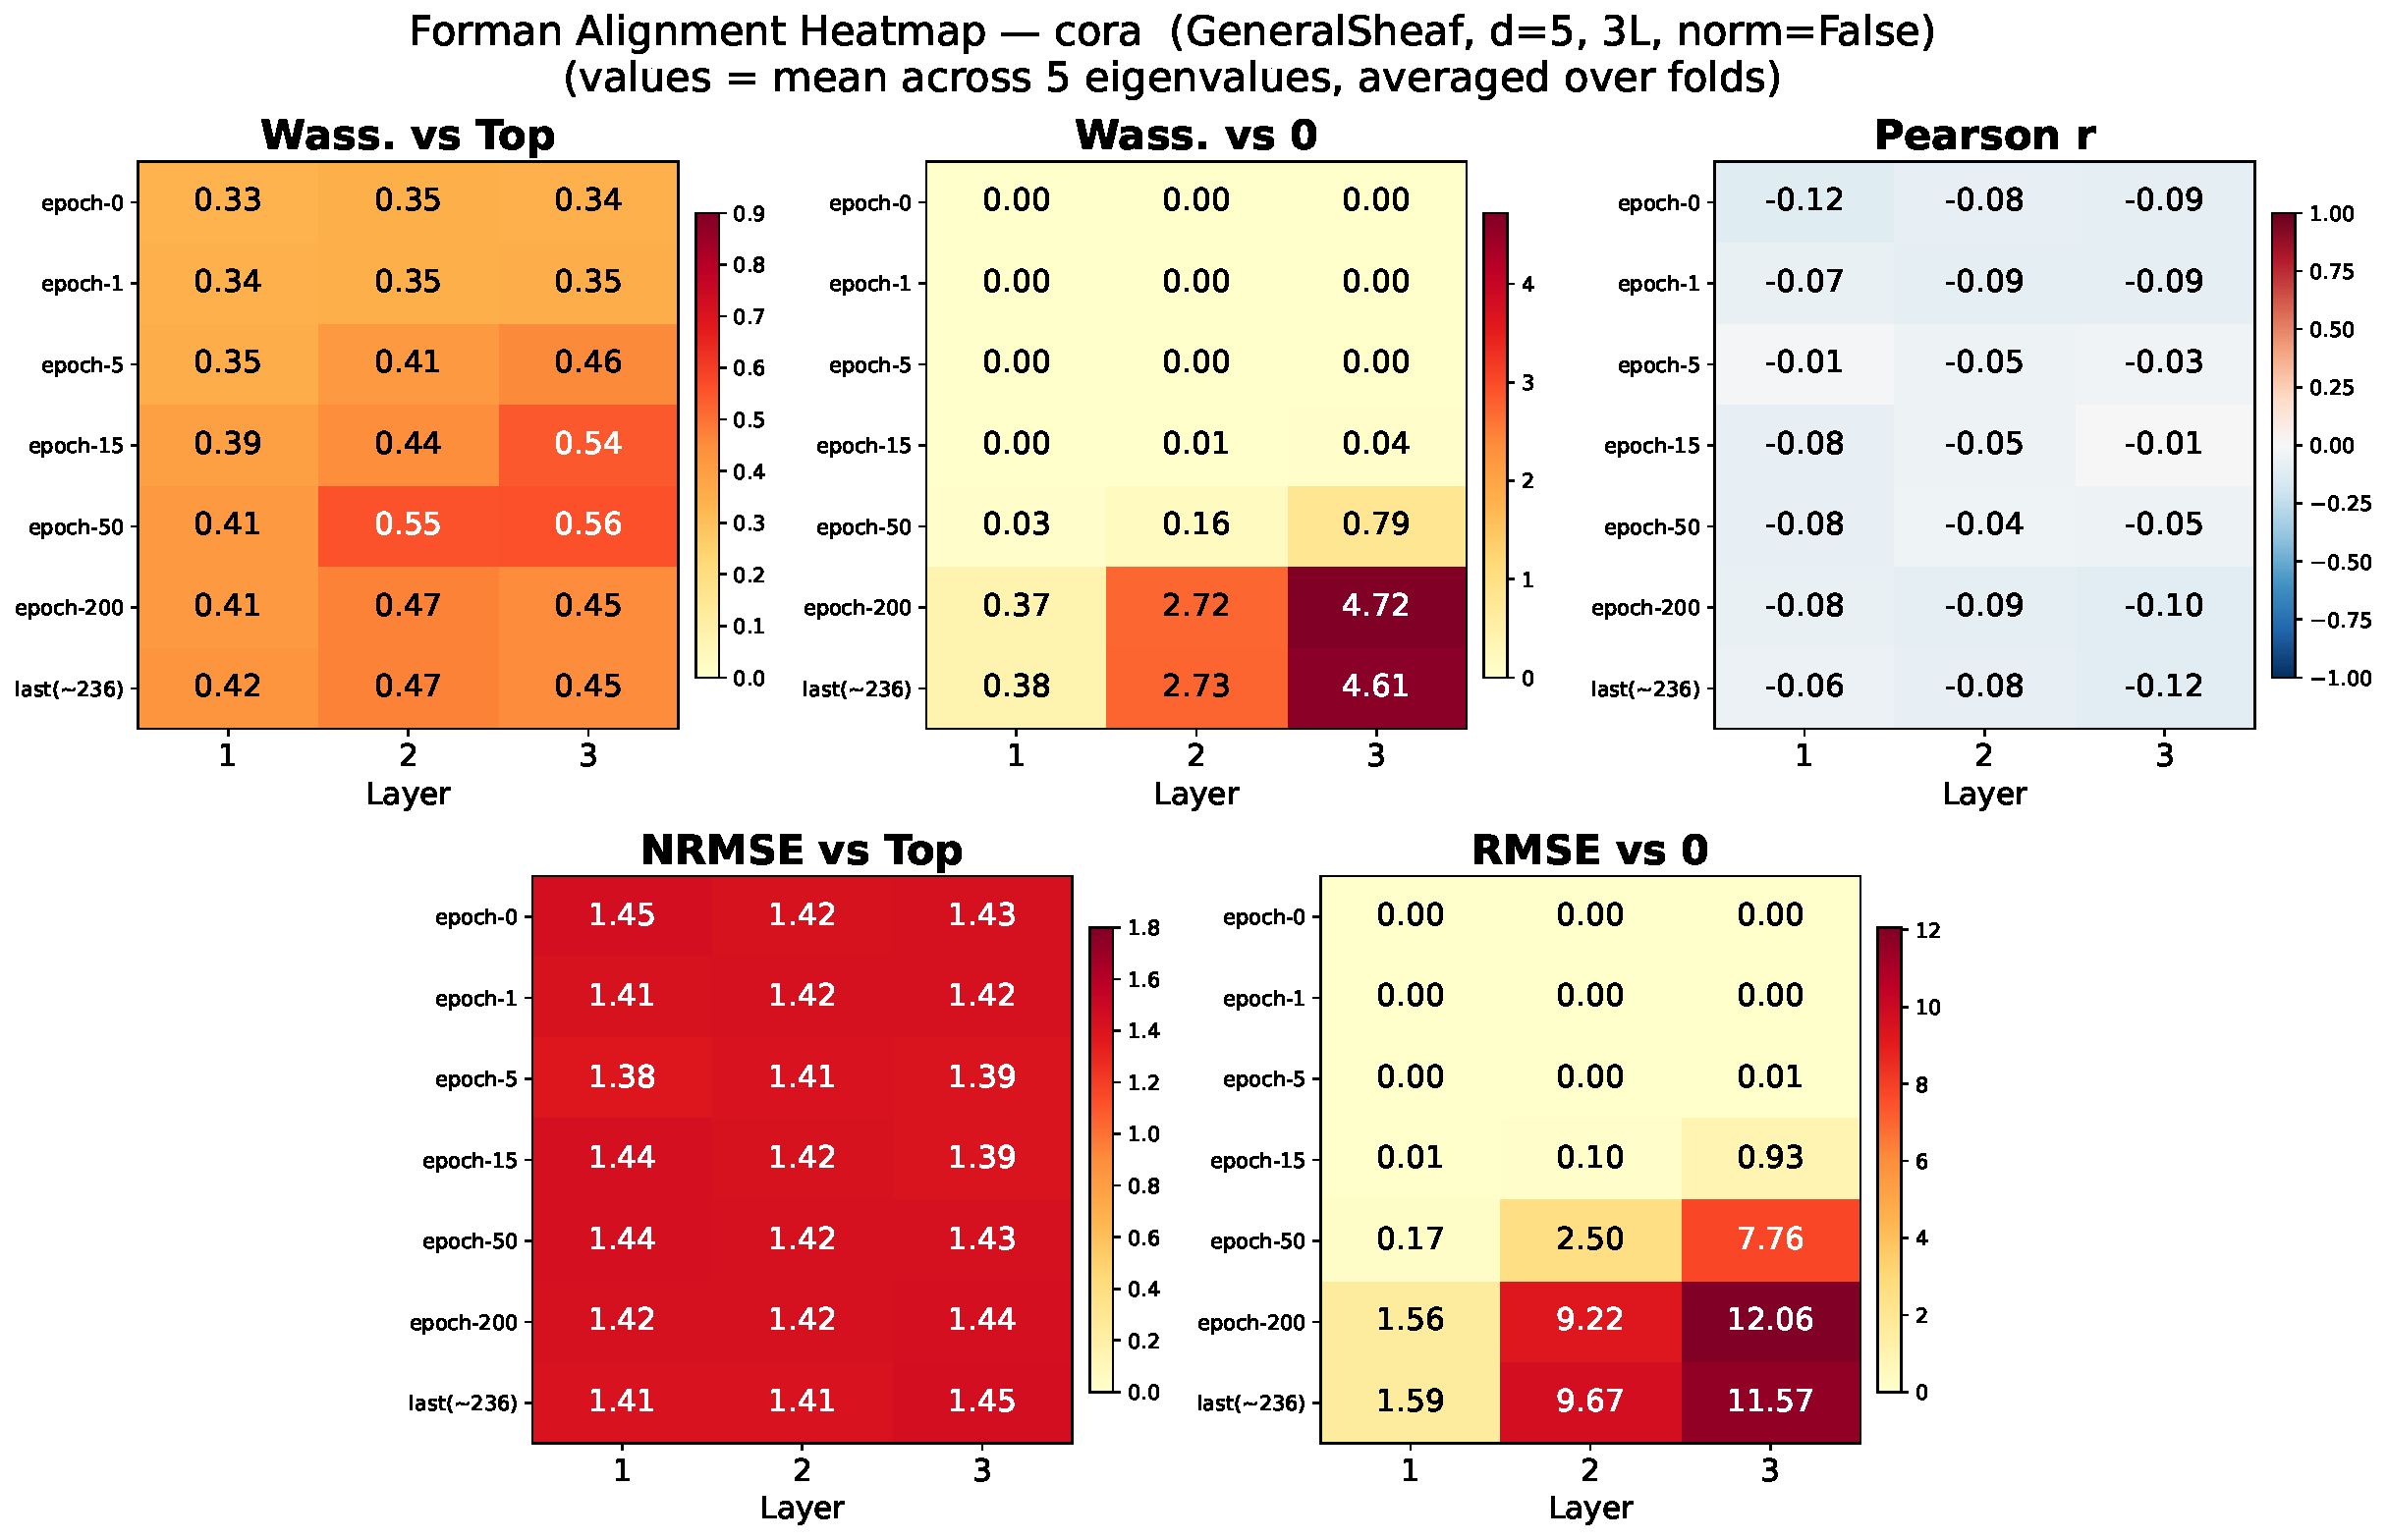
\includegraphics[width=\linewidth]{heatmaps/GeneralSheaf/normalised_false/cora_GeneralSheaf_d5_3L_Norm_False_heatmap.pdf}
\end{figure}
\end{frame}

\begin{frame}{Cornell --- GeneralSheaf, $d=2$, $L=2$, Norm=False}
\begin{figure}
    \centering
    
\includegraphics[width=\linewidth]{heatmaps/GeneralSheaf/normalised_false/cornell_GeneralSheaf_d2_2L_Norm_False_heatmap.pdf}
\end{figure}
\end{frame}

\begin{frame}{Minesweeper --- GeneralSheaf, $d=5$, $L=6$, Norm=False}
\begin{figure}
    \centering
    
\includegraphics[width=\linewidth]{heatmaps/GeneralSheaf/normalised_false/minesweeper_GeneralSheaf_d5_6L_Norm_False_heatmap.pdf}
\end{figure}
\end{frame}

\begin{frame}{Pubmed --- GeneralSheaf, $d=5$, $L=4$, Norm=False}
\begin{figure}
    \centering
    
\includegraphics[width=\linewidth]{heatmaps/GeneralSheaf/normalised_false/pubmed_GeneralSheaf_d5_4L_Norm_False_heatmap.pdf}
\end{figure}
\end{frame}

\begin{frame}{Questions --- GeneralSheaf, $d=5$, $L=4$, Norm=False}
\begin{figure}
    \centering
    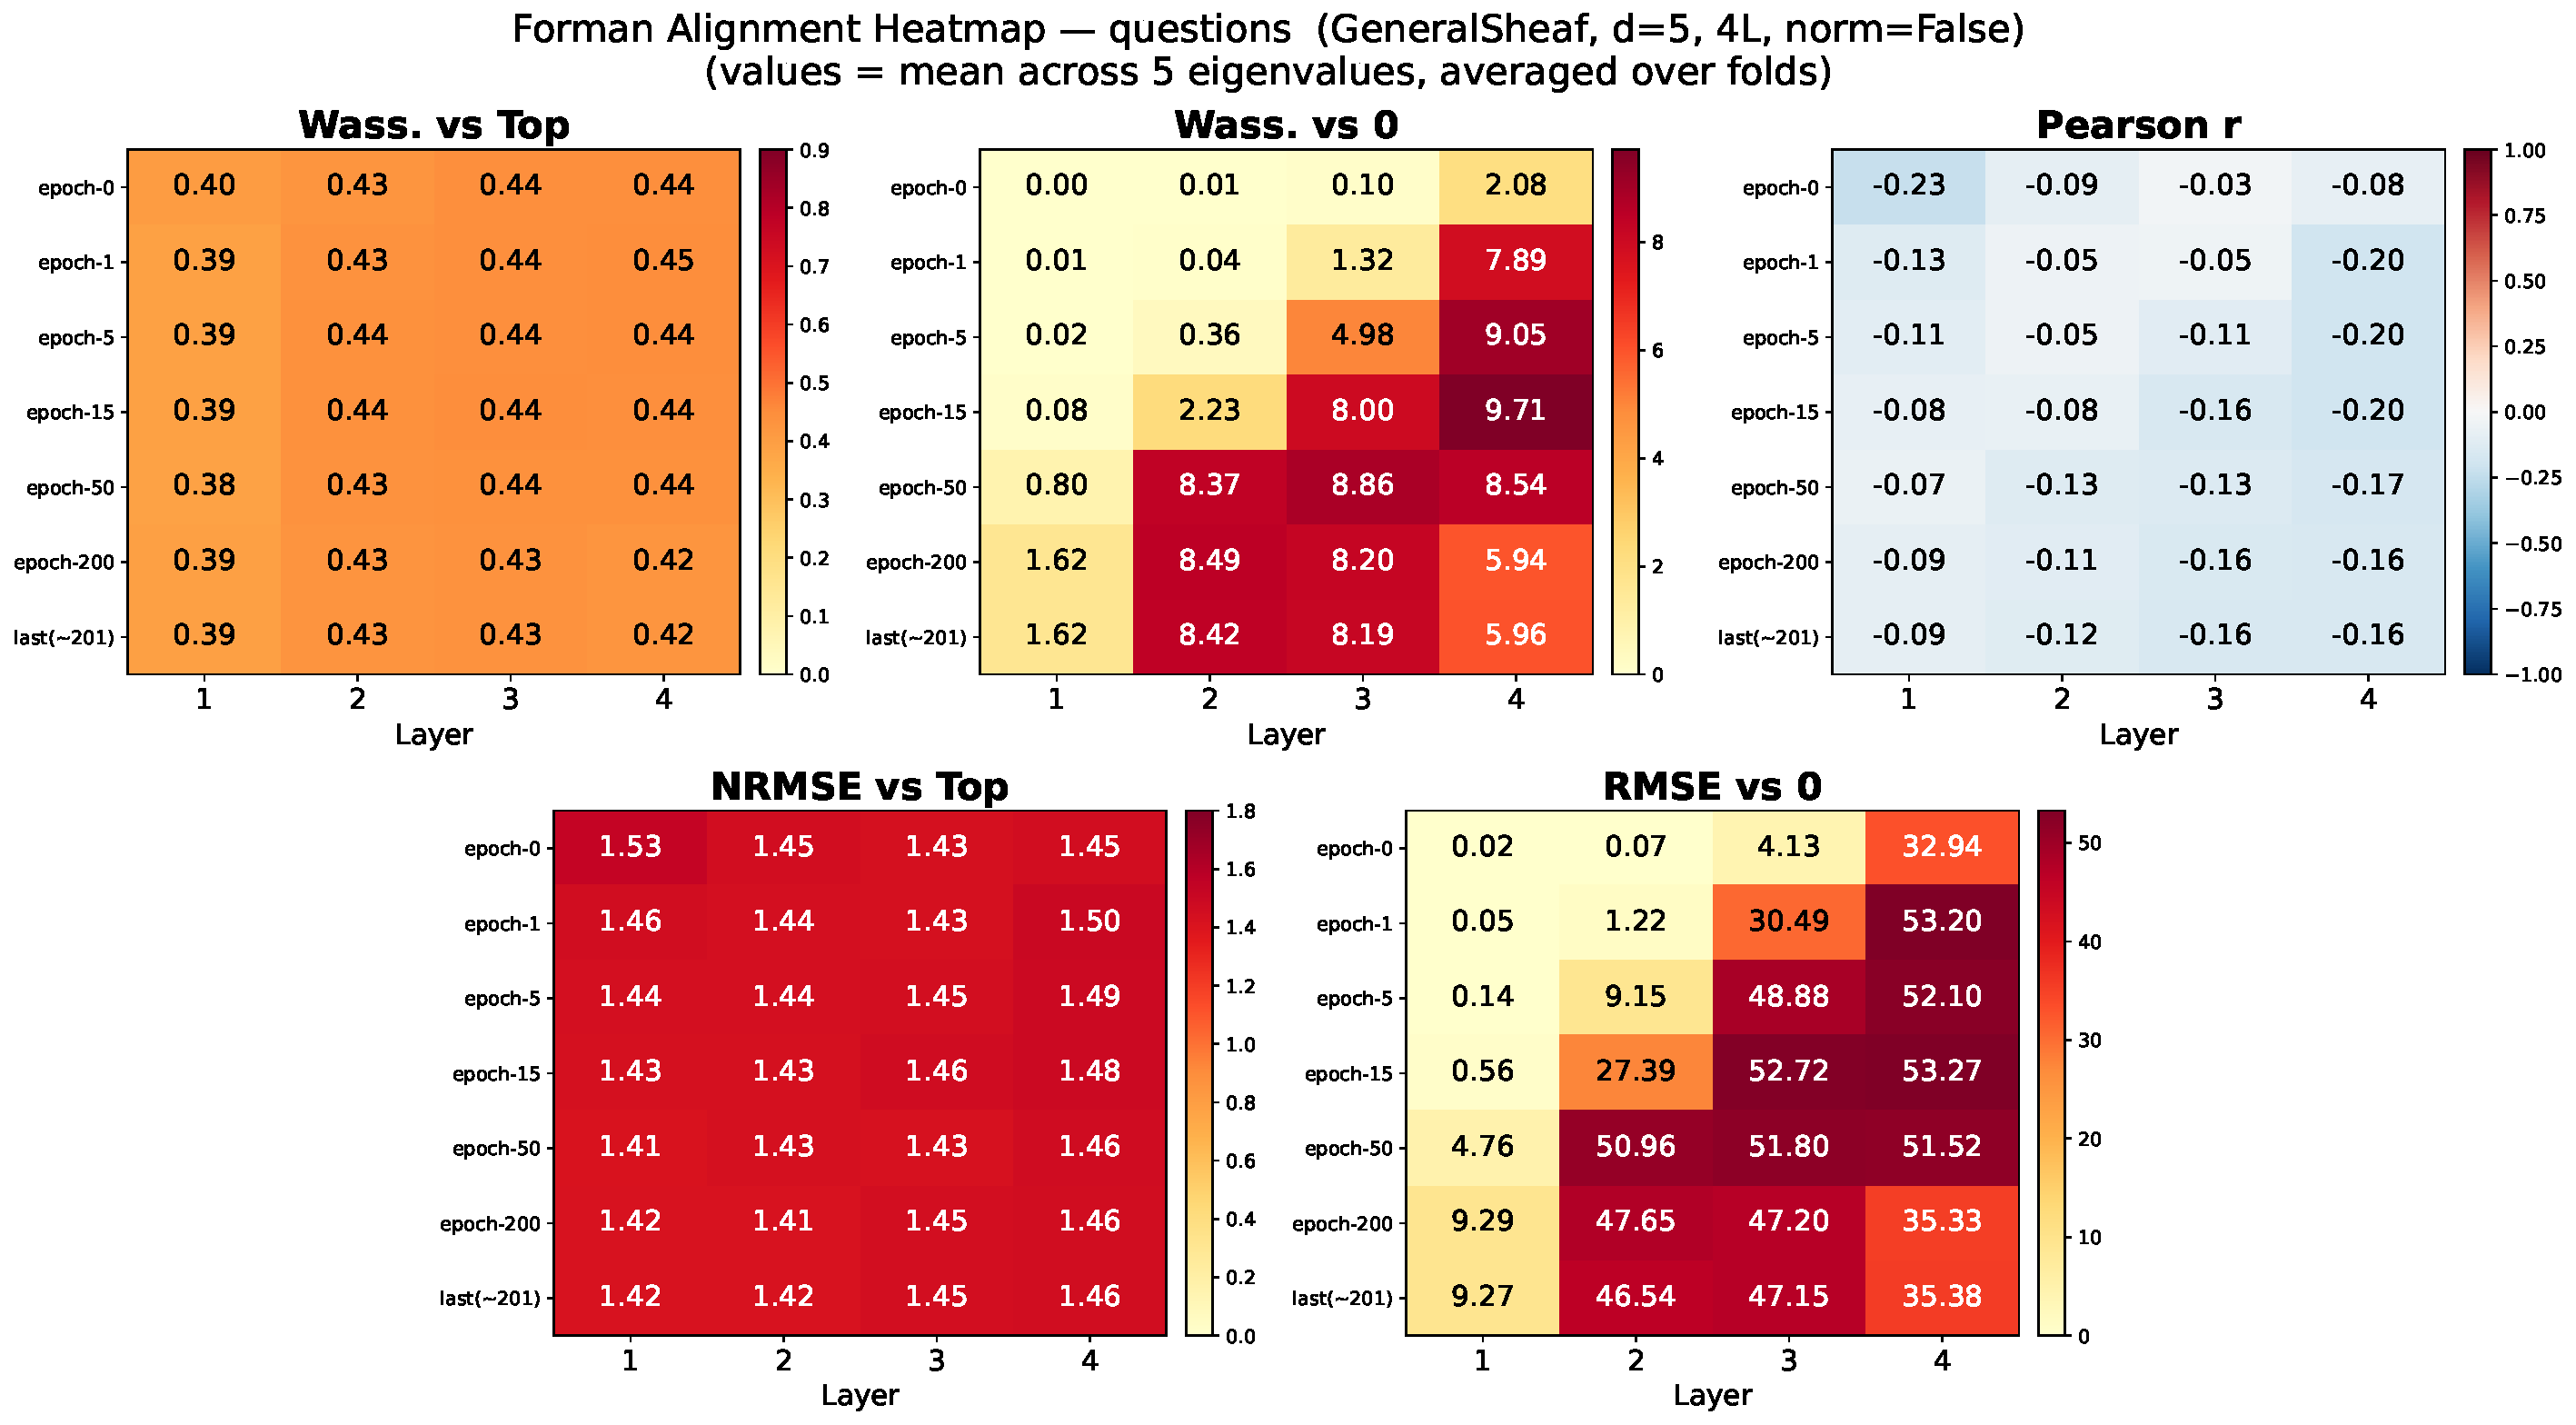
\includegraphics[width=\linewidth]{heatmaps/GeneralSheaf/normalised_false/questions_GeneralSheaf_d5_4L_Norm_False_heatmap.pdf}
\end{figure}
\end{frame}

\begin{frame}{Roman Empire --- GeneralSheaf, $d=5$, $L=5$, Norm=False}
\begin{figure}
    \centering
    
\includegraphics[width=\linewidth]{heatmaps/GeneralSheaf/normalised_false/roman_empire_GeneralSheaf_d5_5L_Norm_False_heatmap.pdf}
\end{figure}
\end{frame}

\begin{frame}{Tolokers --- GeneralSheaf, $d=3$, $L=4$, Norm=False}
\begin{figure}
    \centering
    
\includegraphics[width=\linewidth]{heatmaps/GeneralSheaf/normalised_false/tolokers_GeneralSheaf_d3_4L_Norm_False_heatmap.pdf}
\end{figure}
\end{frame}

\begin{frame}{Wisconsin --- GeneralSheaf, $d=2$, $L=2$, Norm=False}
\begin{figure}
    \centering
    
\includegraphics[width=\linewidth]{heatmaps/GeneralSheaf/normalised_false/wisconsin_GeneralSheaf_d2_2L_Norm_False_heatmap.pdf}
\end{figure}
\end{frame}

% ══════════════════════════════════════════════════════════════════════════════
%  SECTION 3 — Cross-comparison Direction A: both normalised, different training objectives
% ══════════════════════════════════════════════════════════════════════════════

\begin{frame}{}
\centering
\Huge\textbf{Cross-Comparison --- Direction A}\\[6pt]
\Large Both profiles: normalised $\widetilde{\Delta}_{\mathcal{F}}$\\[4pt]
\large Maps from \texttt{norm=True} training \textbf{vs} maps from \texttt{norm=False} training\\[4pt]
\normalsize (same Laplacian normalisation, different training objective)
\end{frame}

\begin{frame}{Amazon Ratings --- Dir A: maps norm=True vs maps norm=False (both normalised $\widetilde{\Delta}_{\mathcal{F}}$)}
\begin{figure}
    \centering
    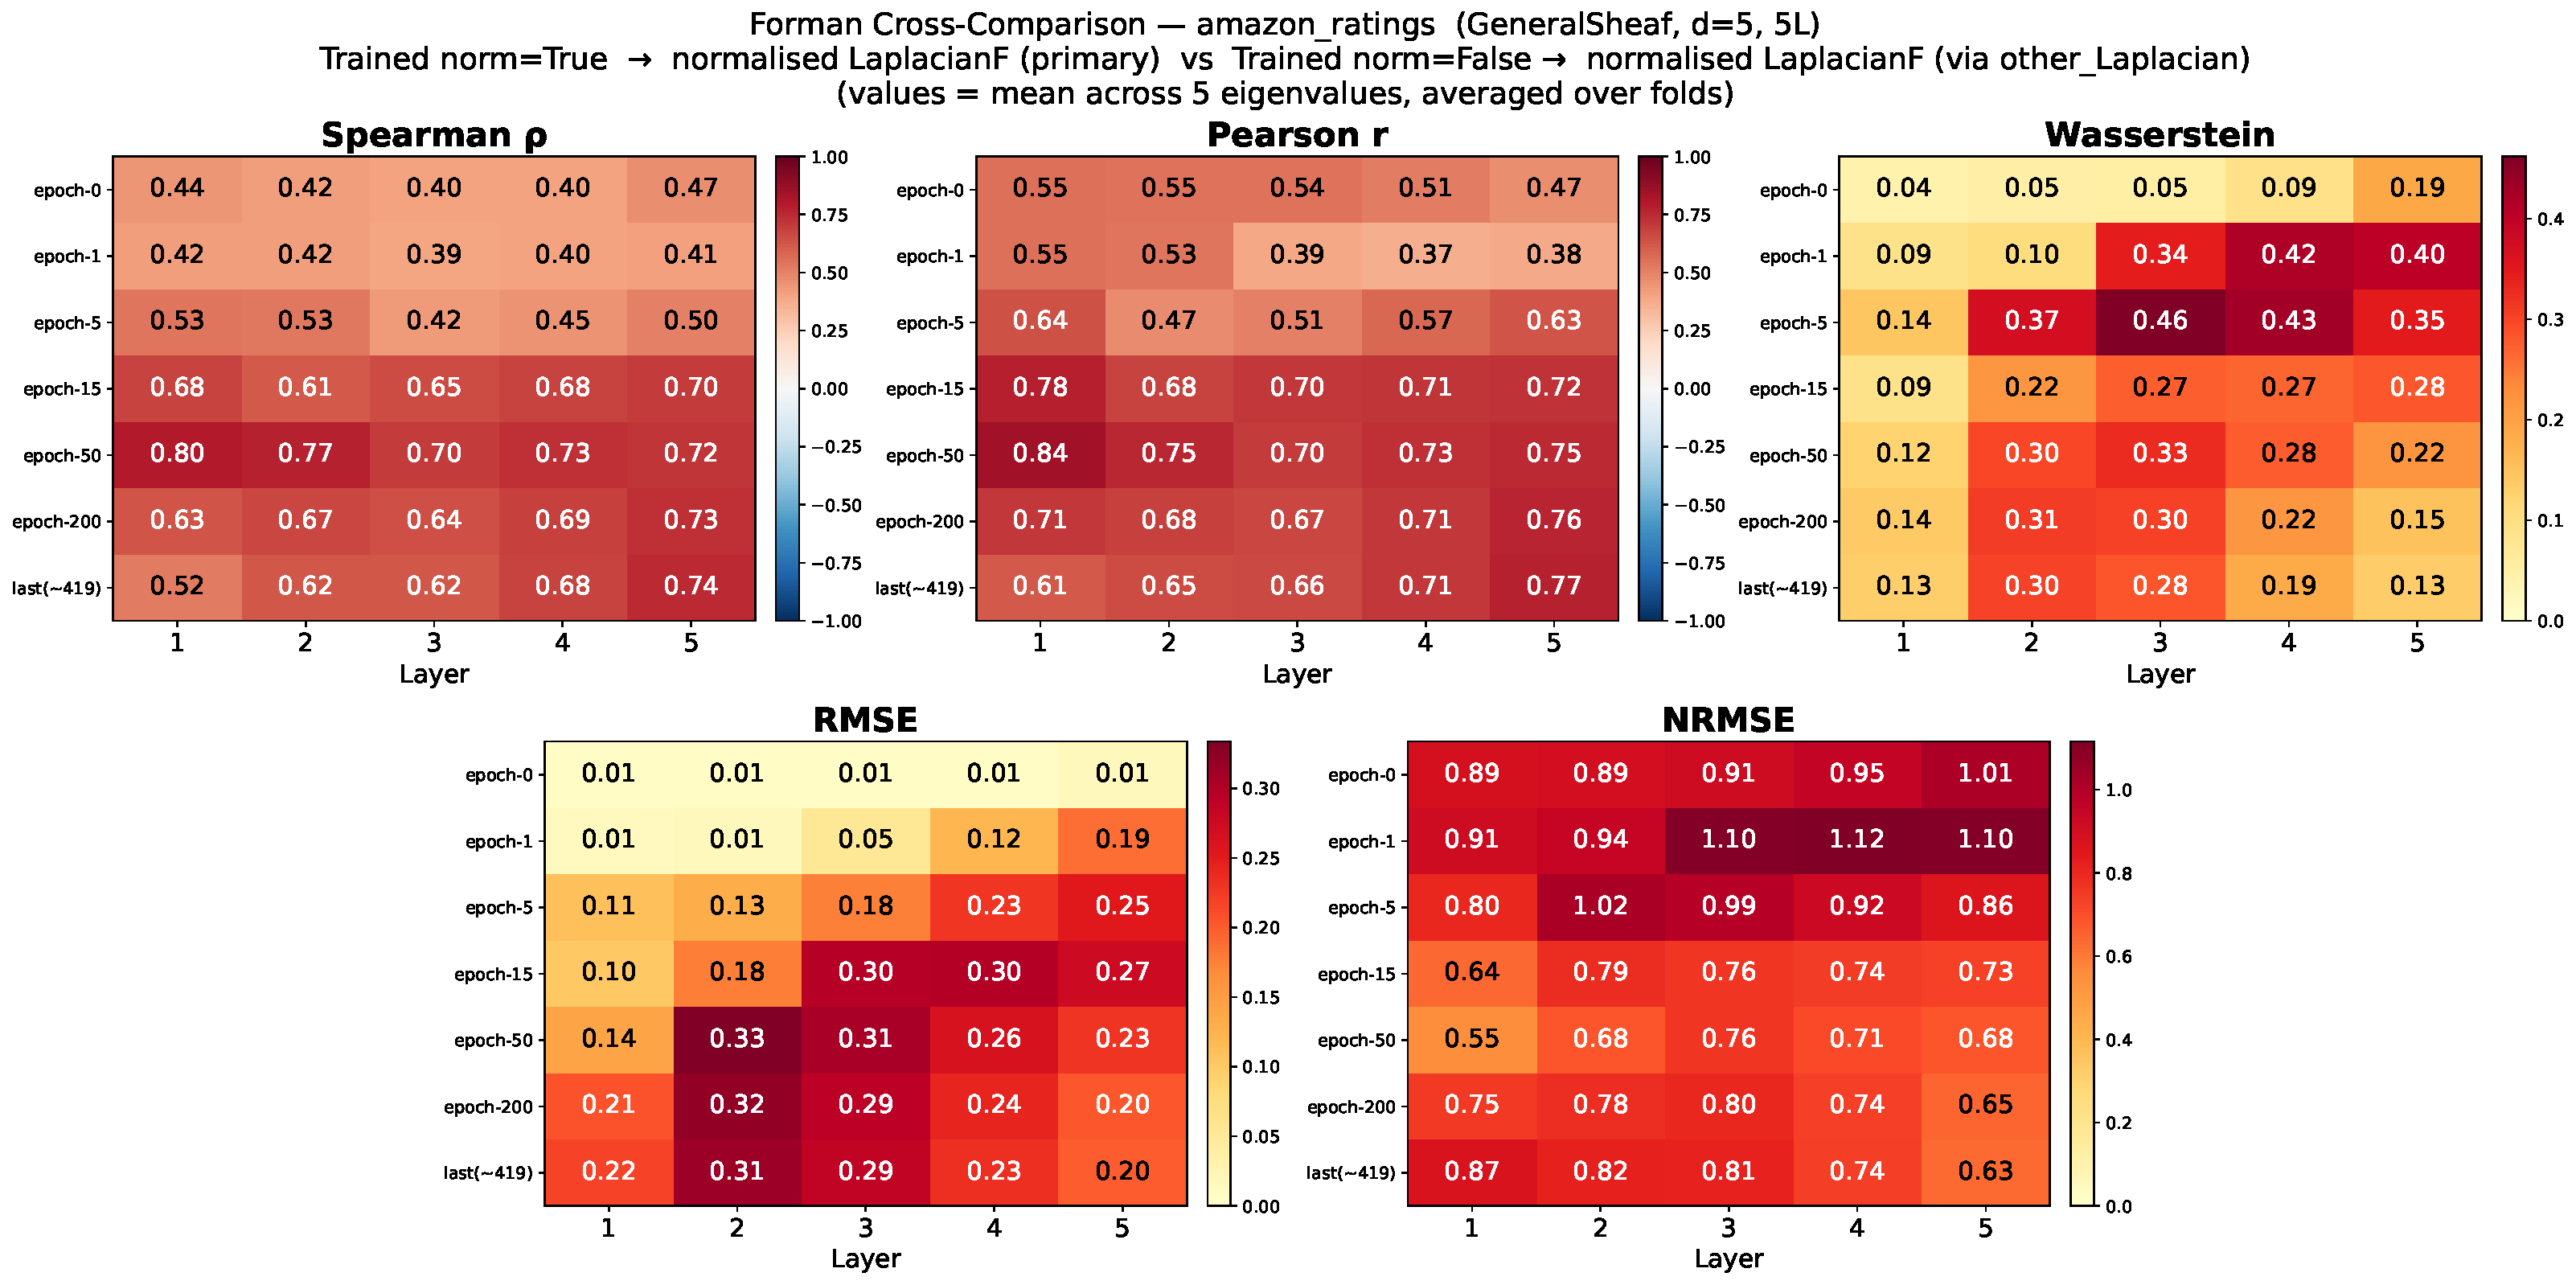
\includegraphics[width=\linewidth]{heatmaps/comparison/norm_true_vs_other_norm_false/amazon_ratings_GeneralSheaf_d5_5L_norm_true_primary_vs_other_norm_false_heatmap.pdf}
\end{figure}
\end{frame}

\begin{frame}{Citeseer --- Dir A: maps norm=True vs maps norm=False (both normalised $\widetilde{\Delta}_{\mathcal{F}}$)}
\begin{figure}
    \centering
    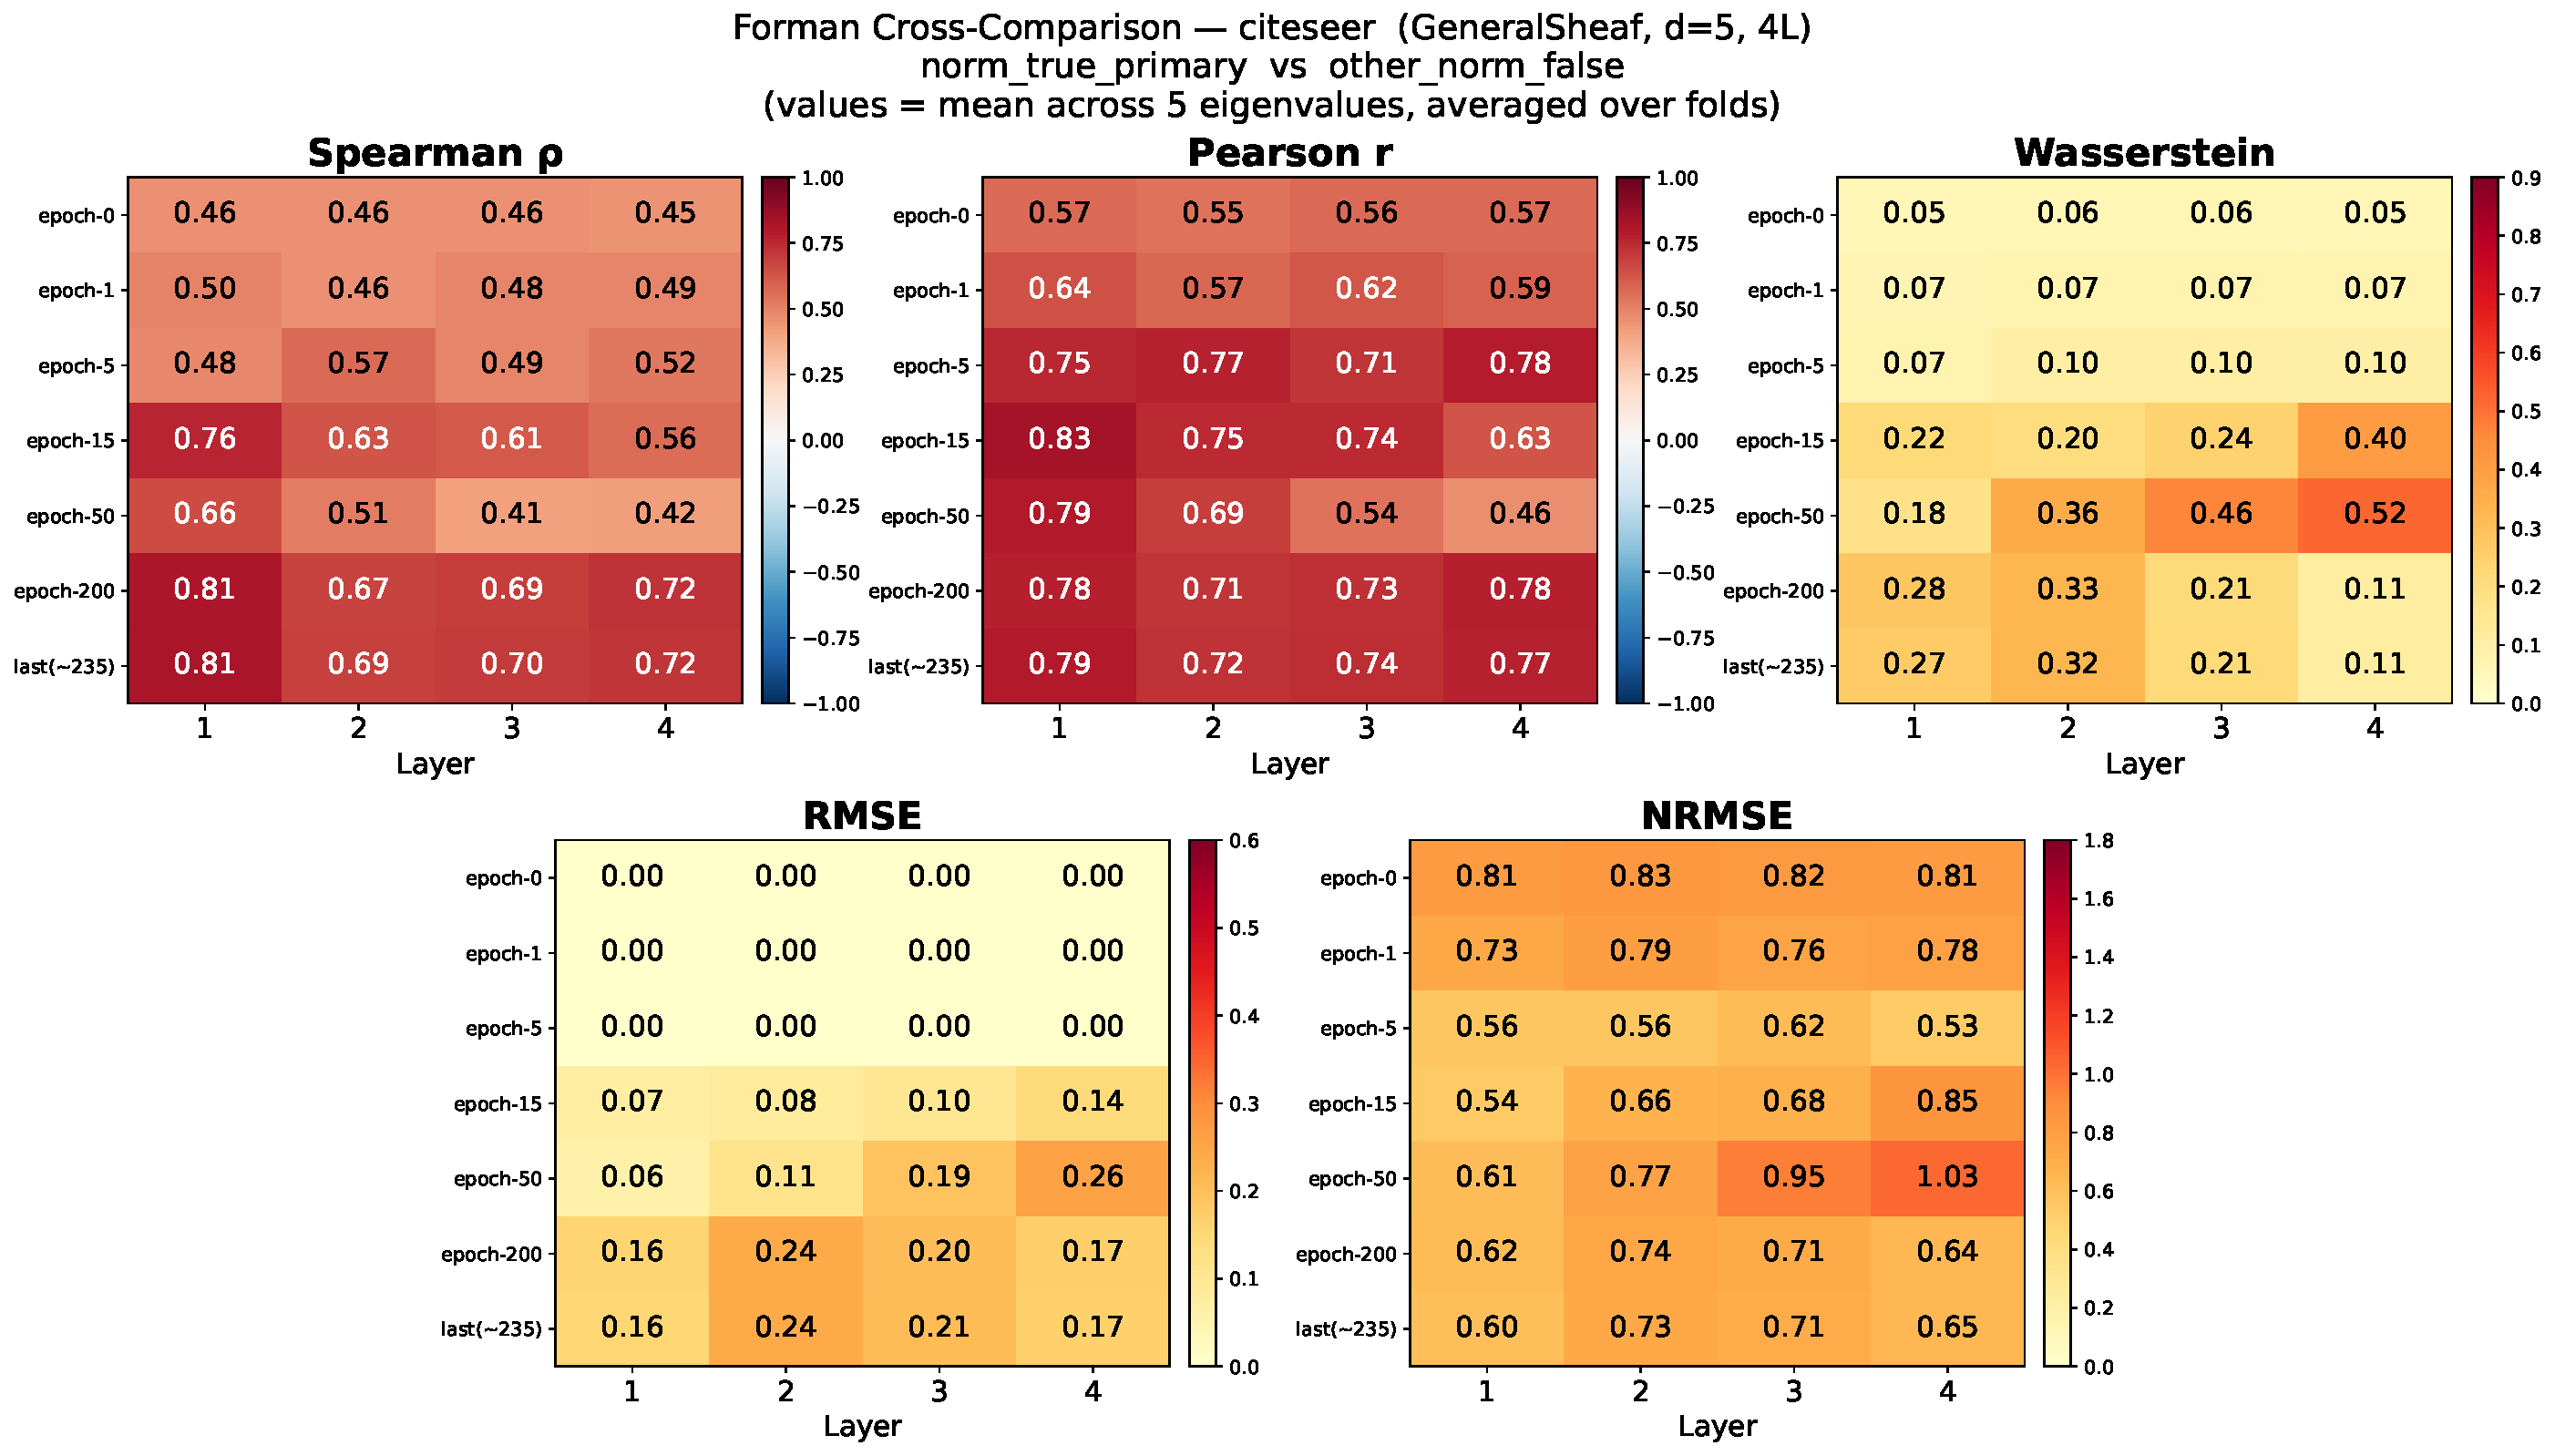
\includegraphics[width=\linewidth]{heatmaps/comparison/norm_true_vs_other_norm_false/citeseer_GeneralSheaf_d5_4L_norm_true_primary_vs_other_norm_false_heatmap.pdf}
\end{figure}
\end{frame}

\begin{frame}{Cora --- Dir A: maps norm=True vs maps norm=False (both normalised $\widetilde{\Delta}_{\mathcal{F}}$)}
\begin{figure}
    \centering
    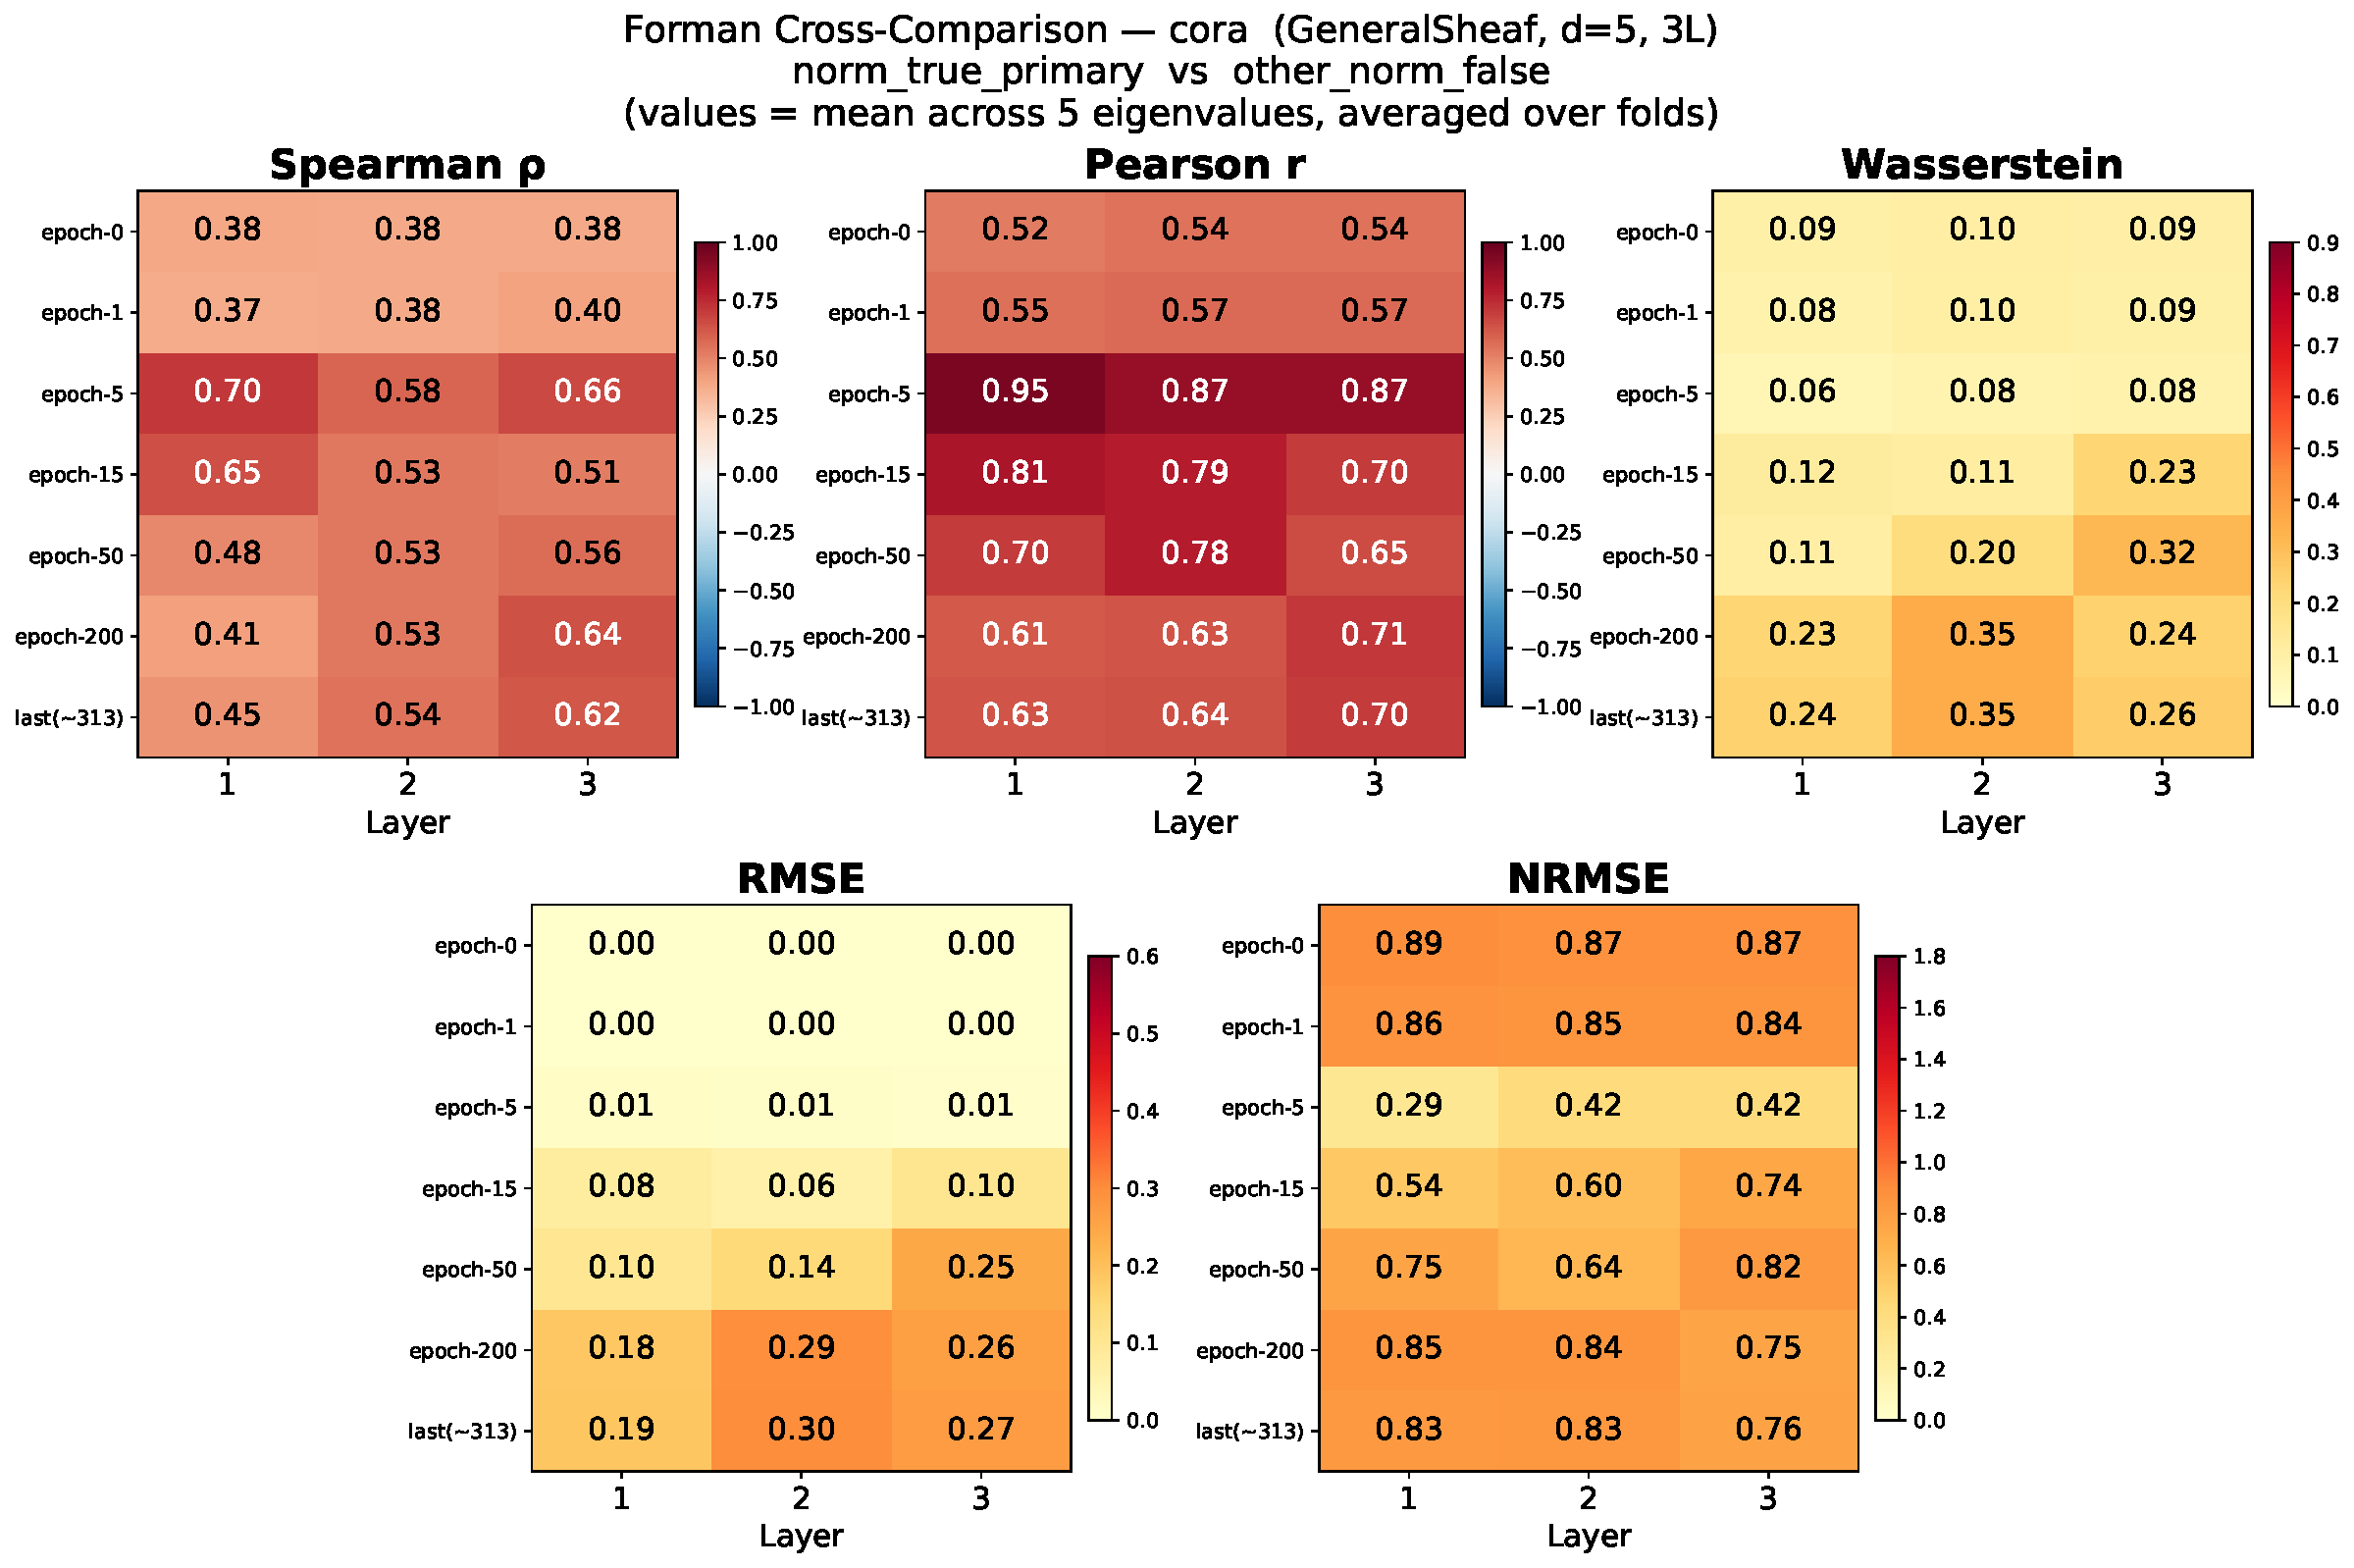
\includegraphics[width=\linewidth]{heatmaps/comparison/norm_true_vs_other_norm_false/cora_GeneralSheaf_d5_3L_norm_true_primary_vs_other_norm_false_heatmap.pdf}
\end{figure}
\end{frame}

\begin{frame}{Cornell --- Dir A: maps norm=True vs maps norm=False (both normalised $\widetilde{\Delta}_{\mathcal{F}}$)}
\begin{figure}
    \centering
    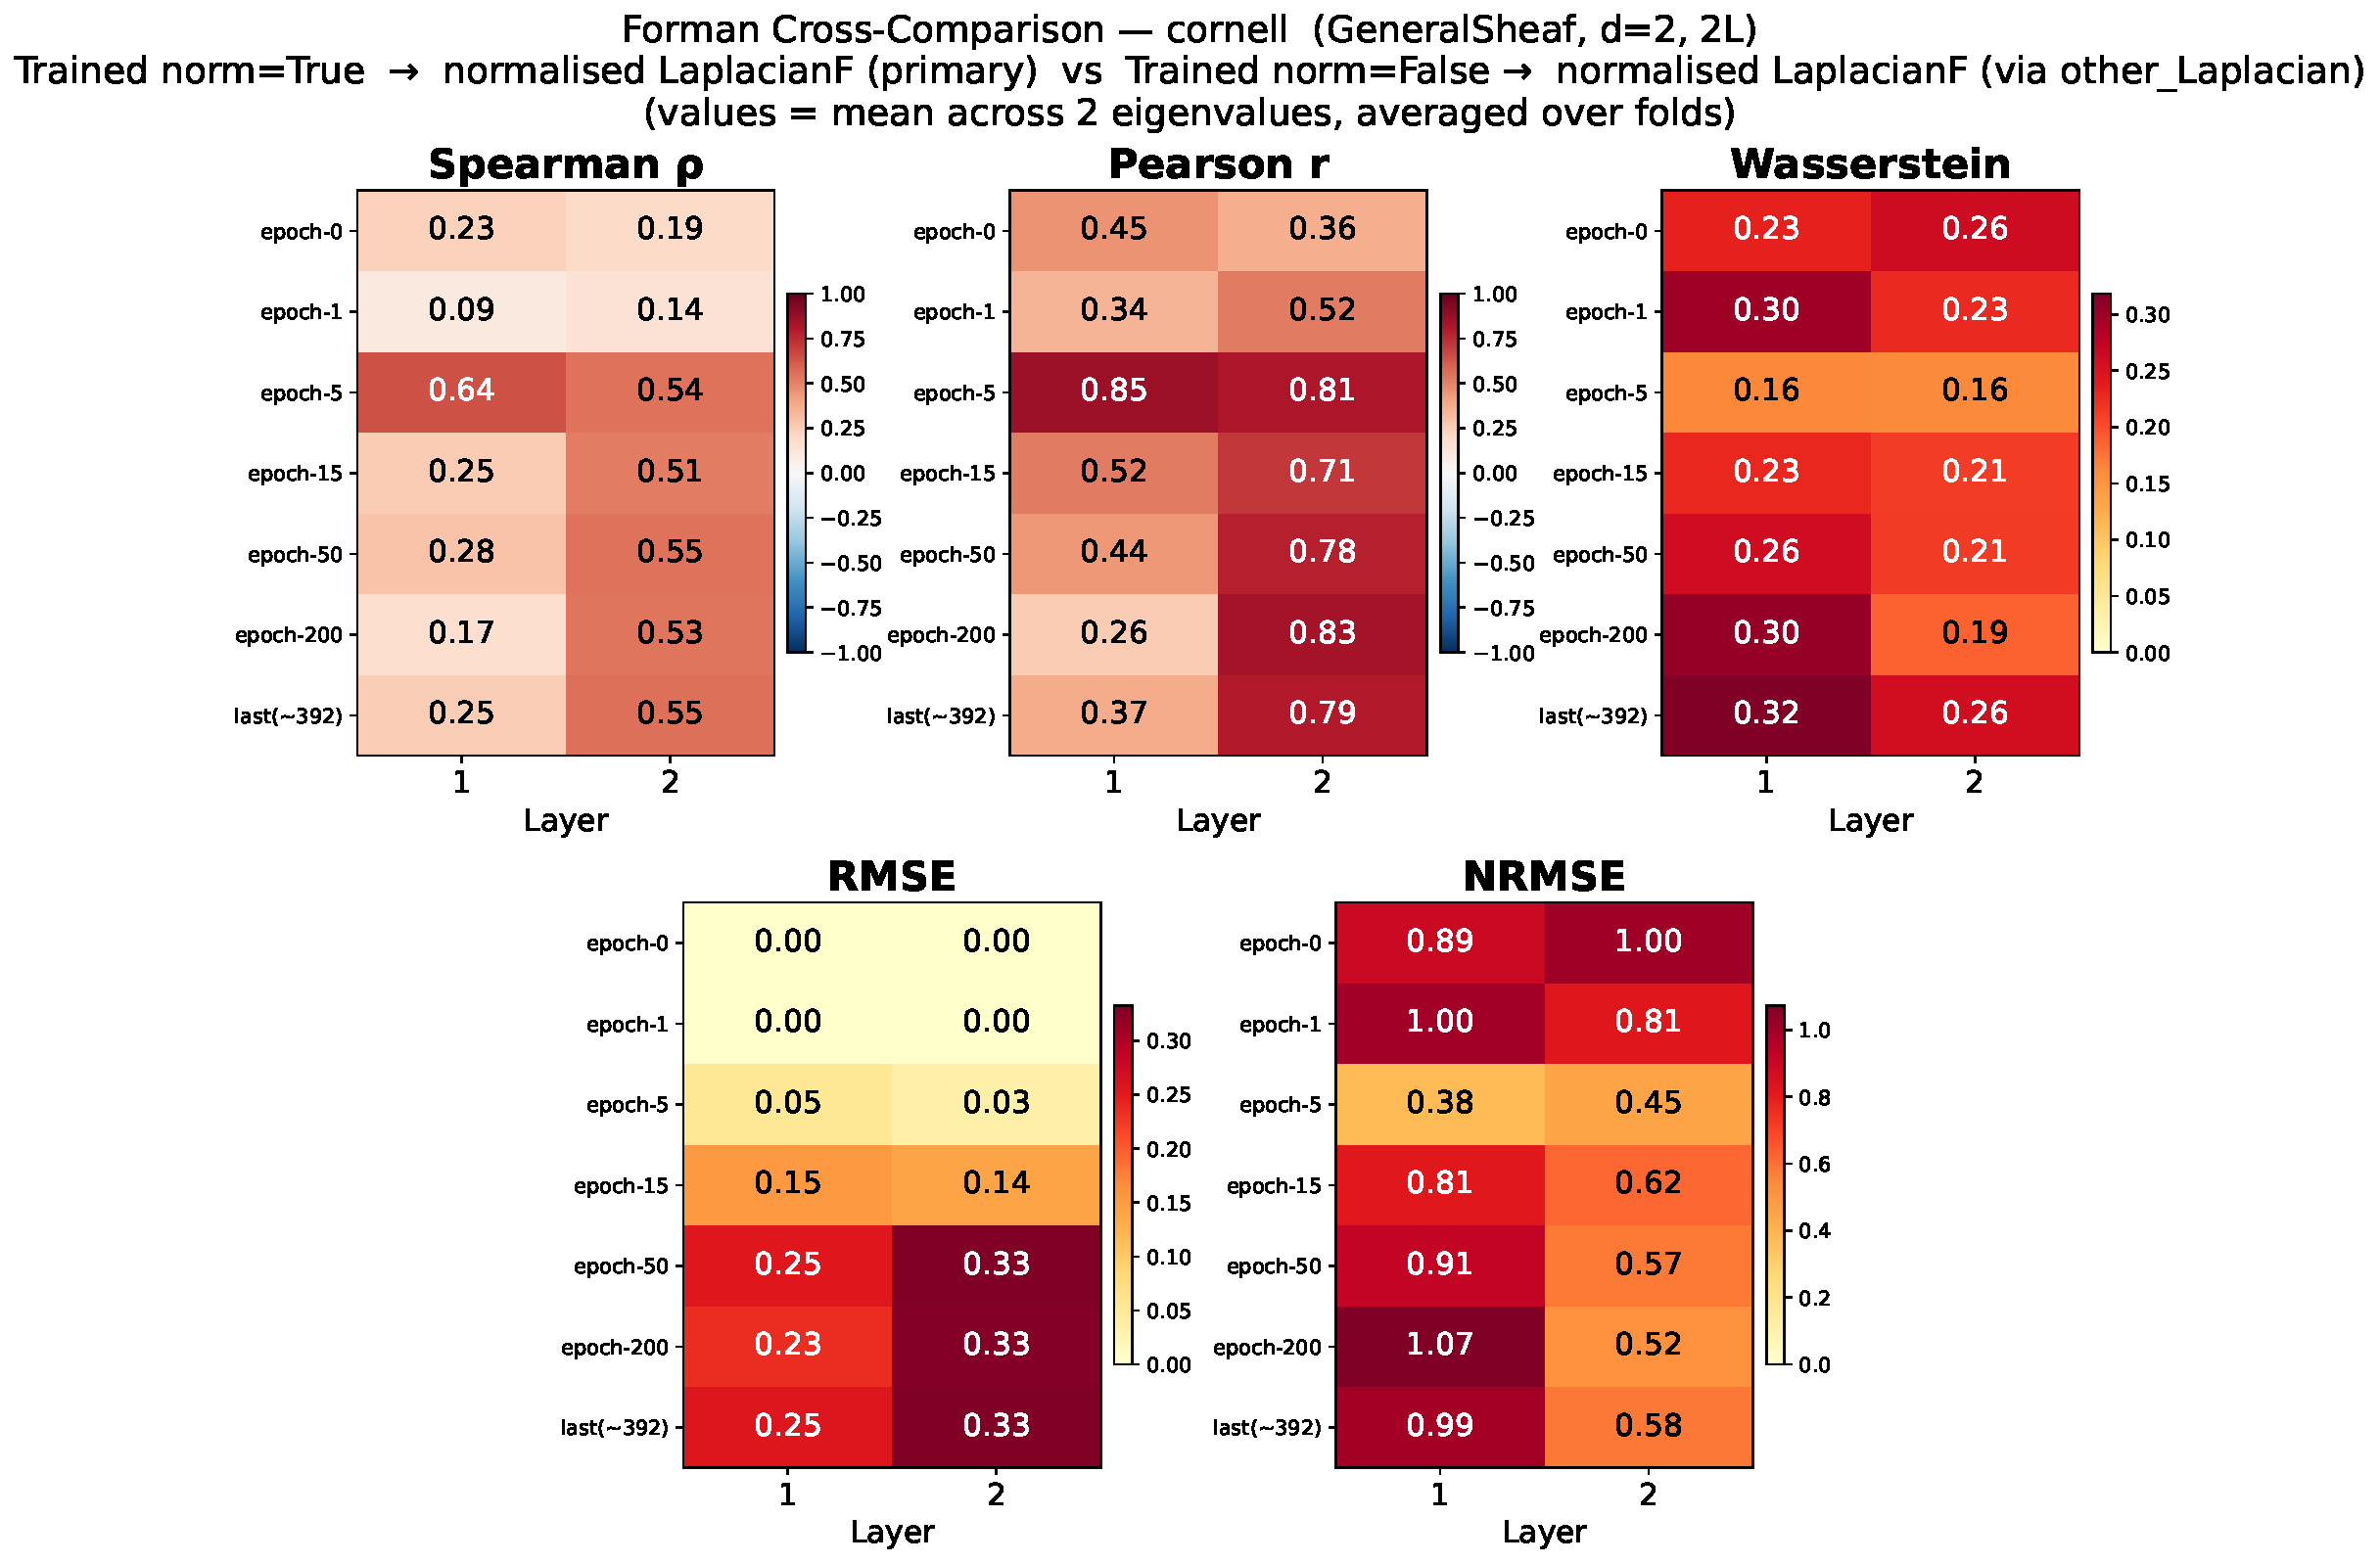
\includegraphics[width=\linewidth]{heatmaps/comparison/norm_true_vs_other_norm_false/cornell_GeneralSheaf_d2_2L_norm_true_primary_vs_other_norm_false_heatmap.pdf}
\end{figure}
\end{frame}

\begin{frame}{Minesweeper --- Dir A: maps norm=True vs maps norm=False (both normalised $\widetilde{\Delta}_{\mathcal{F}}$)}
\begin{figure}
    \centering
    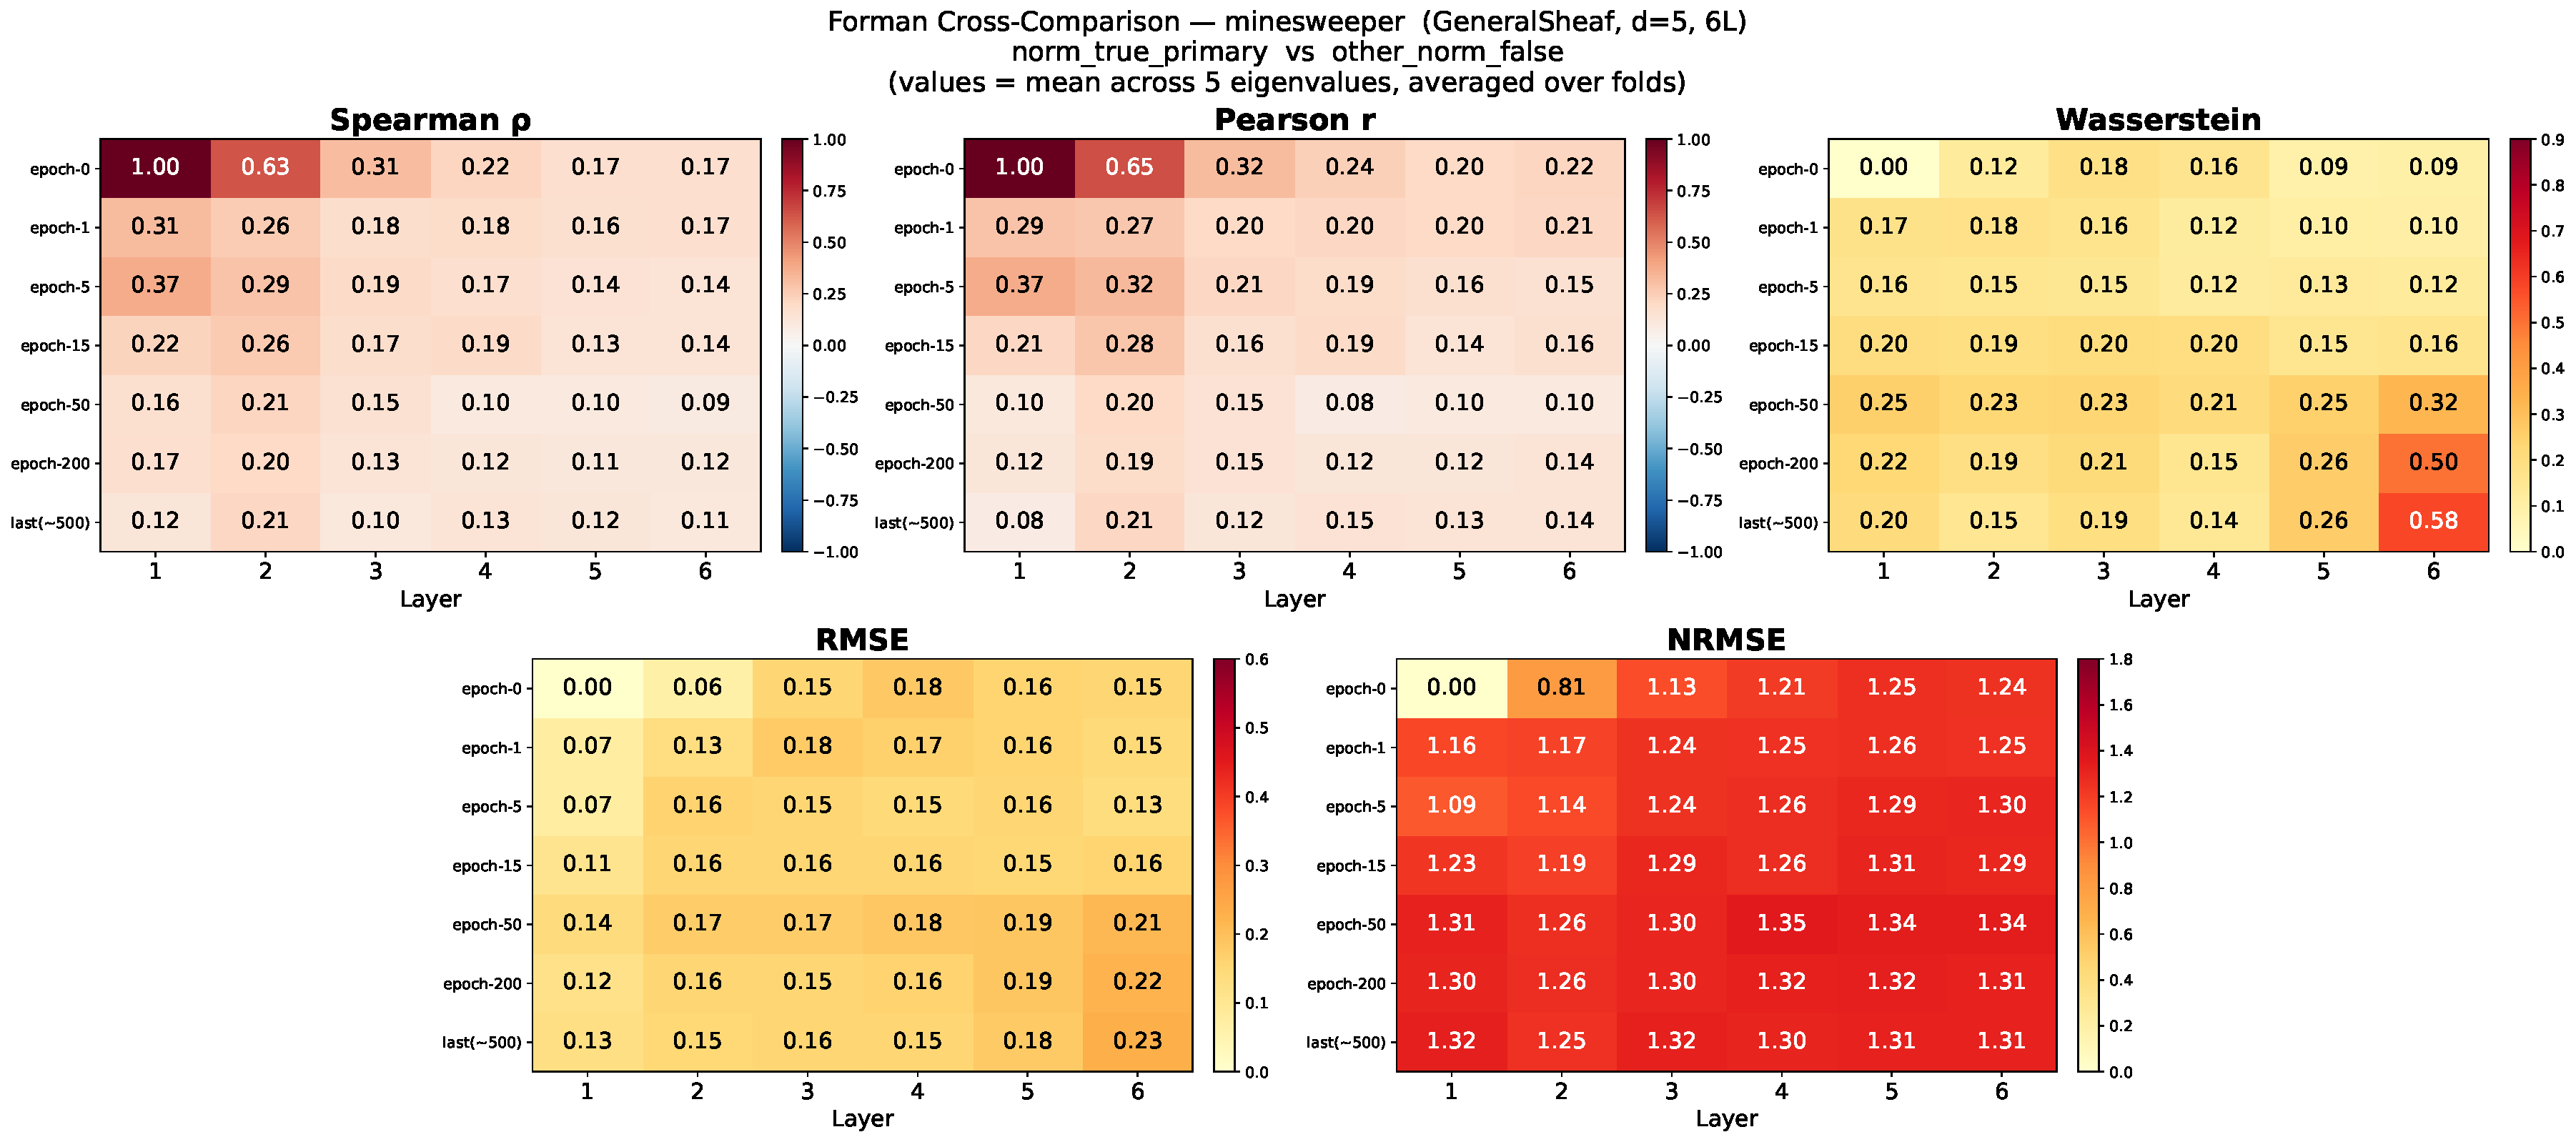
\includegraphics[width=\linewidth]{heatmaps/comparison/norm_true_vs_other_norm_false/minesweeper_GeneralSheaf_d5_6L_norm_true_primary_vs_other_norm_false_heatmap.pdf}
\end{figure}
\end{frame}

\begin{frame}{Pubmed --- Dir A: maps norm=True vs maps norm=False (both normalised $\widetilde{\Delta}_{\mathcal{F}}$)}
\begin{figure}
    \centering
    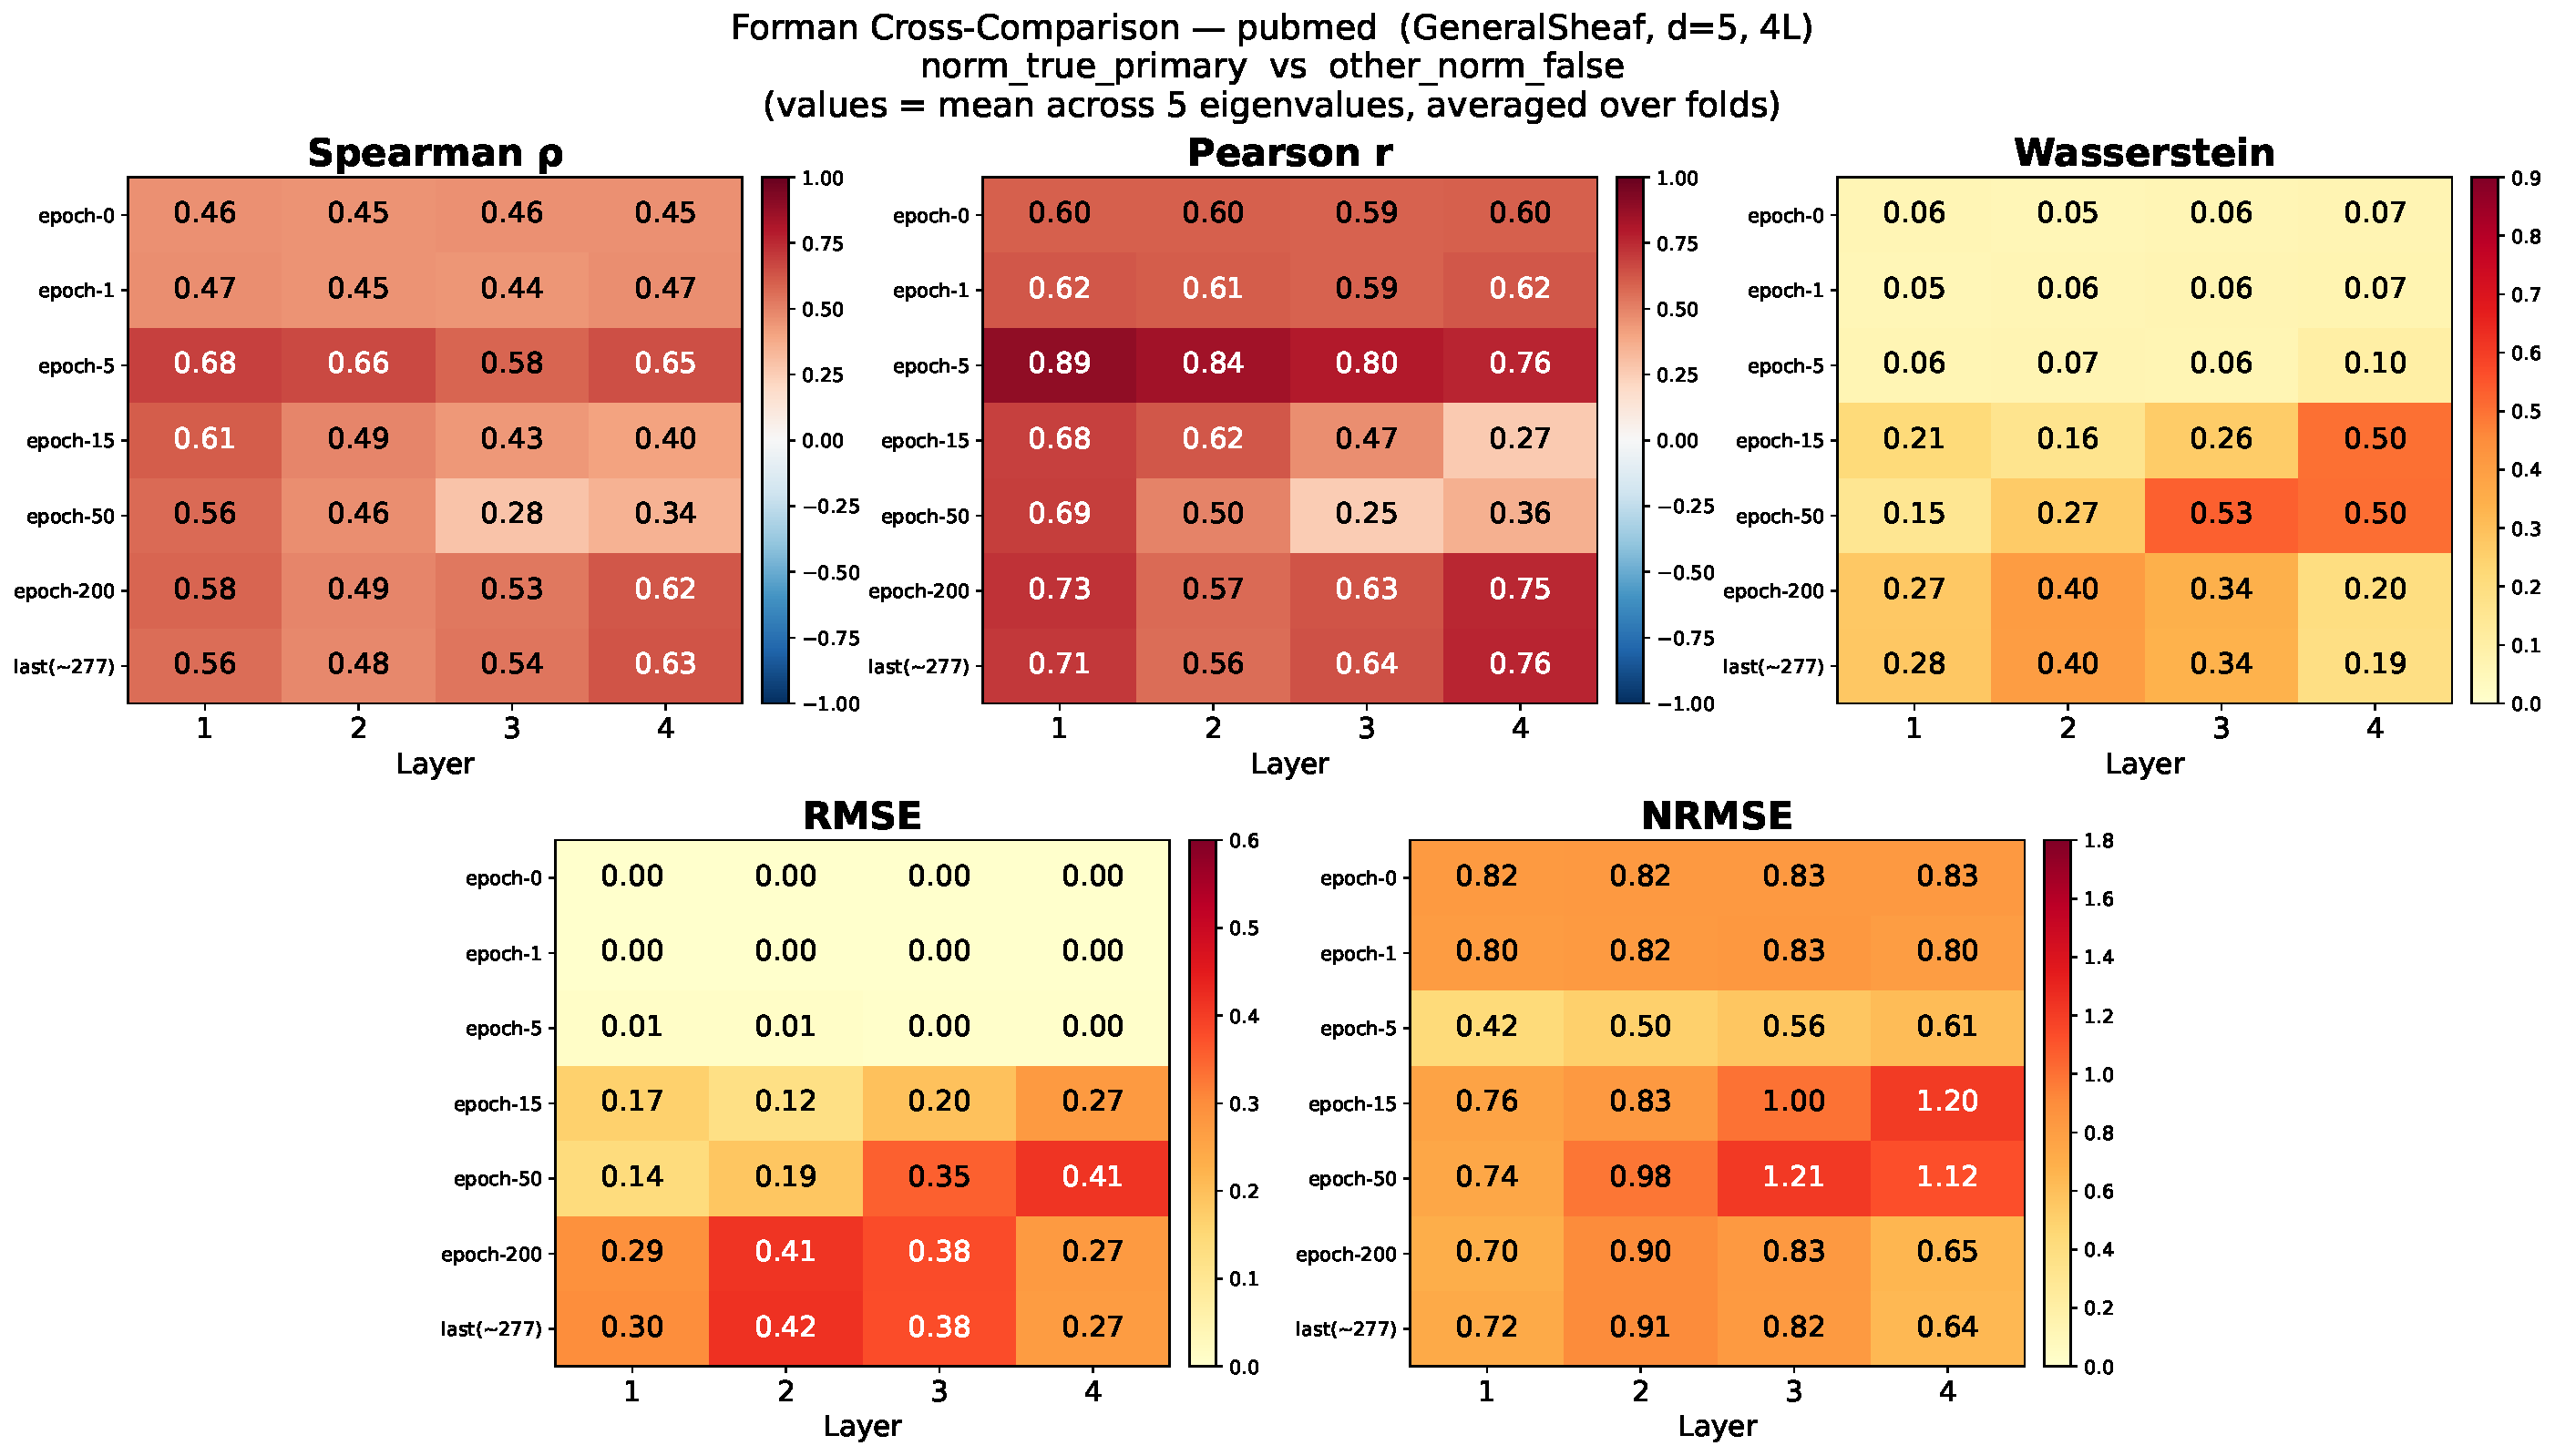
\includegraphics[width=\linewidth]{heatmaps/comparison/norm_true_vs_other_norm_false/pubmed_GeneralSheaf_d5_4L_norm_true_primary_vs_other_norm_false_heatmap.pdf}
\end{figure}
\end{frame}

\begin{frame}{Questions --- Dir A: maps norm=True vs maps norm=False (both normalised $\widetilde{\Delta}_{\mathcal{F}}$)}
\begin{figure}
    \centering
    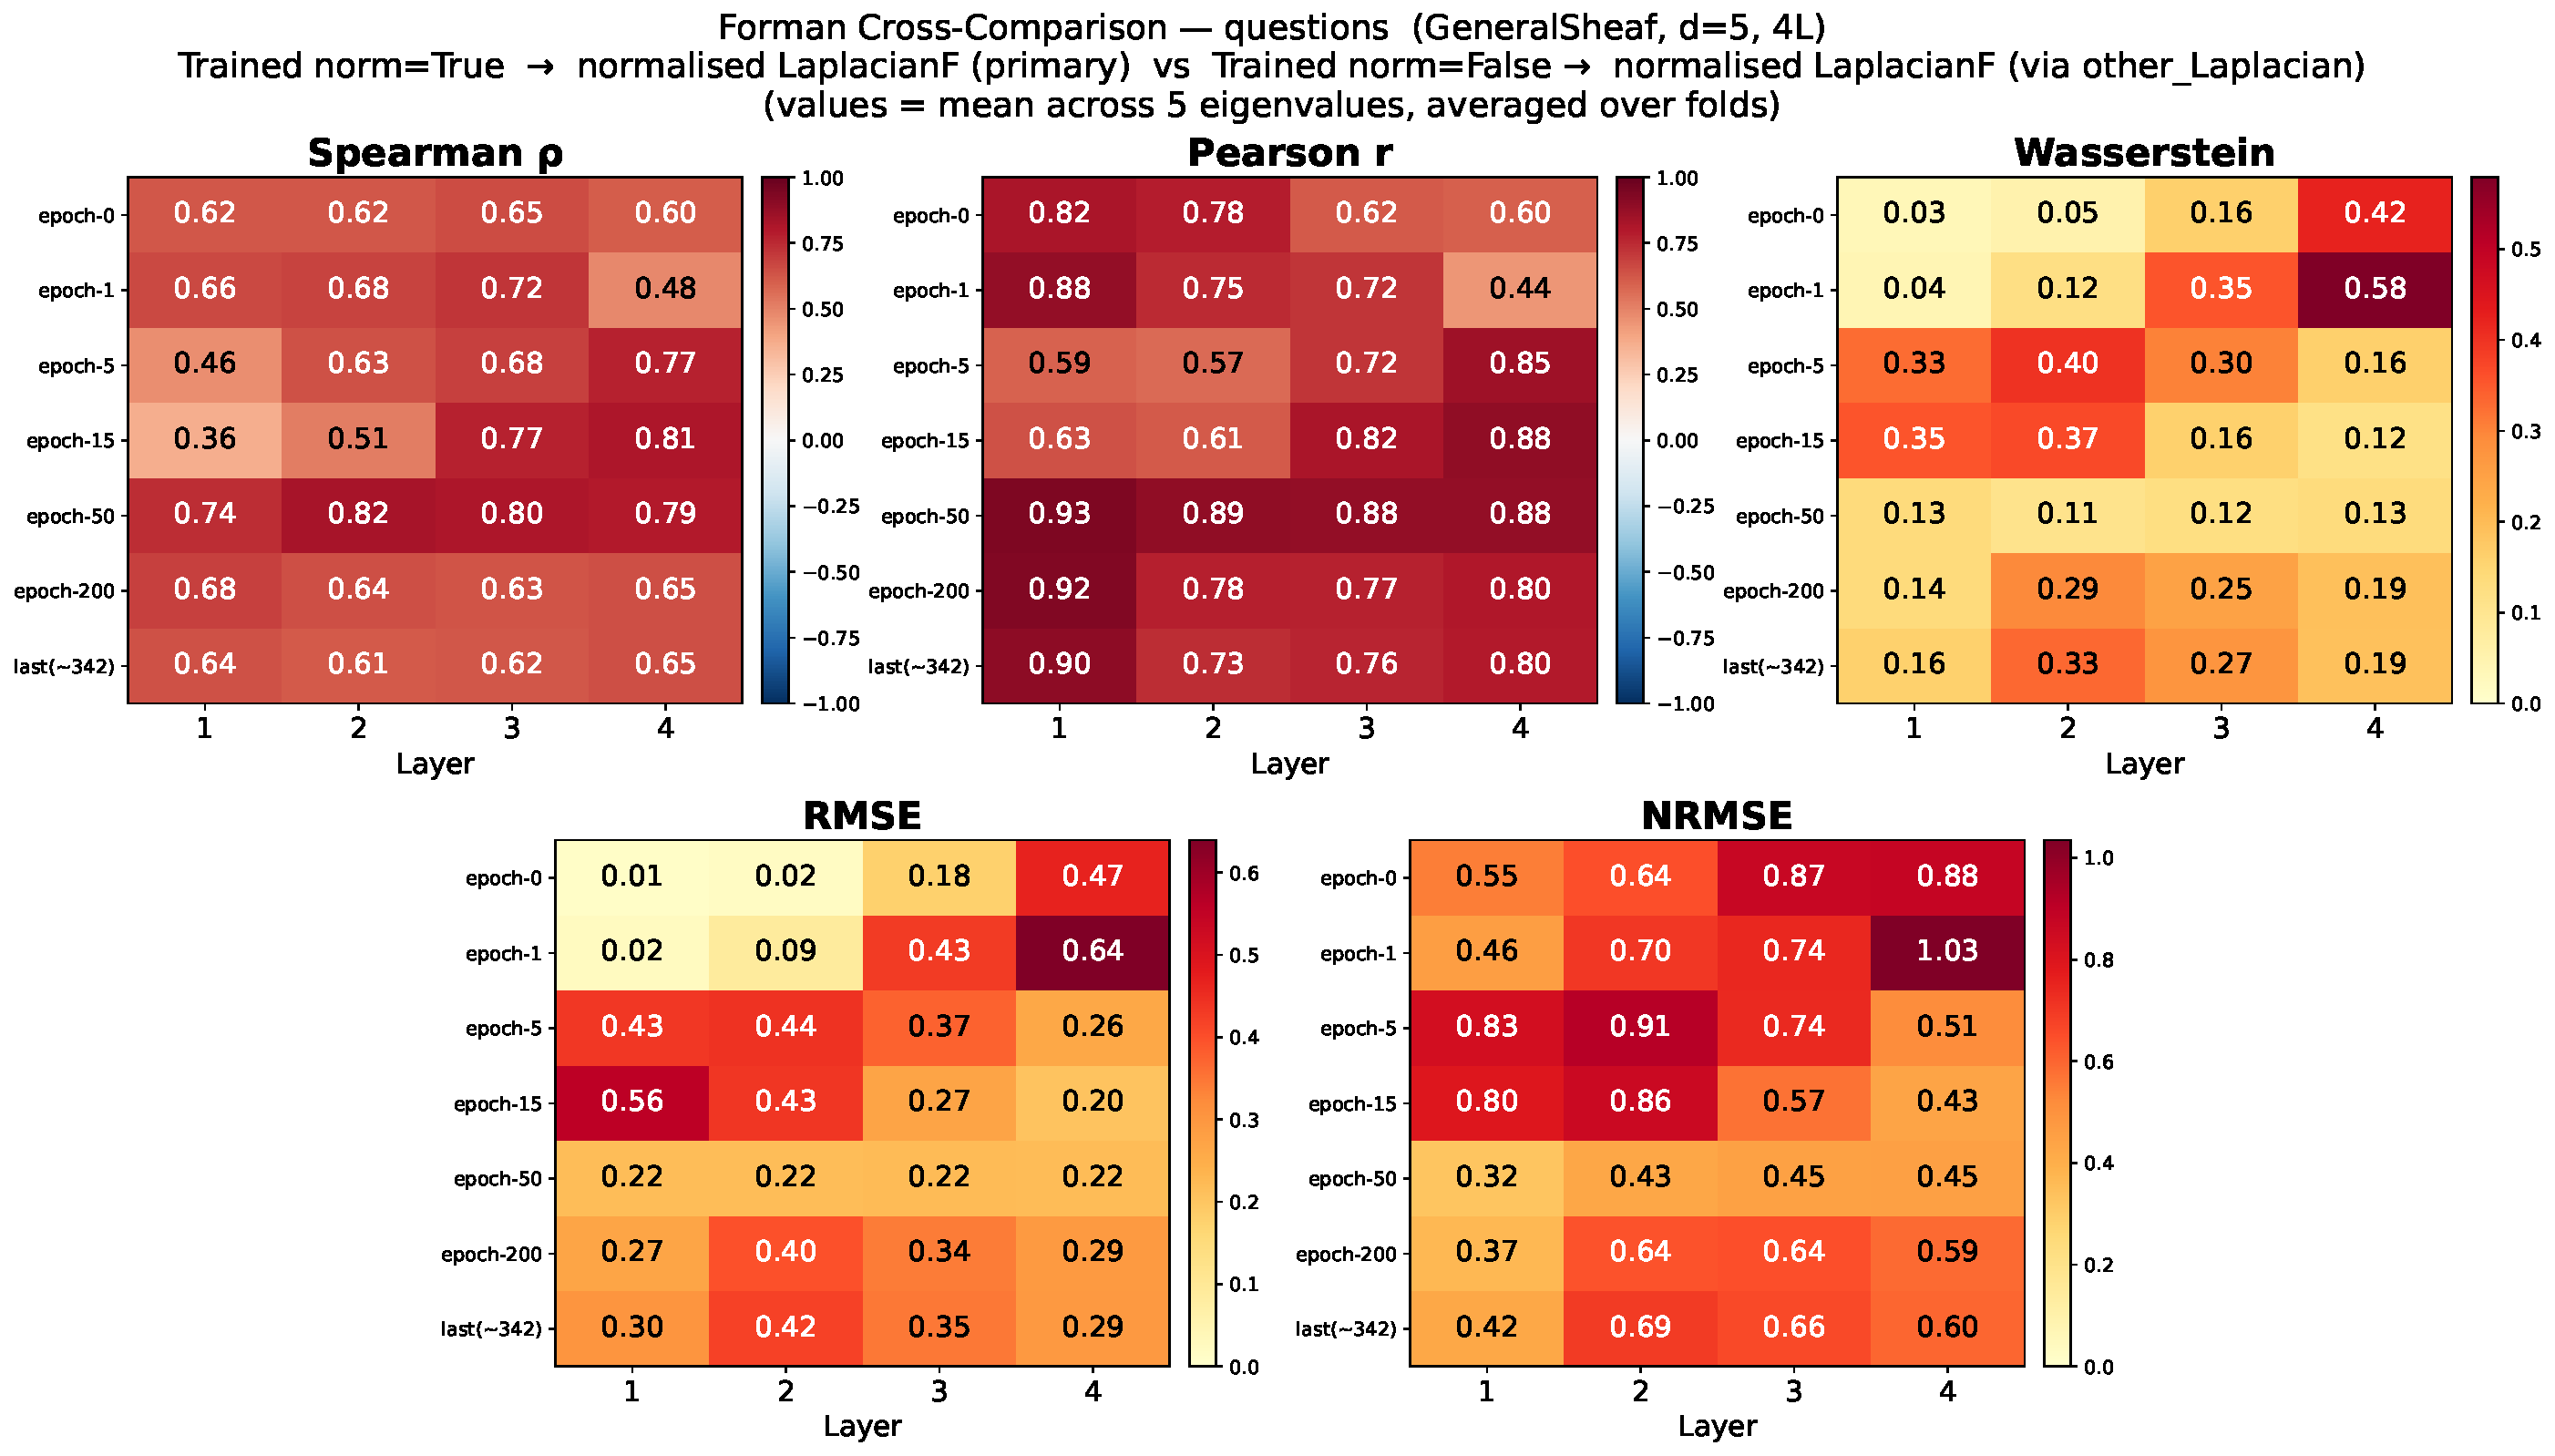
\includegraphics[width=\linewidth]{heatmaps/comparison/norm_true_vs_other_norm_false/questions_GeneralSheaf_d5_4L_norm_true_primary_vs_other_norm_false_heatmap.pdf}
\end{figure}
\end{frame}

\begin{frame}{Roman Empire --- Dir A: maps norm=True vs maps norm=False (both normalised $\widetilde{\Delta}_{\mathcal{F}}$)}
\begin{figure}
    \centering
    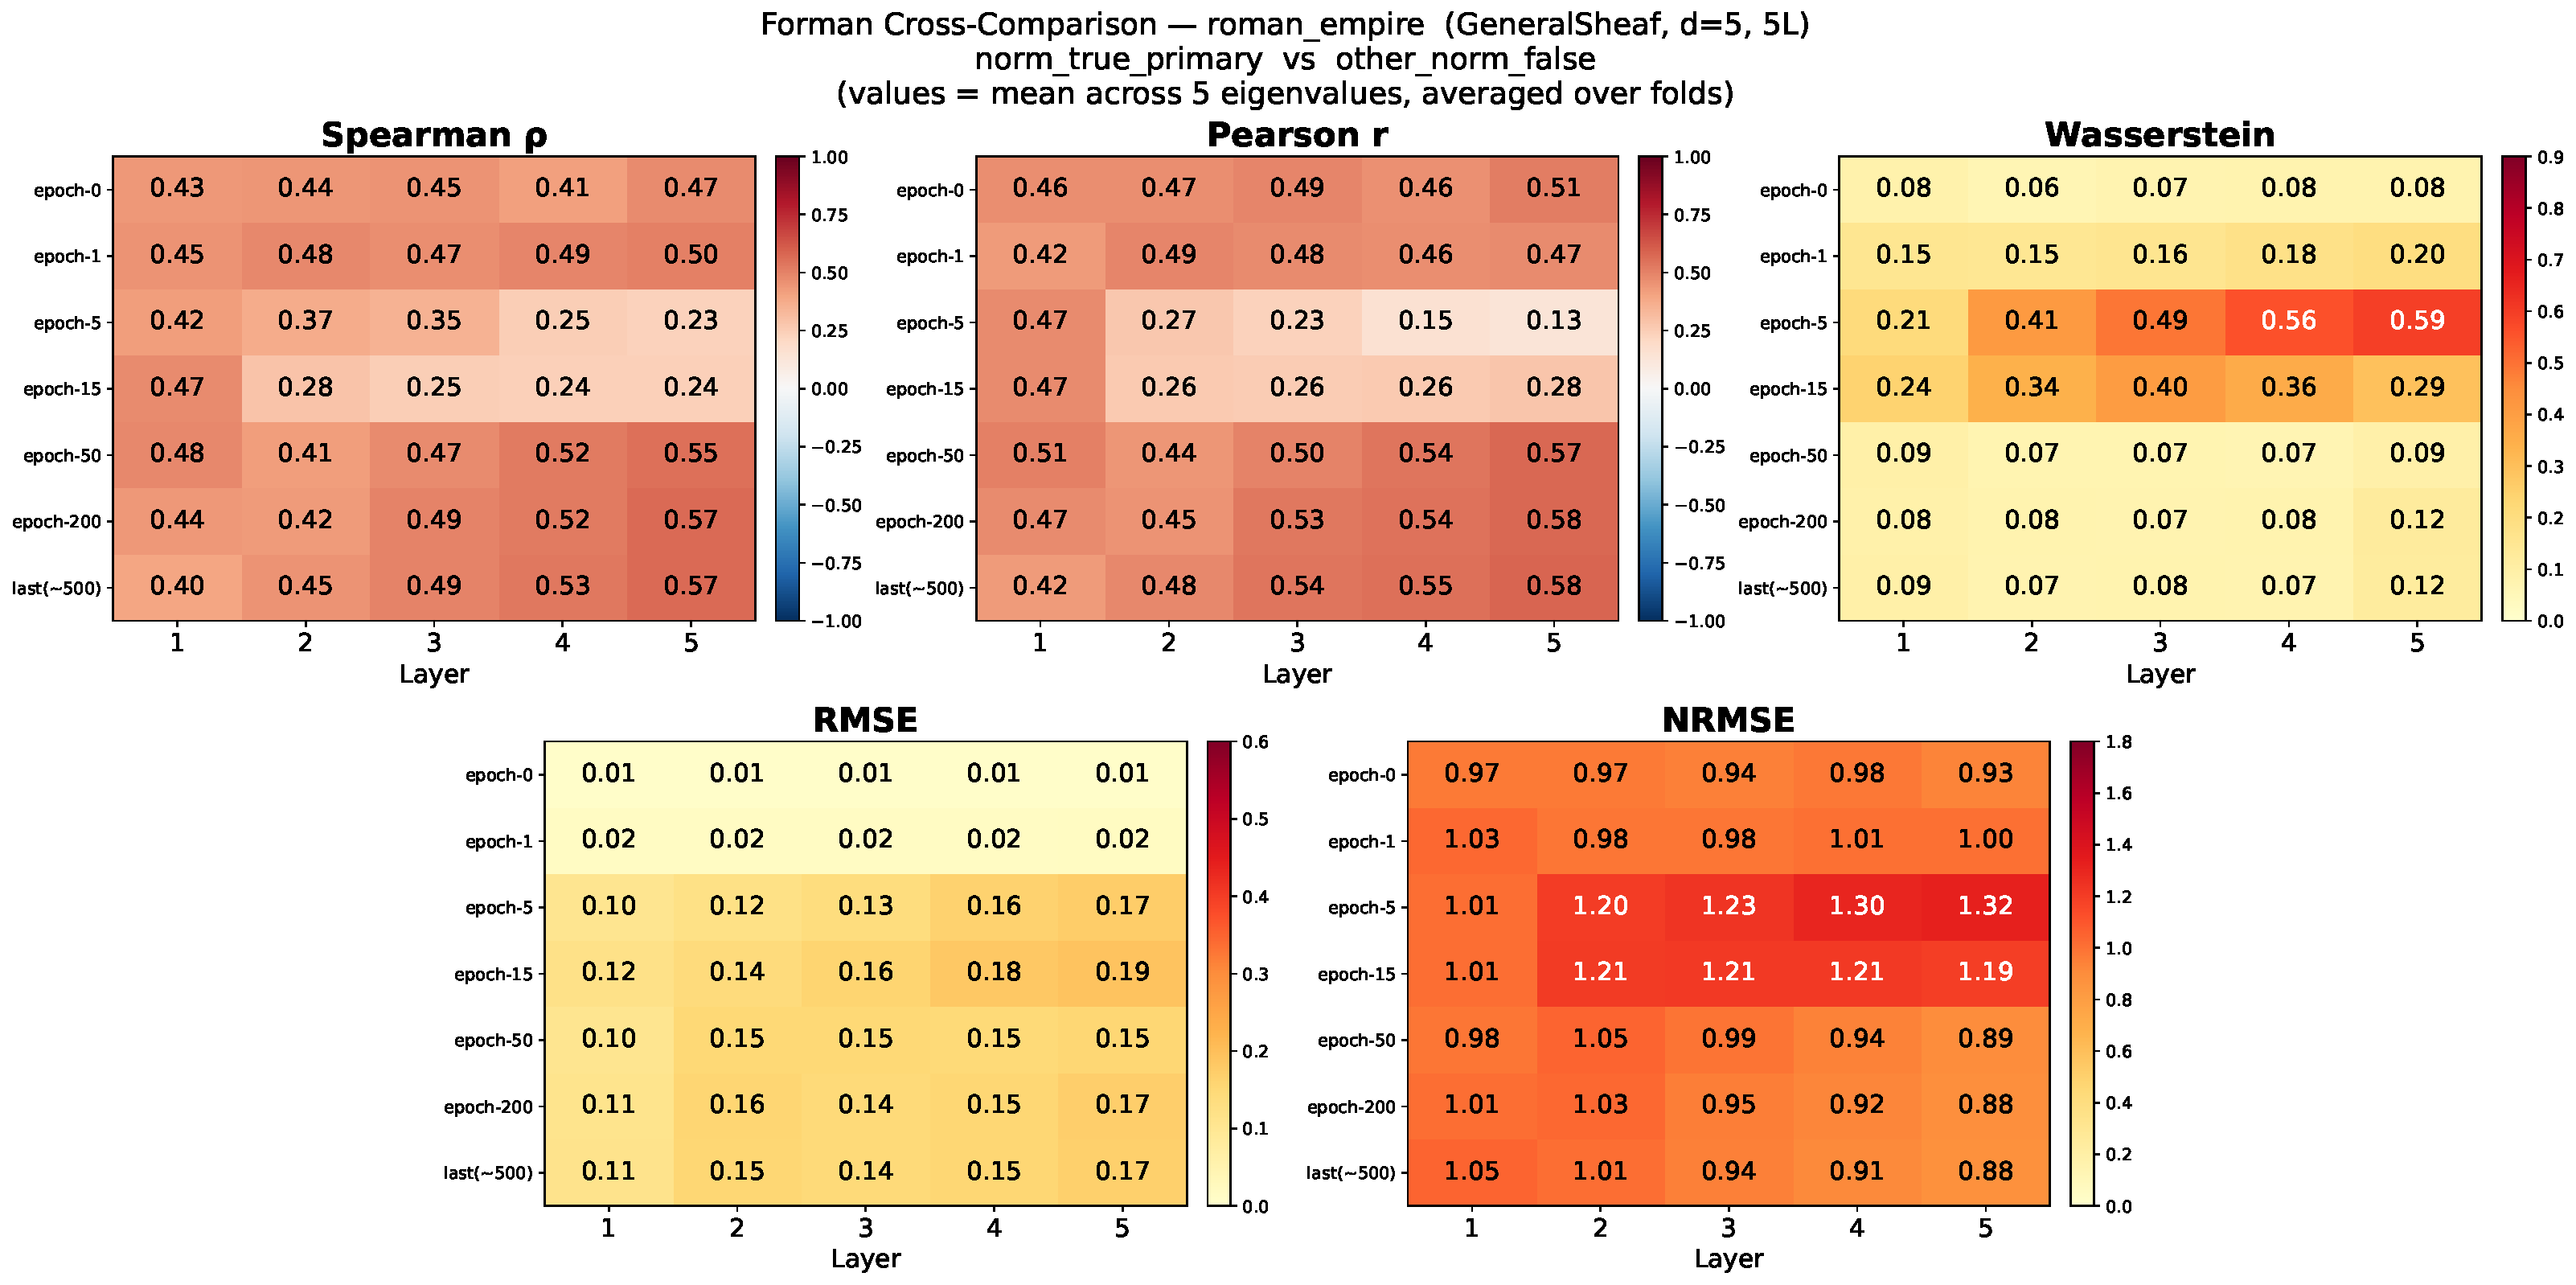
\includegraphics[width=\linewidth]{heatmaps/comparison/norm_true_vs_other_norm_false/roman_empire_GeneralSheaf_d5_5L_norm_true_primary_vs_other_norm_false_heatmap.pdf}
\end{figure}
\end{frame}

\begin{frame}{Tolokers --- Dir A: maps norm=True vs maps norm=False (both normalised $\widetilde{\Delta}_{\mathcal{F}}$)}
\begin{figure}
    \centering
    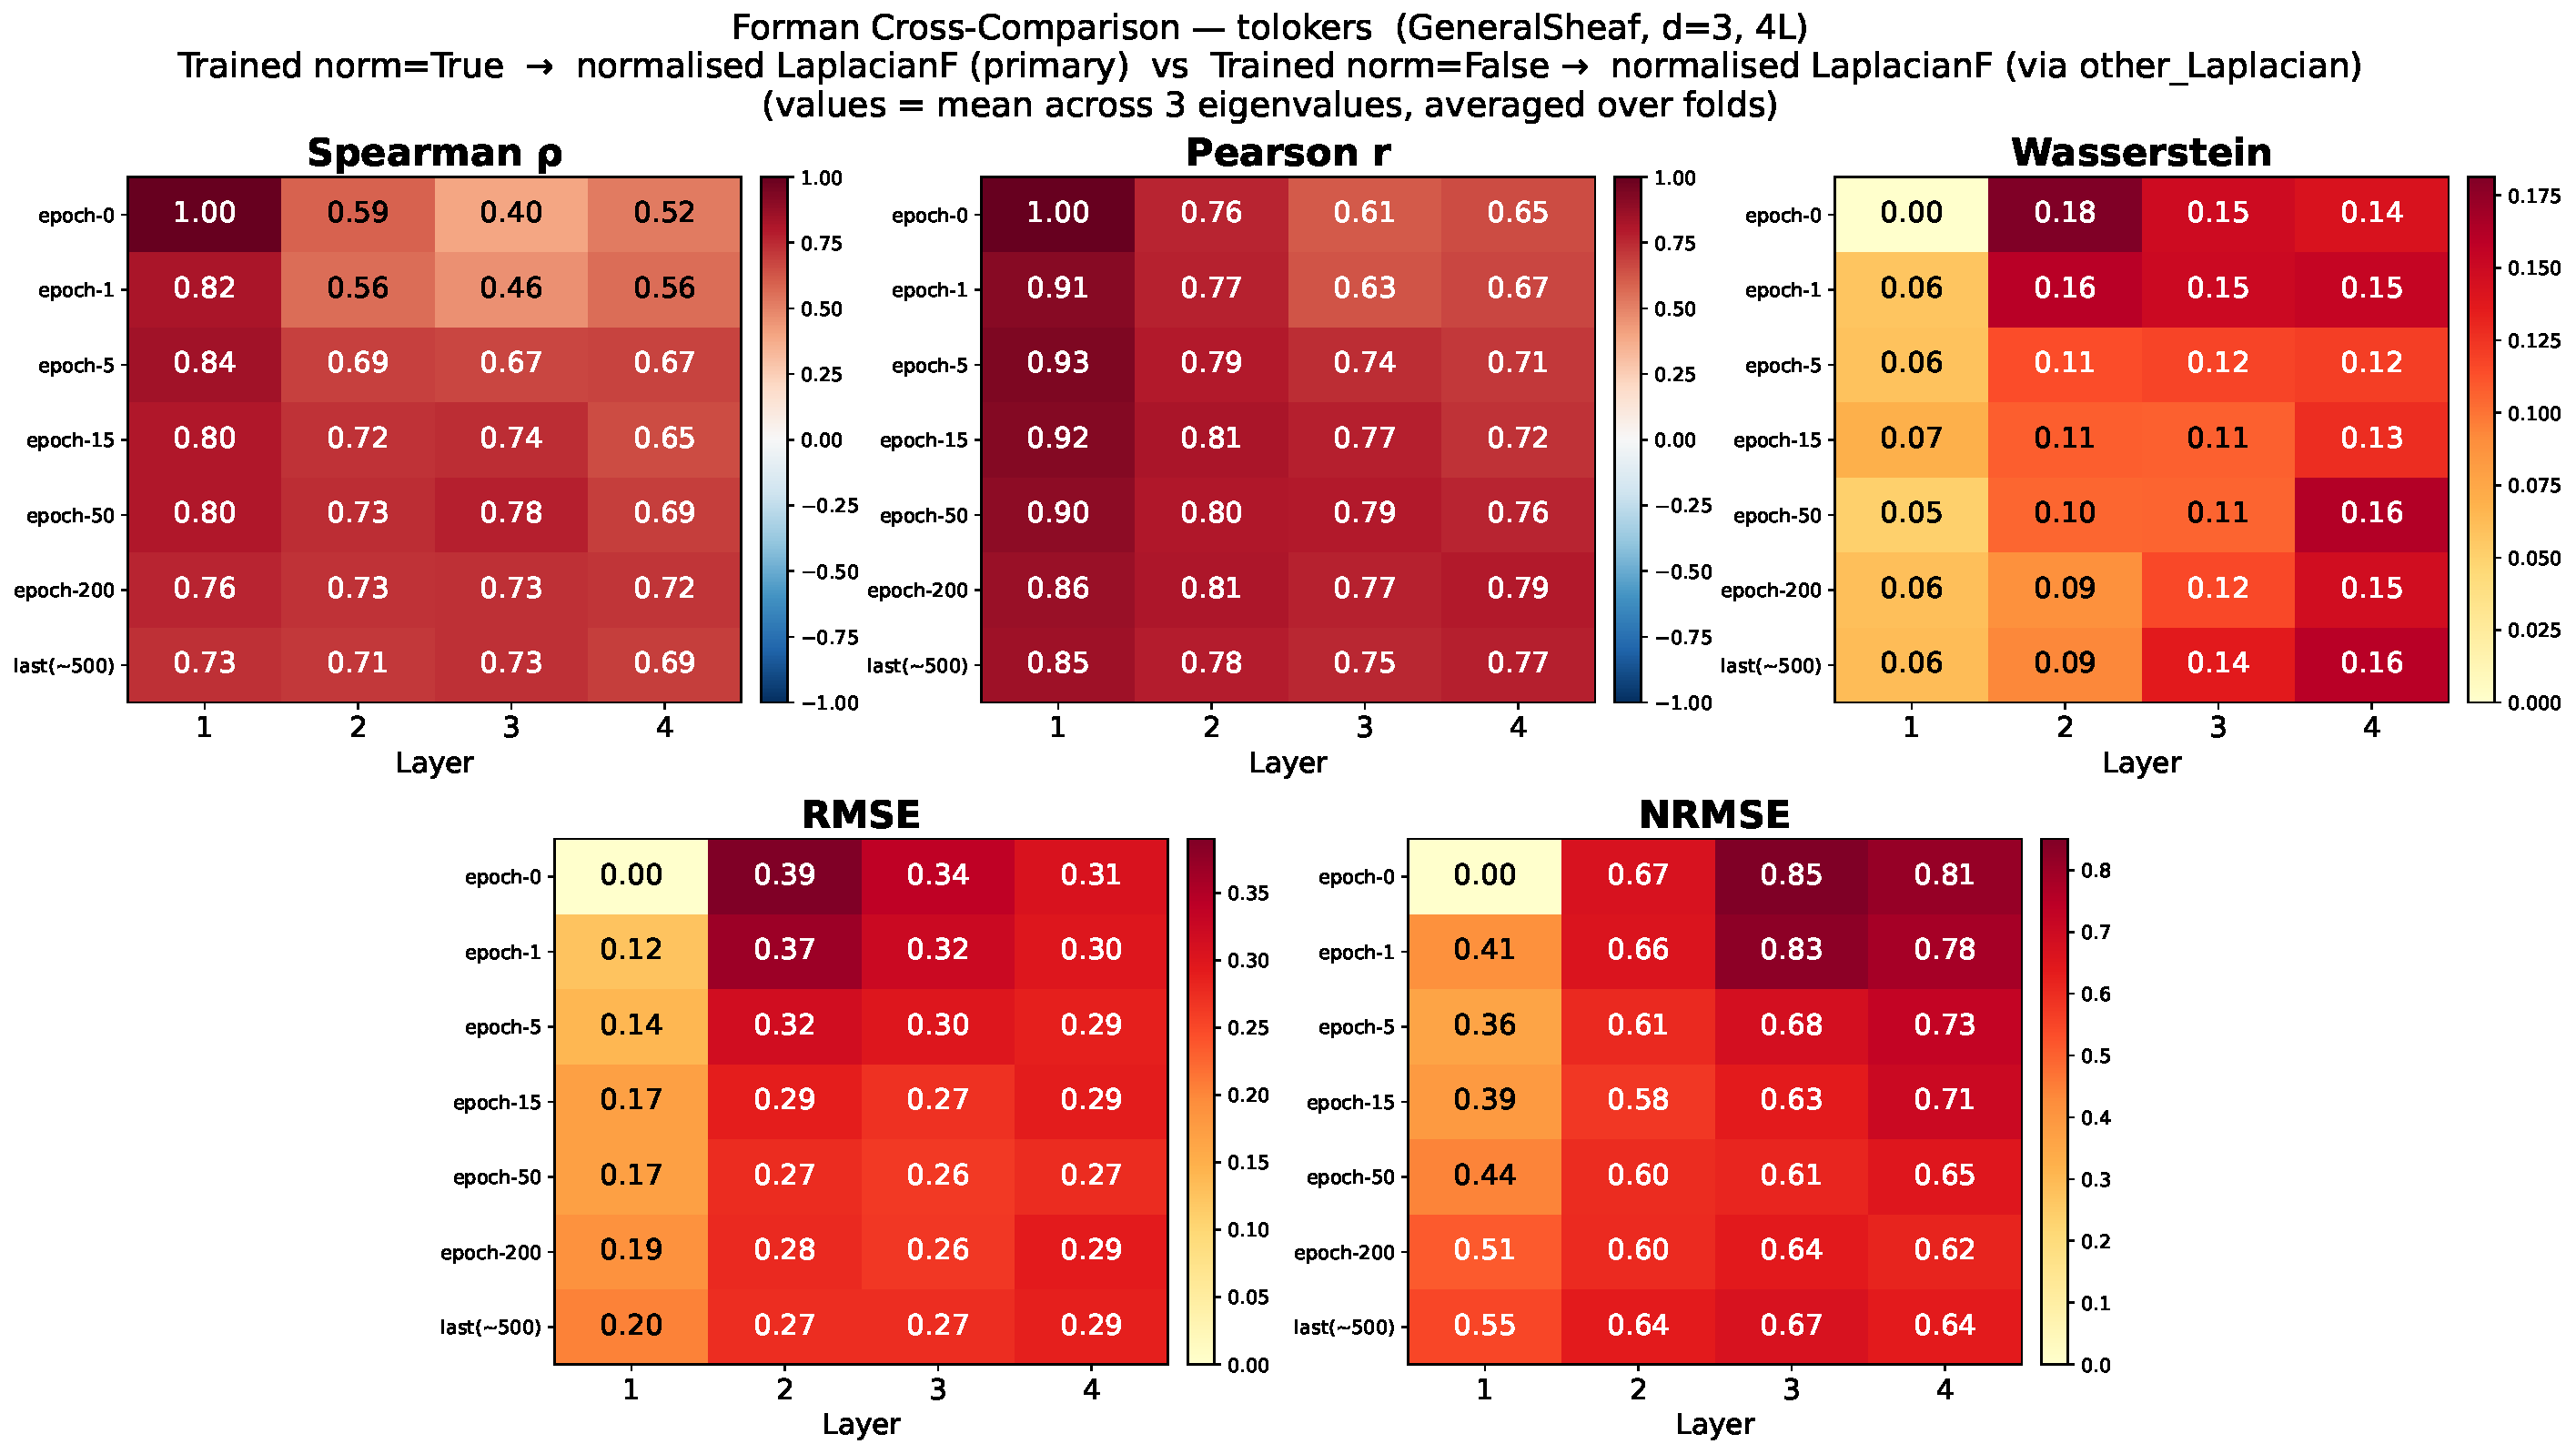
\includegraphics[width=\linewidth]{heatmaps/comparison/norm_true_vs_other_norm_false/tolokers_GeneralSheaf_d3_4L_norm_true_primary_vs_other_norm_false_heatmap.pdf}
\end{figure}
\end{frame}

\begin{frame}{Wisconsin --- Dir A: maps norm=True vs maps norm=False (both normalised $\widetilde{\Delta}_{\mathcal{F}}$)}
\begin{figure}
    \centering
    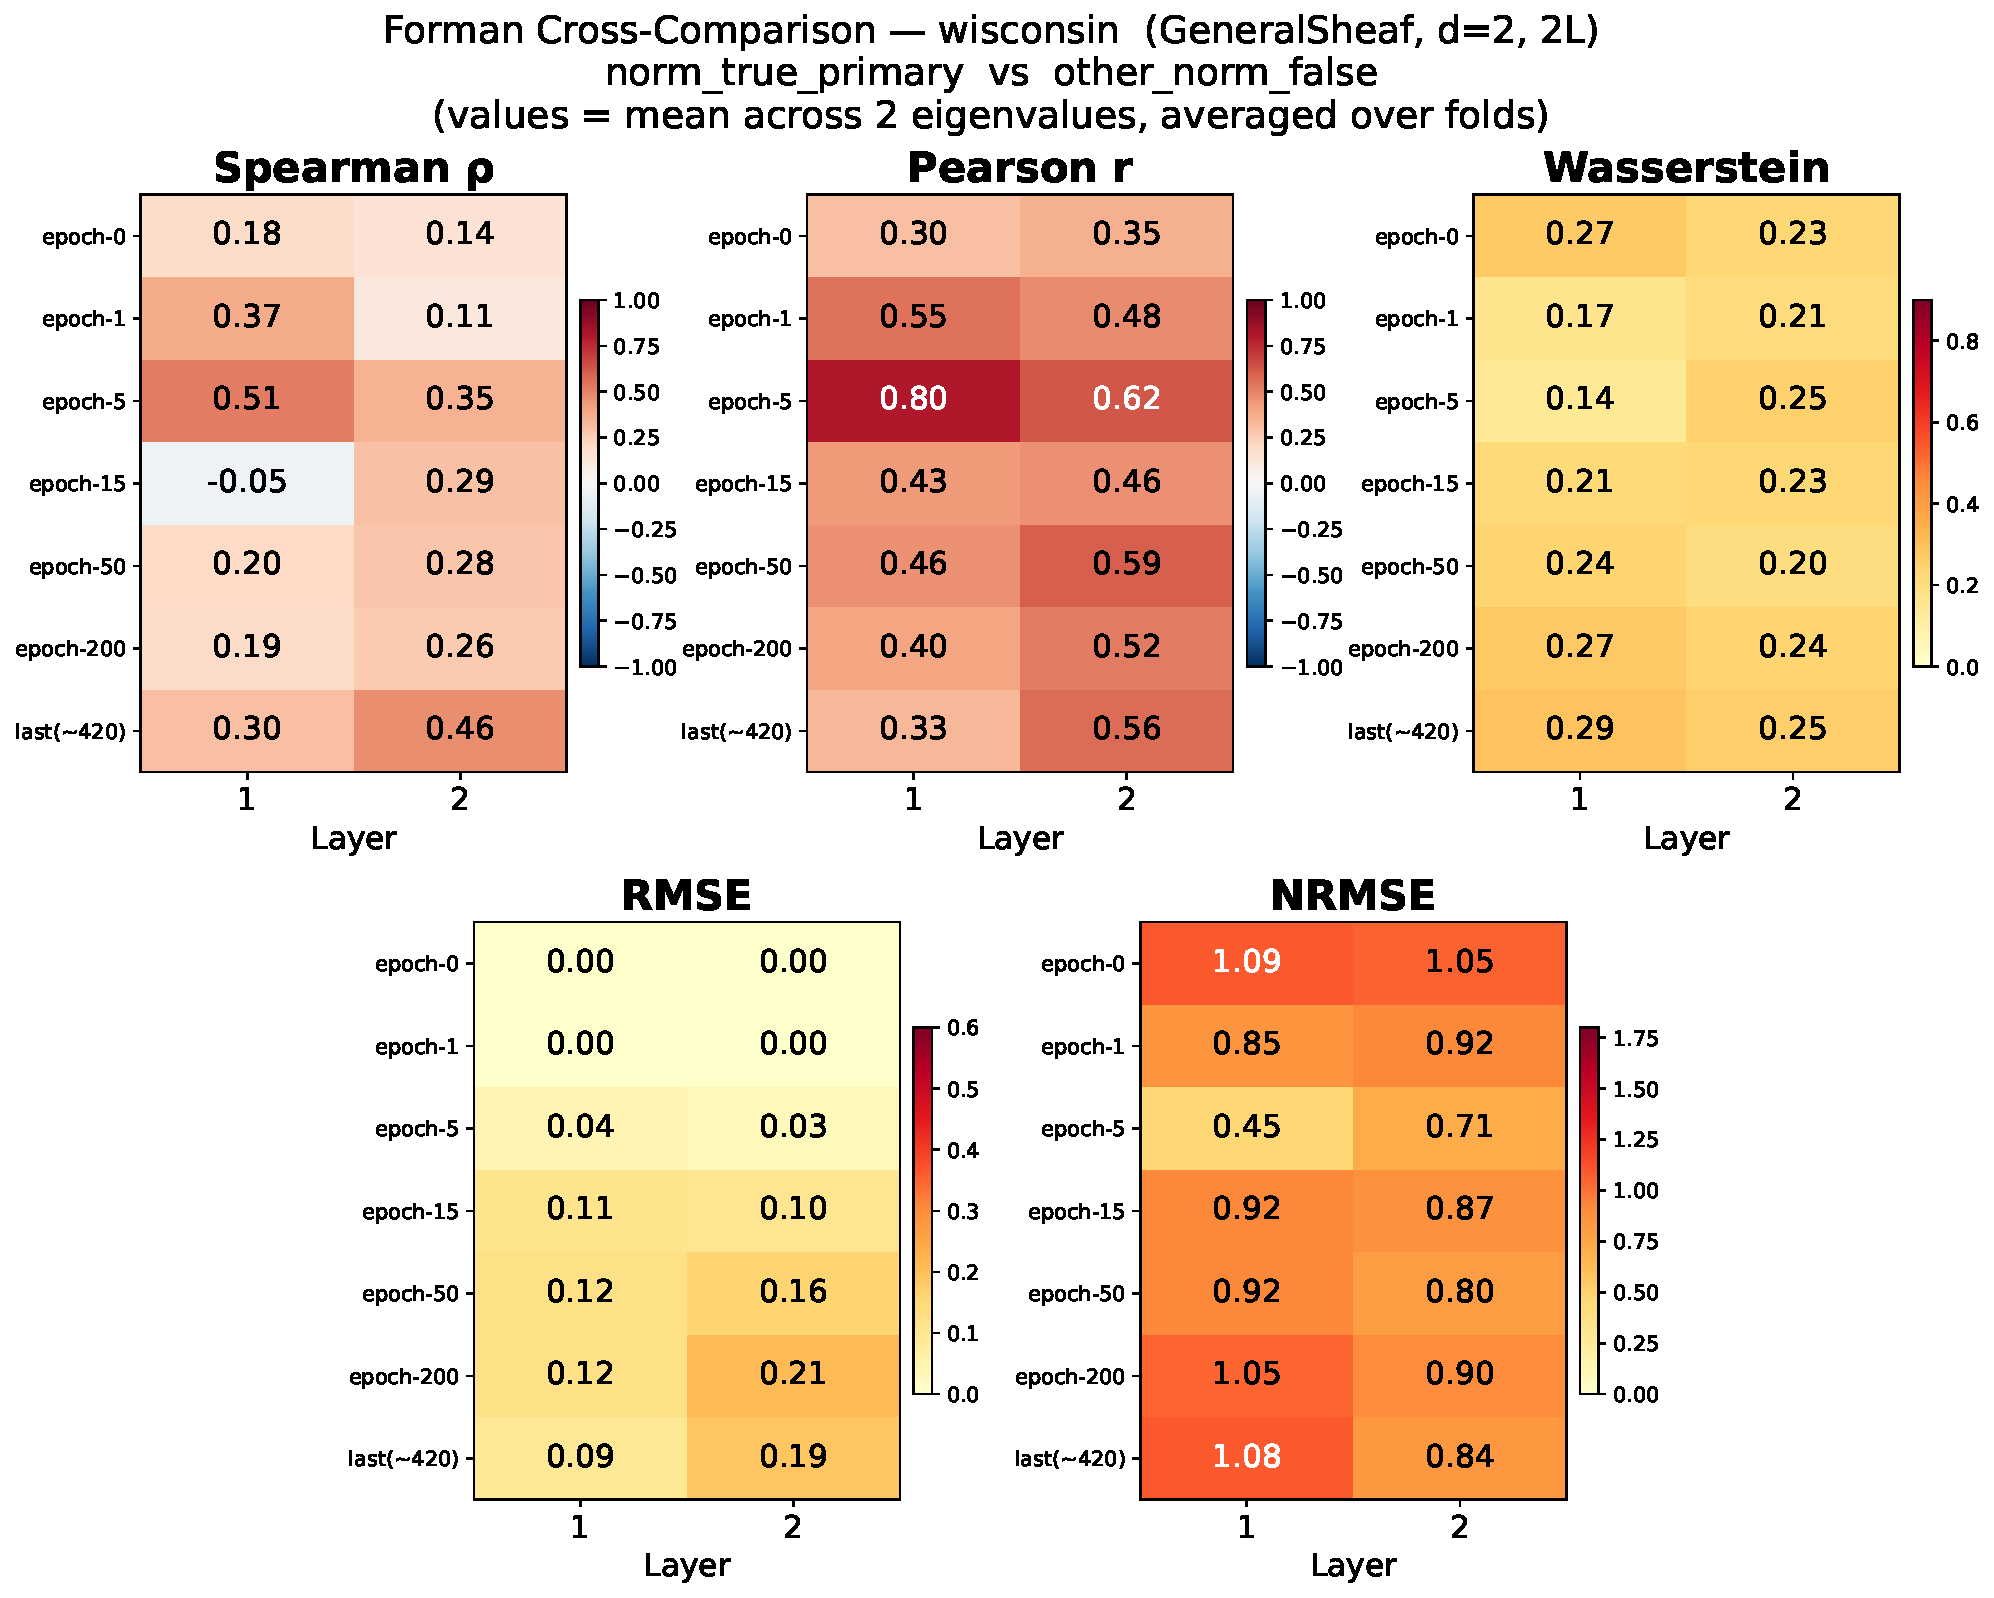
\includegraphics[width=\linewidth]{heatmaps/comparison/norm_true_vs_other_norm_false/wisconsin_GeneralSheaf_d2_2L_norm_true_primary_vs_other_norm_false_heatmap.pdf}
\end{figure}
\end{frame}

% ══════════════════════════════════════════════════════════════════════════════
%  SECTION 4 — Cross-comparison Direction B: both unnormalised, different training objectives
% ══════════════════════════════════════════════════════════════════════════════

\begin{frame}{}
\centering
\Huge\textbf{Cross-Comparison --- Direction B}\\[6pt]
\Large Both profiles: unnormalised $\Delta_{\mathcal{F}}$\\[4pt]
\large Maps from \texttt{norm=False} training \textbf{vs} maps from \texttt{norm=True} training\\[4pt]
\normalsize (same Laplacian normalisation, different training objective)
\end{frame}

\begin{frame}{Amazon Ratings --- Dir B: maps norm=False vs maps norm=True (both unnorm. $\Delta_{\mathcal{F}}$)}
\begin{figure}
    \centering
    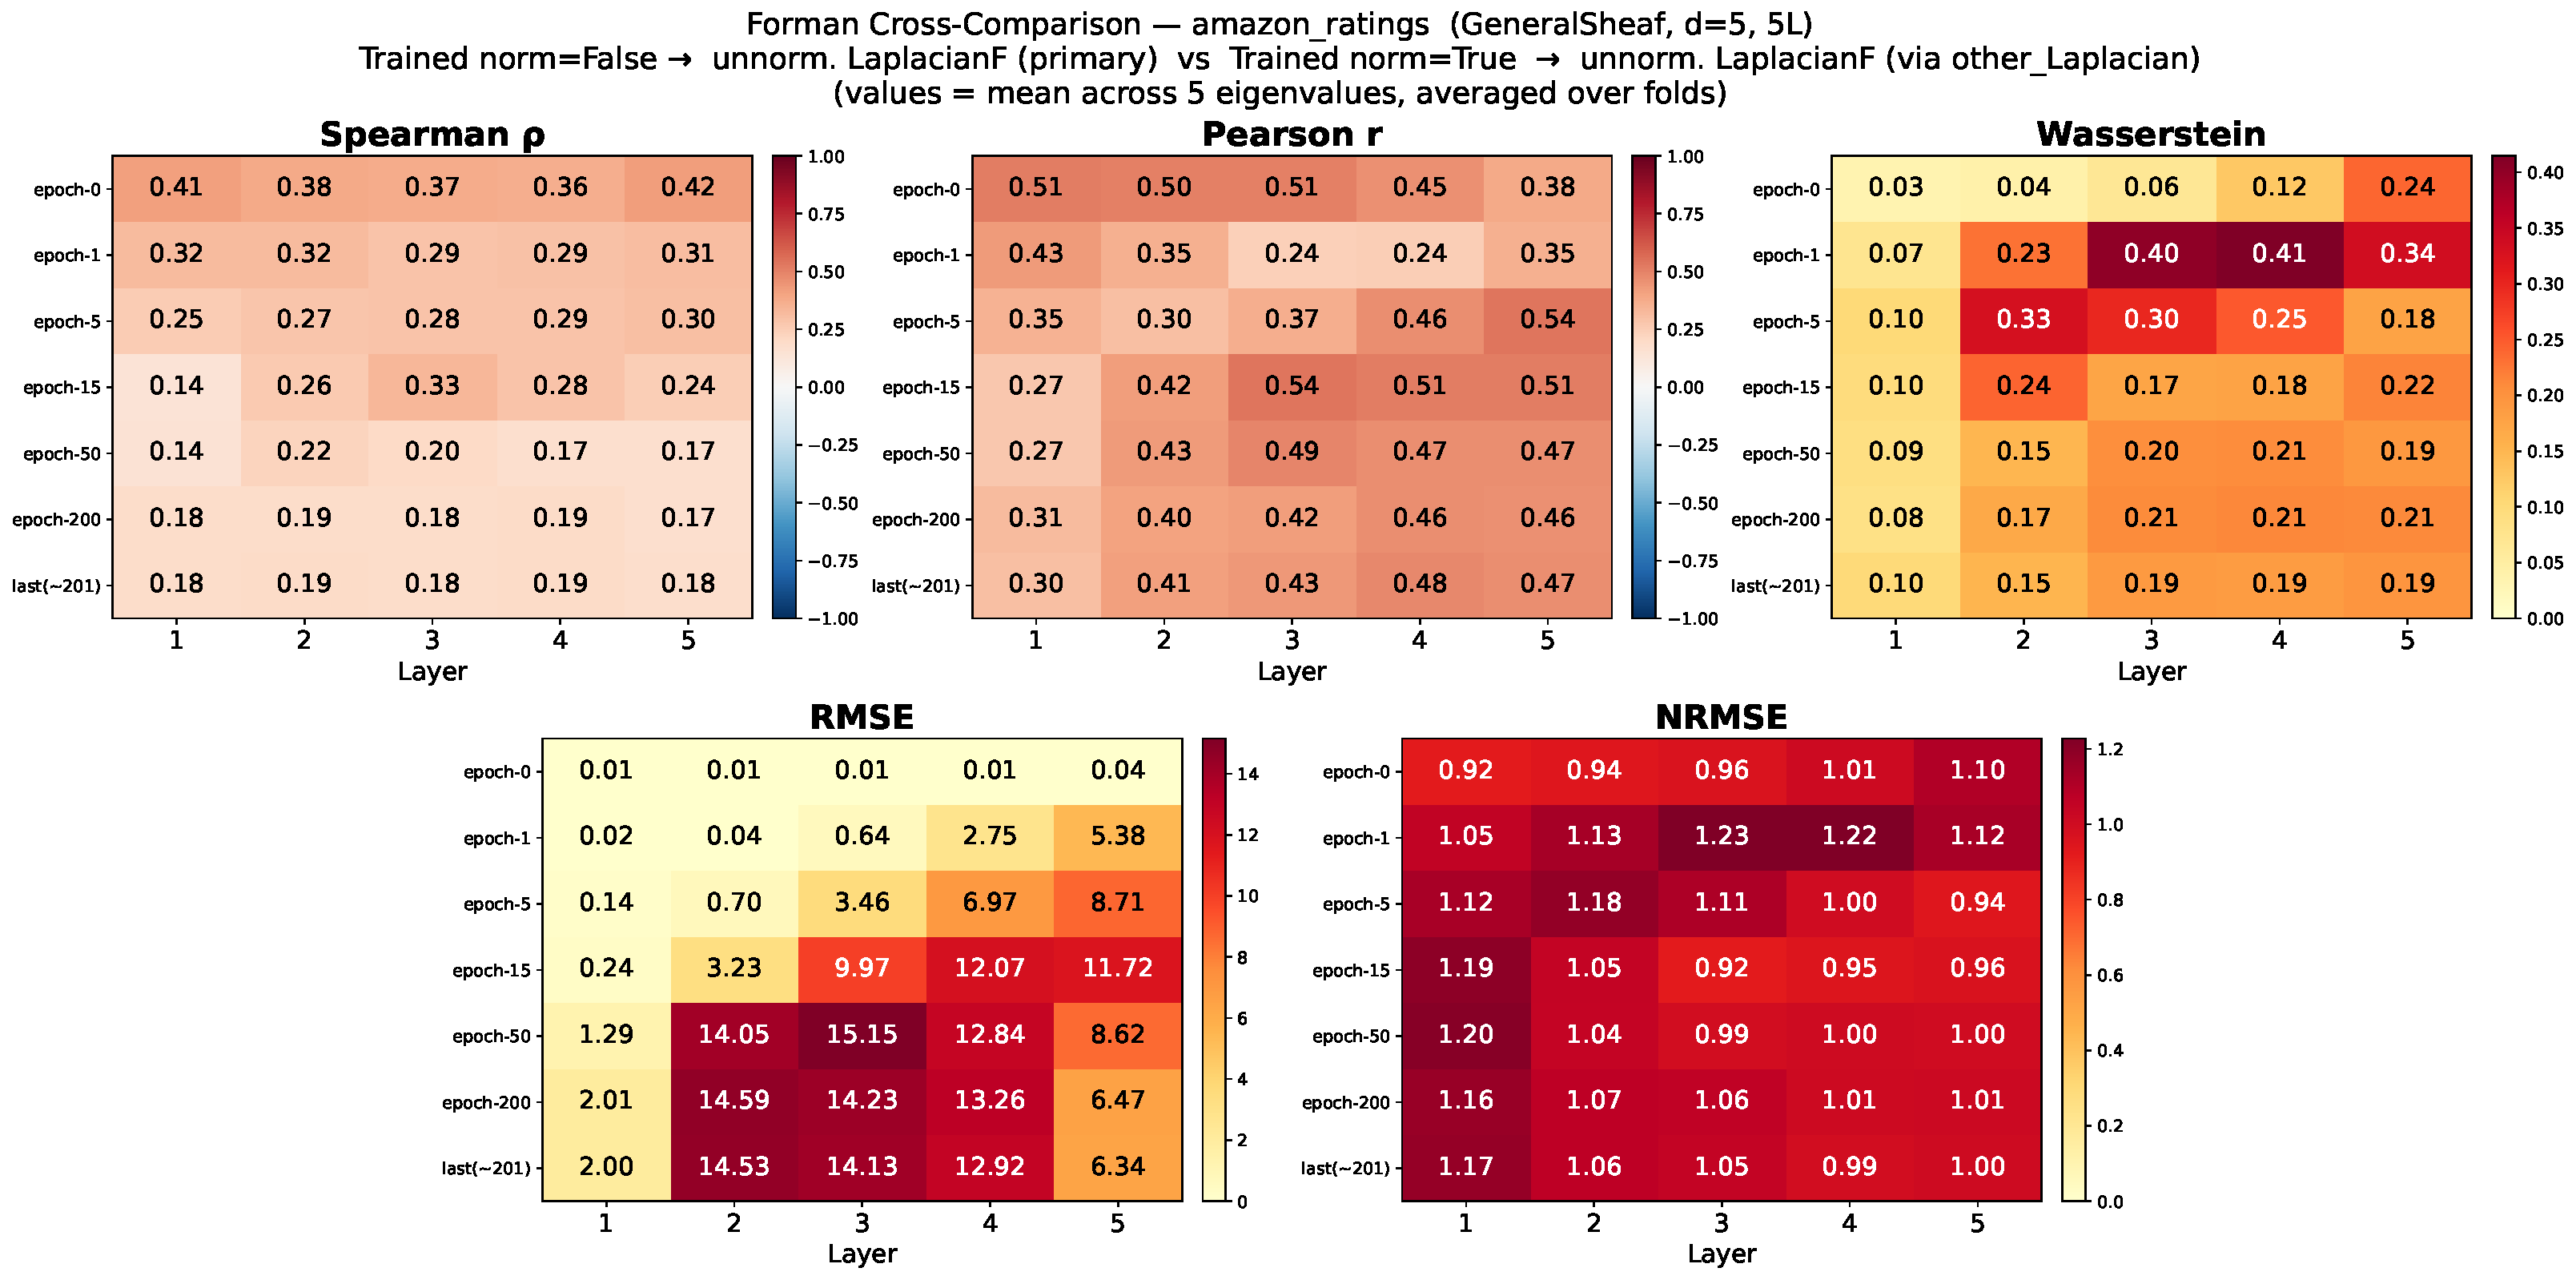
\includegraphics[width=\linewidth]{heatmaps/comparison/norm_false_vs_other_norm_true/amazon_ratings_GeneralSheaf_d5_5L_norm_false_primary_vs_other_norm_true_heatmap.pdf}
\end{figure}
\end{frame}

\begin{frame}{Citeseer --- Dir B: maps norm=False vs maps norm=True (both unnorm. $\Delta_{\mathcal{F}}$)}
\begin{figure}
    \centering
    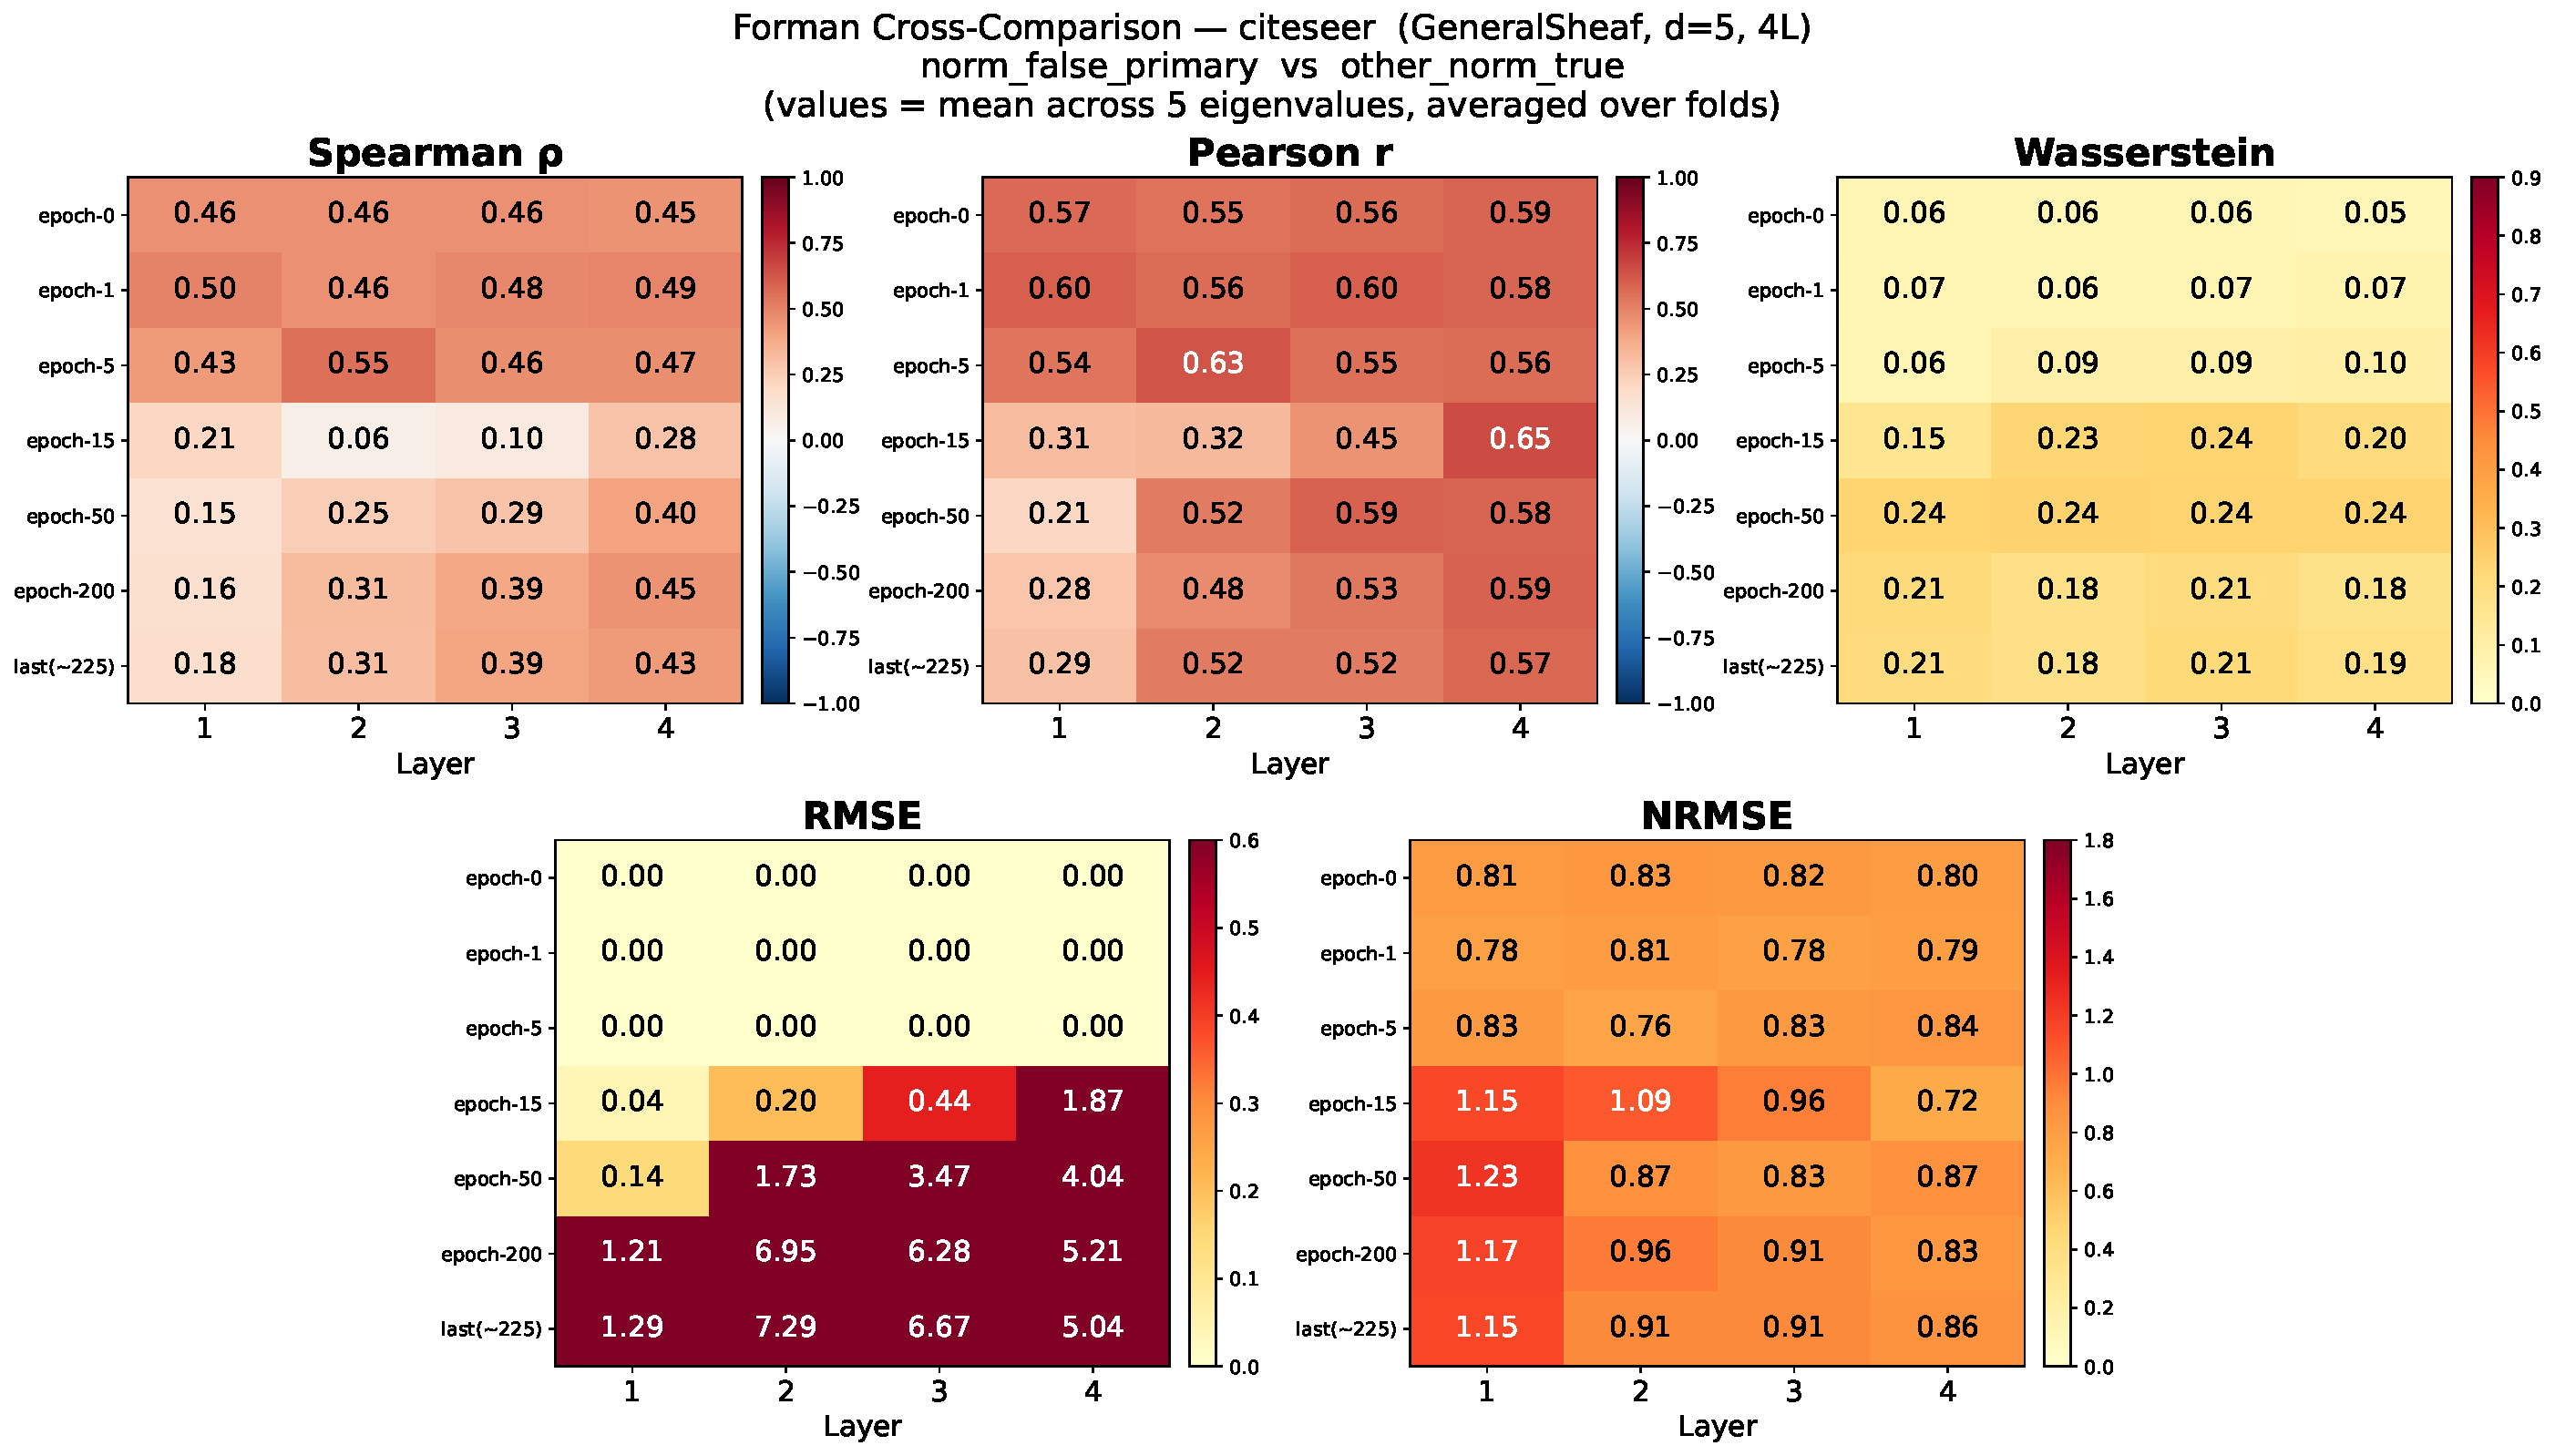
\includegraphics[width=\linewidth]{heatmaps/comparison/norm_false_vs_other_norm_true/citeseer_GeneralSheaf_d5_4L_norm_false_primary_vs_other_norm_true_heatmap.pdf}
\end{figure}
\end{frame}

\begin{frame}{Cora --- Dir B: maps norm=False vs maps norm=True (both unnorm. $\Delta_{\mathcal{F}}$)}
\begin{figure}
    \centering
    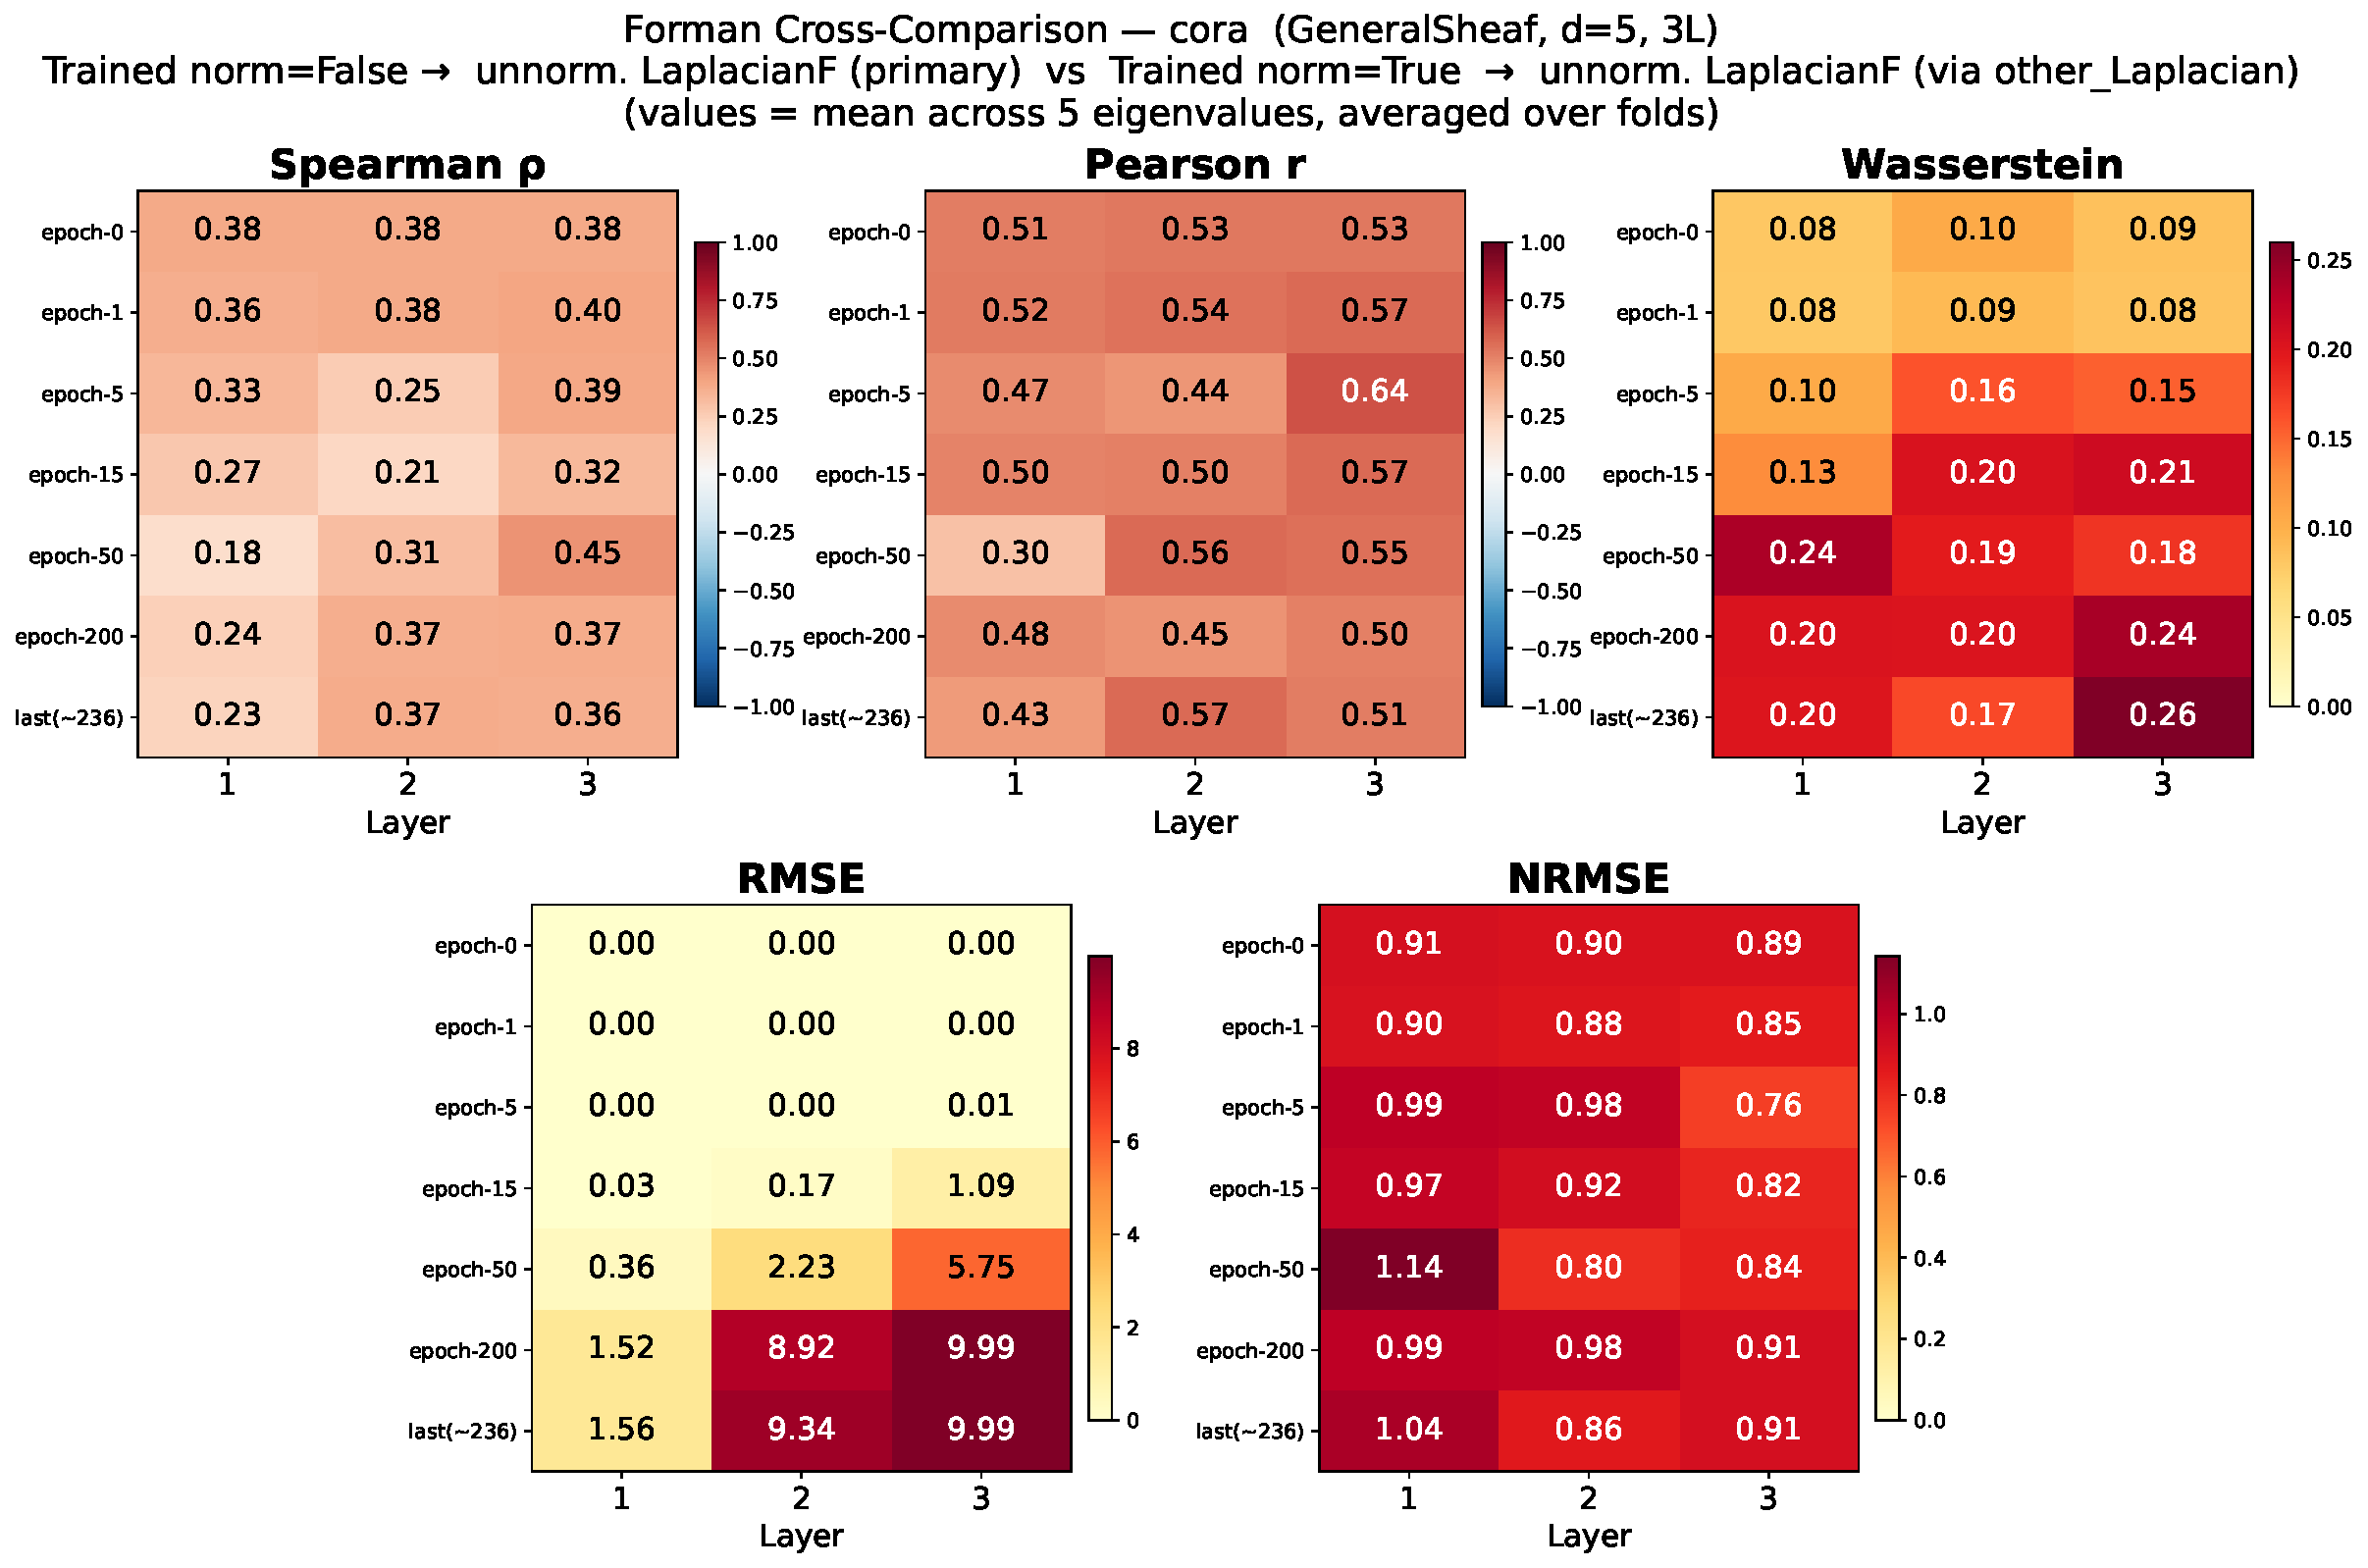
\includegraphics[width=\linewidth]{heatmaps/comparison/norm_false_vs_other_norm_true/cora_GeneralSheaf_d5_3L_norm_false_primary_vs_other_norm_true_heatmap.pdf}
\end{figure}
\end{frame}

\begin{frame}{Cornell --- Dir B: maps norm=False vs maps norm=True (both unnorm. $\Delta_{\mathcal{F}}$)}
\begin{figure}
    \centering
    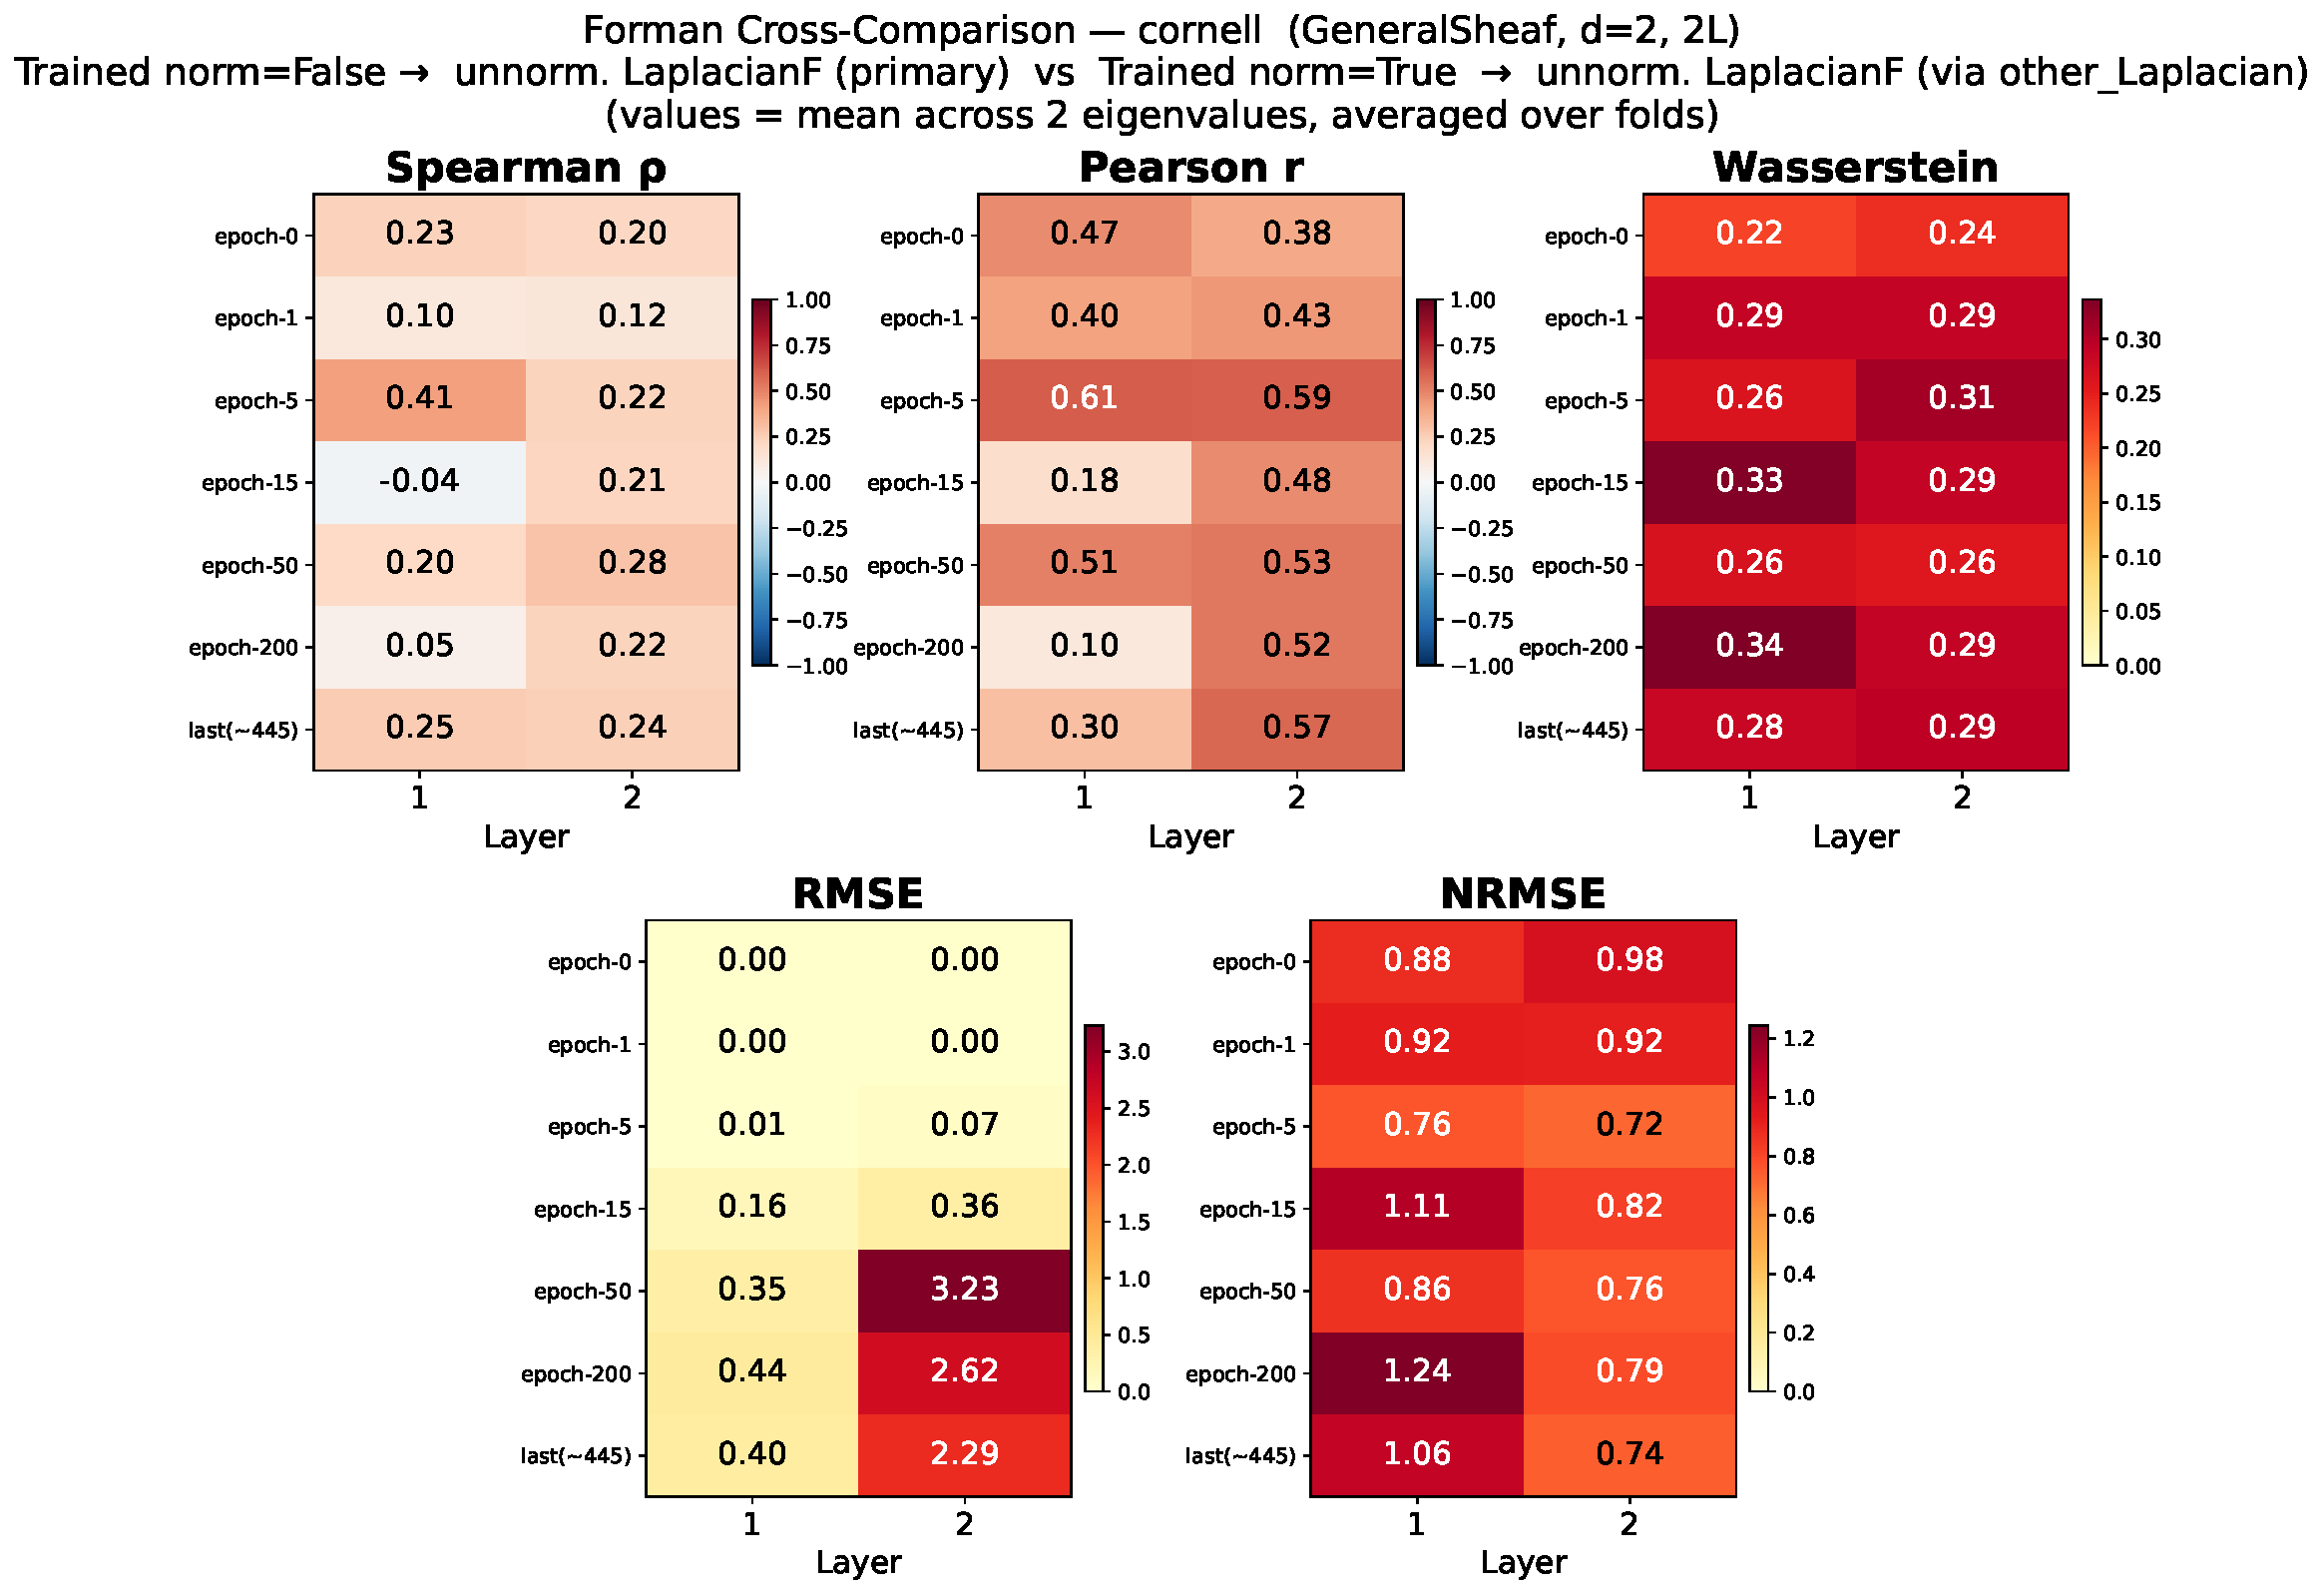
\includegraphics[width=\linewidth]{heatmaps/comparison/norm_false_vs_other_norm_true/cornell_GeneralSheaf_d2_2L_norm_false_primary_vs_other_norm_true_heatmap.pdf}
\end{figure}
\end{frame}

\begin{frame}{Minesweeper --- Dir B: maps norm=False vs maps norm=True (both unnorm. $\Delta_{\mathcal{F}}$)}
\begin{figure}
    \centering
    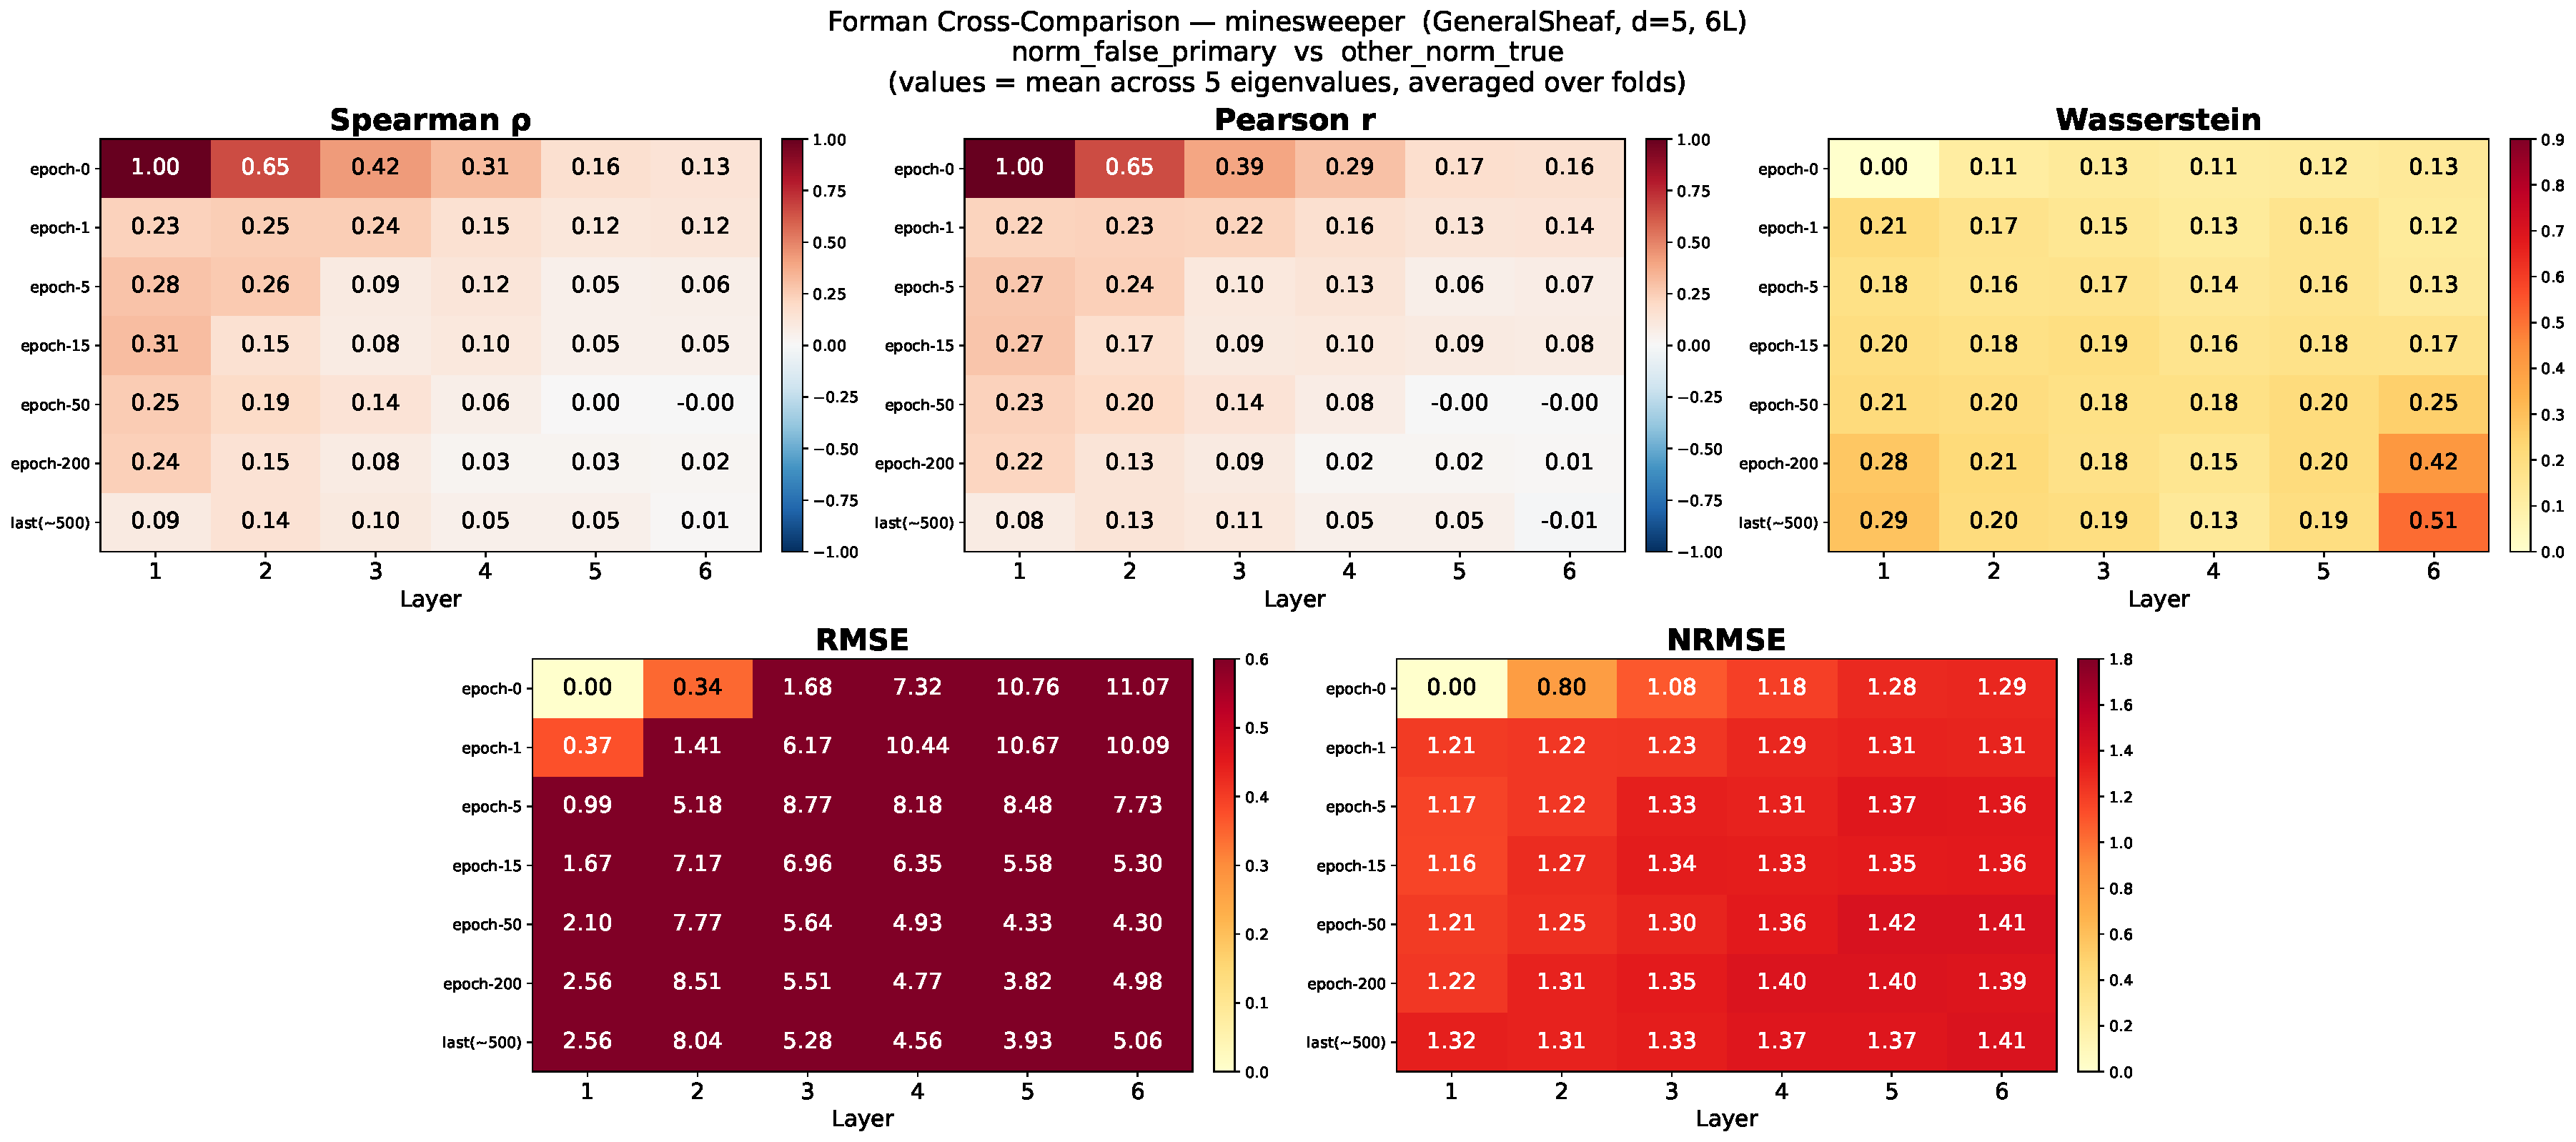
\includegraphics[width=\linewidth]{heatmaps/comparison/norm_false_vs_other_norm_true/minesweeper_GeneralSheaf_d5_6L_norm_false_primary_vs_other_norm_true_heatmap.pdf}
\end{figure}
\end{frame}

\begin{frame}{Pubmed --- Dir B: maps norm=False vs maps norm=True (both unnorm. $\Delta_{\mathcal{F}}$)}
\begin{figure}
    \centering
    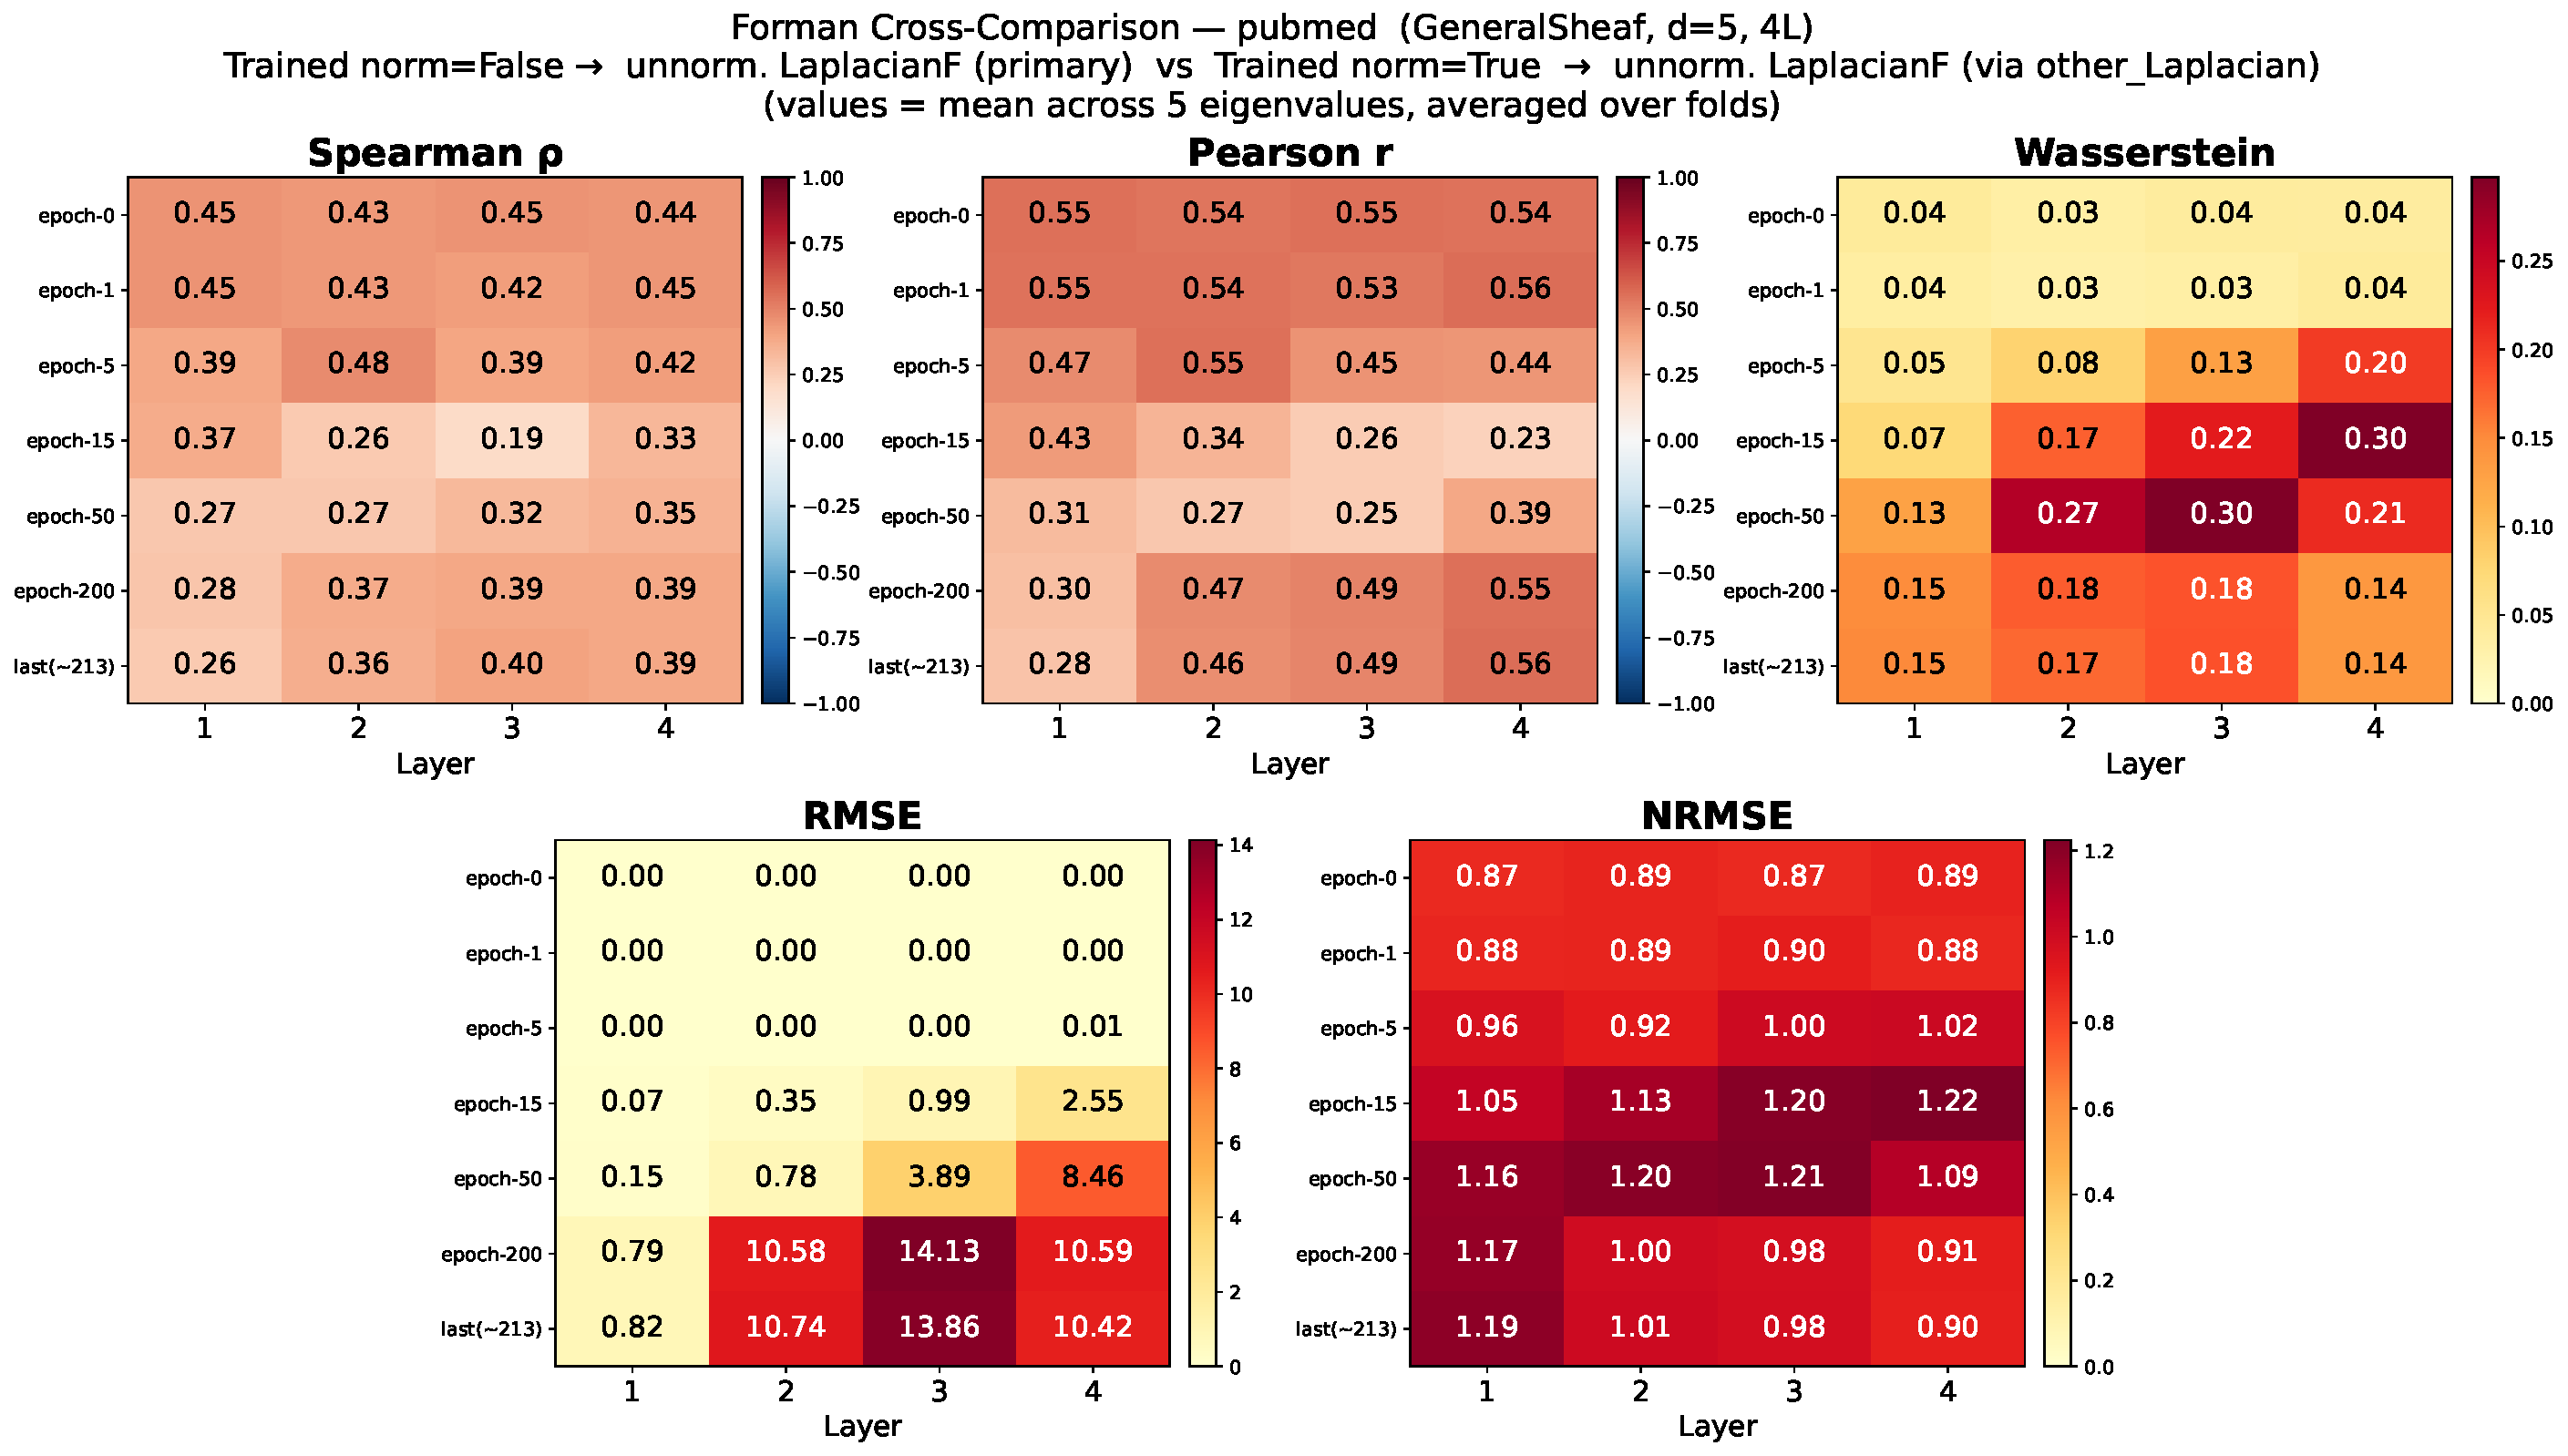
\includegraphics[width=\linewidth]{heatmaps/comparison/norm_false_vs_other_norm_true/pubmed_GeneralSheaf_d5_4L_norm_false_primary_vs_other_norm_true_heatmap.pdf}
\end{figure}
\end{frame}

\begin{frame}{Questions --- Dir B: maps norm=False vs maps norm=True (both unnorm. $\Delta_{\mathcal{F}}$)}
\begin{figure}
    \centering
    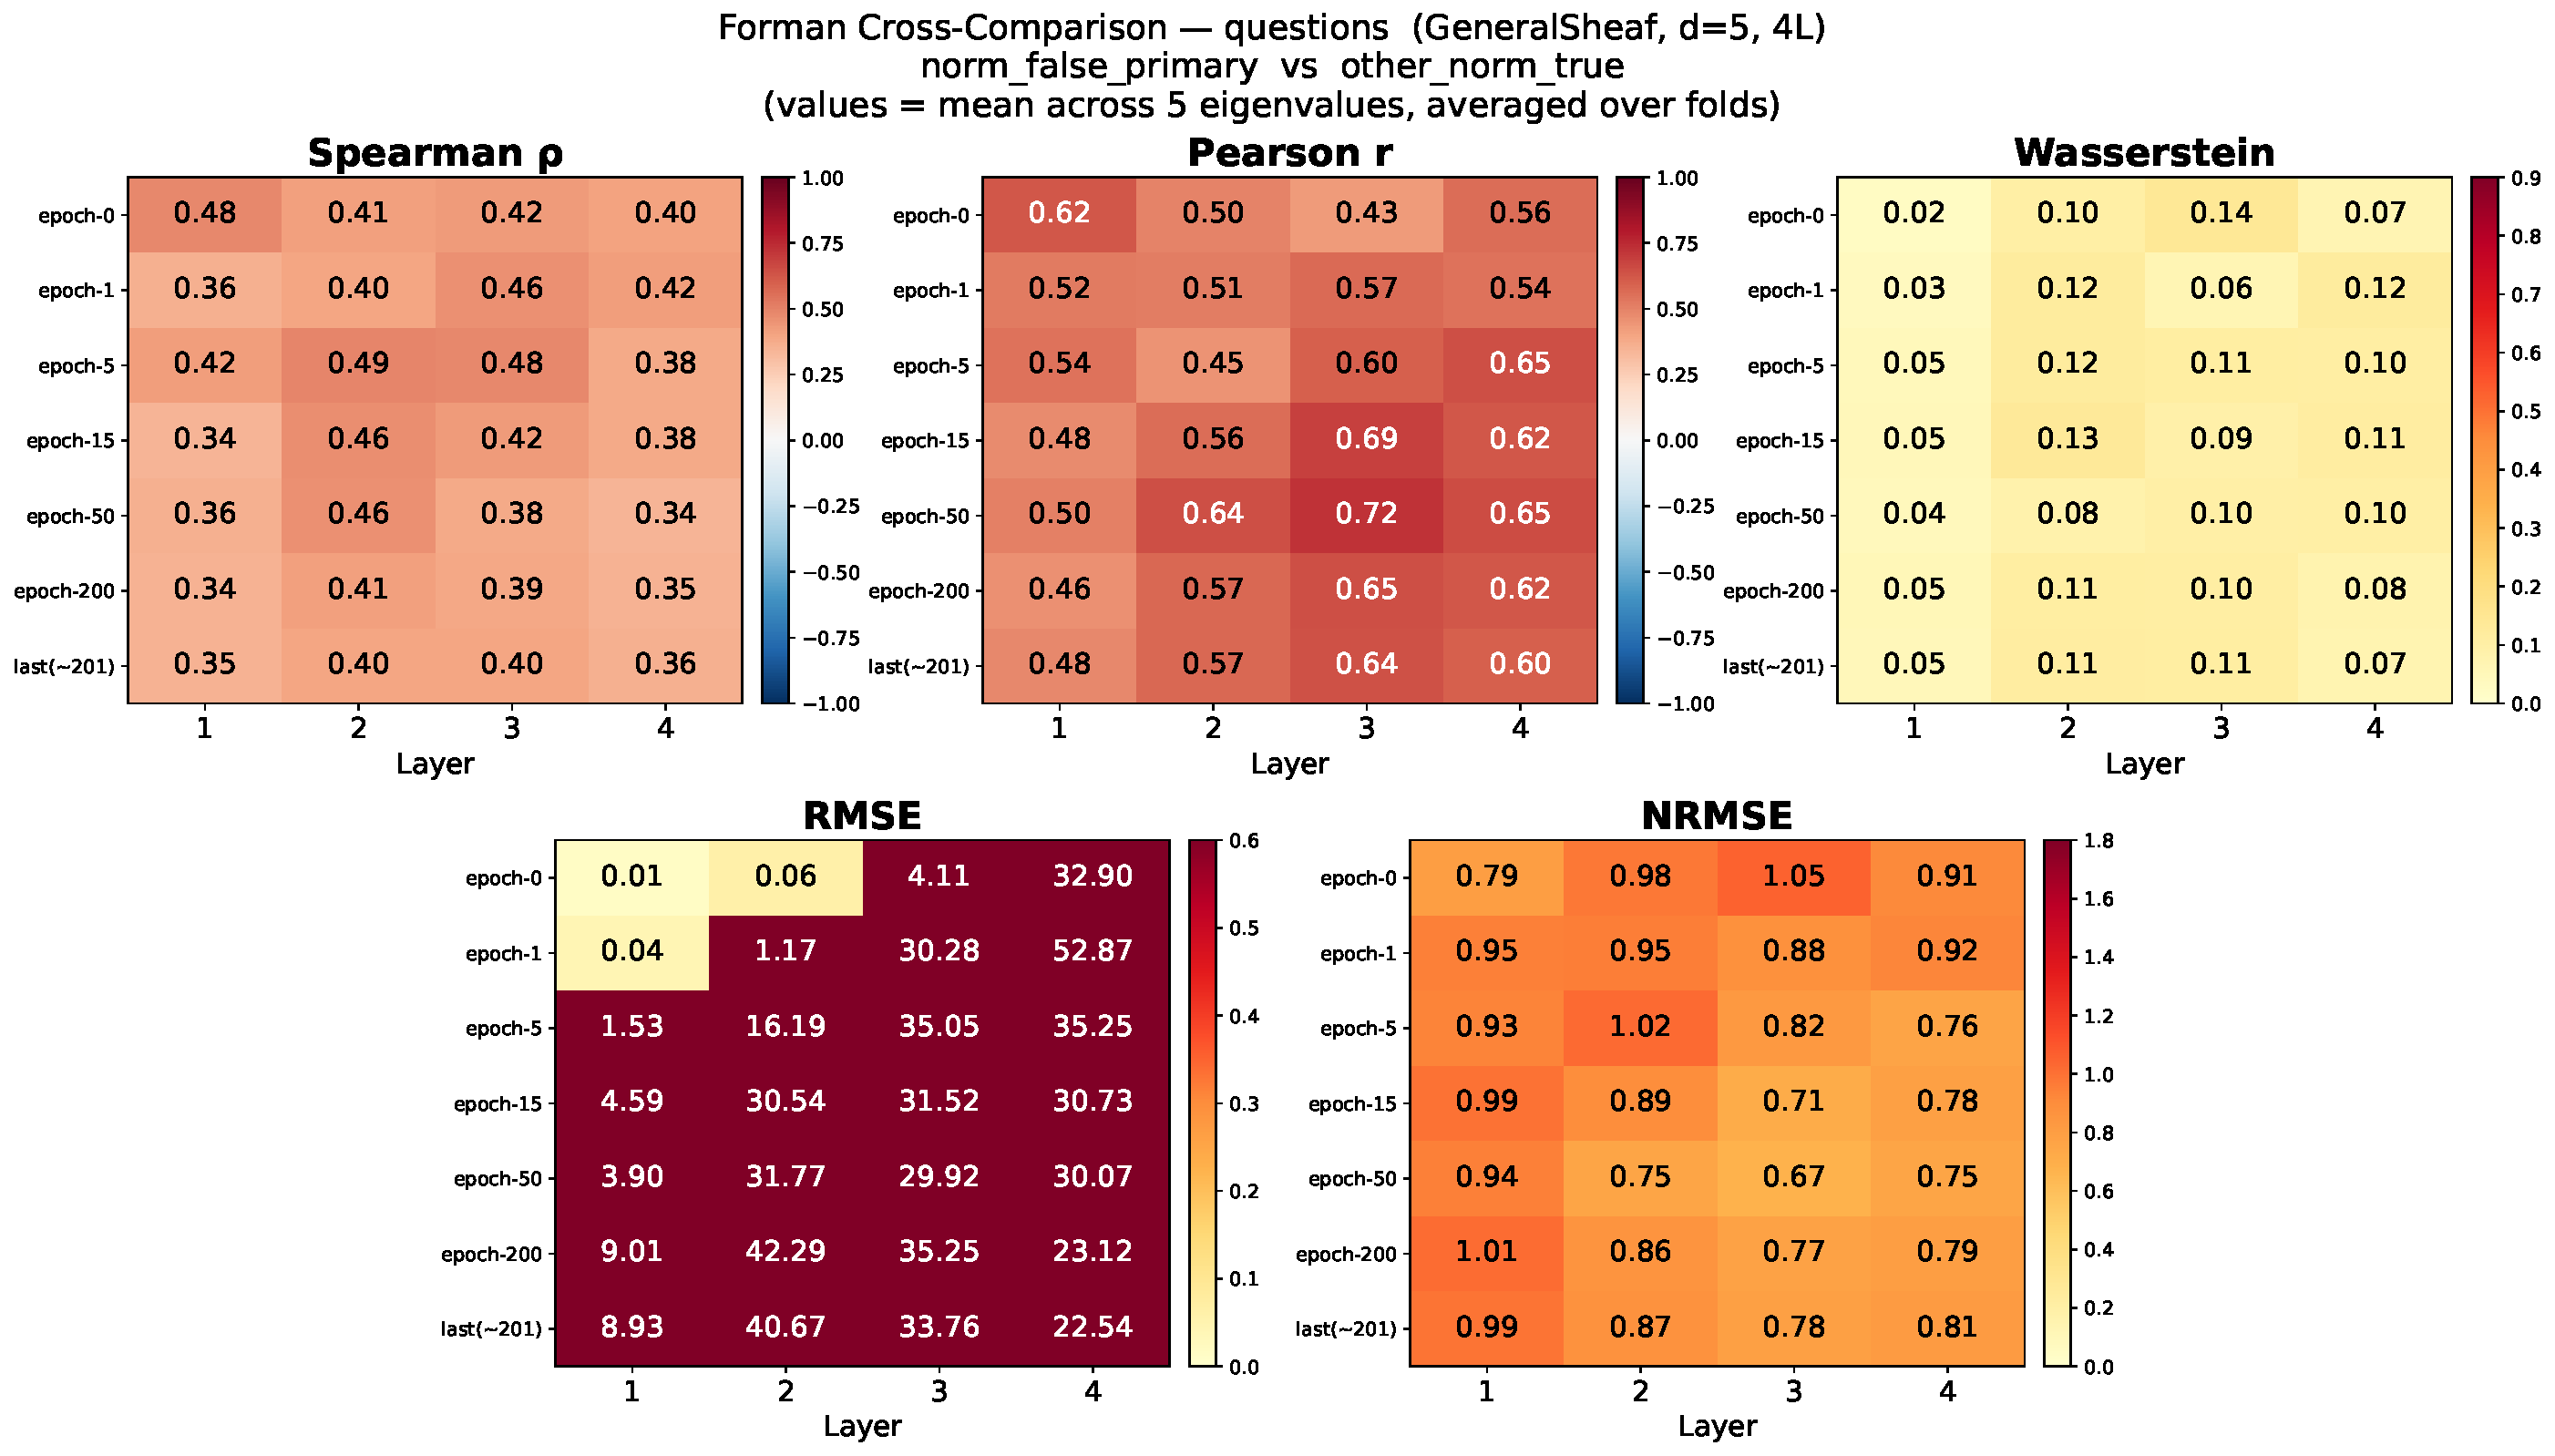
\includegraphics[width=\linewidth]{heatmaps/comparison/norm_false_vs_other_norm_true/questions_GeneralSheaf_d5_4L_norm_false_primary_vs_other_norm_true_heatmap.pdf}
\end{figure}
\end{frame}

\begin{frame}{Roman Empire --- Dir B: maps norm=False vs maps norm=True (both unnorm. $\Delta_{\mathcal{F}}$)}
\begin{figure}
    \centering
    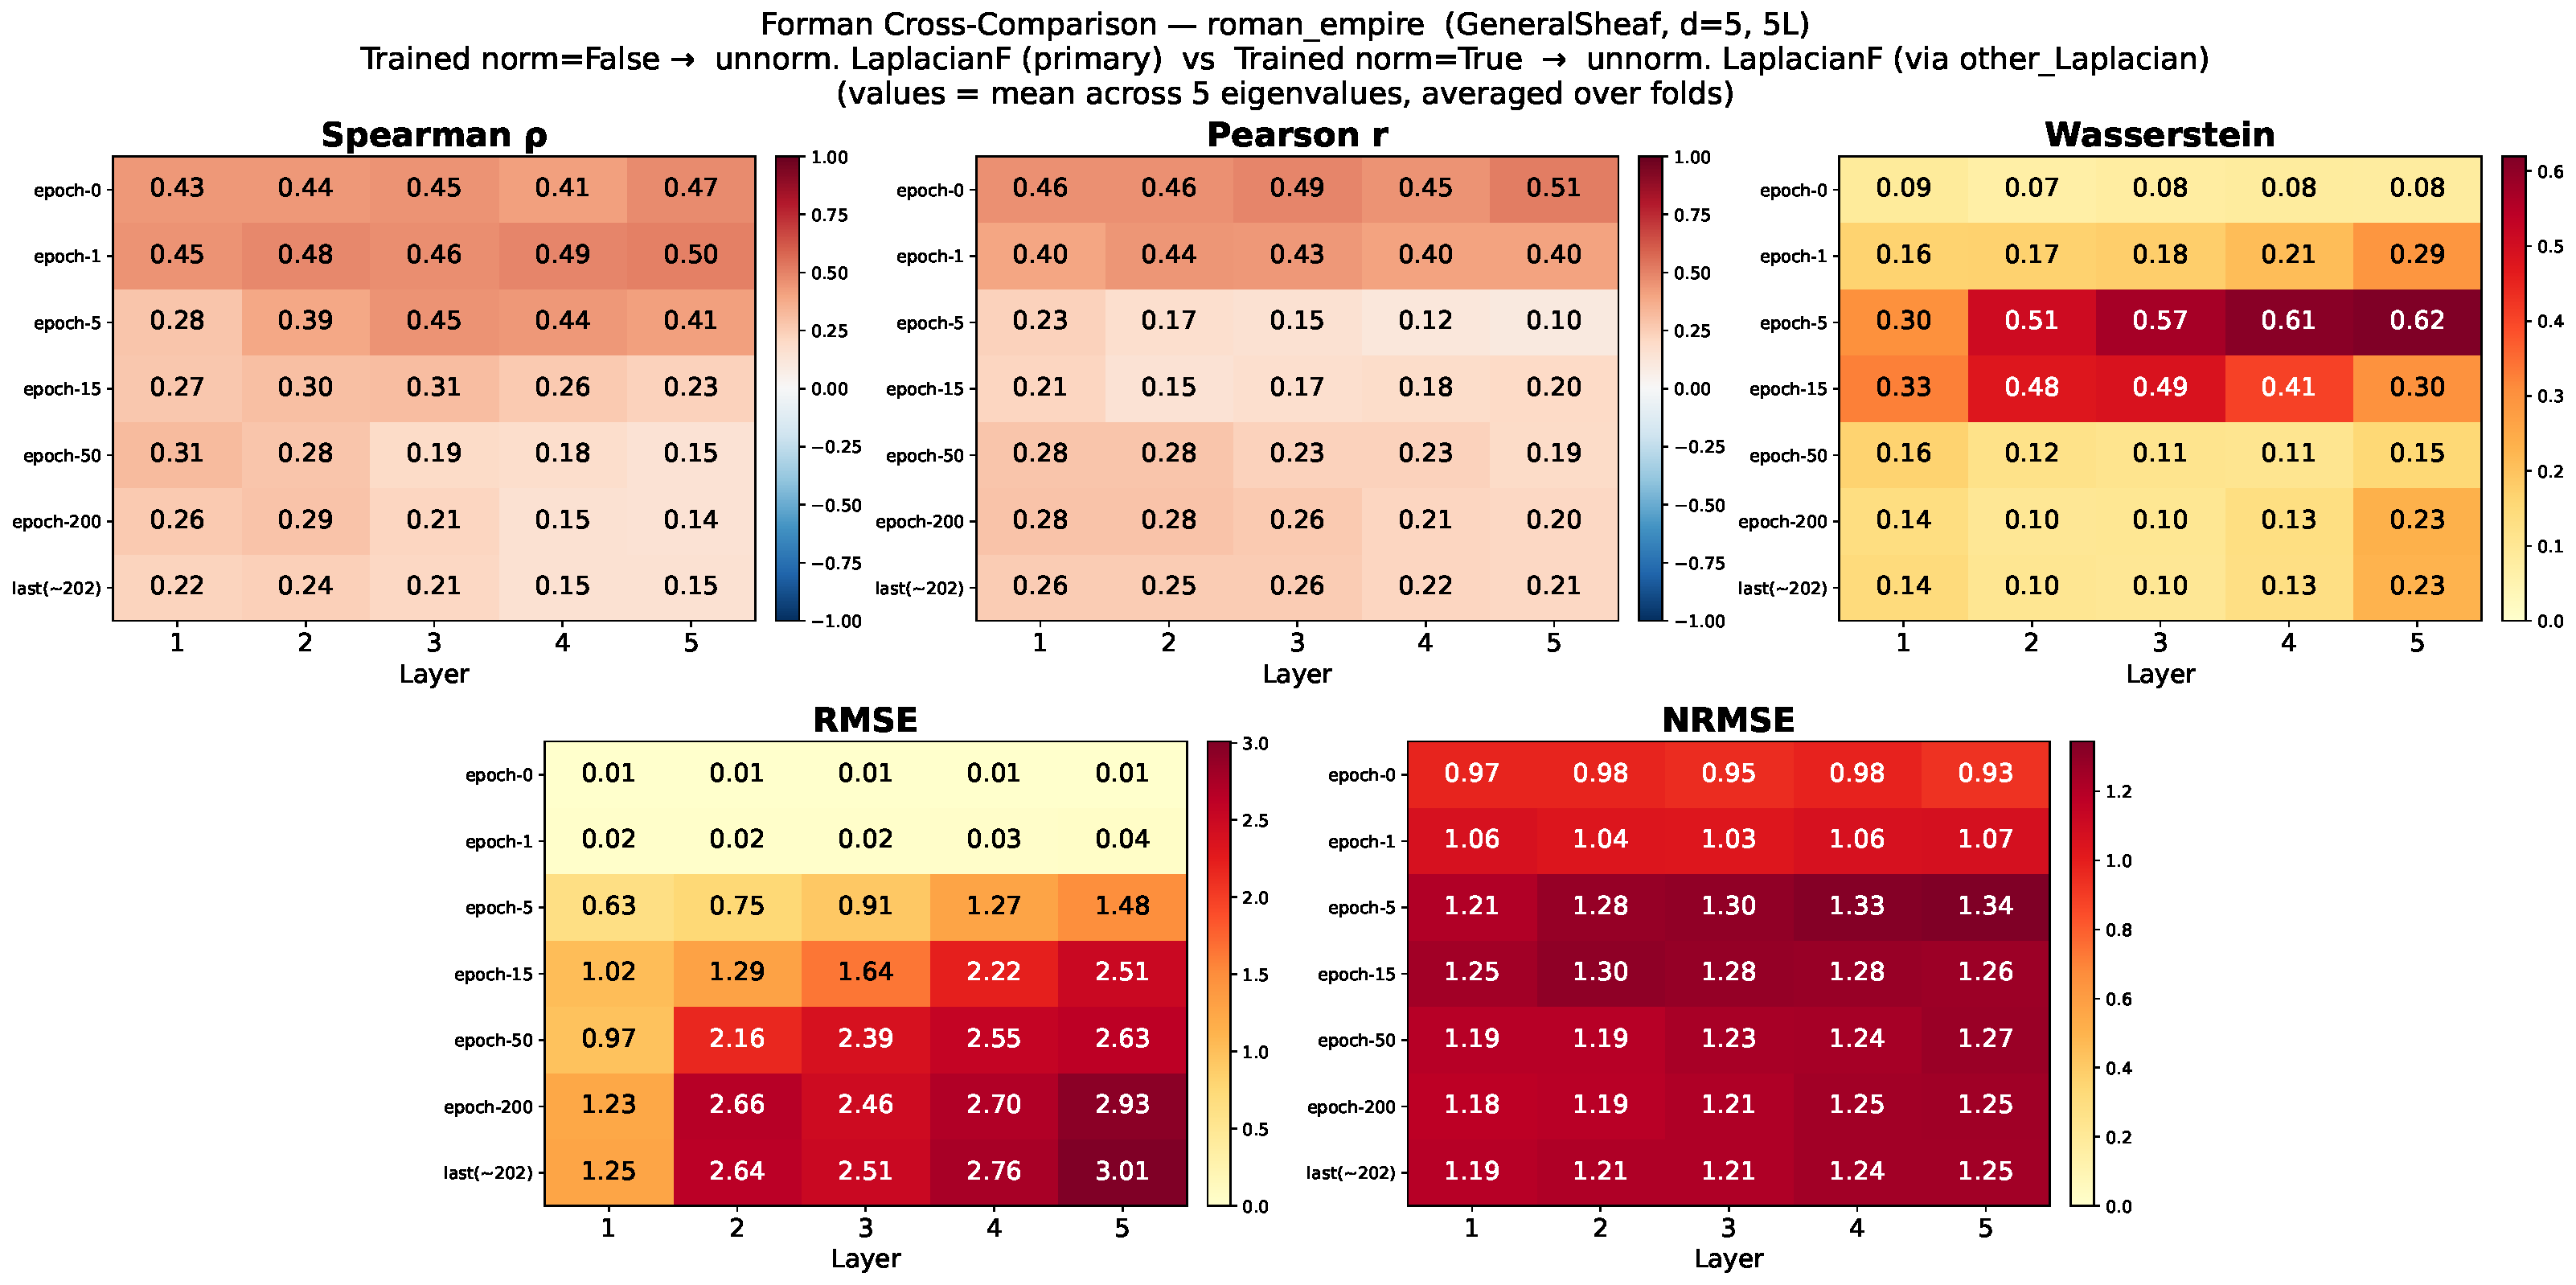
\includegraphics[width=\linewidth]{heatmaps/comparison/norm_false_vs_other_norm_true/roman_empire_GeneralSheaf_d5_5L_norm_false_primary_vs_other_norm_true_heatmap.pdf}
\end{figure}
\end{frame}

\begin{frame}{Tolokers --- Dir B: maps norm=False vs maps norm=True (both unnorm. $\Delta_{\mathcal{F}}$)}
\begin{figure}
    \centering
    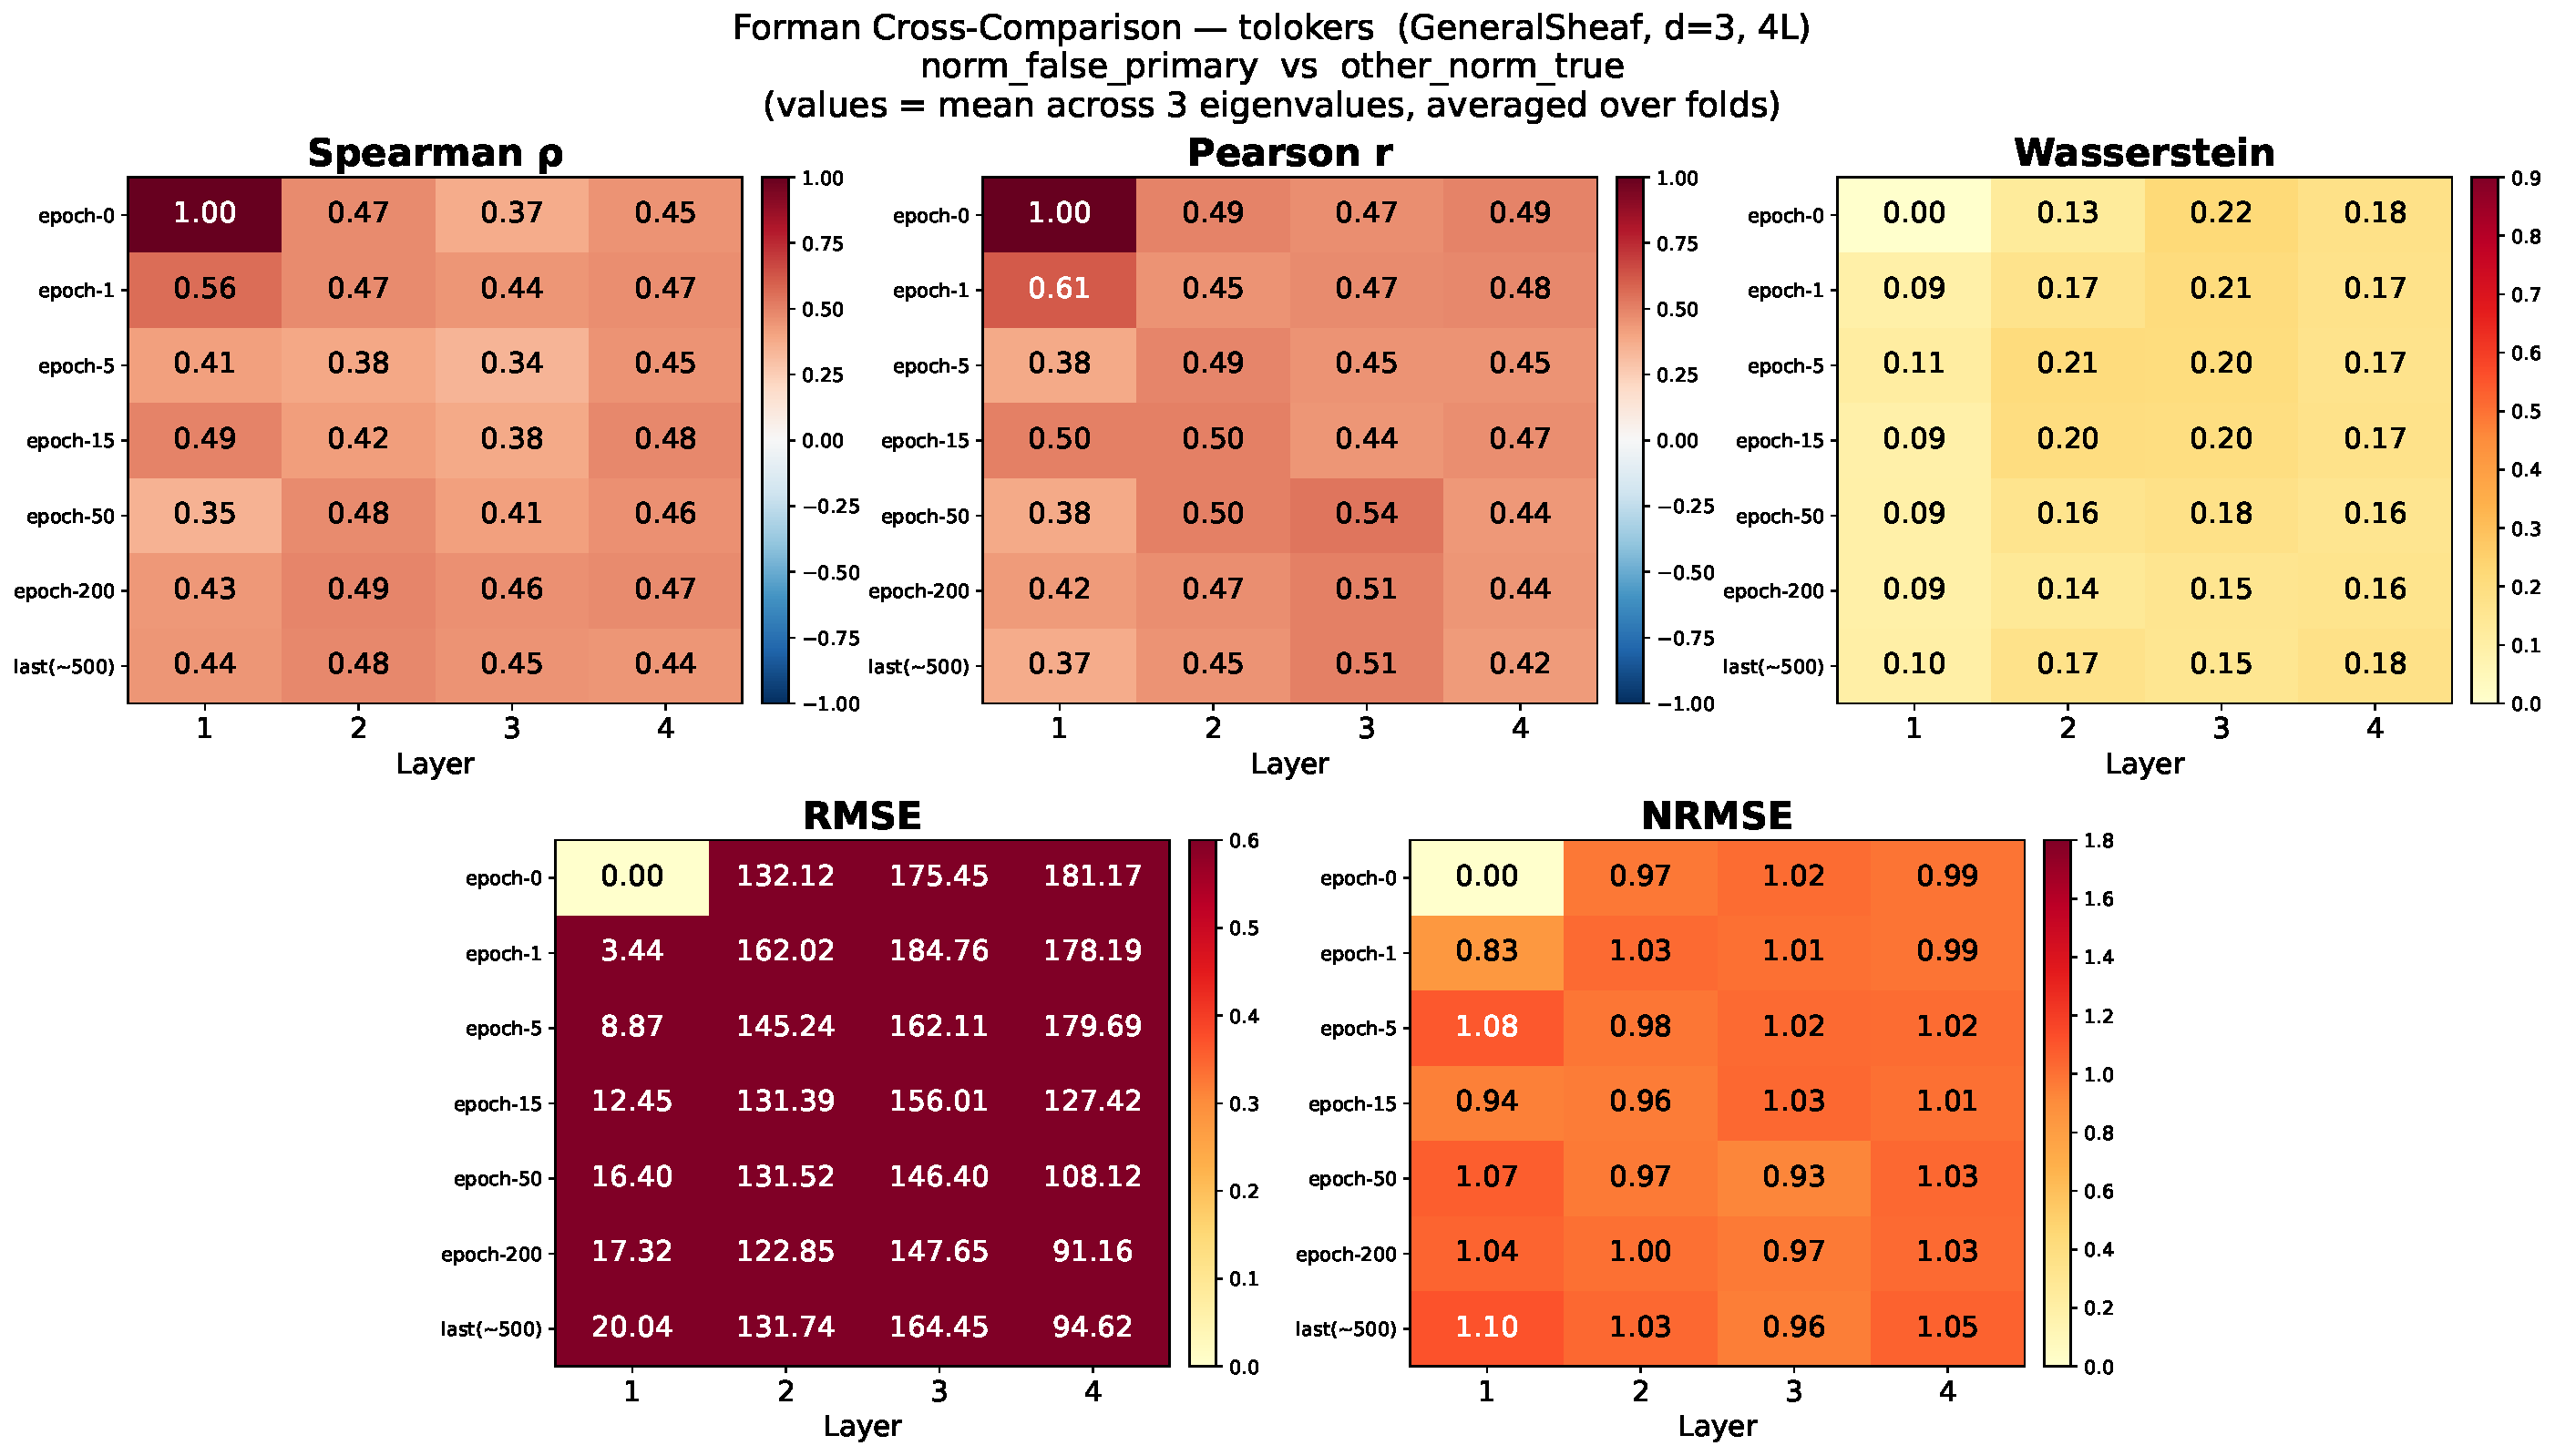
\includegraphics[width=\linewidth]{heatmaps/comparison/norm_false_vs_other_norm_true/tolokers_GeneralSheaf_d3_4L_norm_false_primary_vs_other_norm_true_heatmap.pdf}
\end{figure}
\end{frame}

\begin{frame}{Wisconsin --- Dir B: maps norm=False vs maps norm=True (both unnorm. $\Delta_{\mathcal{F}}$)}
\begin{figure}
    \centering
    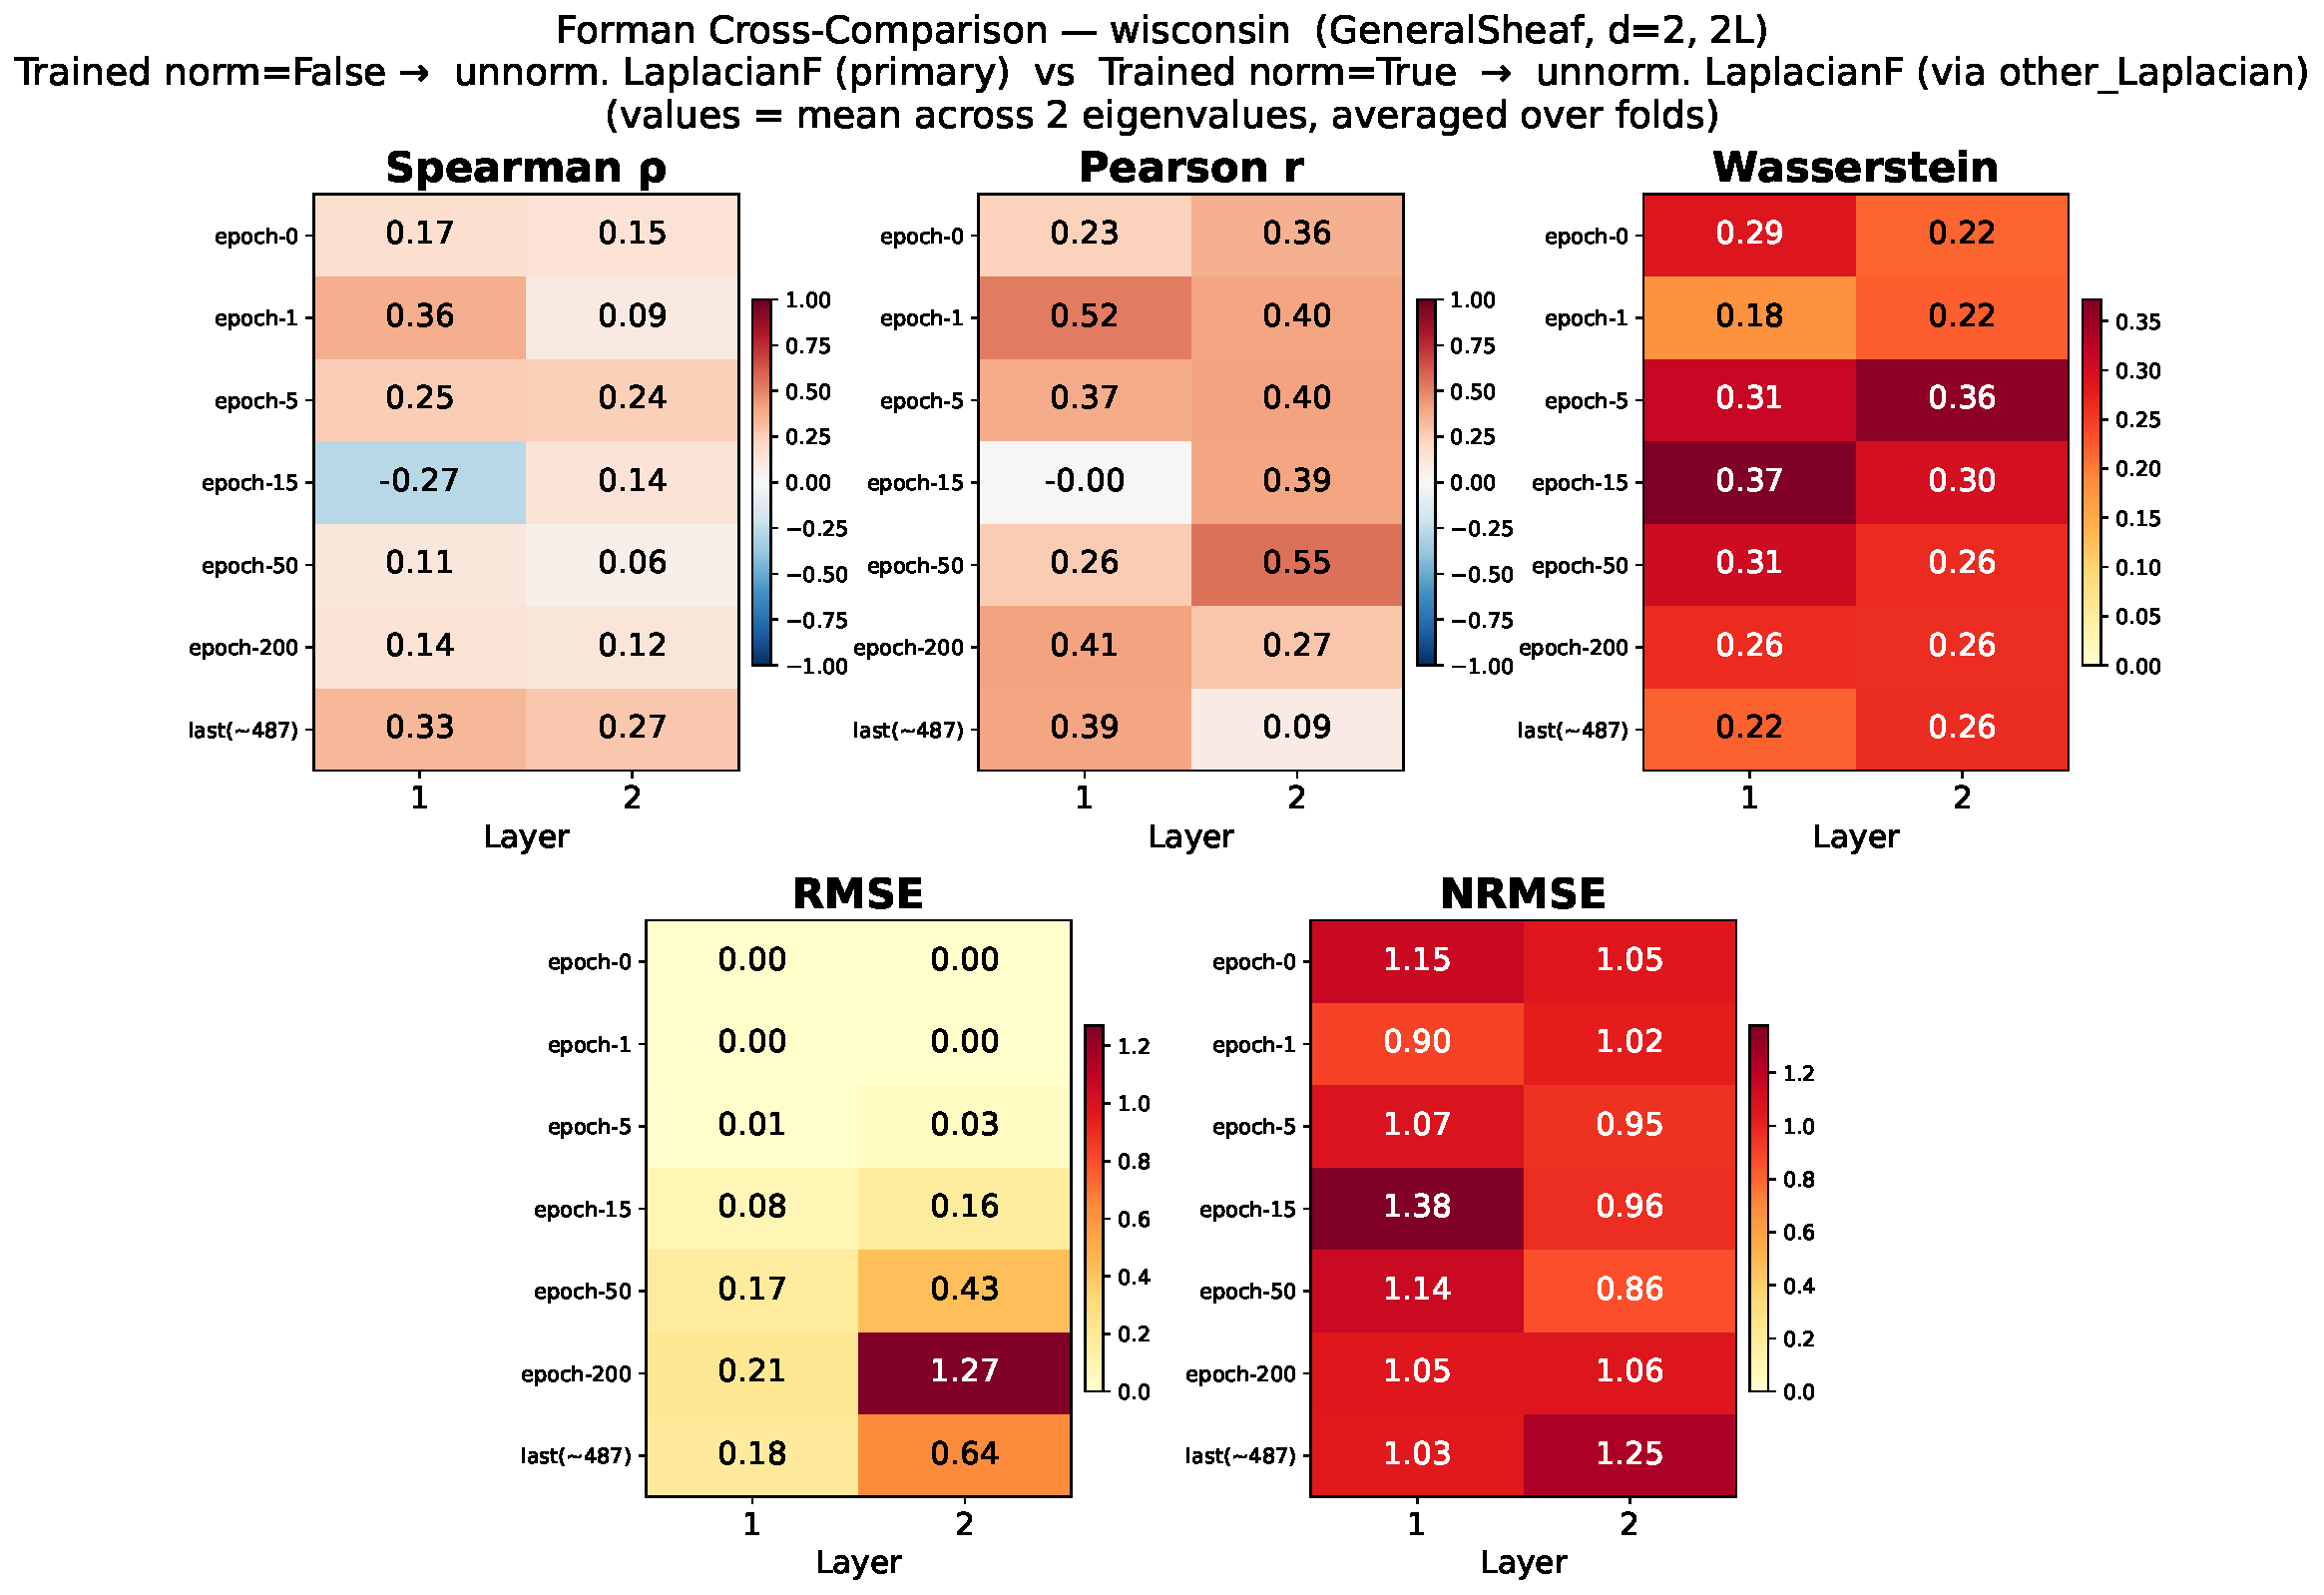
\includegraphics[width=\linewidth]{heatmaps/comparison/norm_false_vs_other_norm_true/wisconsin_GeneralSheaf_d2_2L_norm_false_primary_vs_other_norm_true_heatmap.pdf}
\end{figure}
\end{frame}

% ══════════════════════════════════════════════════════════════════════════════
%  SECTION 5 — JointSheafParams, normalised=False, identity maps
% ══════════════════════════════════════════════════════════════════════════════

\begin{frame}{}
\centering
\Huge\textbf{JointSheafParams}\\[6pt]
\Large Norm=False, Identity Initial Maps
\end{frame}

\begin{frame}{Amazon Ratings --- Joint, $d=5$, $L=5$, Norm=False, Identity}
\begin{figure}
    \centering
    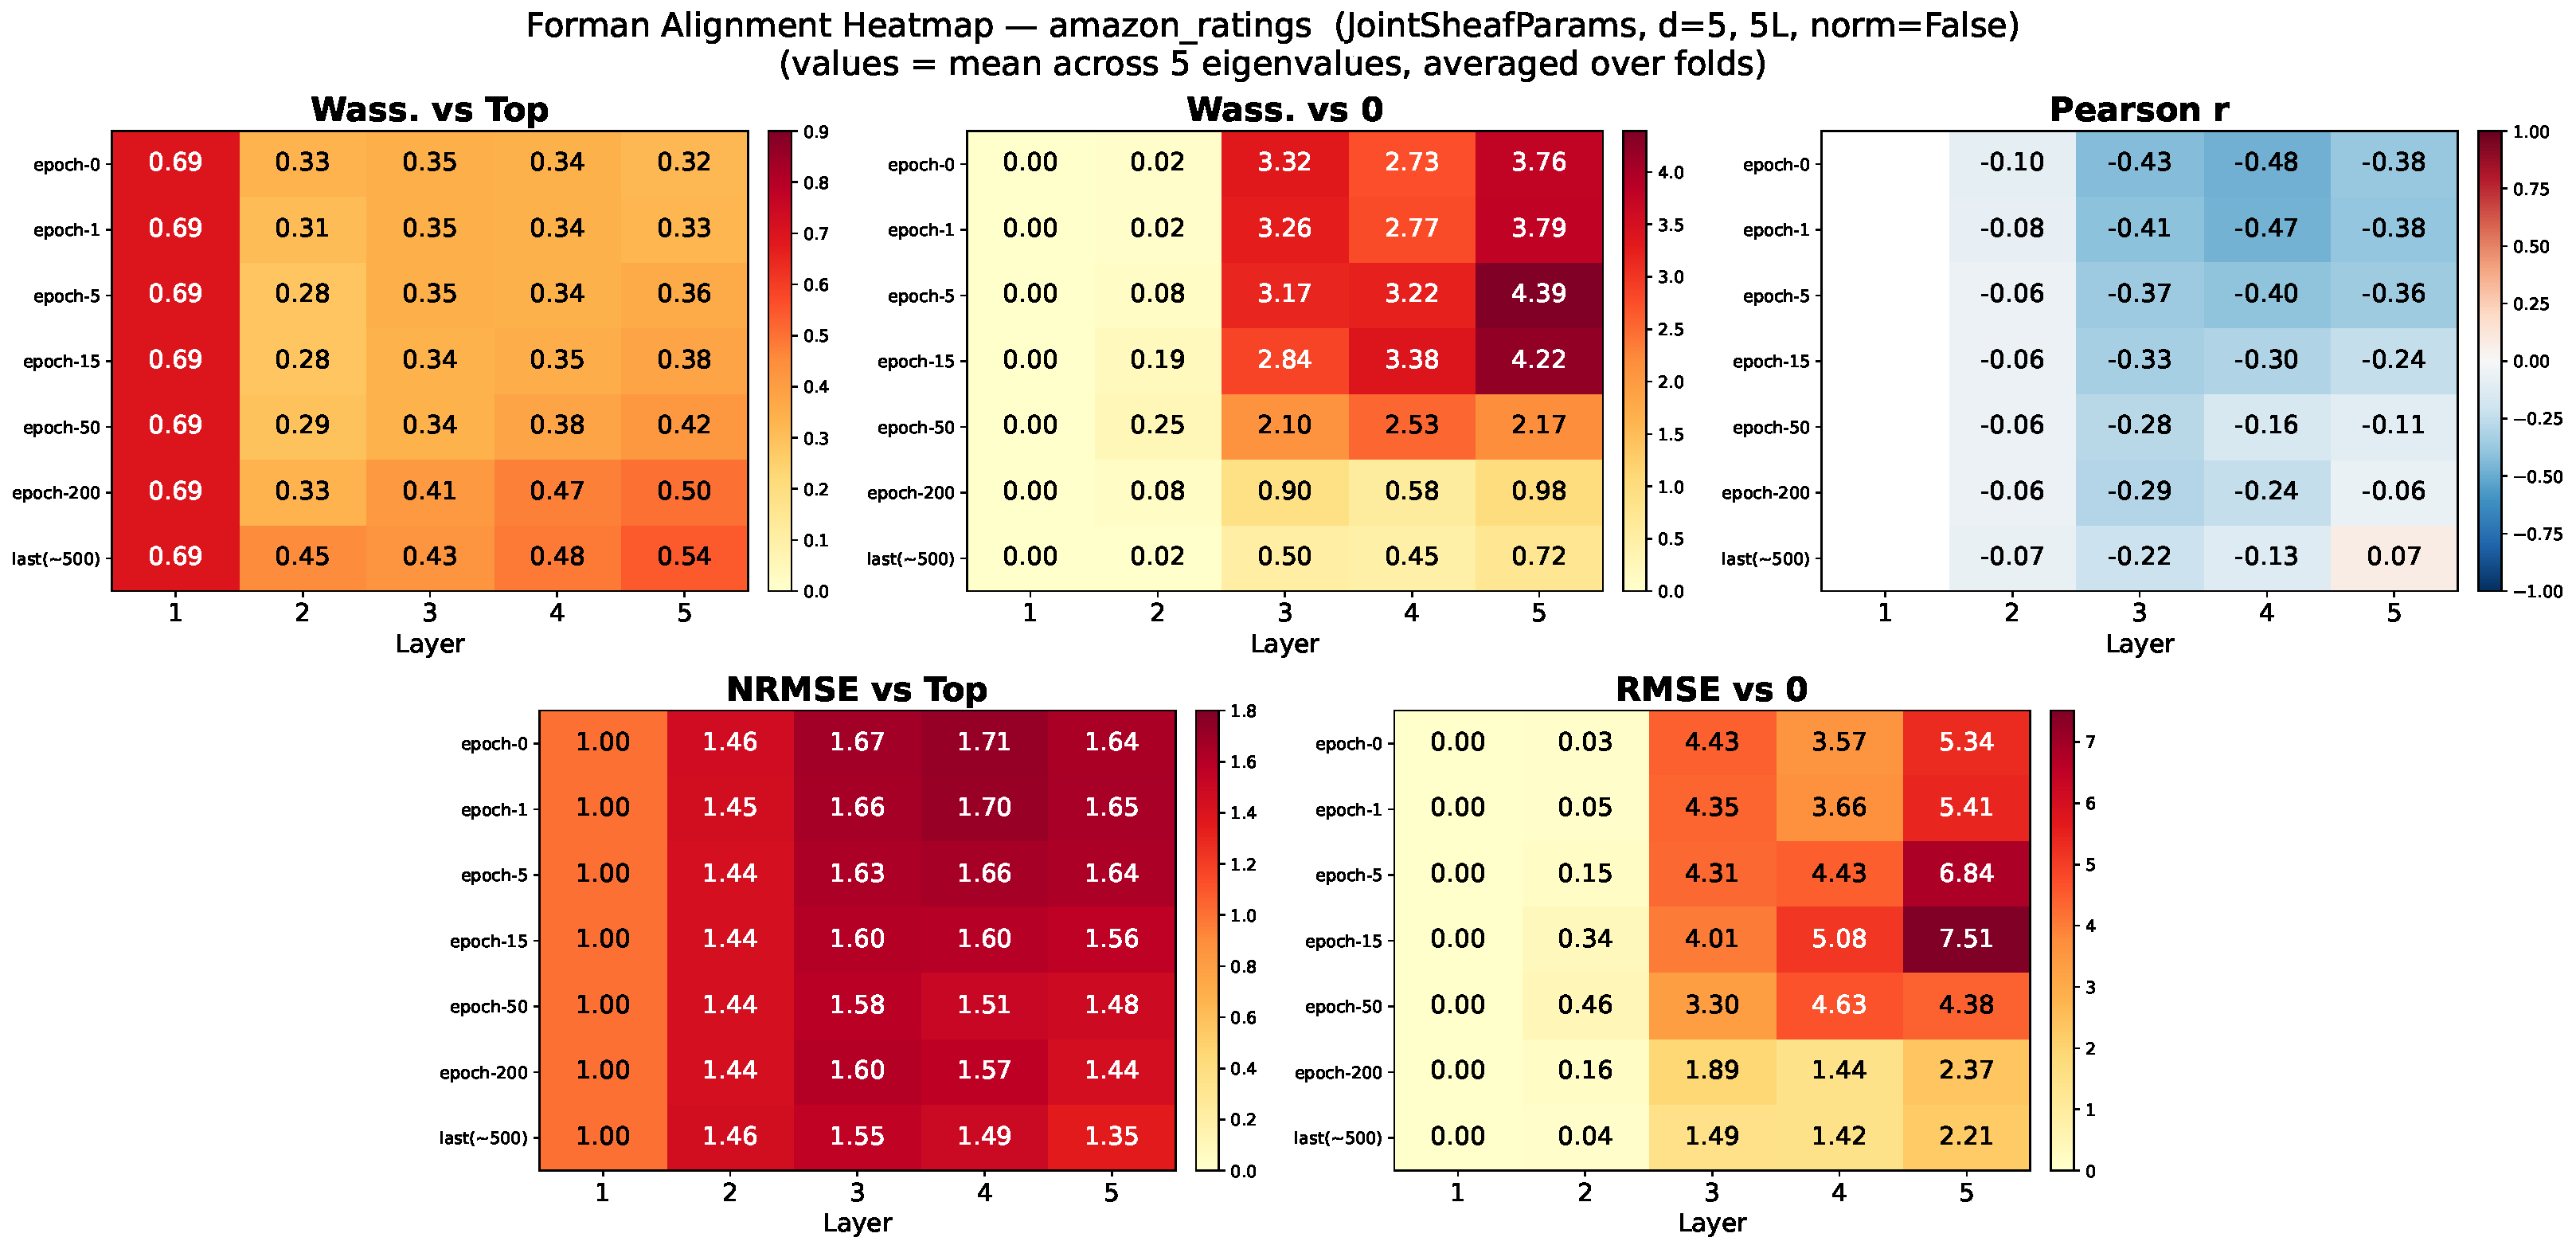
\includegraphics[width=\linewidth]{heatmaps/JointSheafParams/normalised_false/first_maps_identity/amazon_ratings_JointSheafParams_d5_5L_Norm_False_first_maps_identity_heatmap.pdf}
\end{figure}
\end{frame}

\begin{frame}{Citeseer --- Joint, $d=5$, $L=4$, Norm=False, Identity}
\begin{figure}
    \centering
    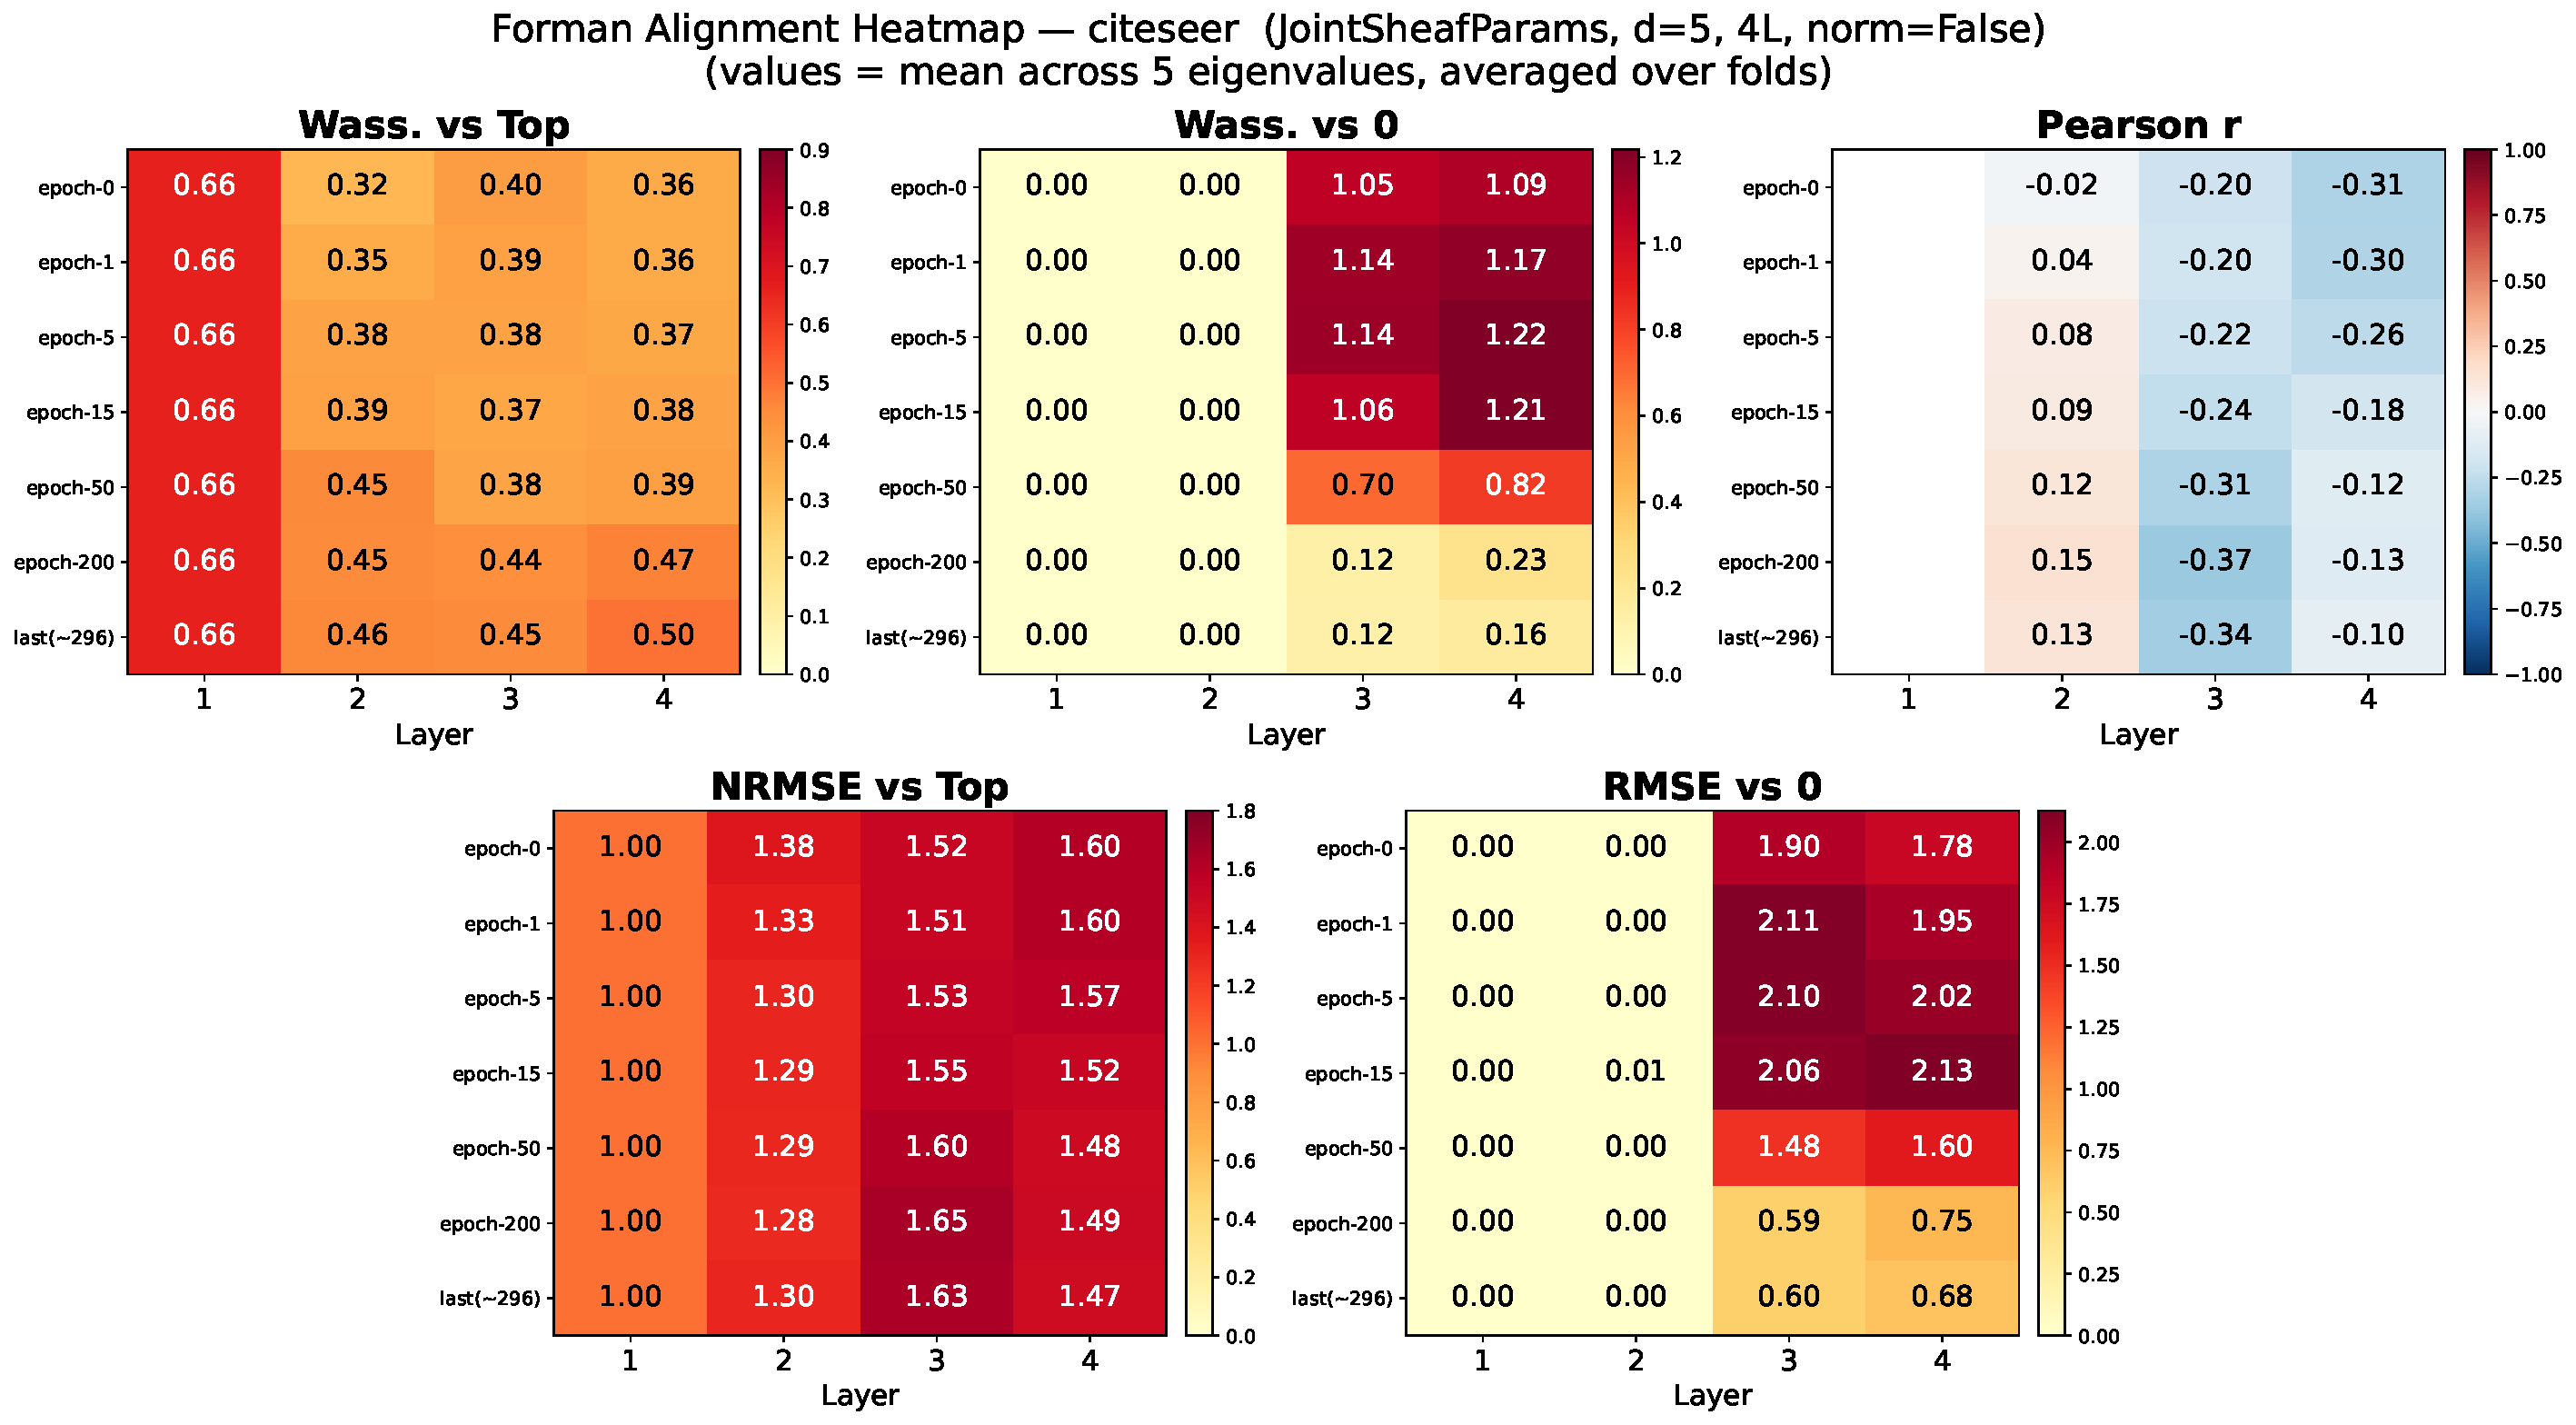
\includegraphics[width=\linewidth]{heatmaps/JointSheafParams/normalised_false/first_maps_identity/citeseer_JointSheafParams_d5_4L_Norm_False_first_maps_identity_heatmap.pdf}
\end{figure}
\end{frame}

\begin{frame}{Cora --- Joint, $d=3$, $L=3$, Norm=False, Identity}
\begin{figure}
    \centering
    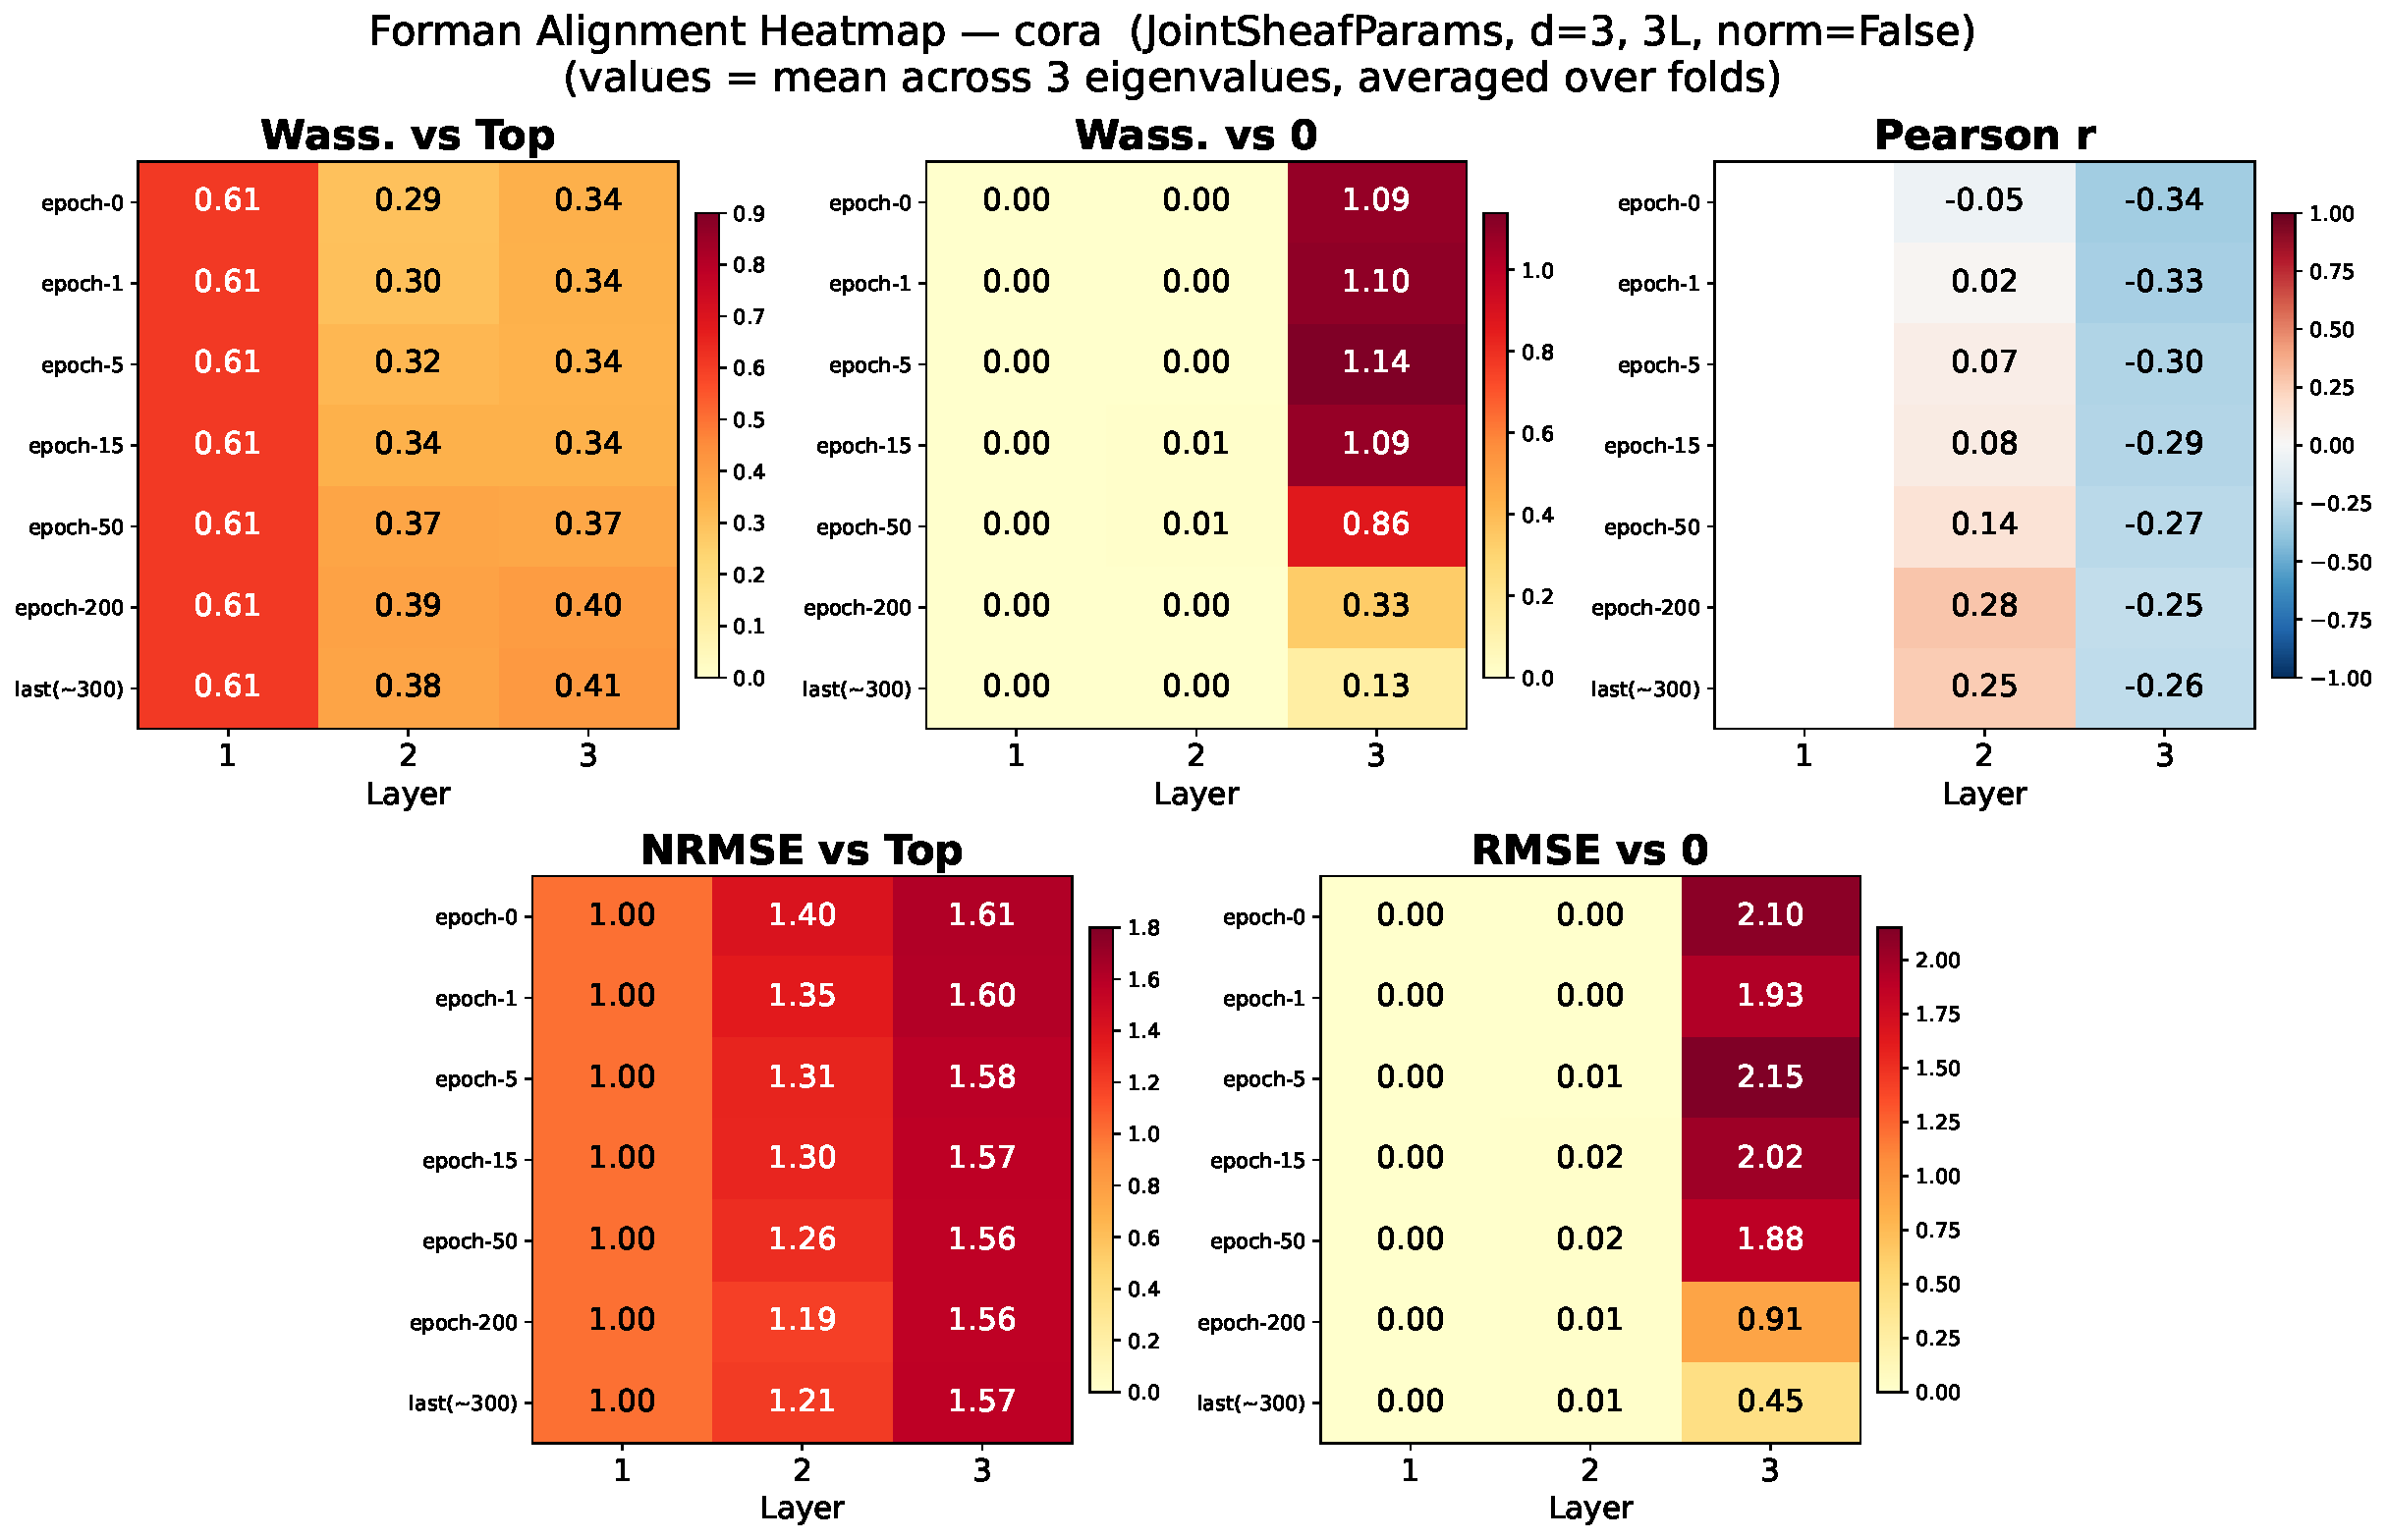
\includegraphics[width=\linewidth]{heatmaps/JointSheafParams/normalised_false/first_maps_identity/cora_JointSheafParams_d3_3L_Norm_False_first_maps_identity_heatmap.pdf}
\end{figure}
\end{frame}

\begin{frame}{Cornell --- Joint, $d=2$, $L=2$, Norm=False, Identity}
\begin{figure}
    \centering
    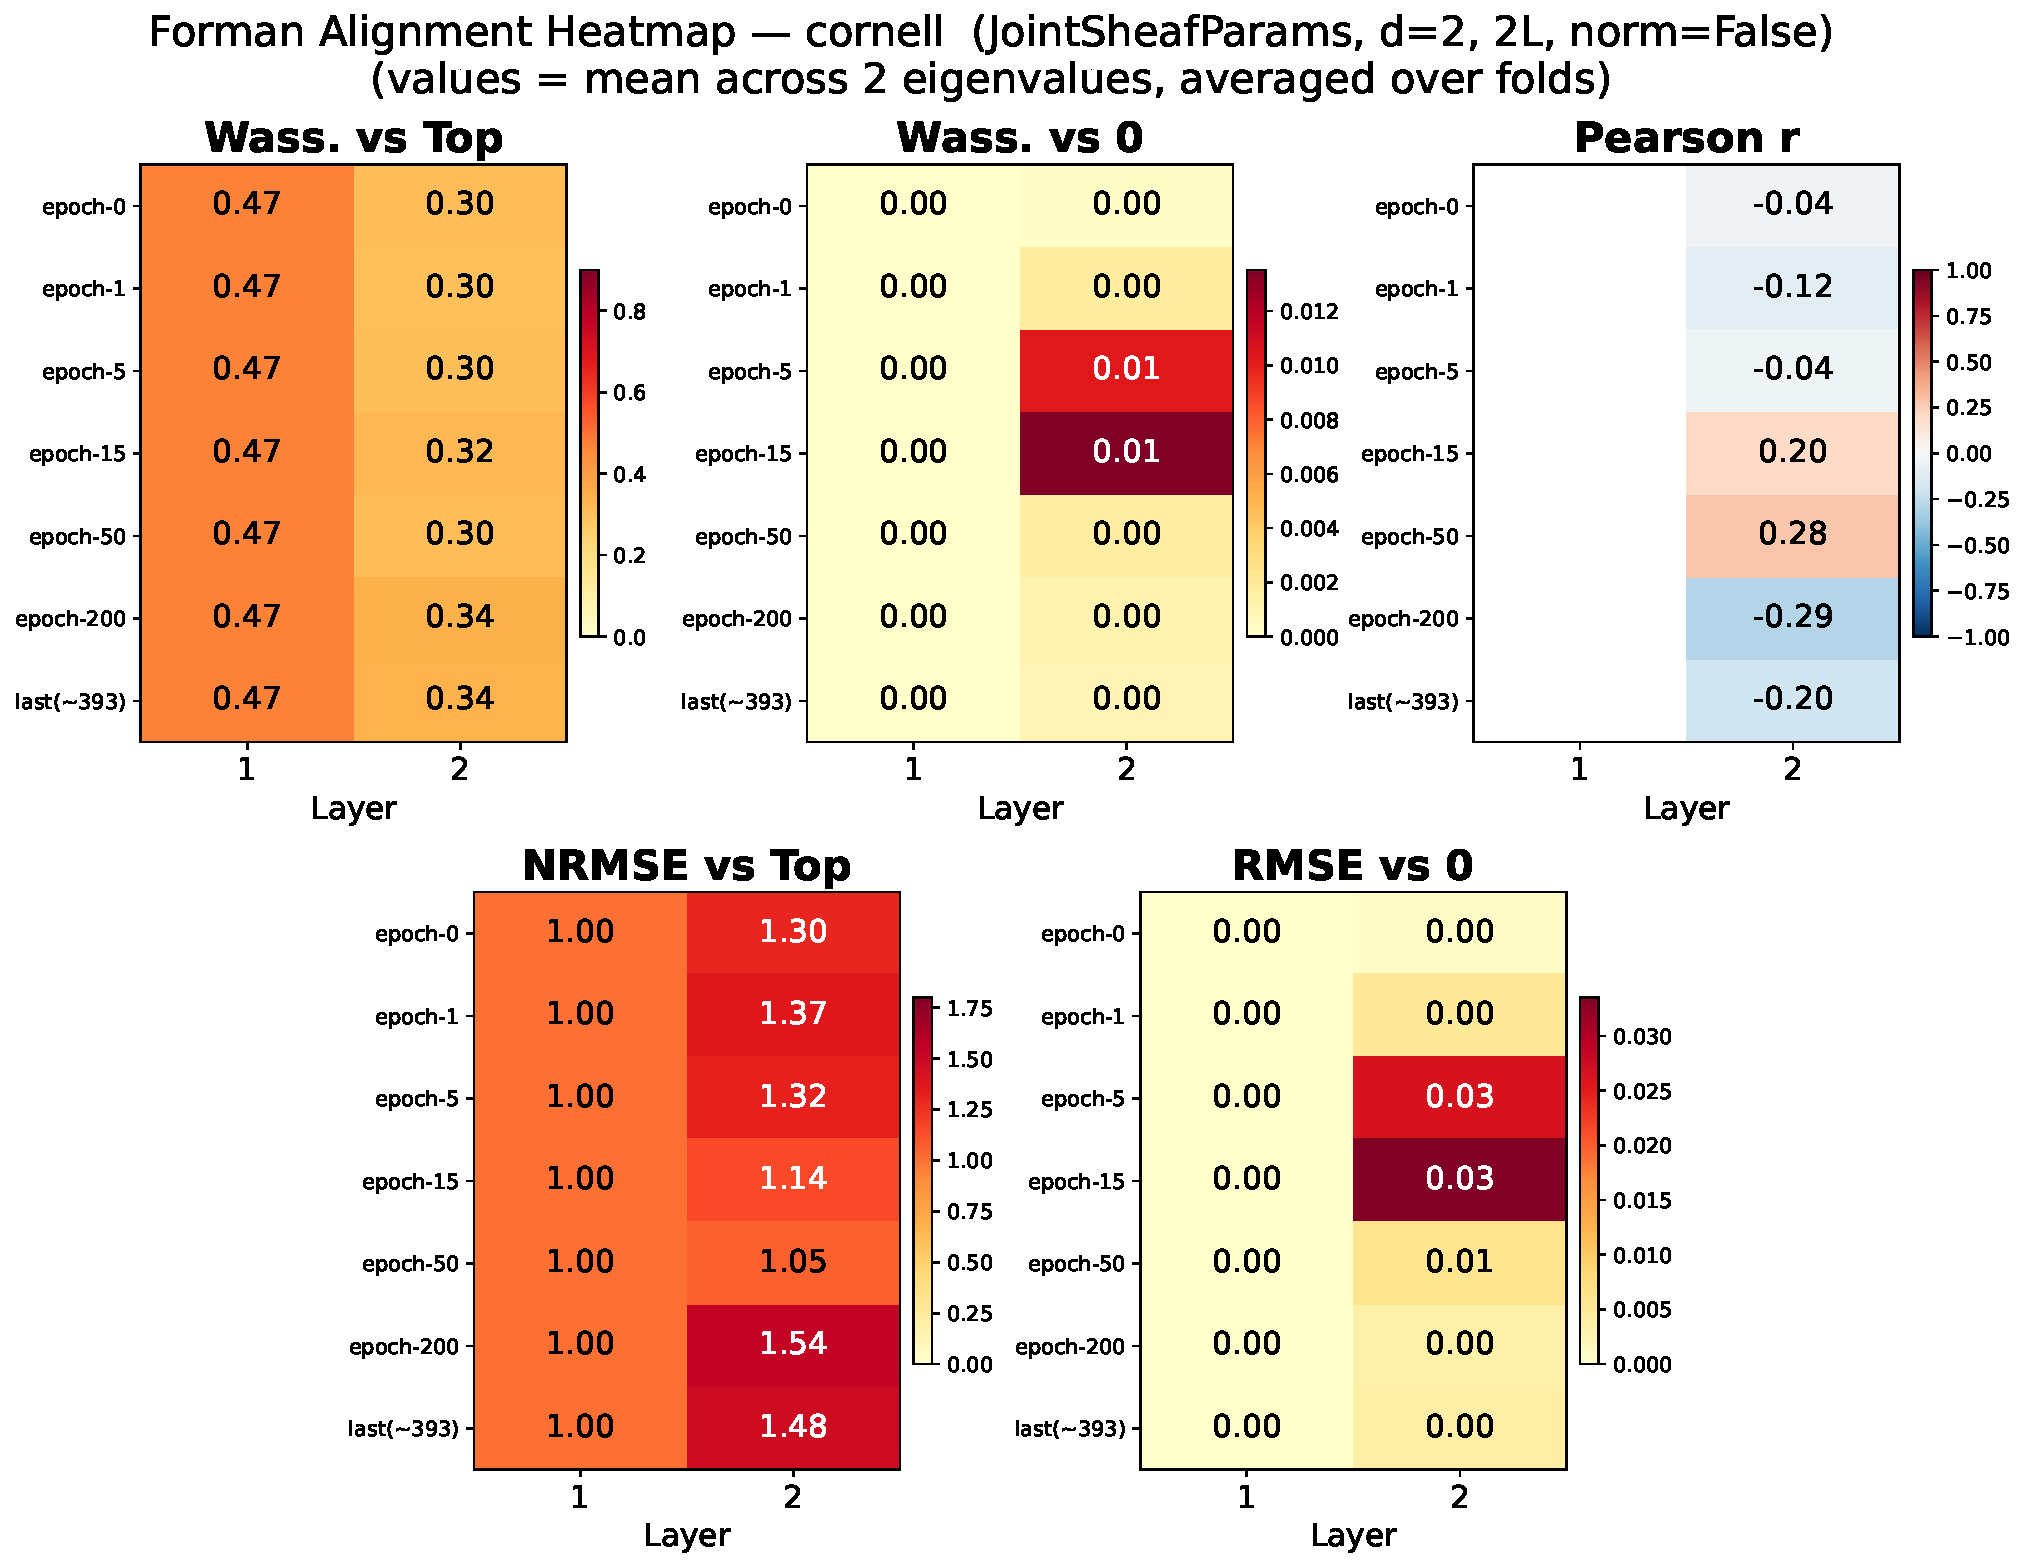
\includegraphics[width=\linewidth]{heatmaps/JointSheafParams/normalised_false/first_maps_identity/cornell_JointSheafParams_d2_2L_Norm_False_first_maps_identity_heatmap.pdf}
\end{figure}
\end{frame}

\begin{frame}{Minesweeper --- Joint, $d=5$, $L=6$, Norm=False, Identity}
\begin{figure}
    \centering
    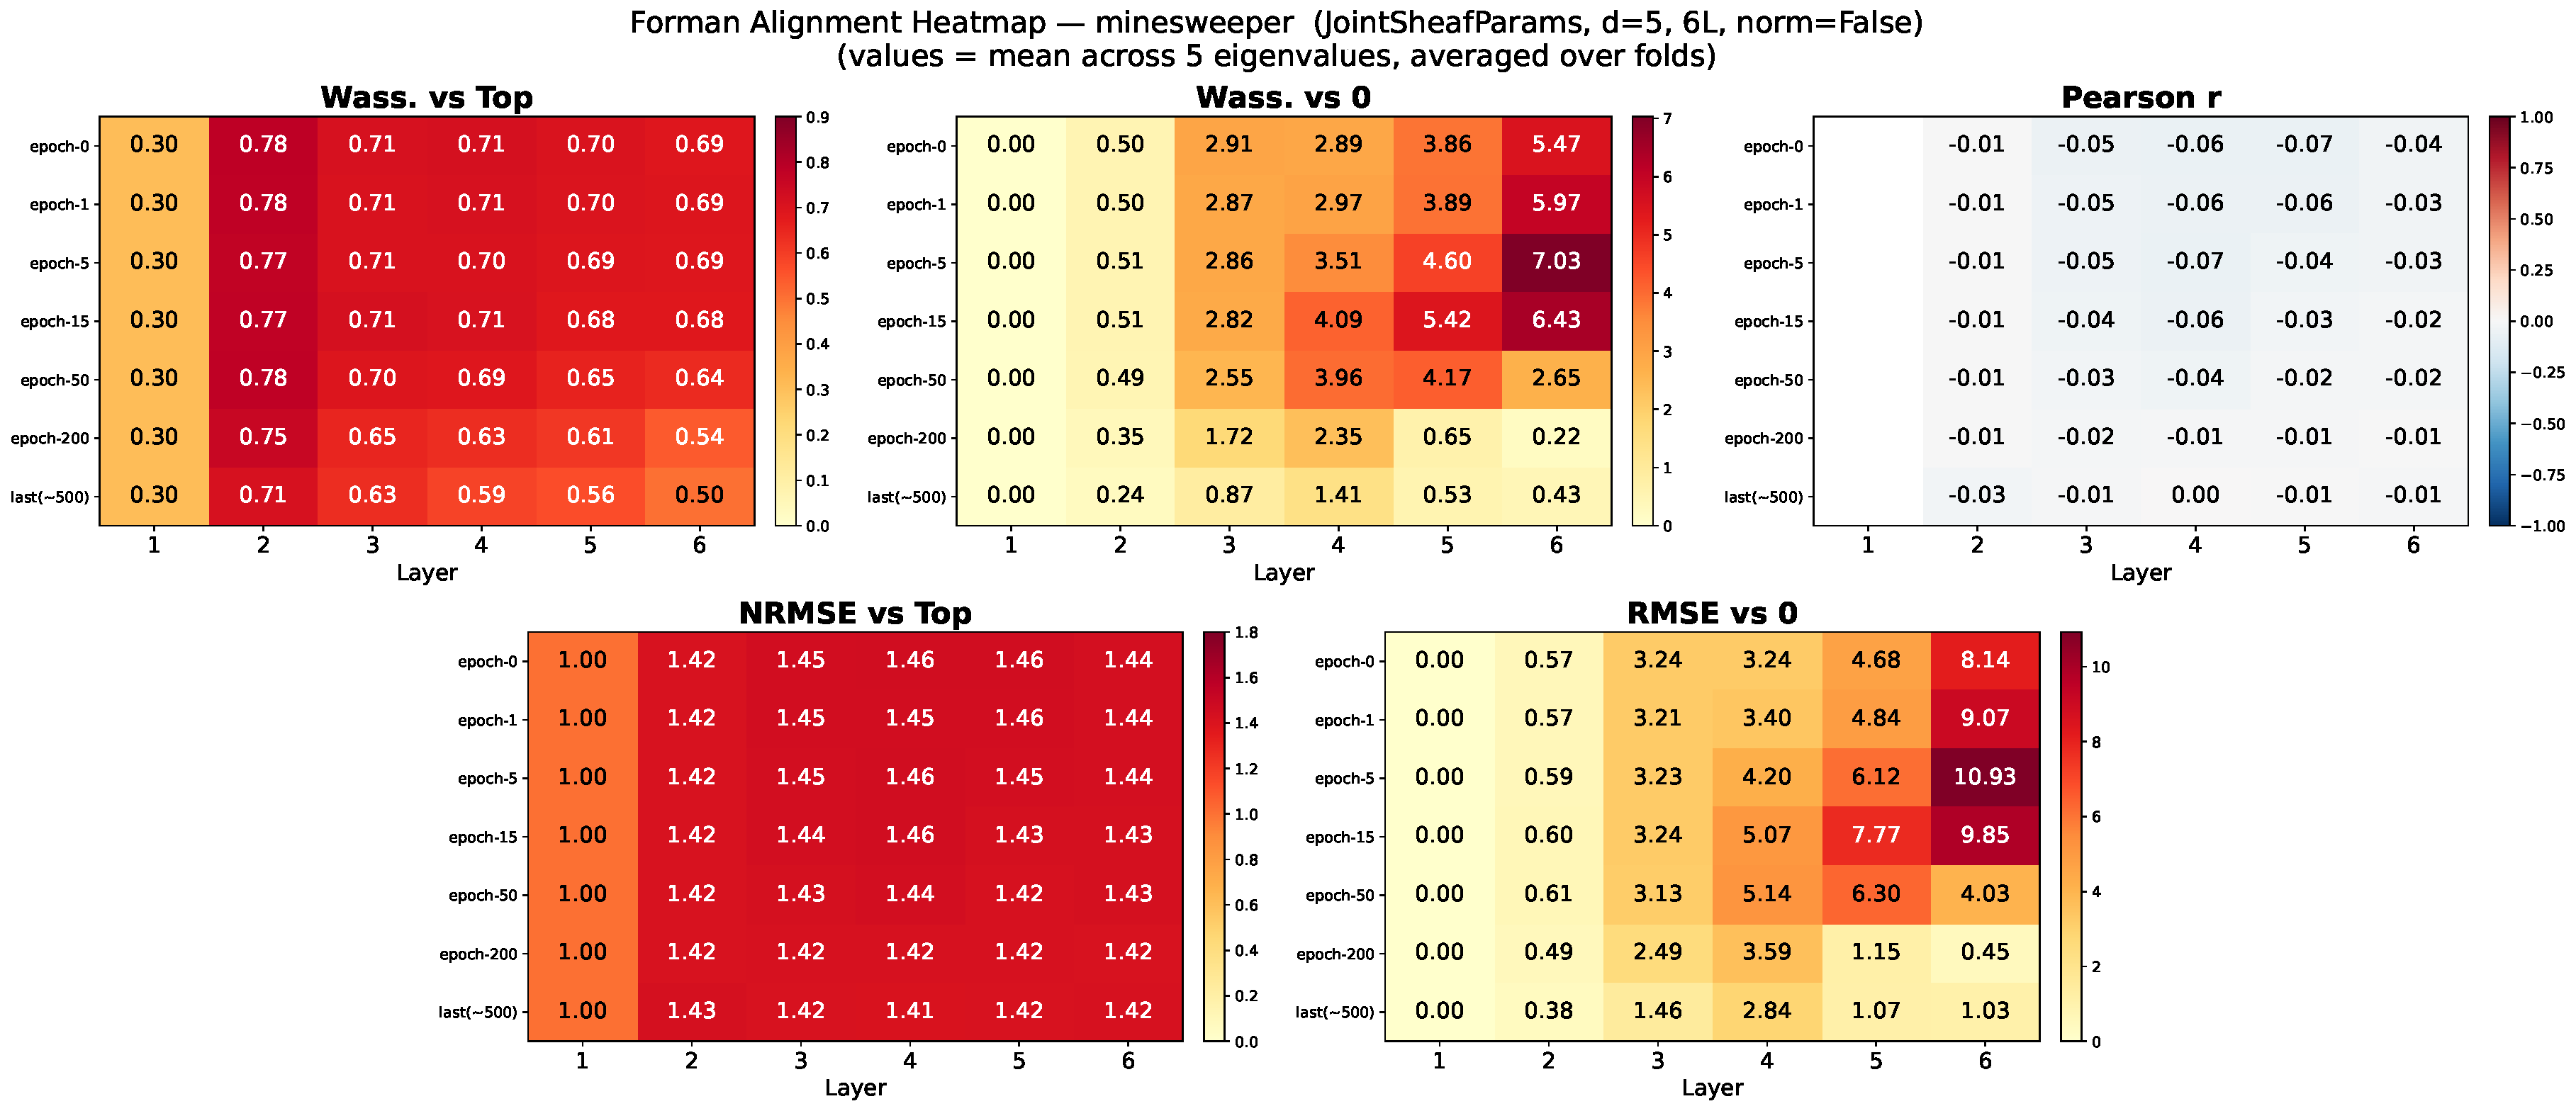
\includegraphics[width=\linewidth]{heatmaps/JointSheafParams/normalised_false/first_maps_identity/minesweeper_JointSheafParams_d5_6L_Norm_False_first_maps_identity_heatmap.pdf}
\end{figure}
\end{frame}

\begin{frame}{Pubmed --- Joint, $d=5$, $L=4$, Norm=False, Identity}
\begin{figure}
    \centering
    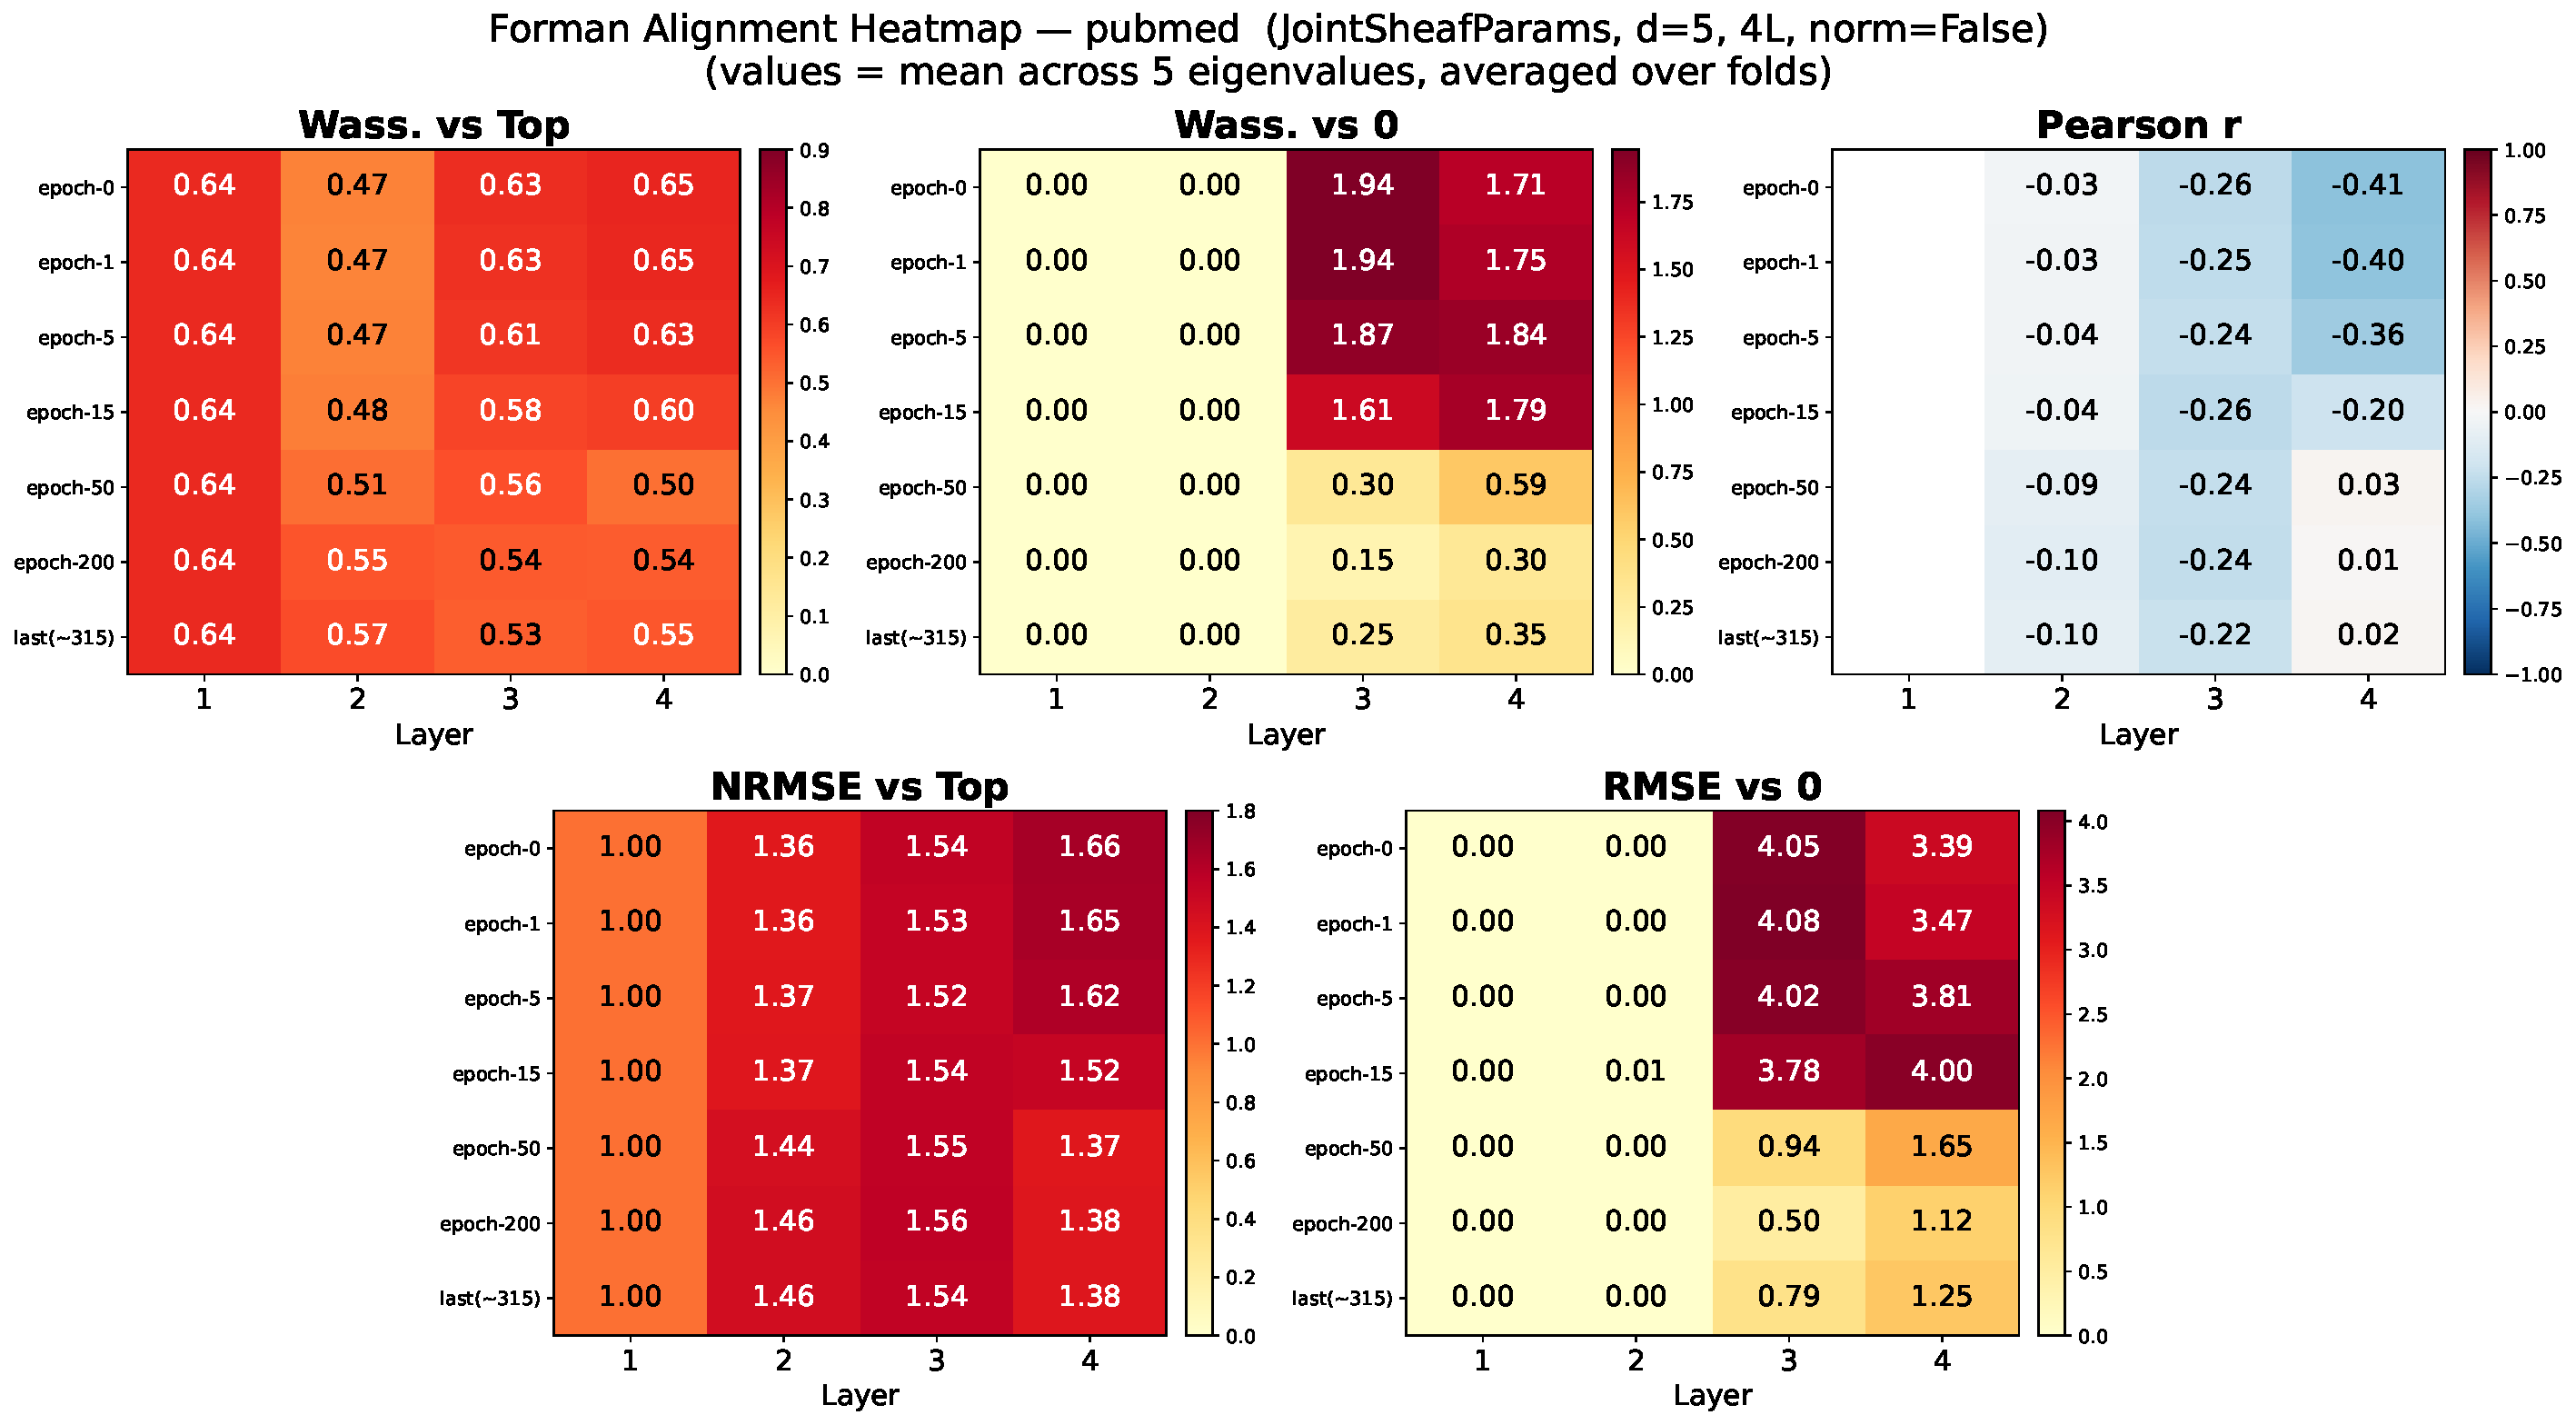
\includegraphics[width=\linewidth]{heatmaps/JointSheafParams/normalised_false/first_maps_identity/pubmed_JointSheafParams_d5_4L_Norm_False_first_maps_identity_heatmap.pdf}
\end{figure}
\end{frame}

\begin{frame}{Questions --- Joint, $d=5$, $L=4$, Norm=False, Identity}
\begin{figure}
    \centering
    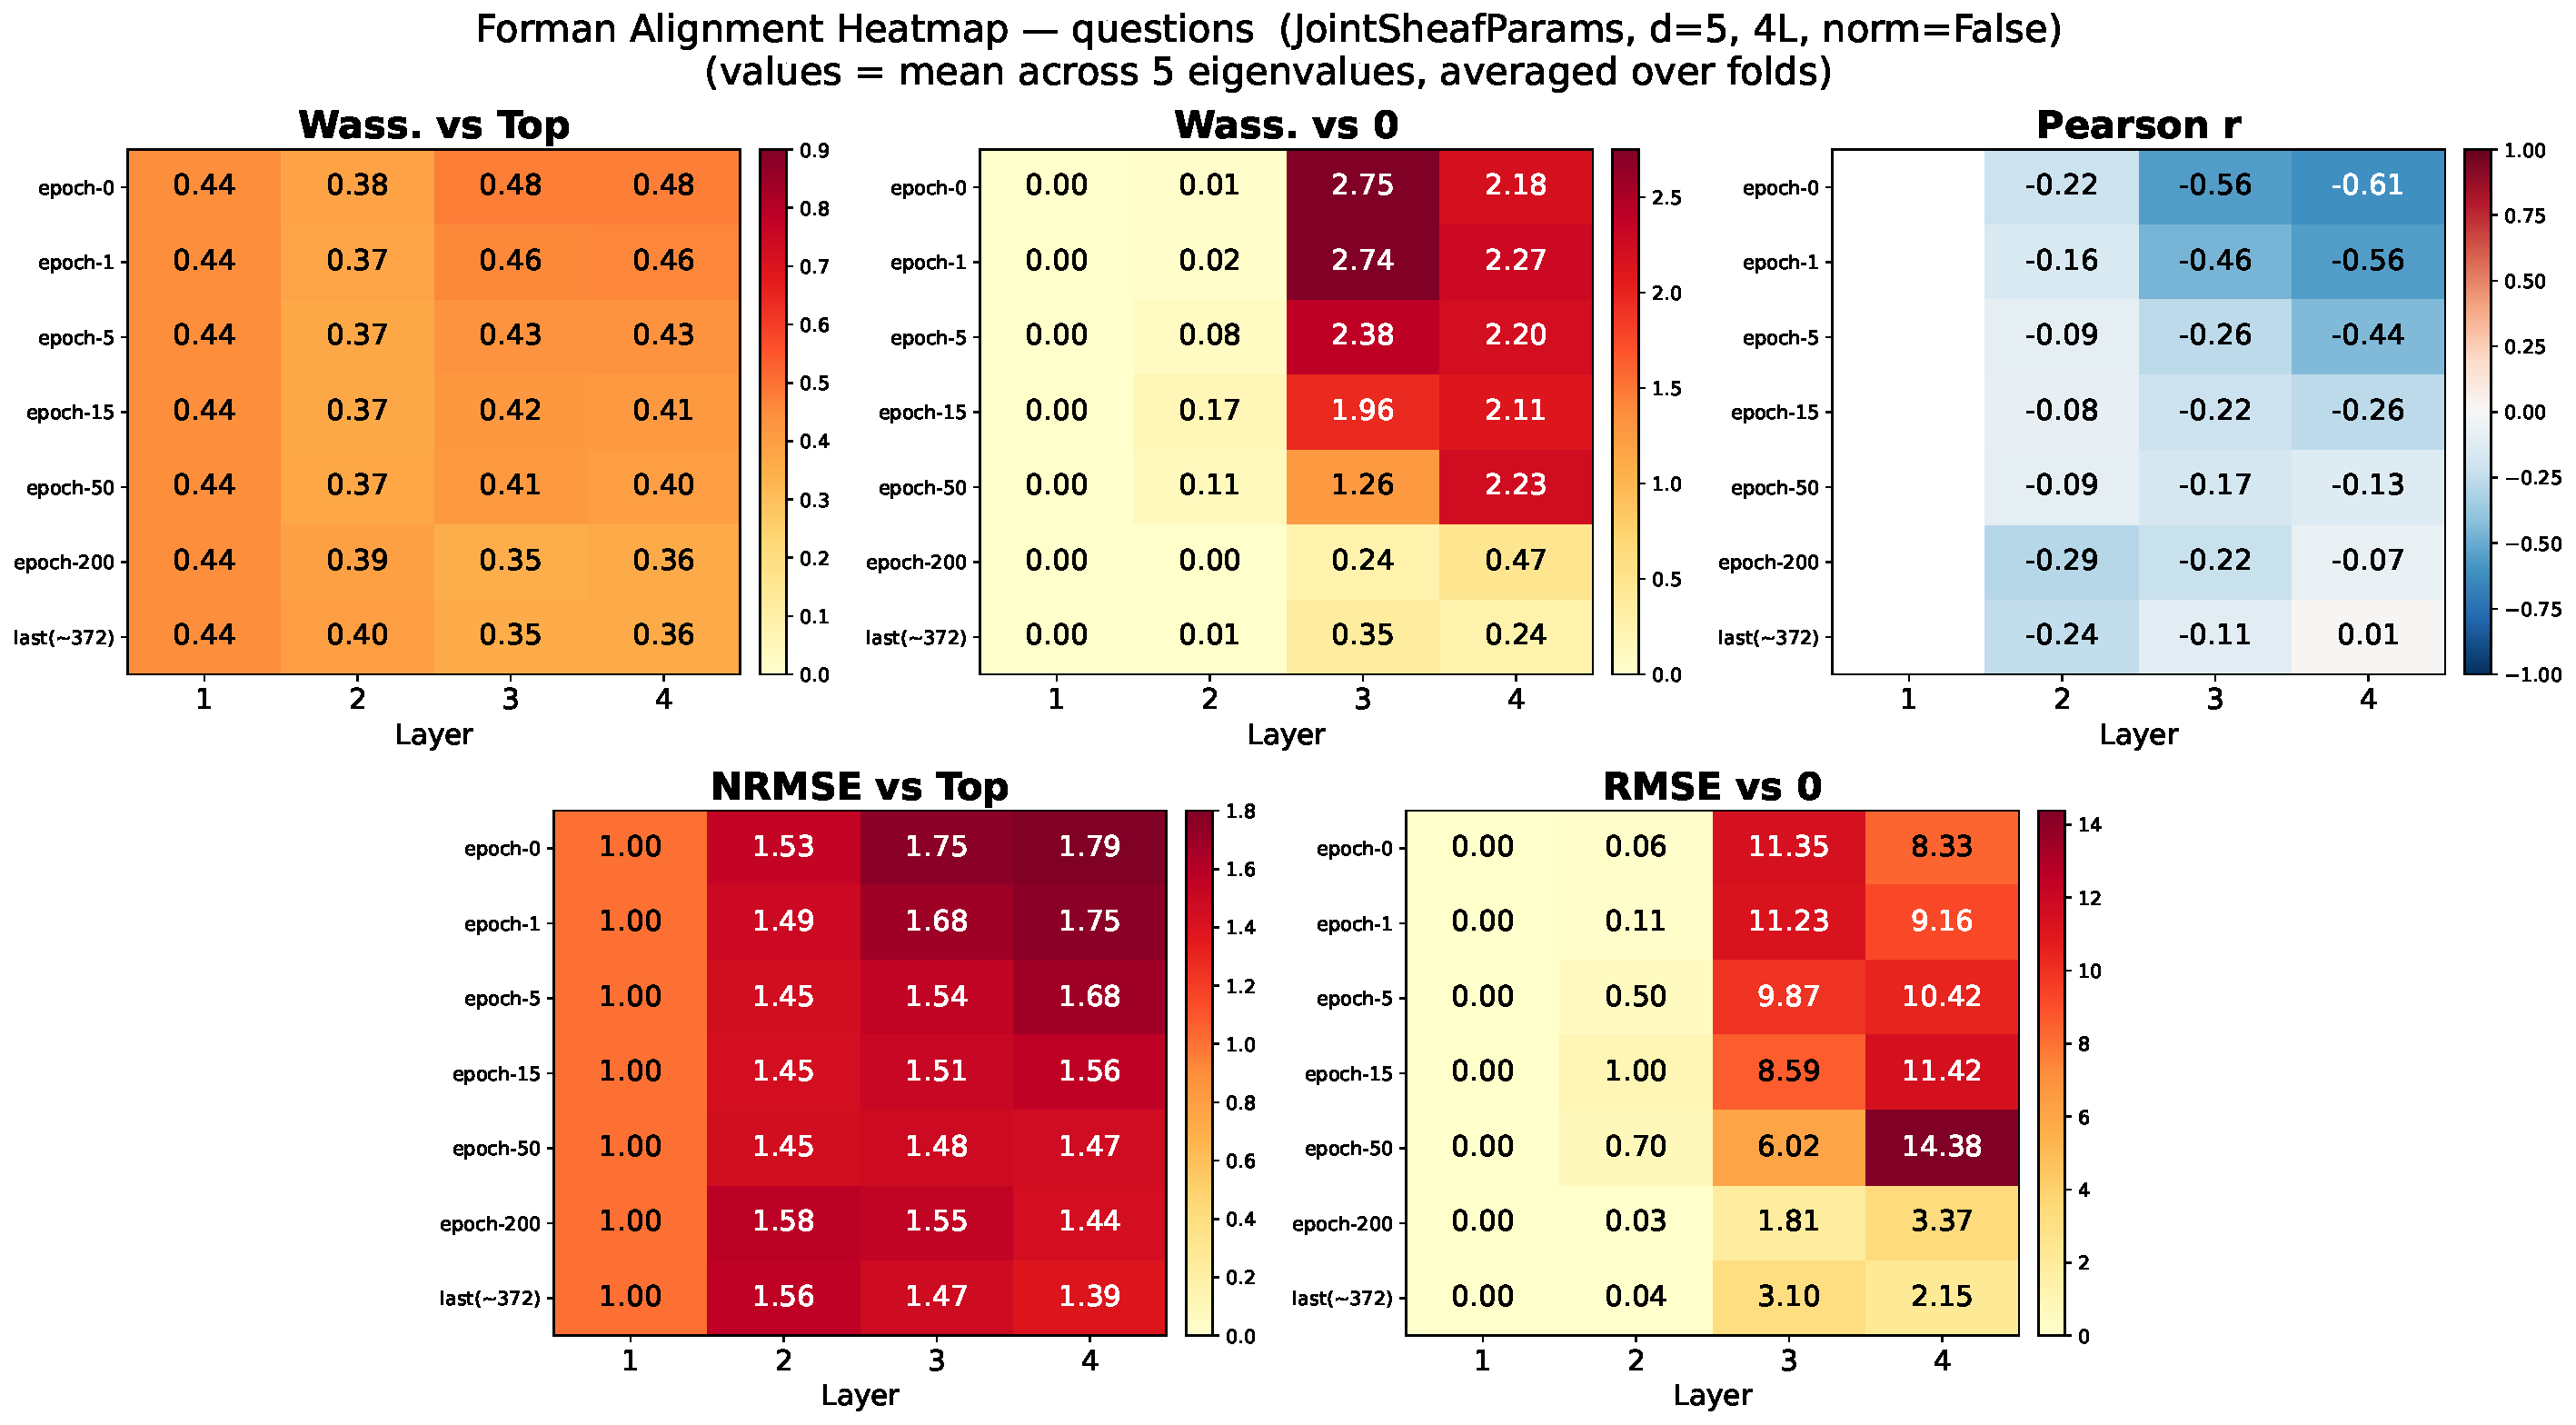
\includegraphics[width=\linewidth]{heatmaps/JointSheafParams/normalised_false/first_maps_identity/questions_JointSheafParams_d5_4L_Norm_False_first_maps_identity_heatmap.pdf}
\end{figure}
\end{frame}

\begin{frame}{Roman Empire --- Joint, $d=5$, $L=5$, Norm=False, Identity}
\begin{figure}
    \centering
    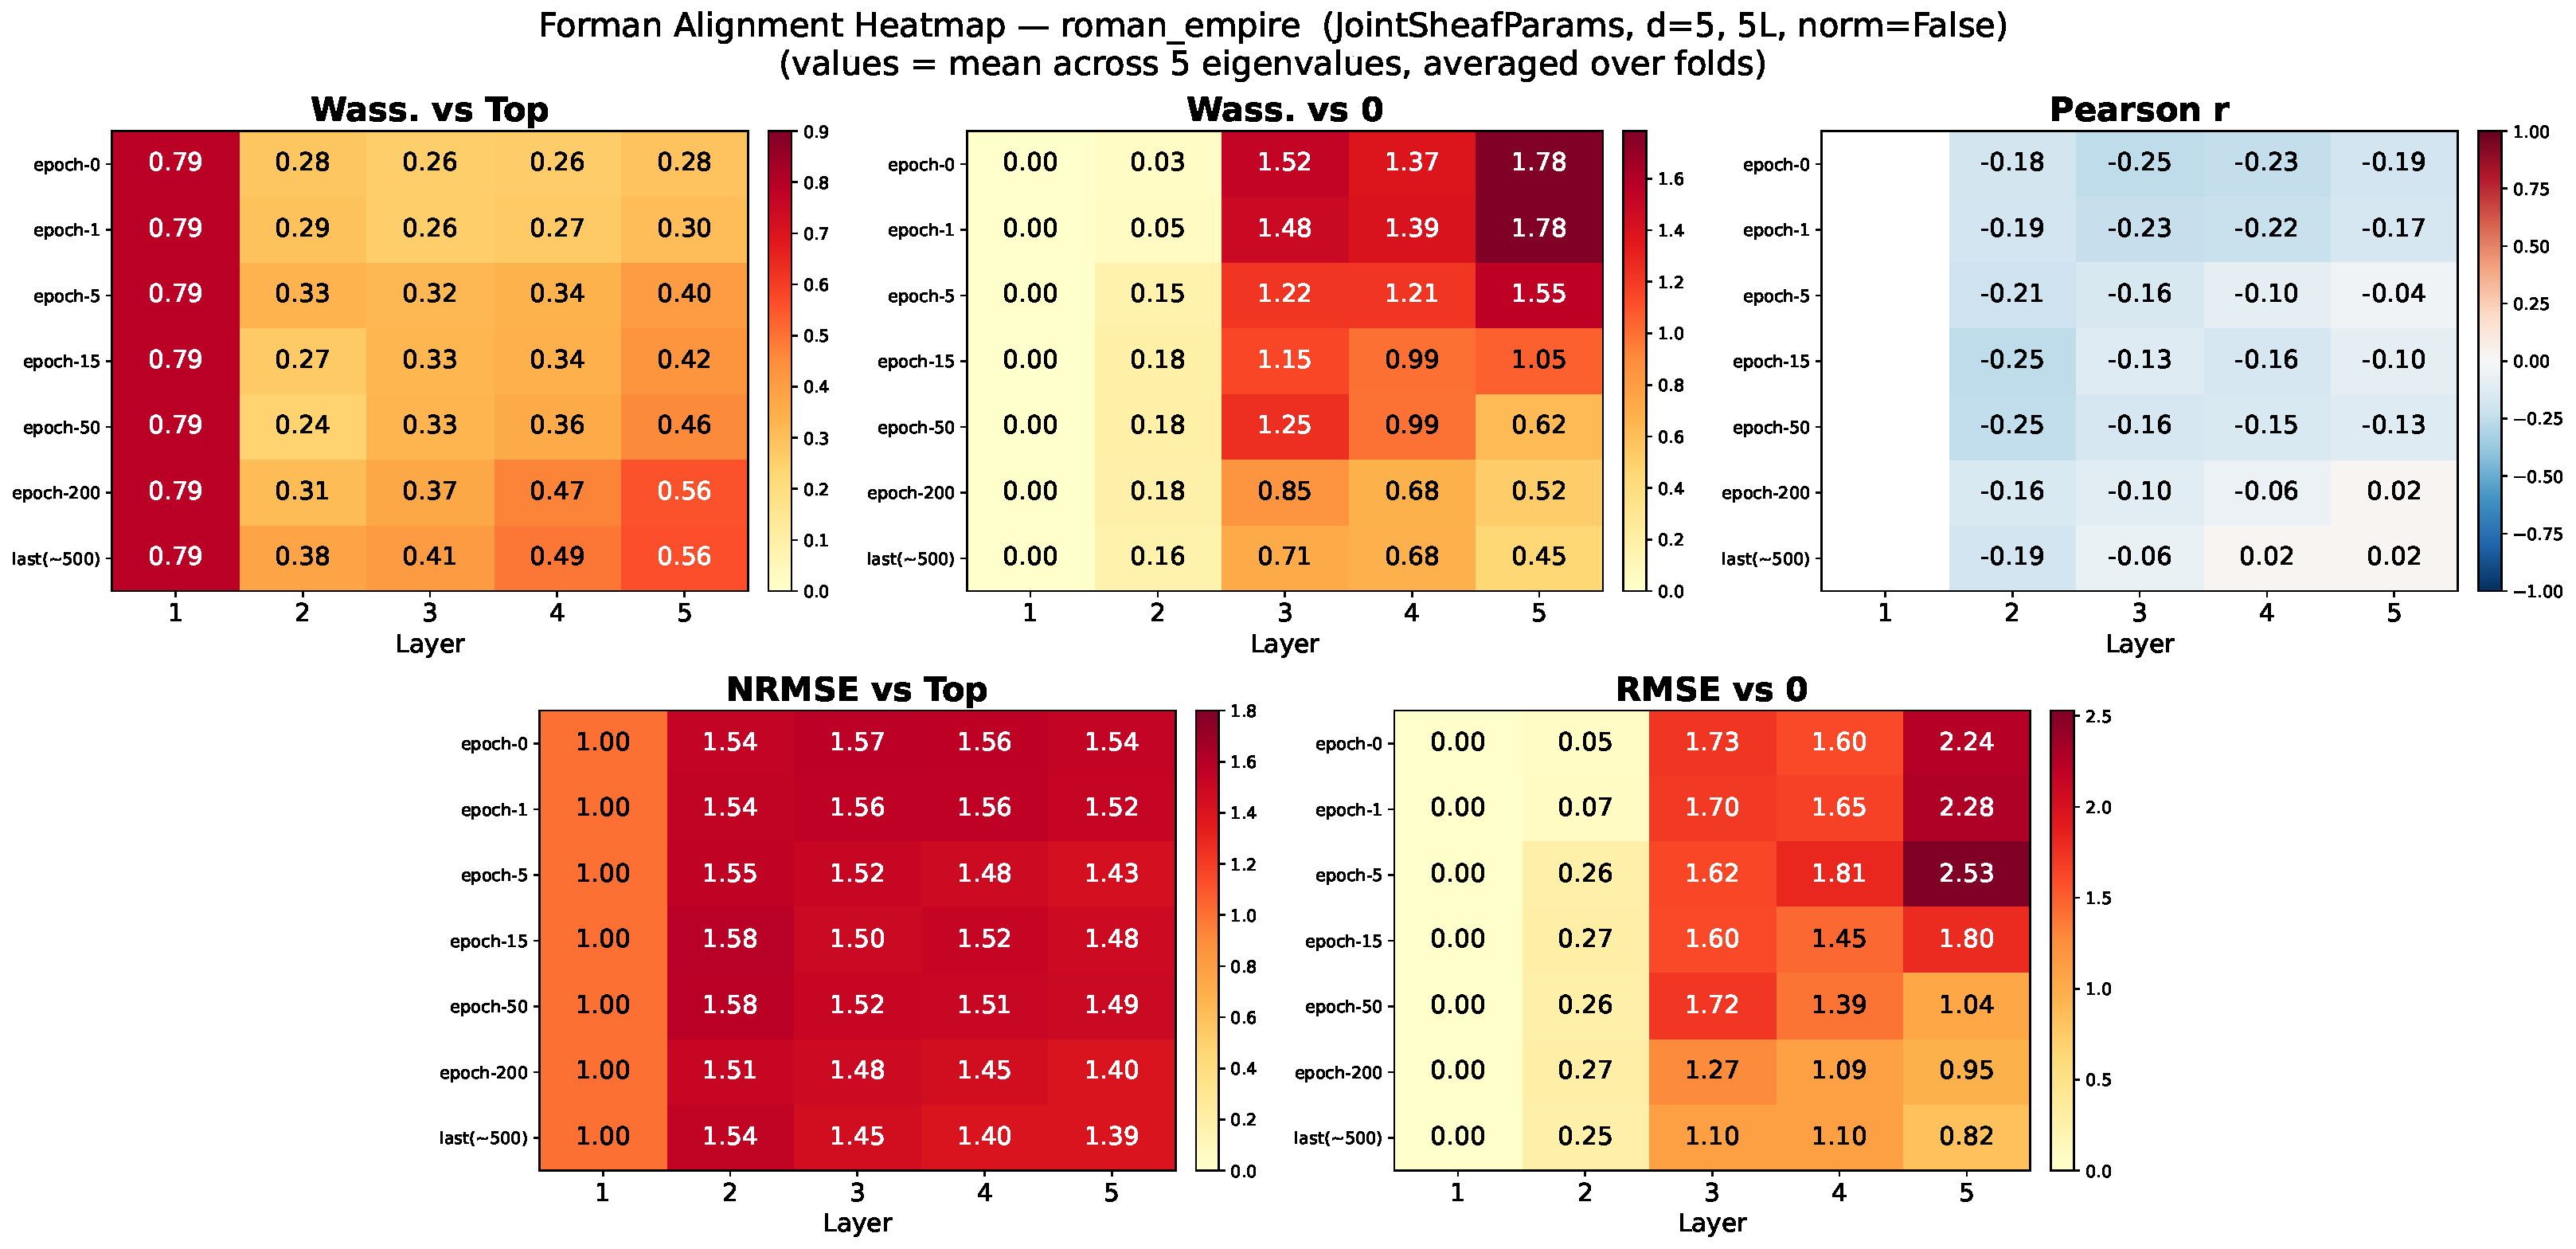
\includegraphics[width=\linewidth]{heatmaps/JointSheafParams/normalised_false/first_maps_identity/roman_empire_JointSheafParams_d5_5L_Norm_False_first_maps_identity_heatmap.pdf}
\end{figure}
\end{frame}

\begin{frame}{Tolokers --- Joint, $d=3$, $L=4$, Norm=False, Identity}
\begin{figure}
    \centering
    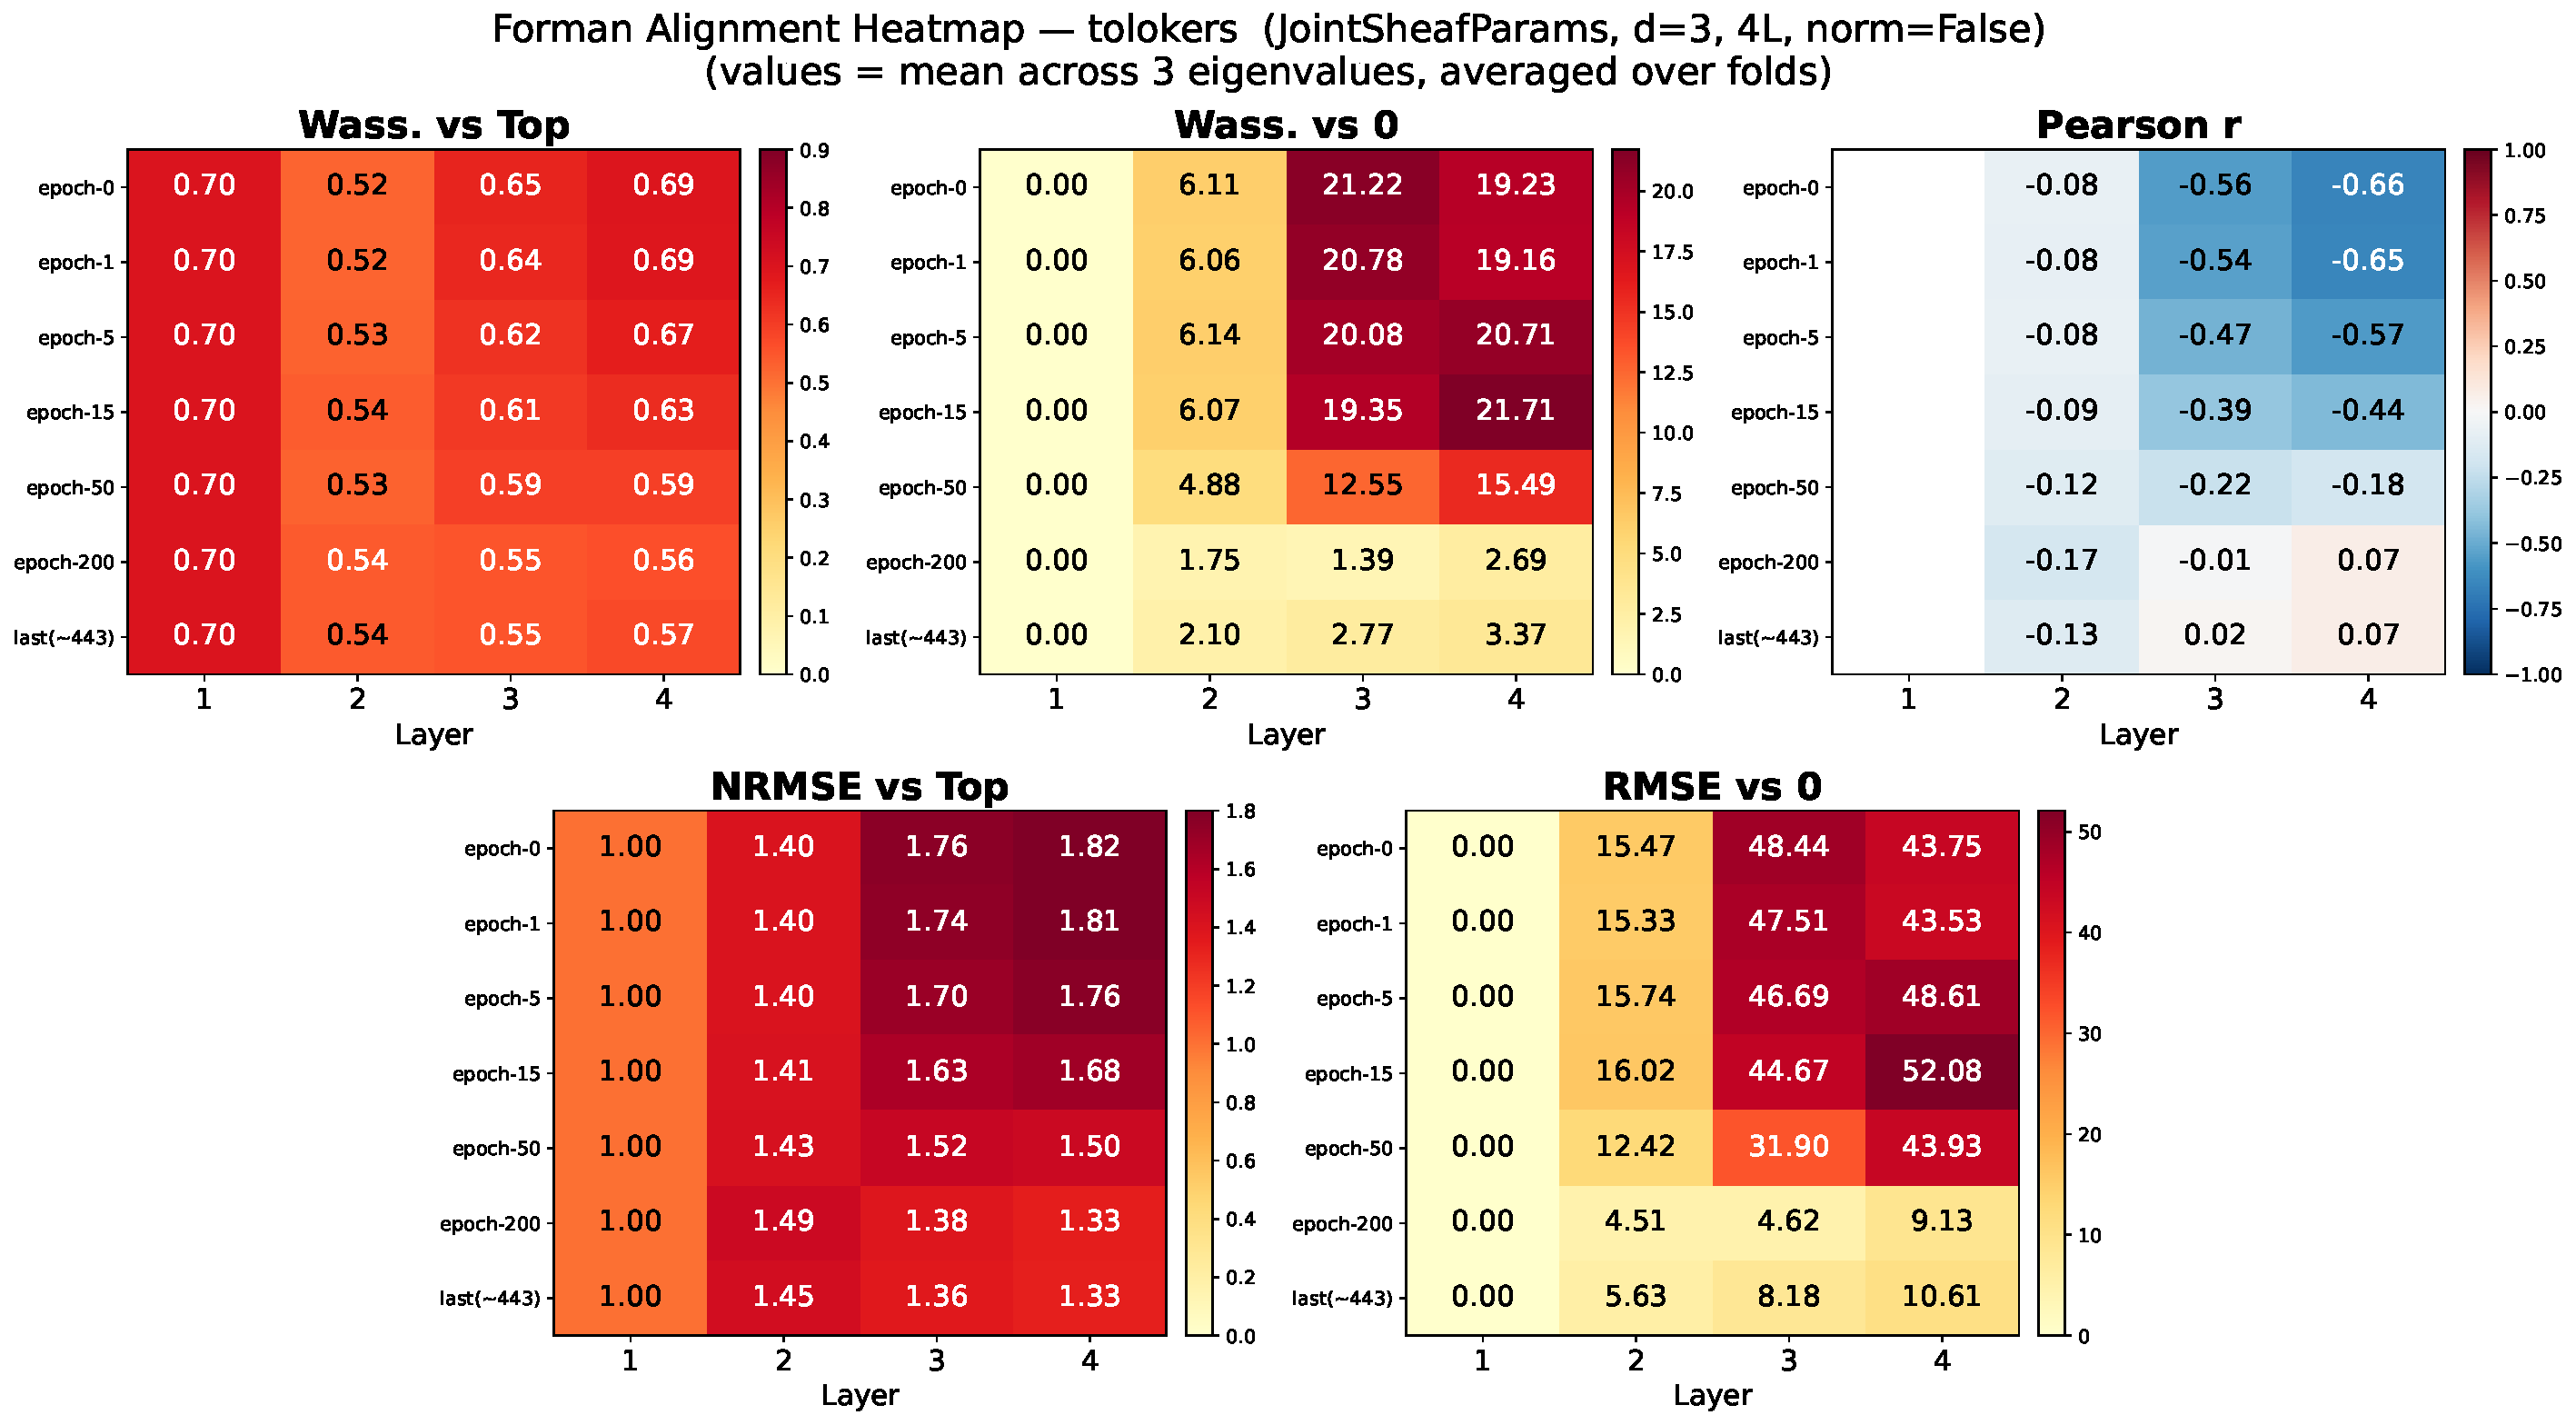
\includegraphics[width=\linewidth]{heatmaps/JointSheafParams/normalised_false/first_maps_identity/tolokers_JointSheafParams_d3_4L_Norm_False_first_maps_identity_heatmap.pdf}
\end{figure}
\end{frame}

\begin{frame}{Wisconsin --- Joint, $d=2$, $L=2$, Norm=False, Identity}
\begin{figure}
    \centering
    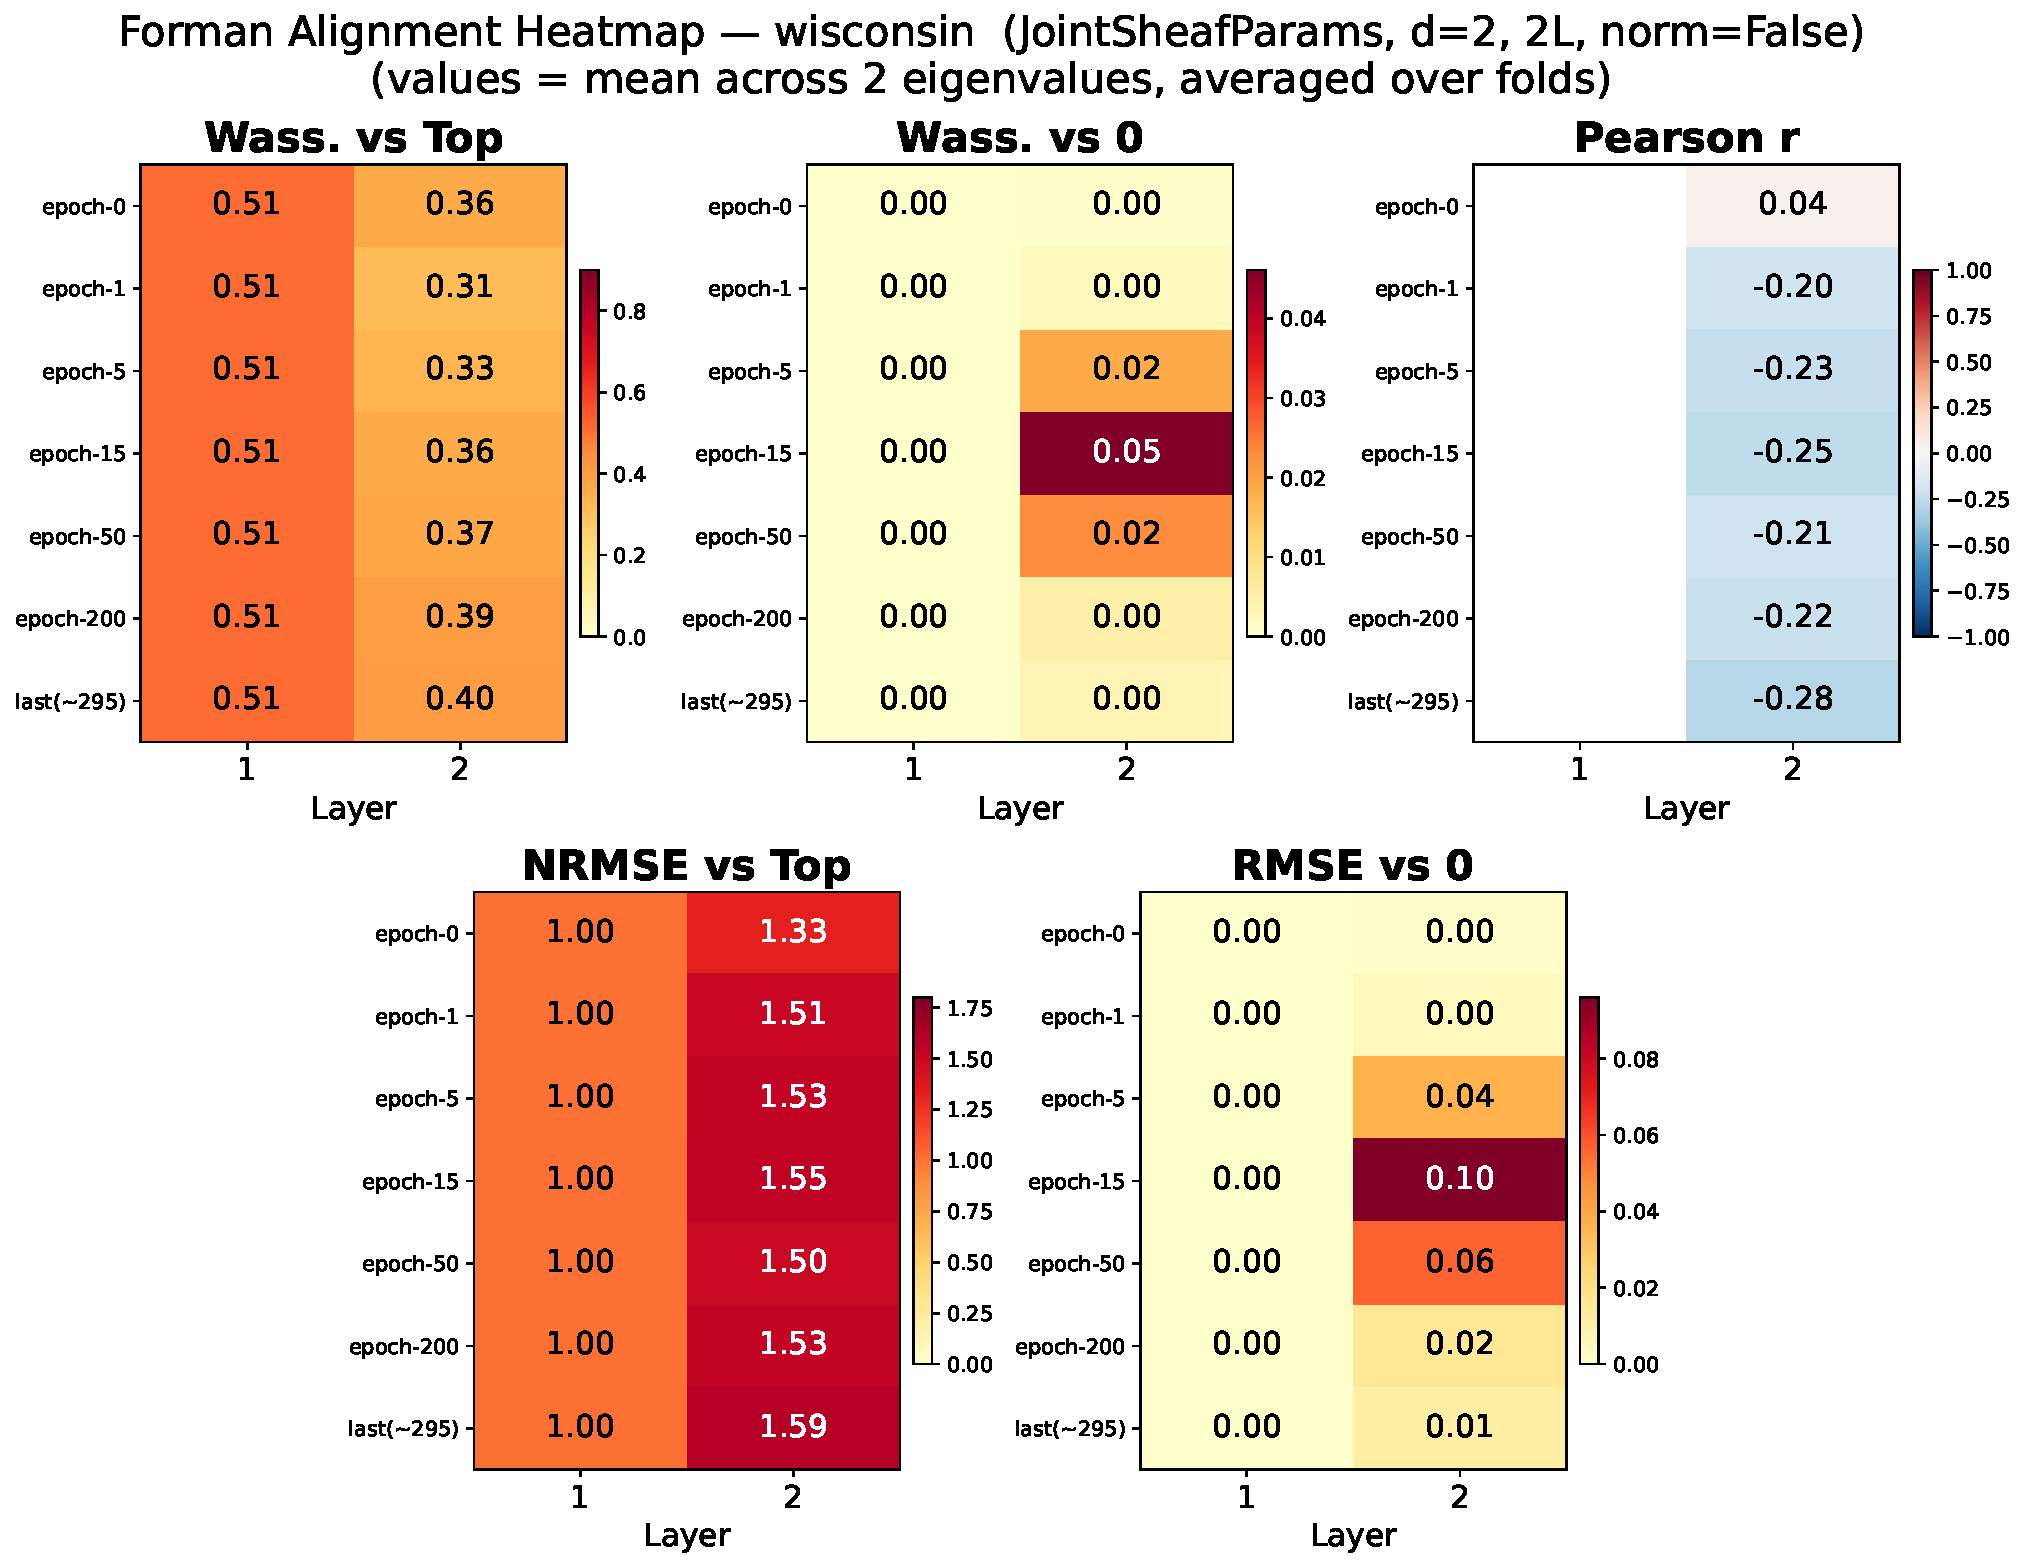
\includegraphics[width=\linewidth]{heatmaps/JointSheafParams/normalised_false/first_maps_identity/wisconsin_JointSheafParams_d2_2L_Norm_False_first_maps_identity_heatmap.pdf}
\end{figure}
\end{frame}

% ══════════════════════════════════════════════════════════════════════════════
%  SECTION 6 — JointSheafParams, normalised=True, identity maps
% ══════════════════════════════════════════════════════════════════════════════

\begin{frame}{}
\centering
\Huge\textbf{JointSheafParams}\\[6pt]
\Large Norm=True, Identity Initial Maps
\end{frame}

\begin{frame}{Amazon Ratings --- Joint, $d=2$, $L=3$, Norm=True, Identity}
\begin{figure}
    \centering
    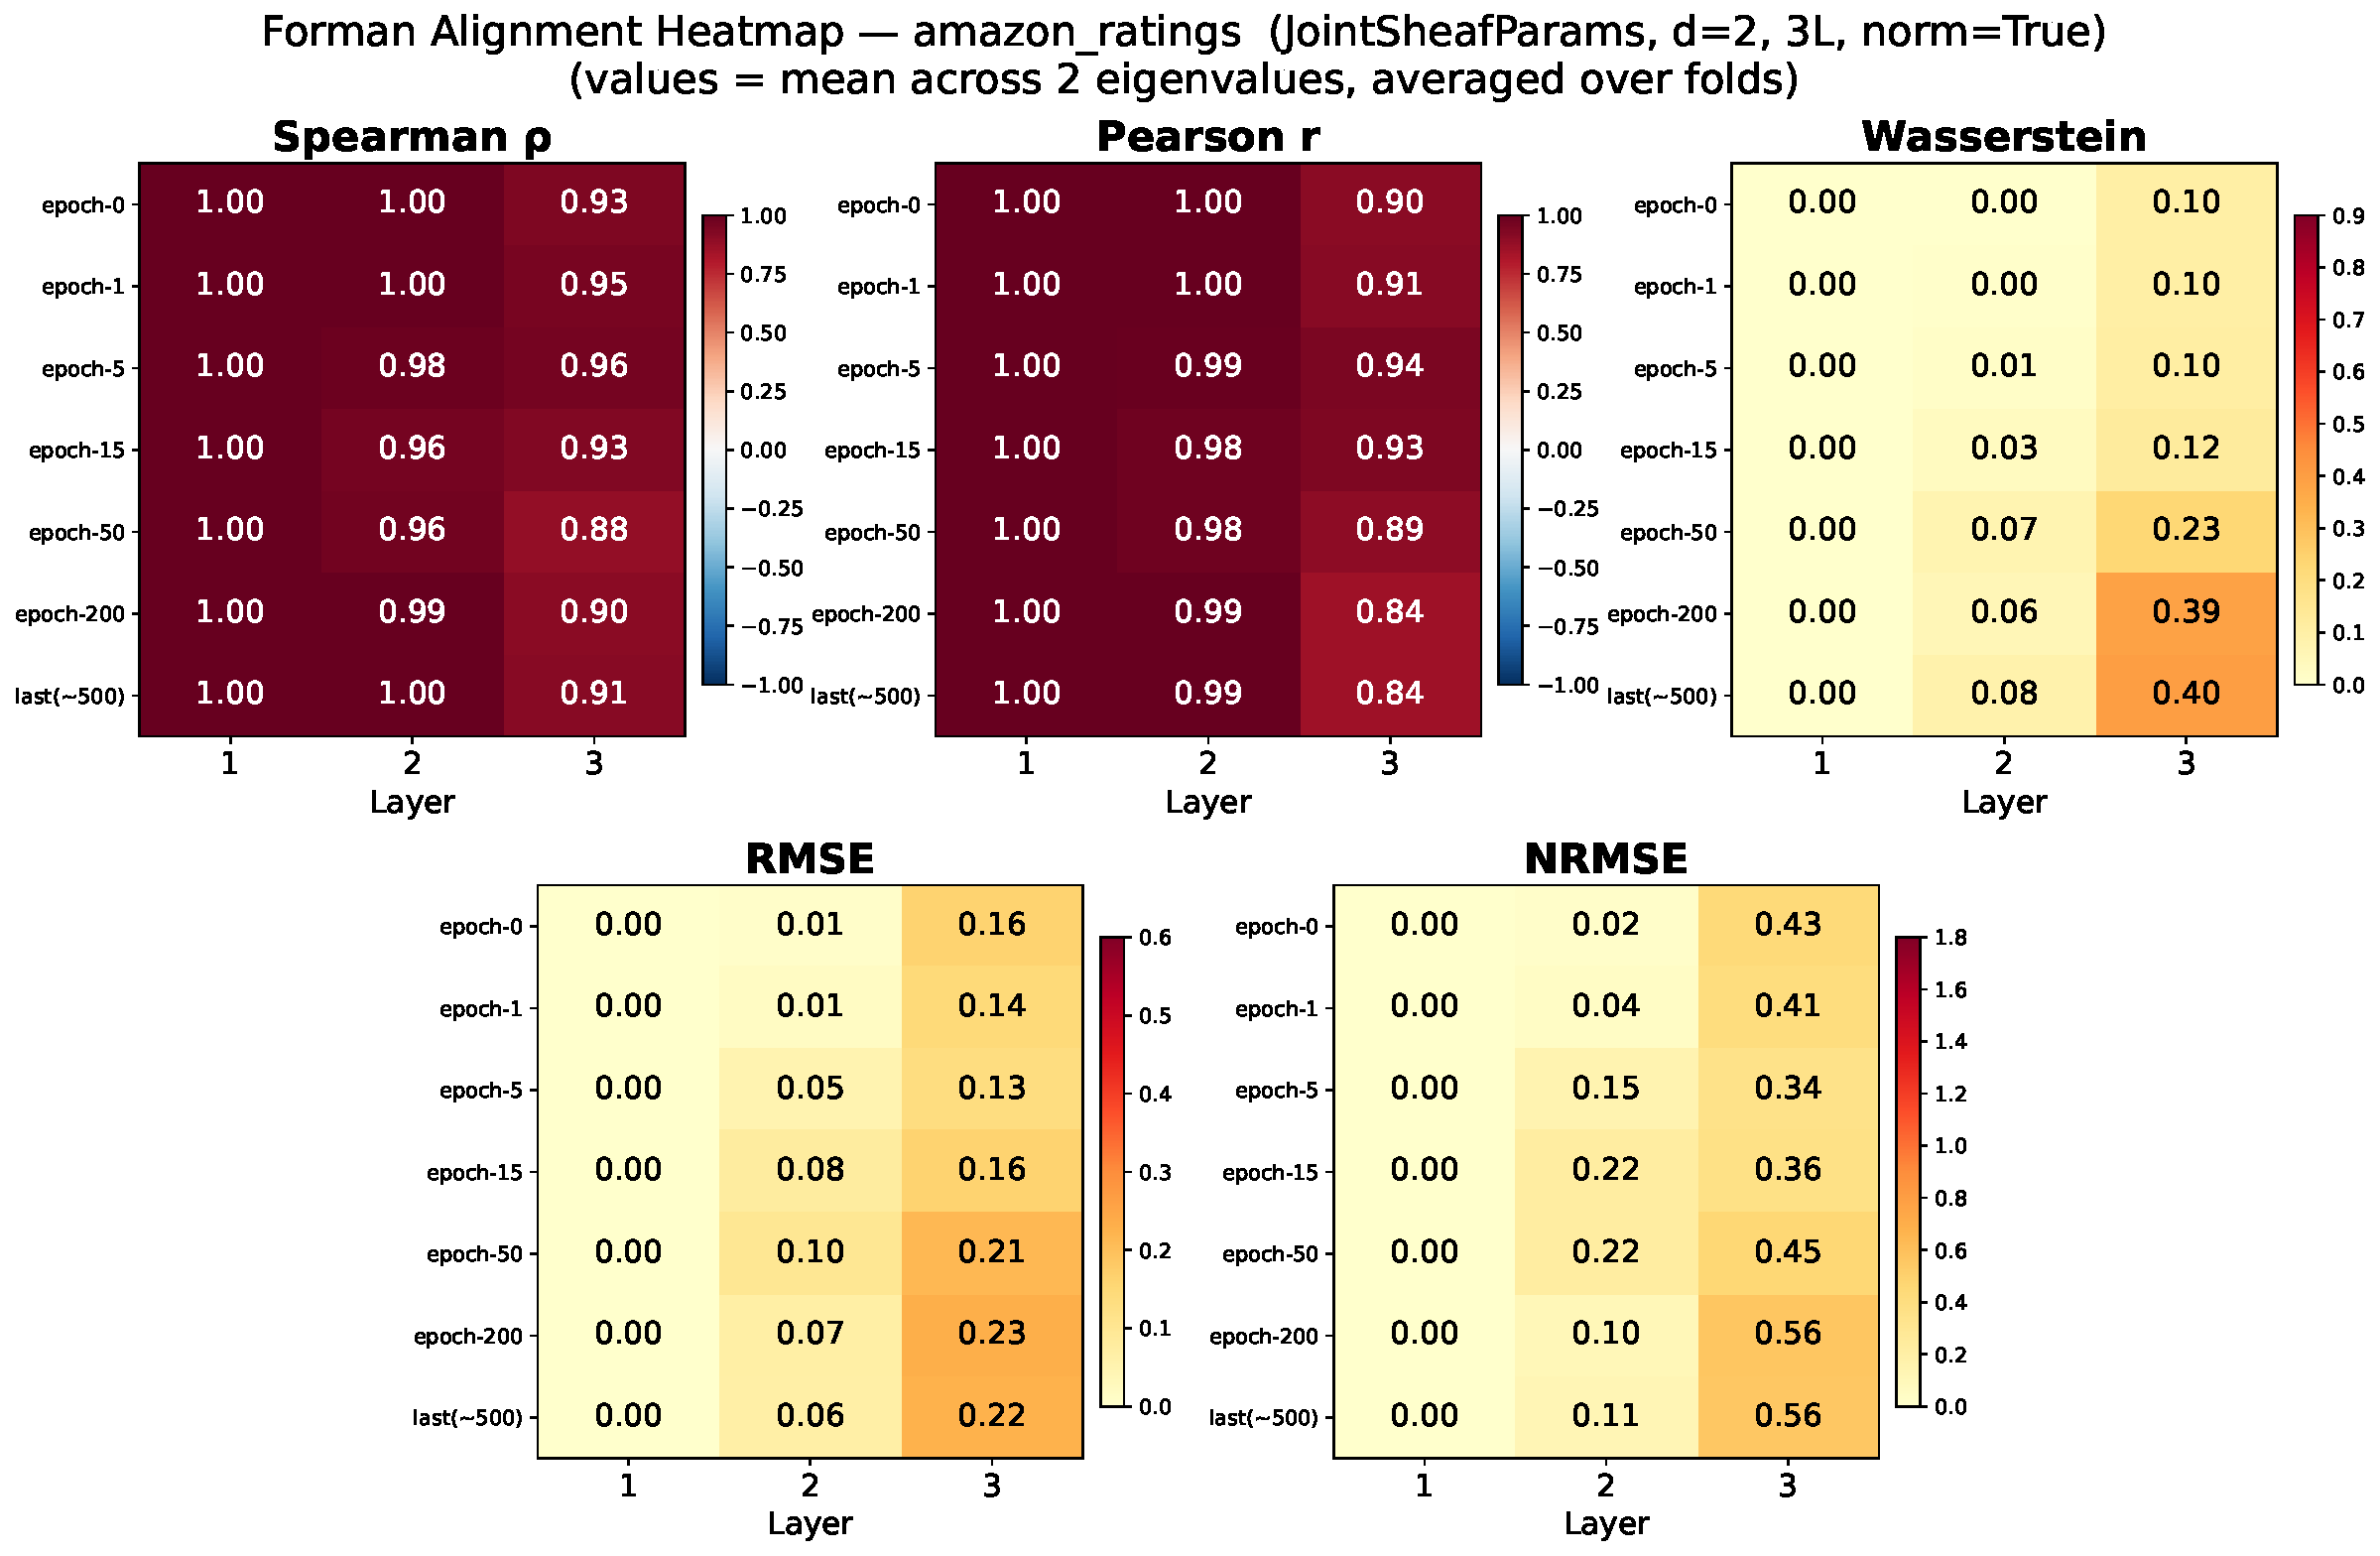
\includegraphics[width=\linewidth]{heatmaps/JointSheafParams/normalised_true/first_maps_identity/amazon_ratings_JointSheafParams_d2_3L_Norm_True_first_maps_identity_heatmap.pdf}
\end{figure}
\end{frame}

\begin{frame}{Citeseer --- Joint, $d=3$, $L=3$, Norm=True, Identity}
\begin{figure}
    \centering
    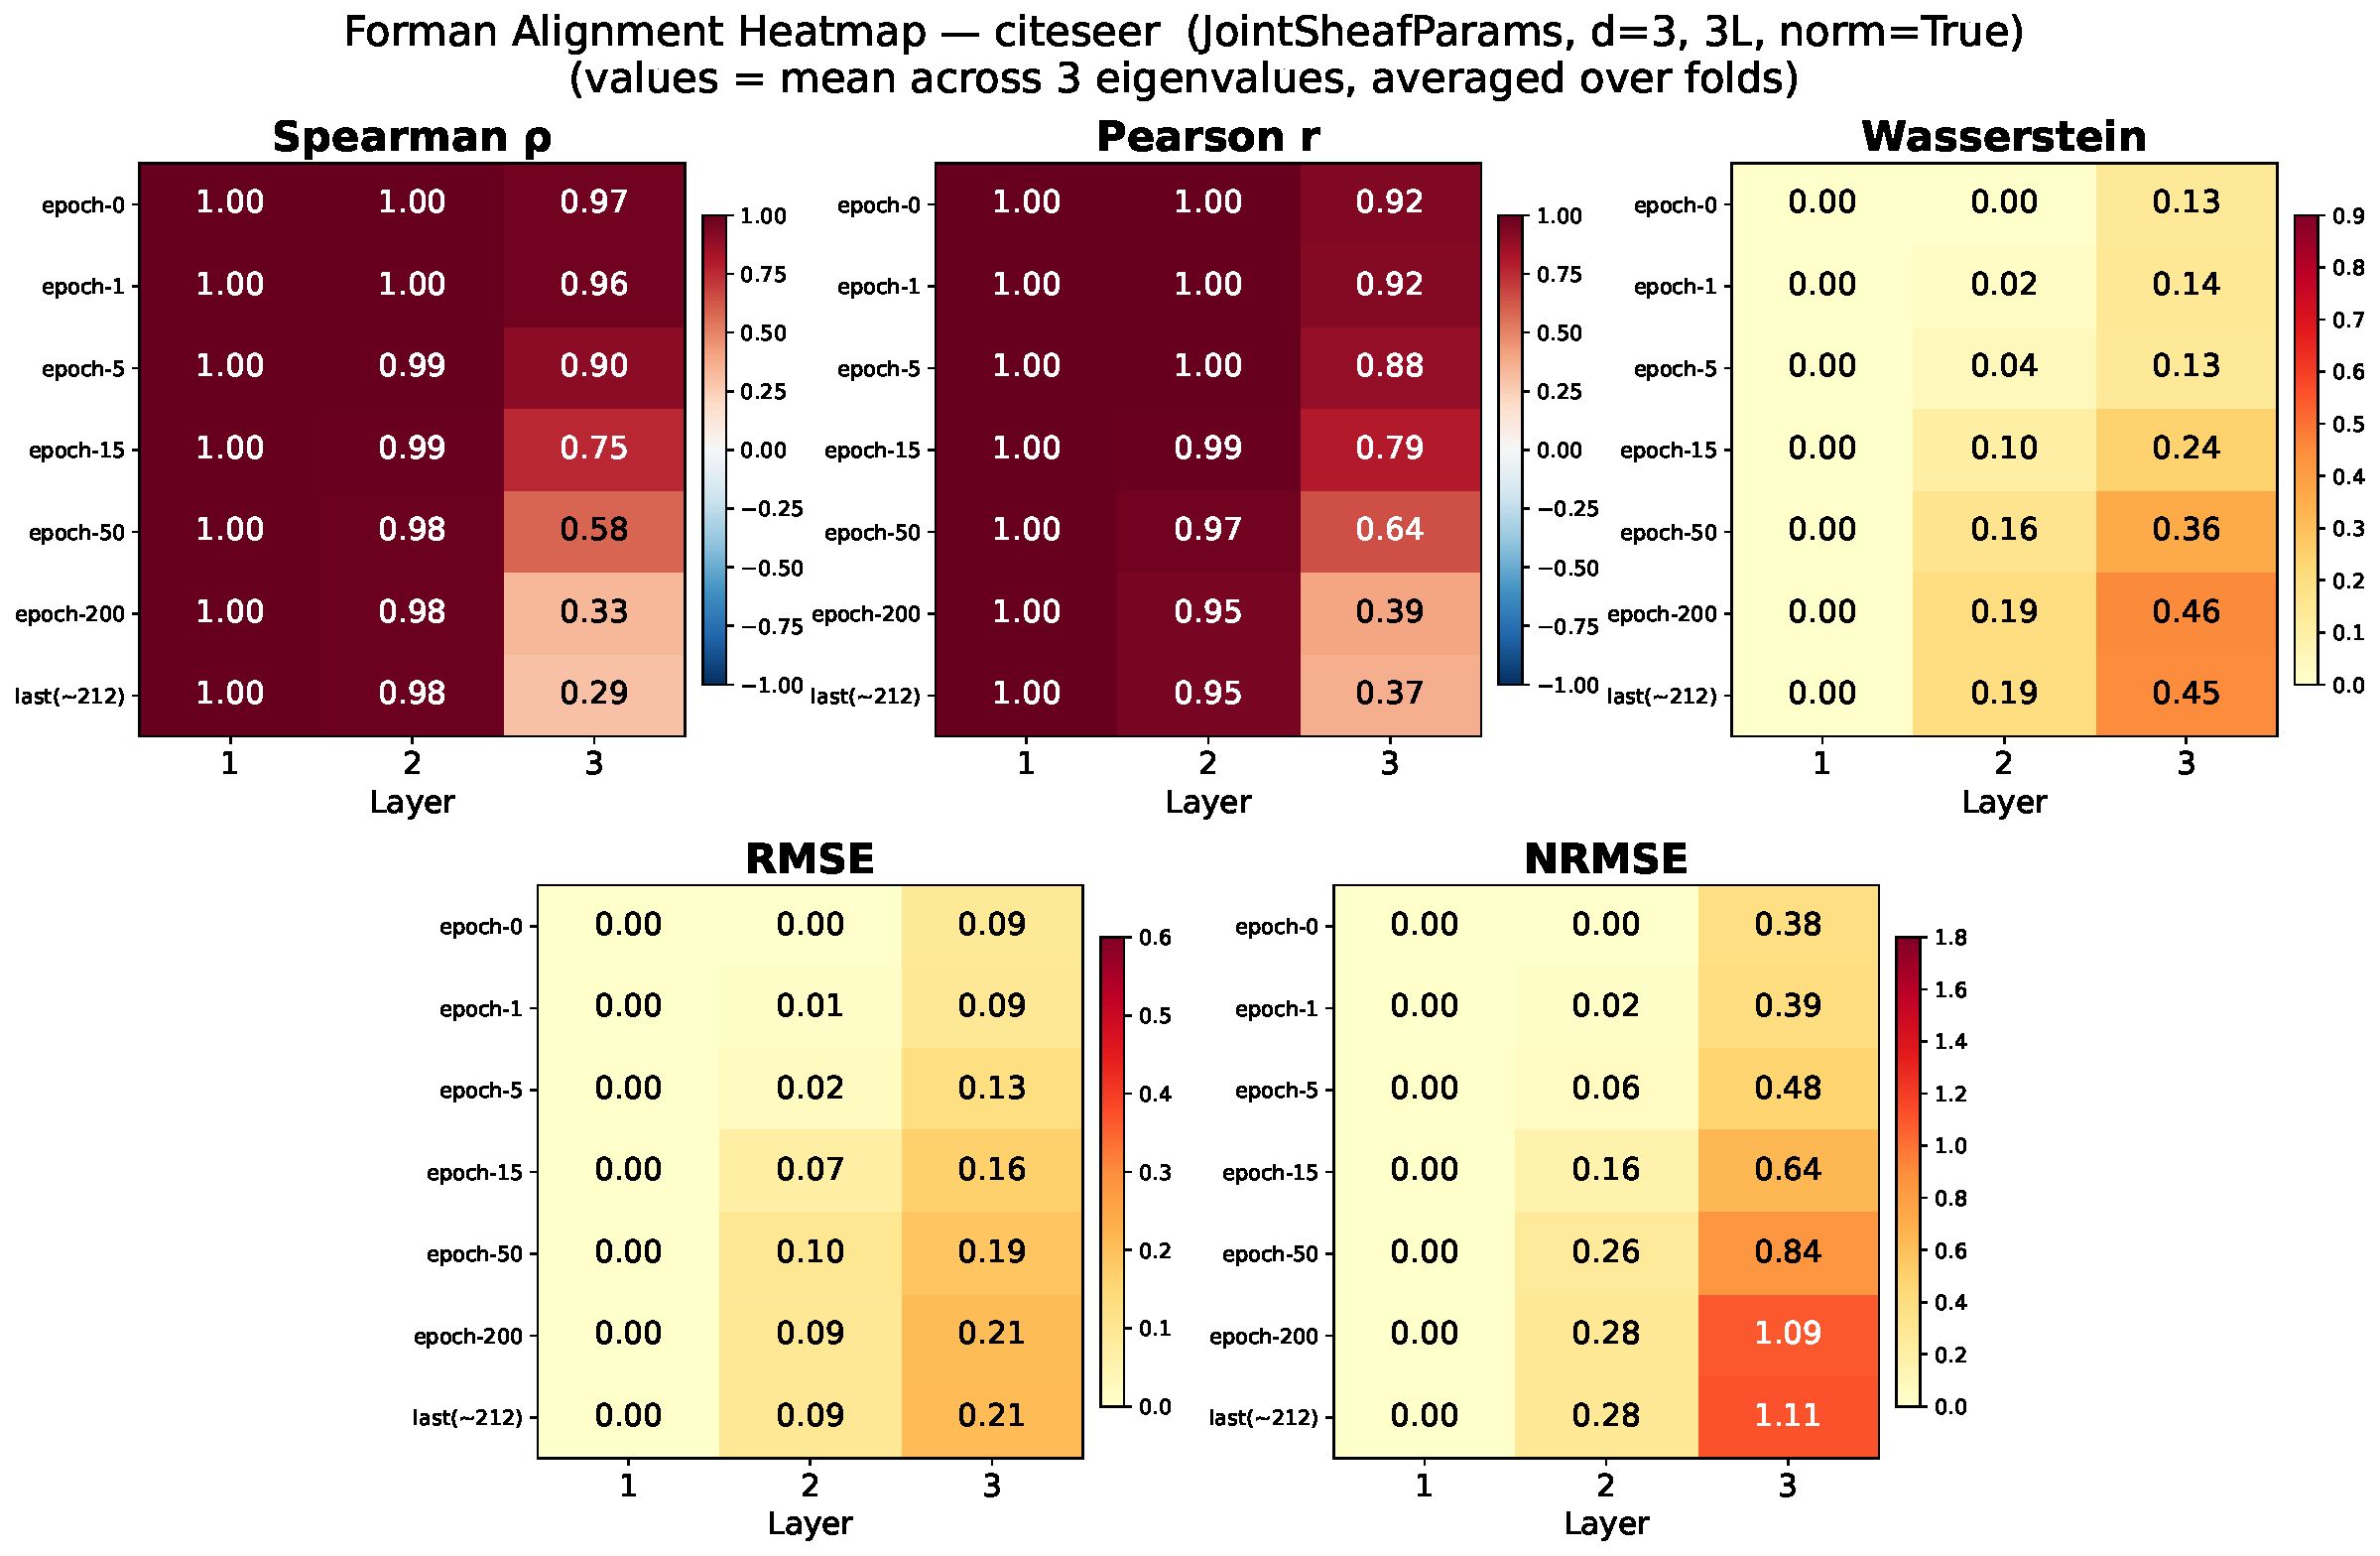
\includegraphics[width=\linewidth]{heatmaps/JointSheafParams/normalised_true/first_maps_identity/citeseer_JointSheafParams_d3_3L_Norm_True_first_maps_identity_heatmap.pdf}
\end{figure}
\end{frame}

\begin{frame}{Cora --- Joint, $d=2$, $L=3$, Norm=True, Identity}
\begin{figure}
    \centering
    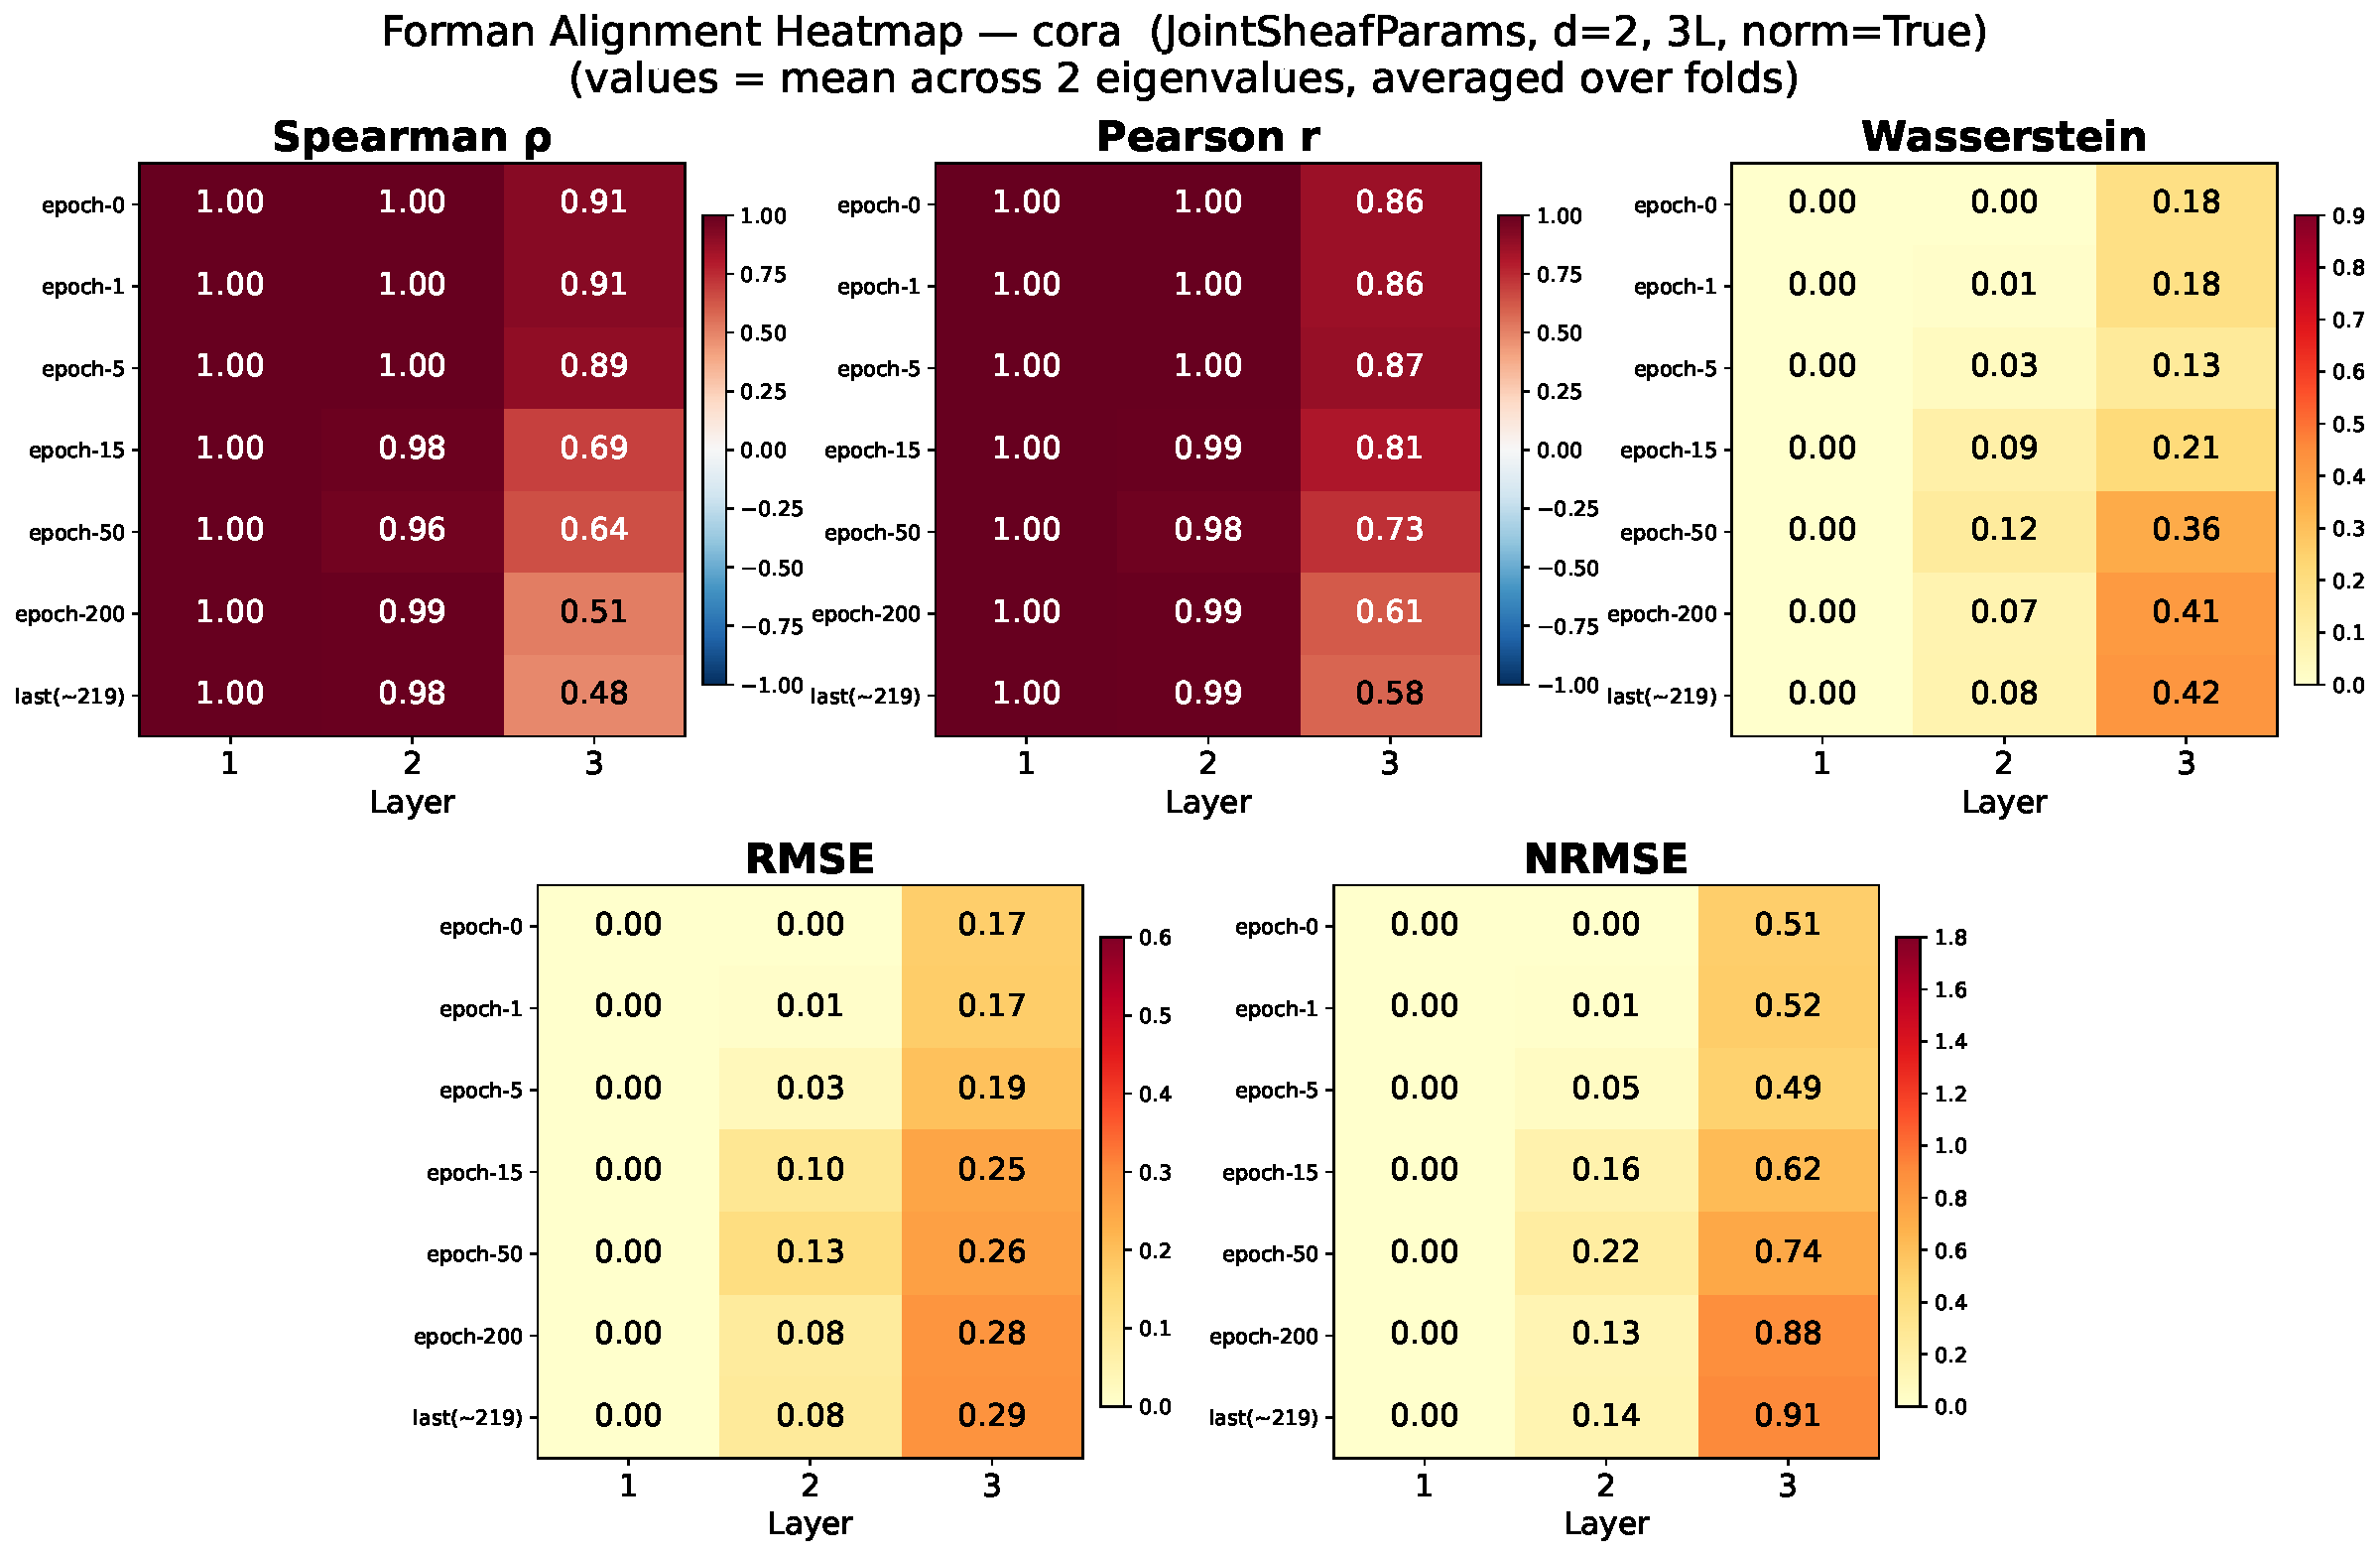
\includegraphics[width=\linewidth]{heatmaps/JointSheafParams/normalised_true/first_maps_identity/cora_JointSheafParams_d2_3L_Norm_True_first_maps_identity_heatmap.pdf}
\end{figure}
\end{frame}

\begin{frame}{Cora --- Joint, $d=3$, $L=3$, Norm=True, Identity}
\begin{figure}
    \centering
    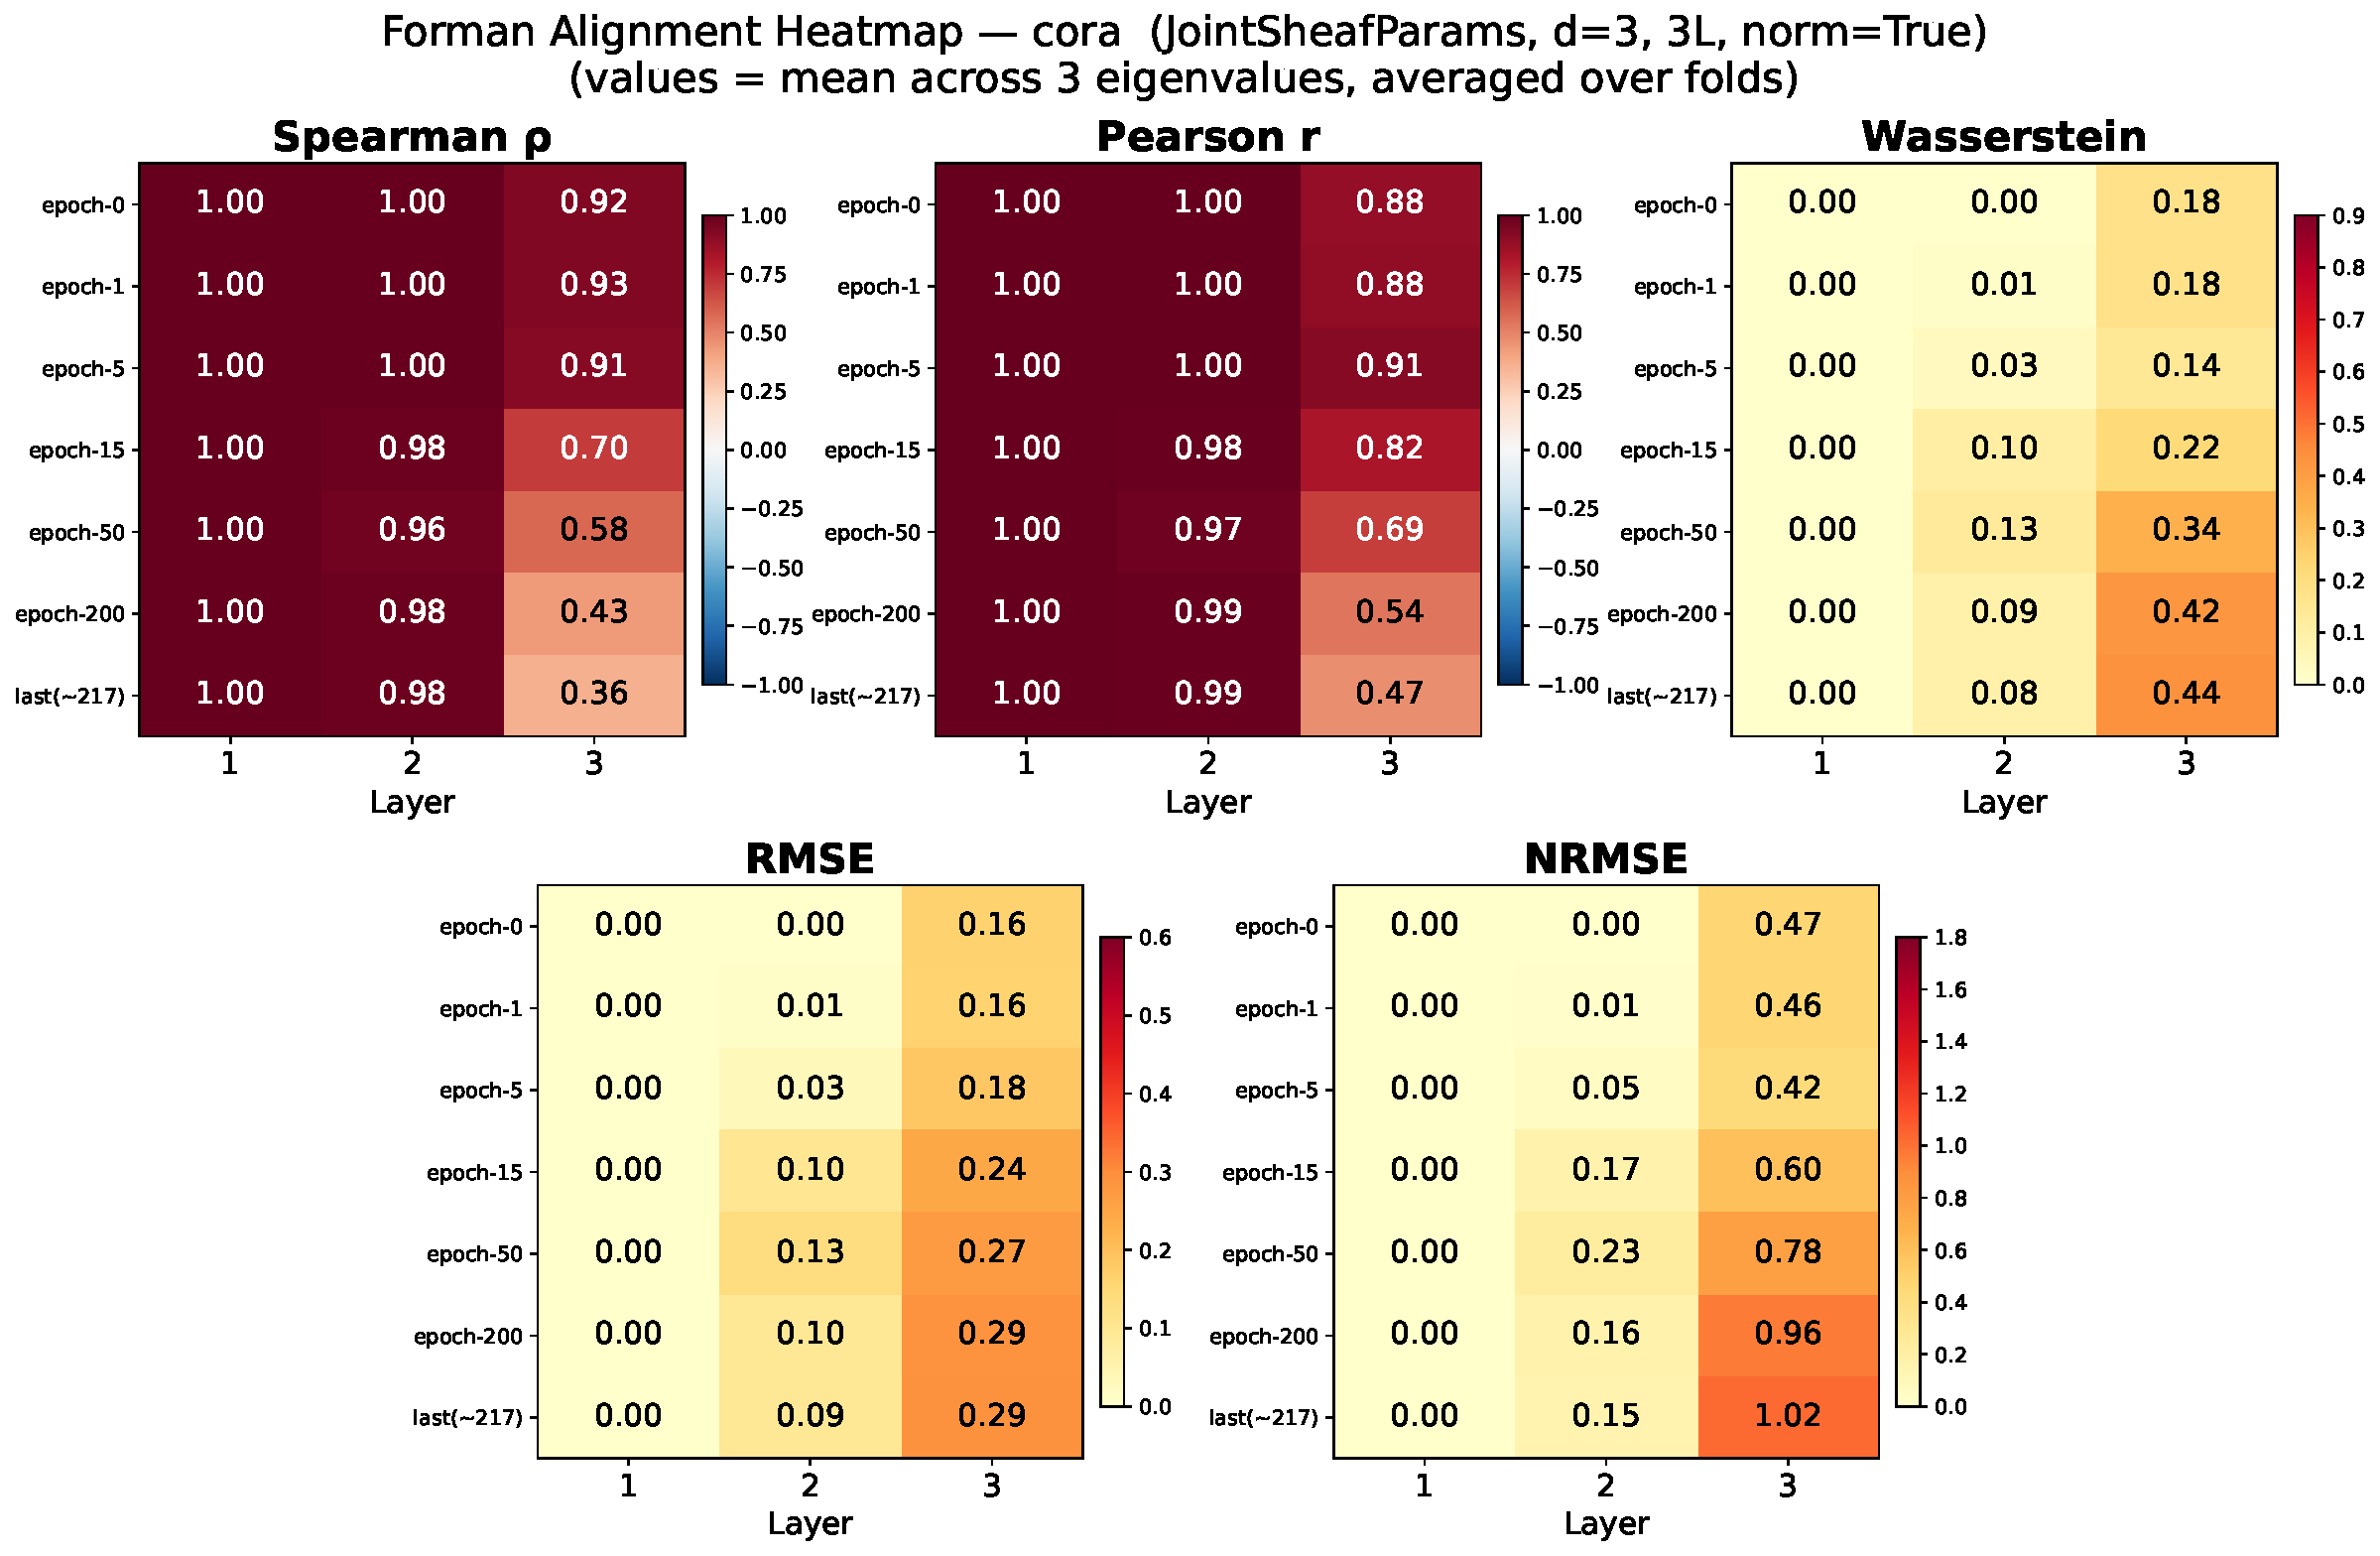
\includegraphics[width=\linewidth]{heatmaps/JointSheafParams/normalised_true/first_maps_identity/cora_JointSheafParams_d3_3L_Norm_True_first_maps_identity_heatmap.pdf}
\end{figure}
\end{frame}

\begin{frame}{Cornell --- Joint, $d=2$, $L=2$, Norm=True, Identity}
\begin{figure}
    \centering
    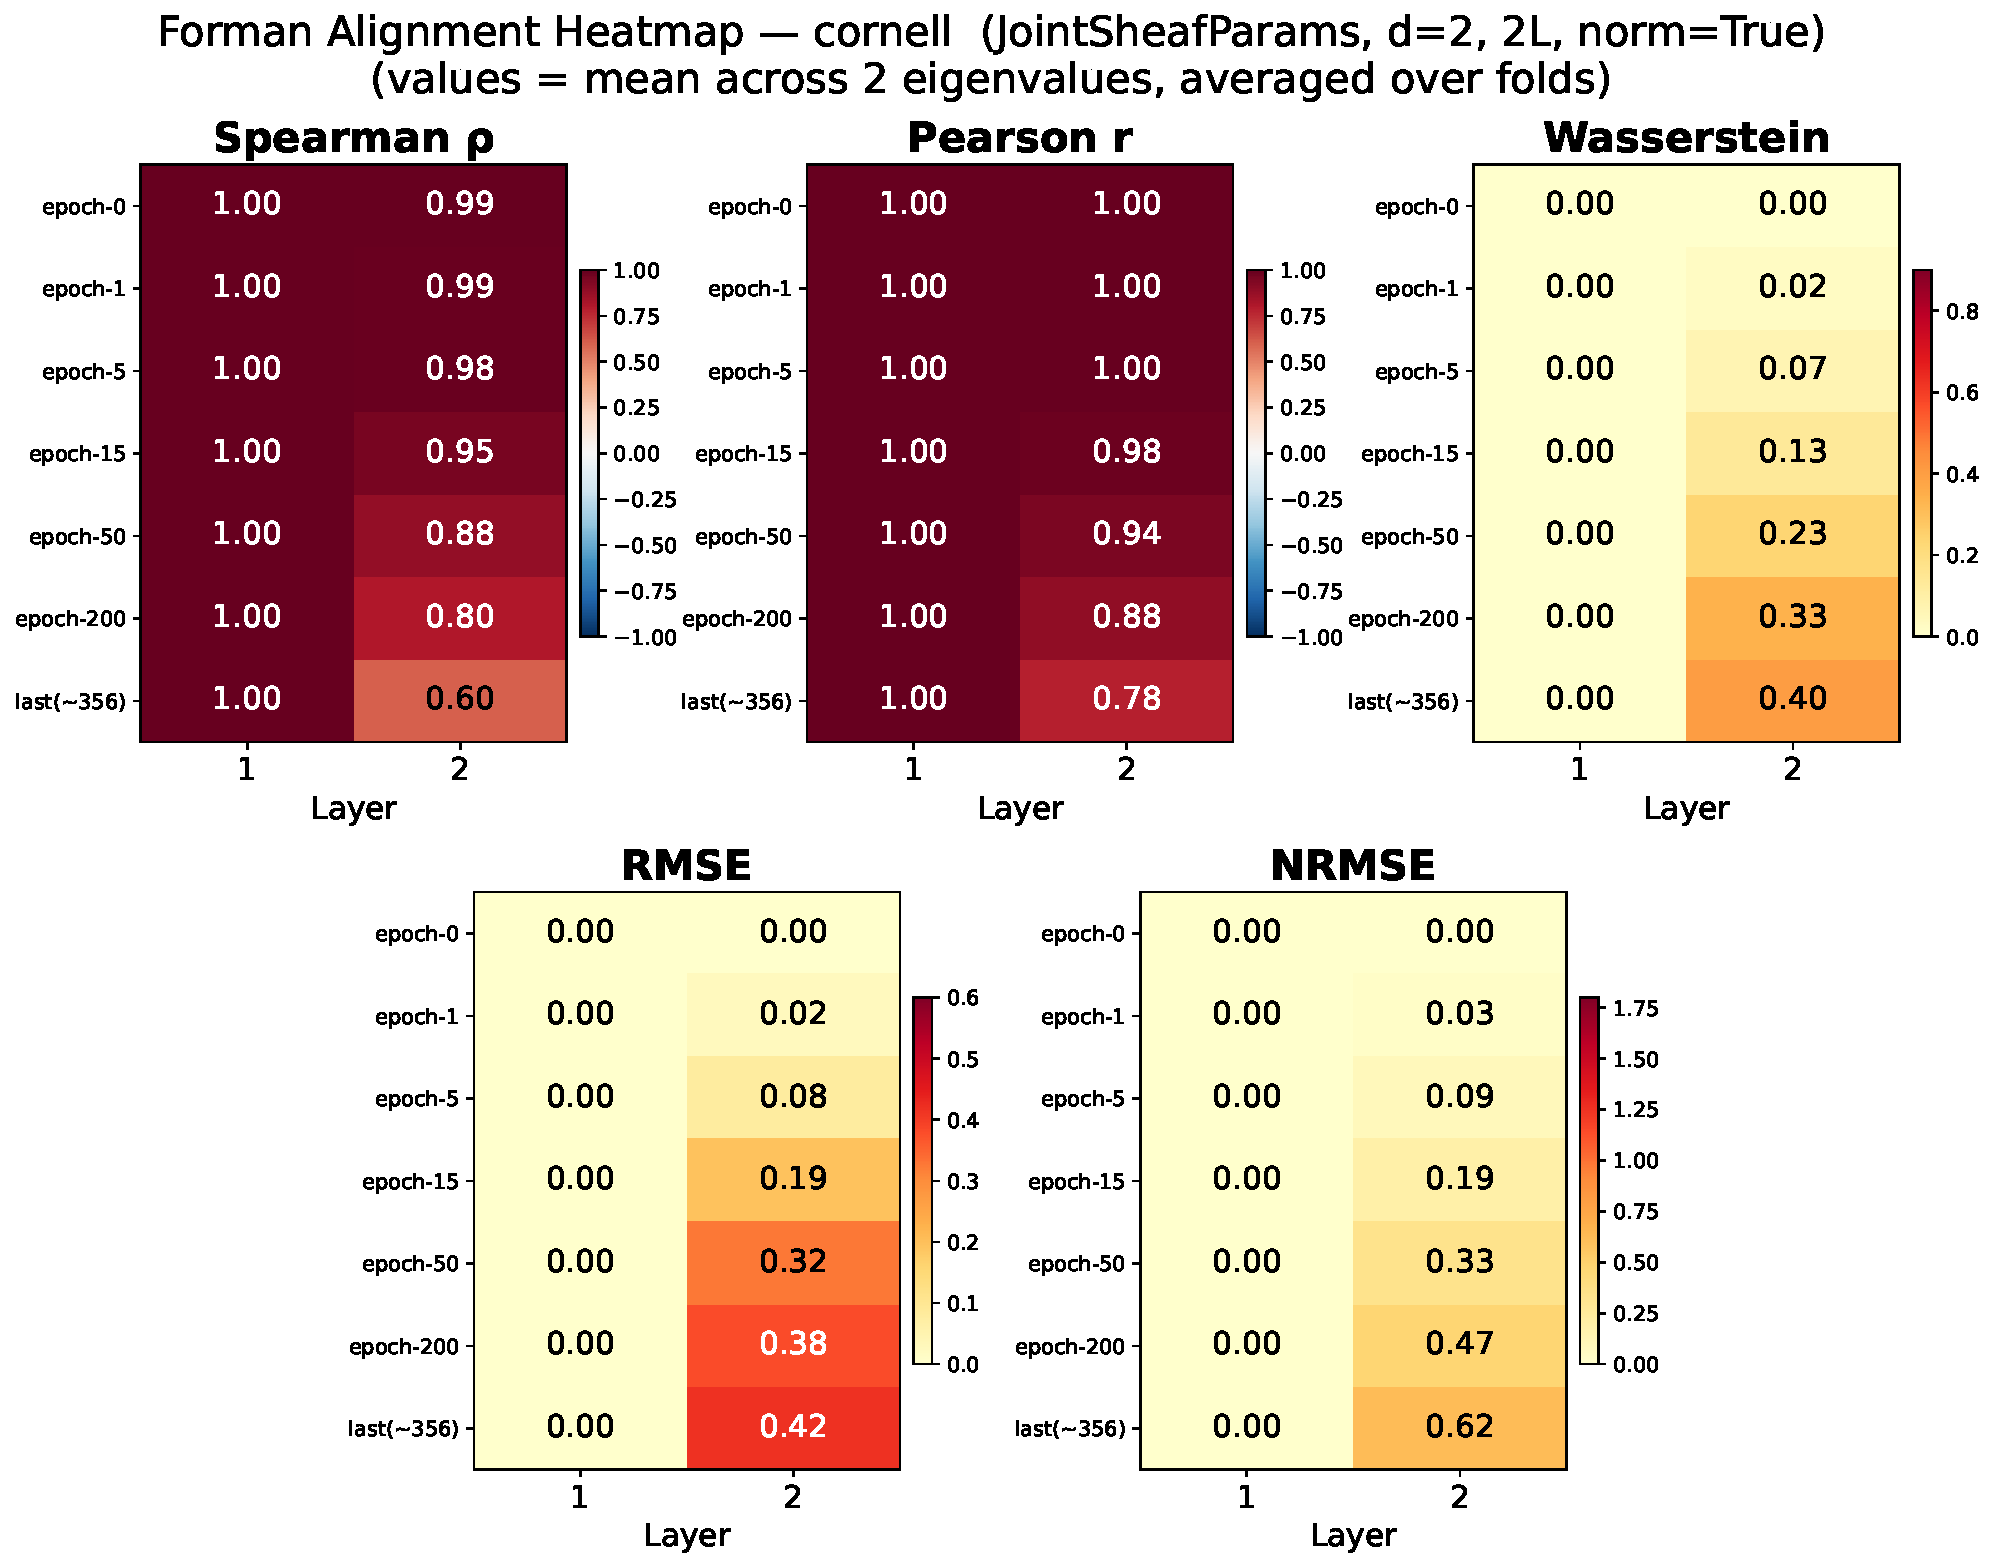
\includegraphics[width=\linewidth]{heatmaps/JointSheafParams/normalised_true/first_maps_identity/cornell_JointSheafParams_d2_2L_Norm_True_first_maps_identity_heatmap.pdf}
\end{figure}
\end{frame}

\begin{frame}{Minesweeper --- Joint, $d=3$, $L=3$, Norm=True, Identity}
\begin{figure}
    \centering
    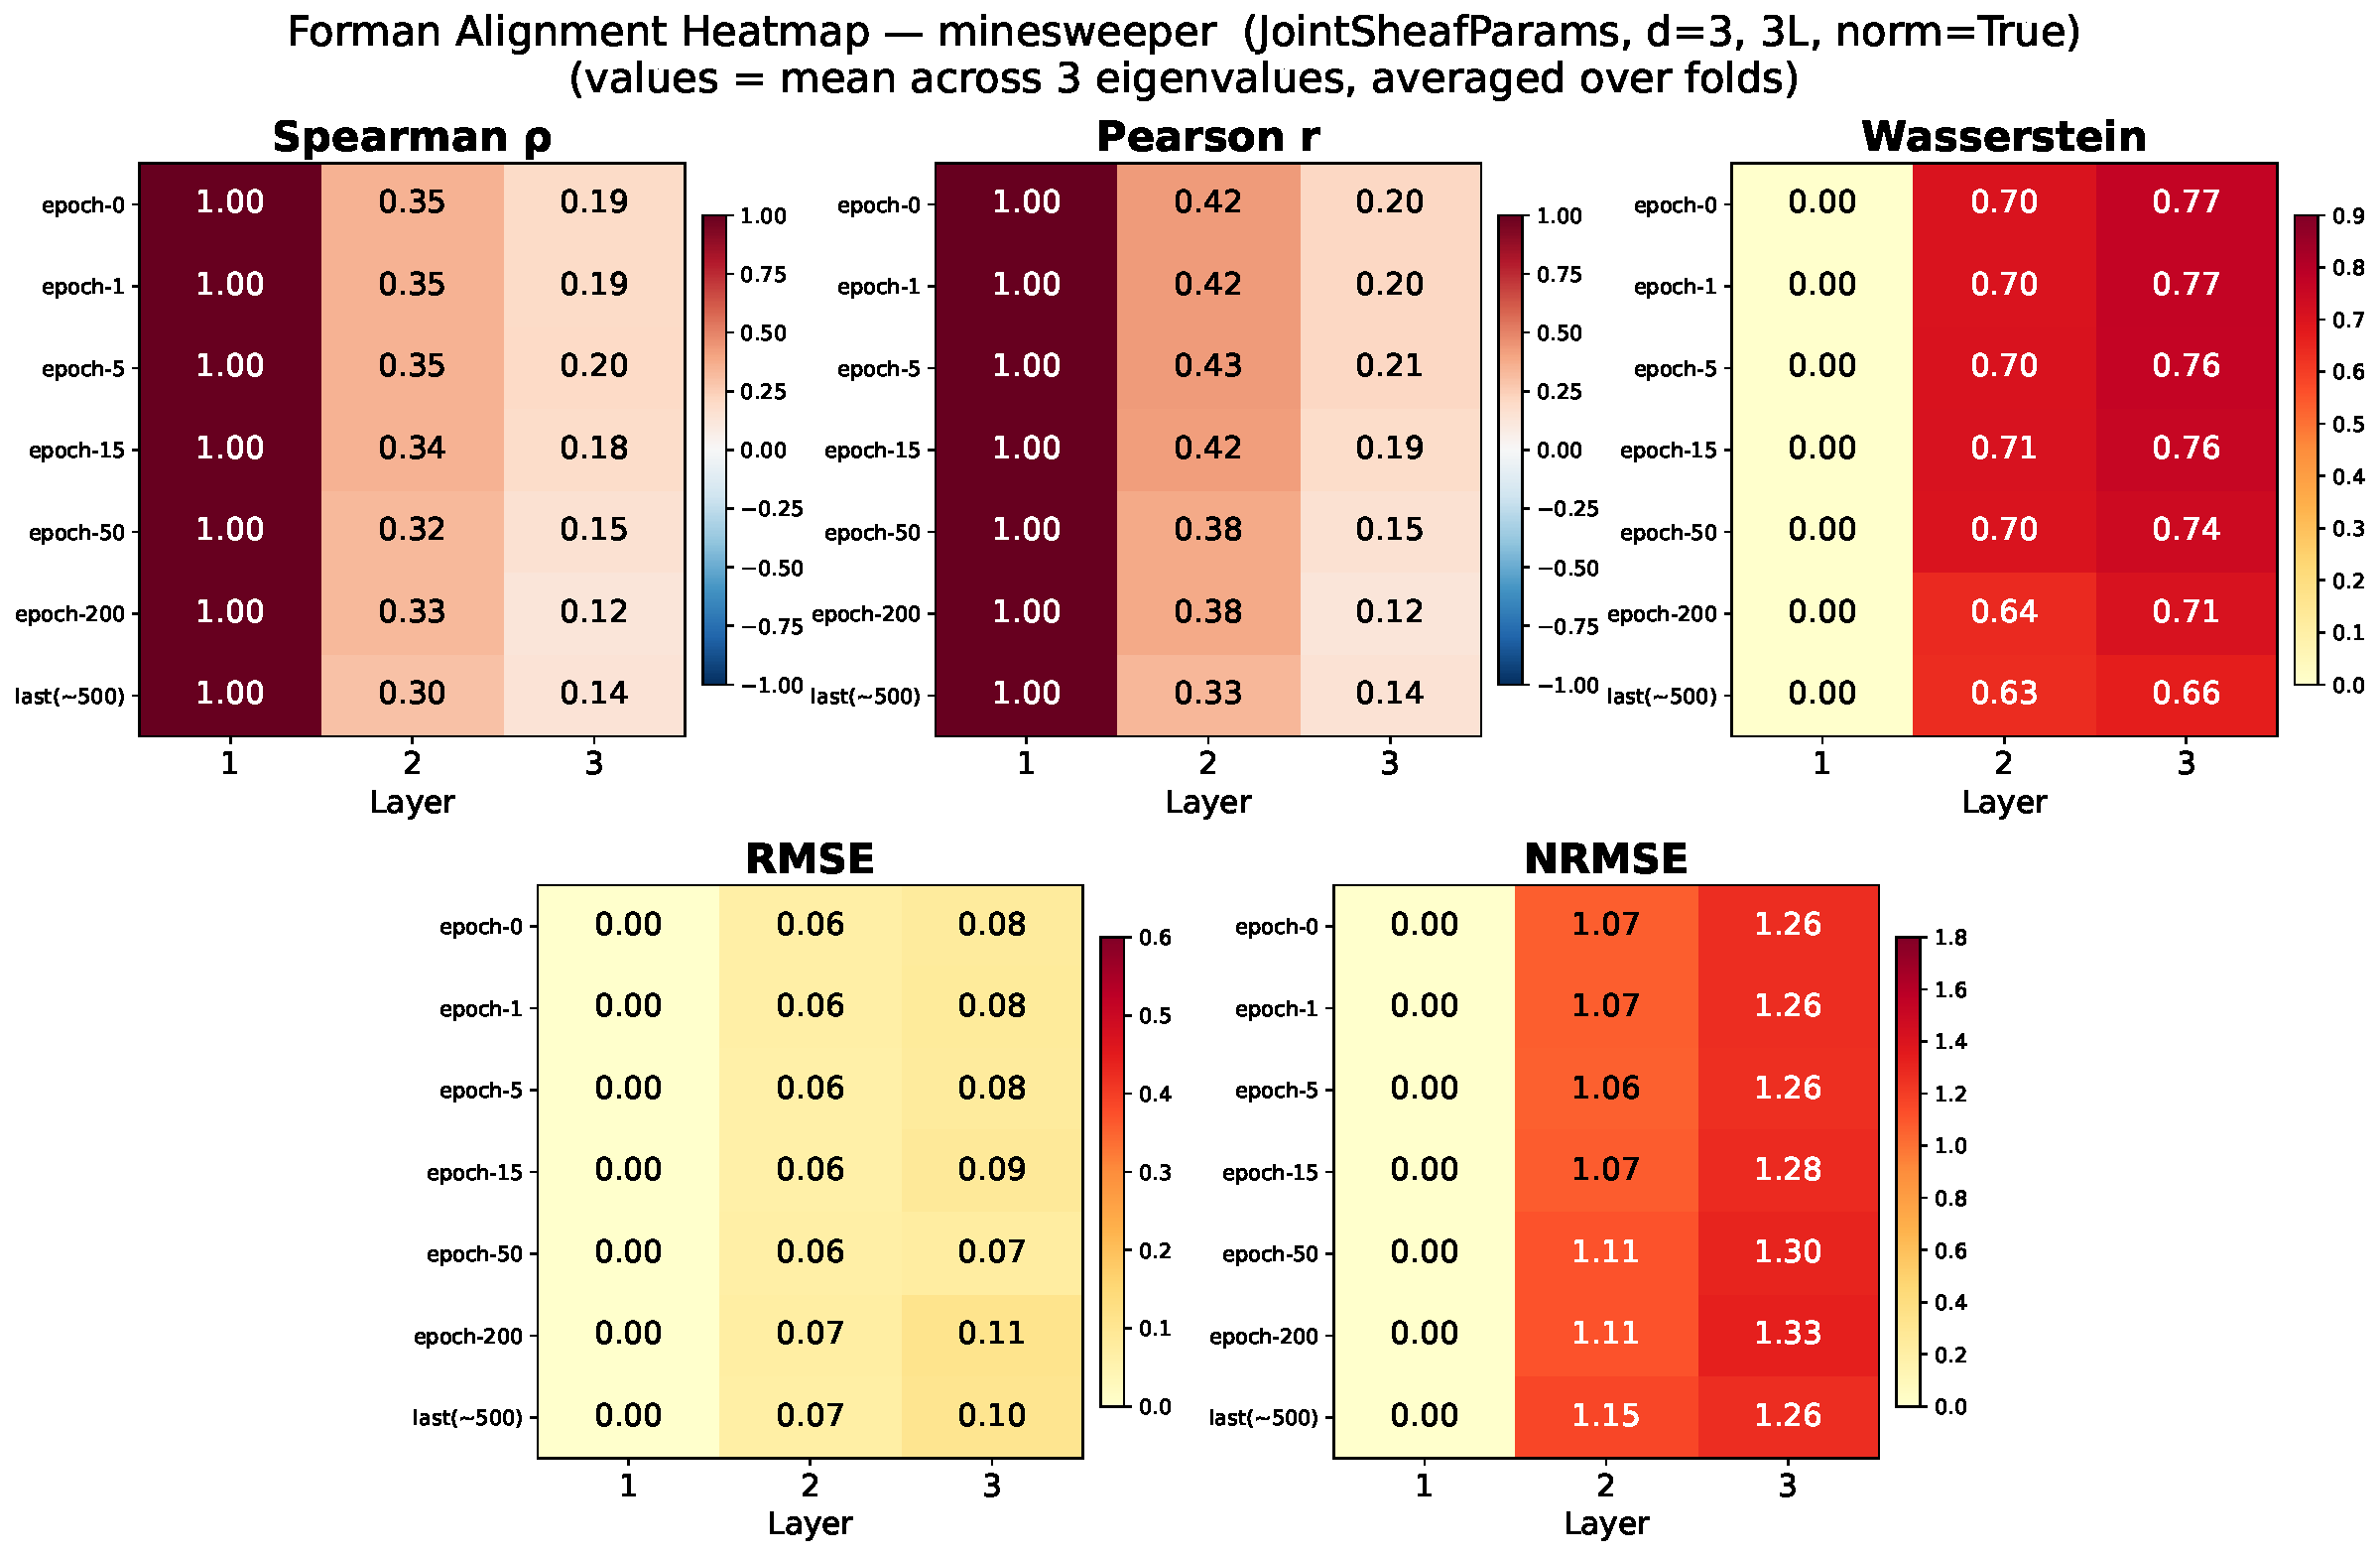
\includegraphics[width=\linewidth]{heatmaps/JointSheafParams/normalised_true/first_maps_identity/minesweeper_JointSheafParams_d3_3L_Norm_True_first_maps_identity_heatmap.pdf}
\end{figure}
\end{frame}

\begin{frame}{Pubmed --- Joint, $d=2$, $L=3$, Norm=True, Identity}
\begin{figure}
    \centering
    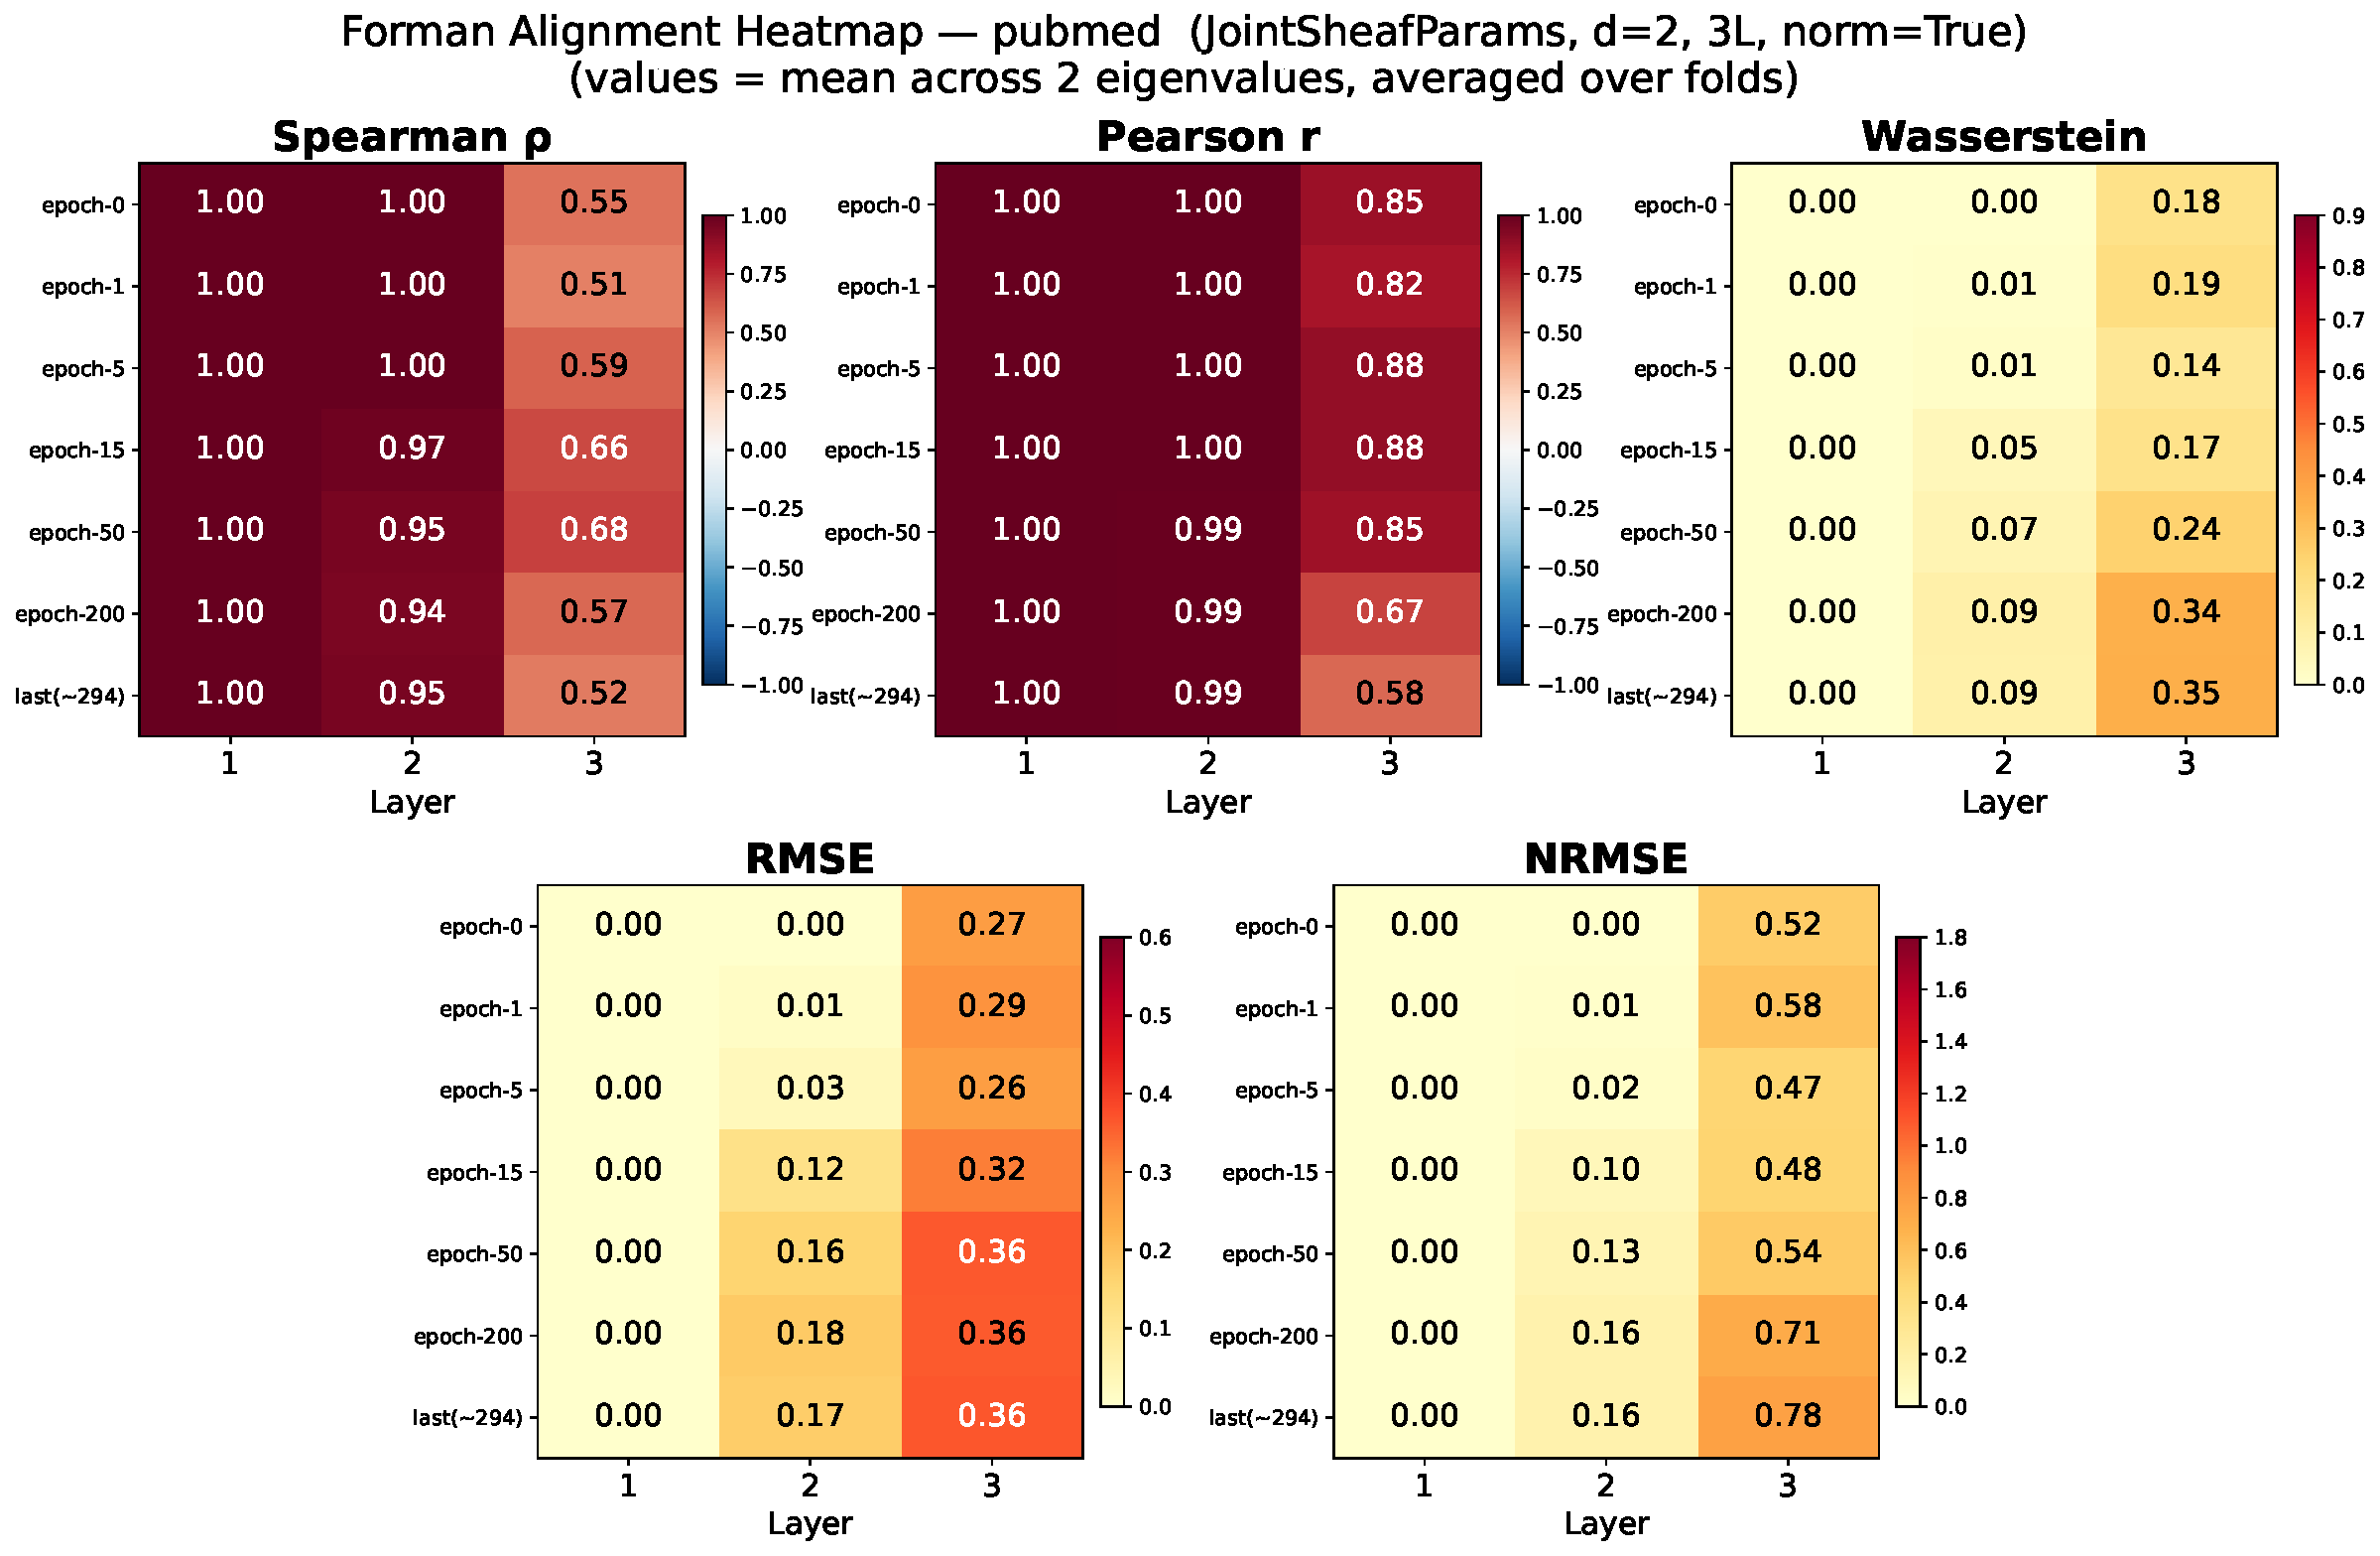
\includegraphics[width=\linewidth]{heatmaps/JointSheafParams/normalised_true/first_maps_identity/pubmed_JointSheafParams_d2_3L_Norm_True_first_maps_identity_heatmap.pdf}
\end{figure}
\end{frame}

\begin{frame}{Pubmed --- Joint, $d=3$, $L=3$, Norm=True, Identity}
\begin{figure}
    \centering
    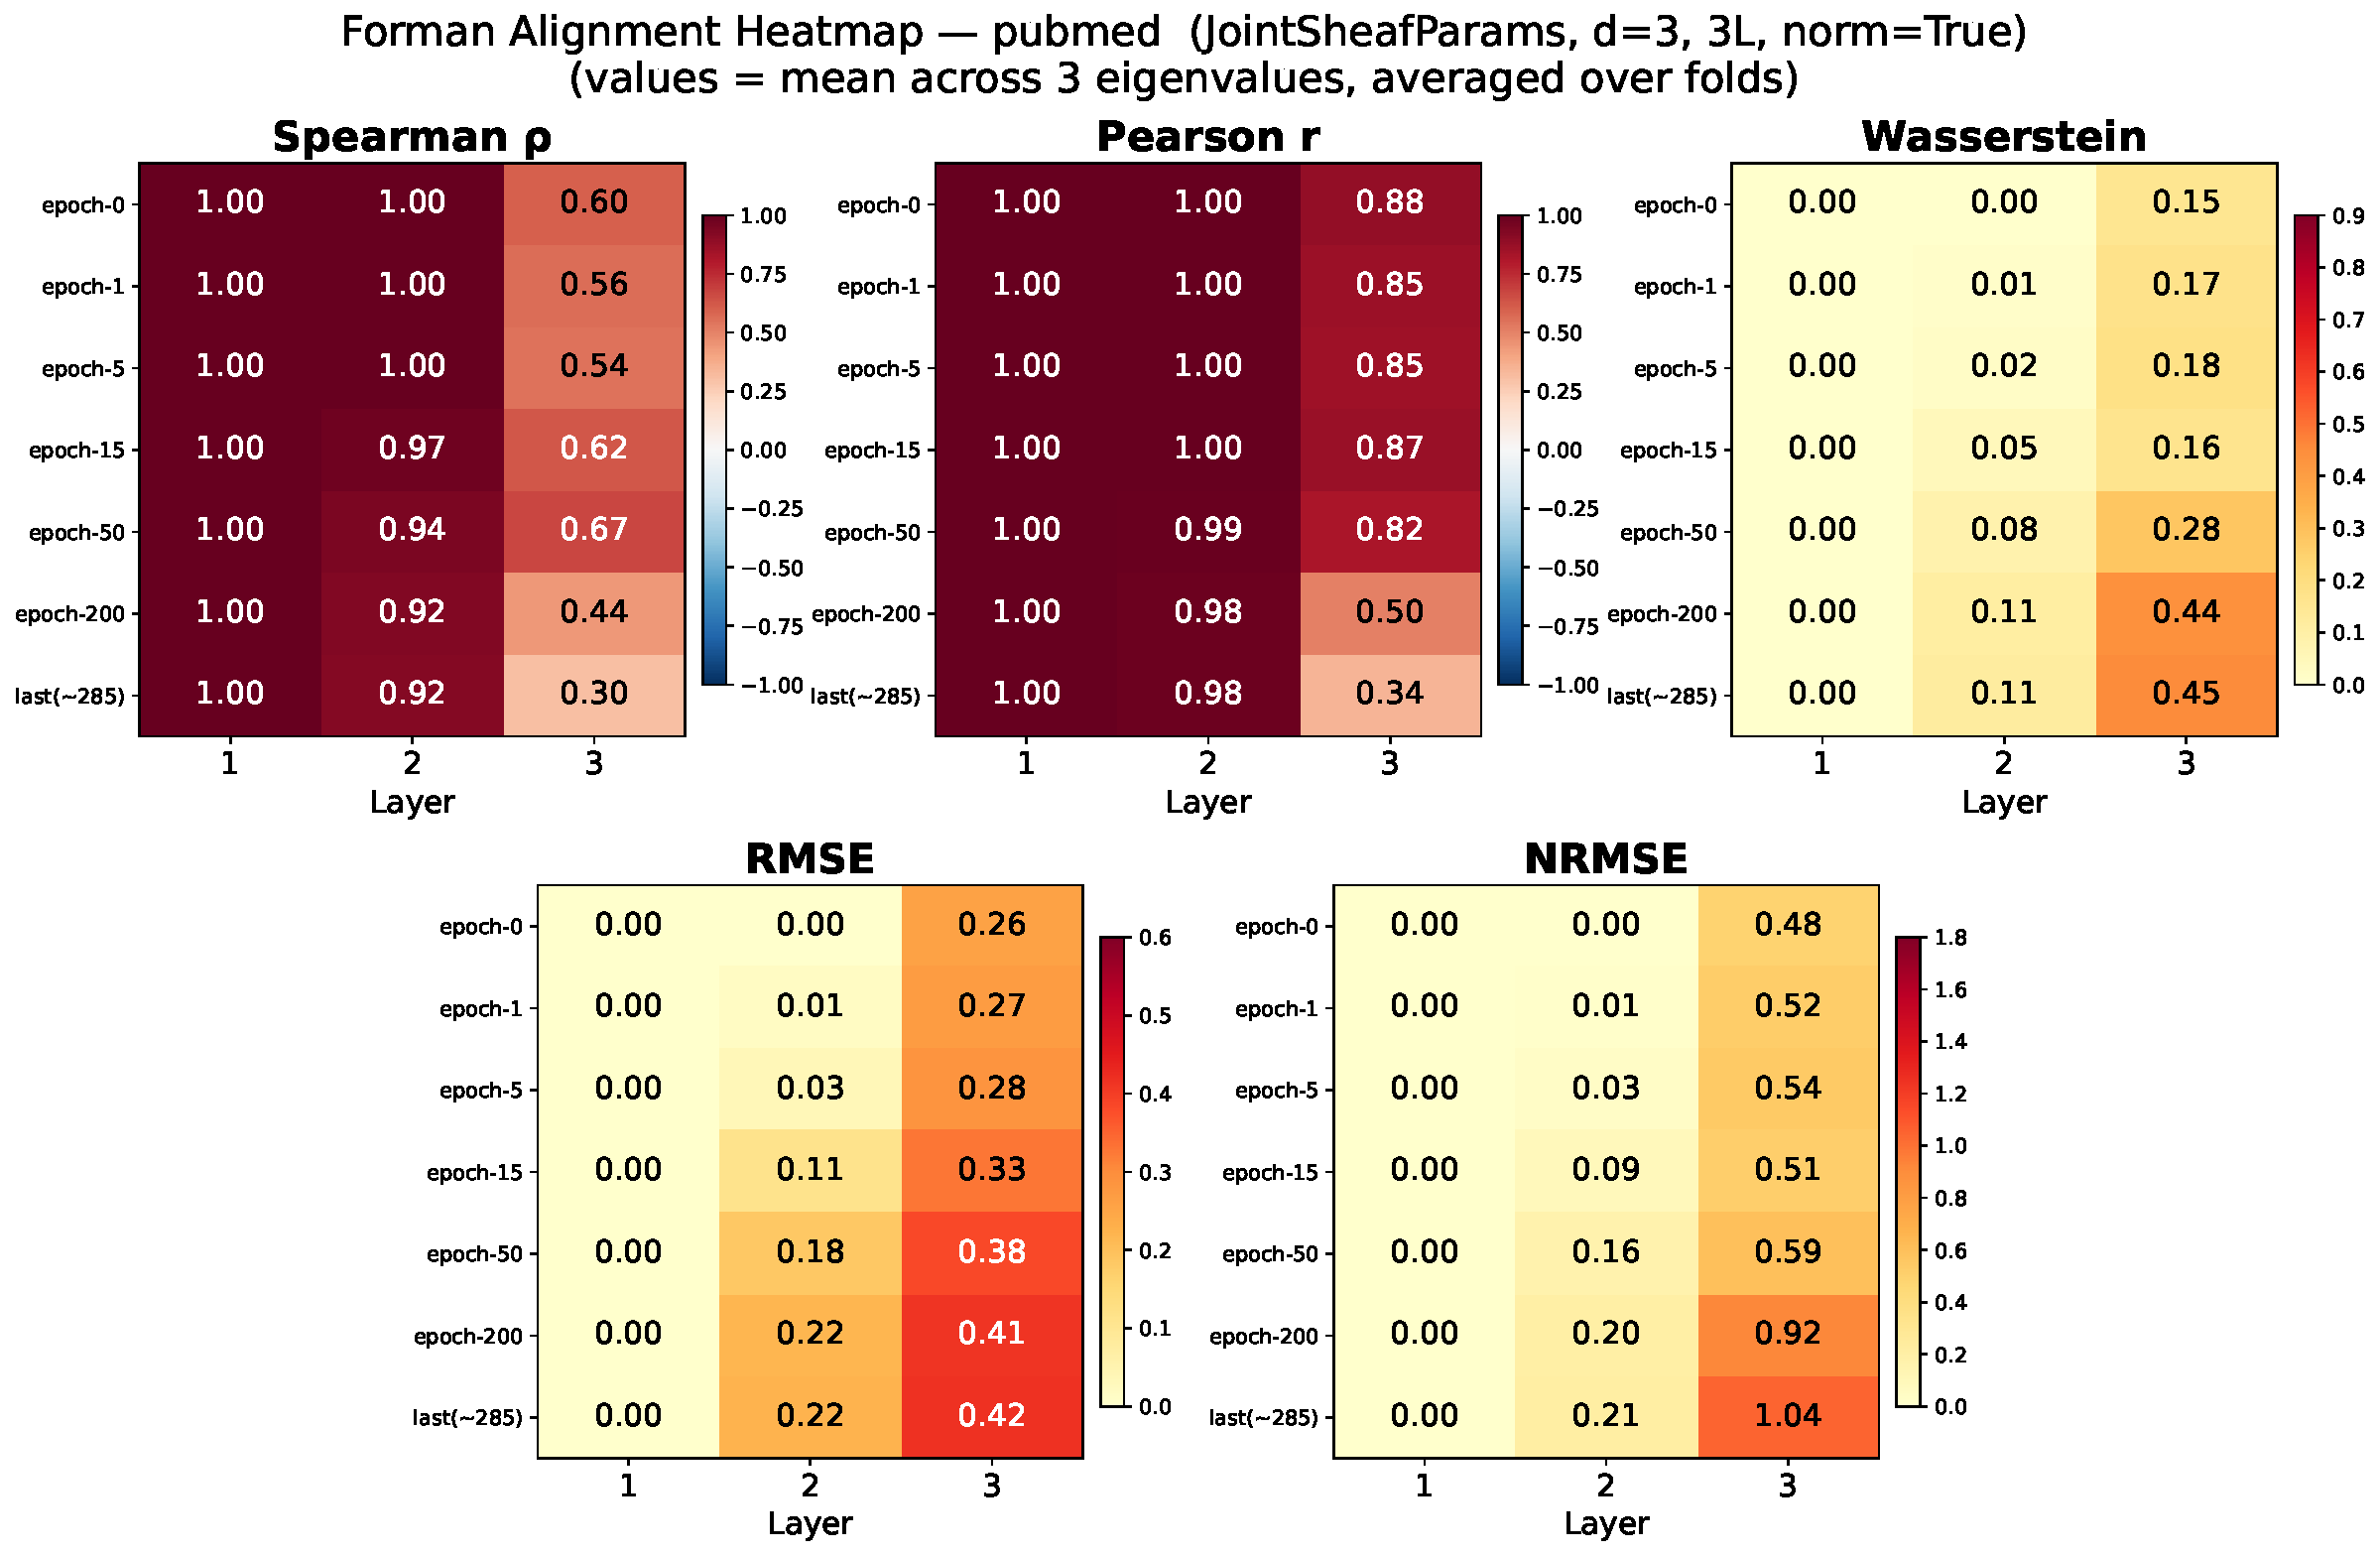
\includegraphics[width=\linewidth]{heatmaps/JointSheafParams/normalised_true/first_maps_identity/pubmed_JointSheafParams_d3_3L_Norm_True_first_maps_identity_heatmap.pdf}
\end{figure}
\end{frame}

\begin{frame}{Questions --- Joint, $d=2$, $L=4$, Norm=True, Identity}
\begin{figure}
    \centering
    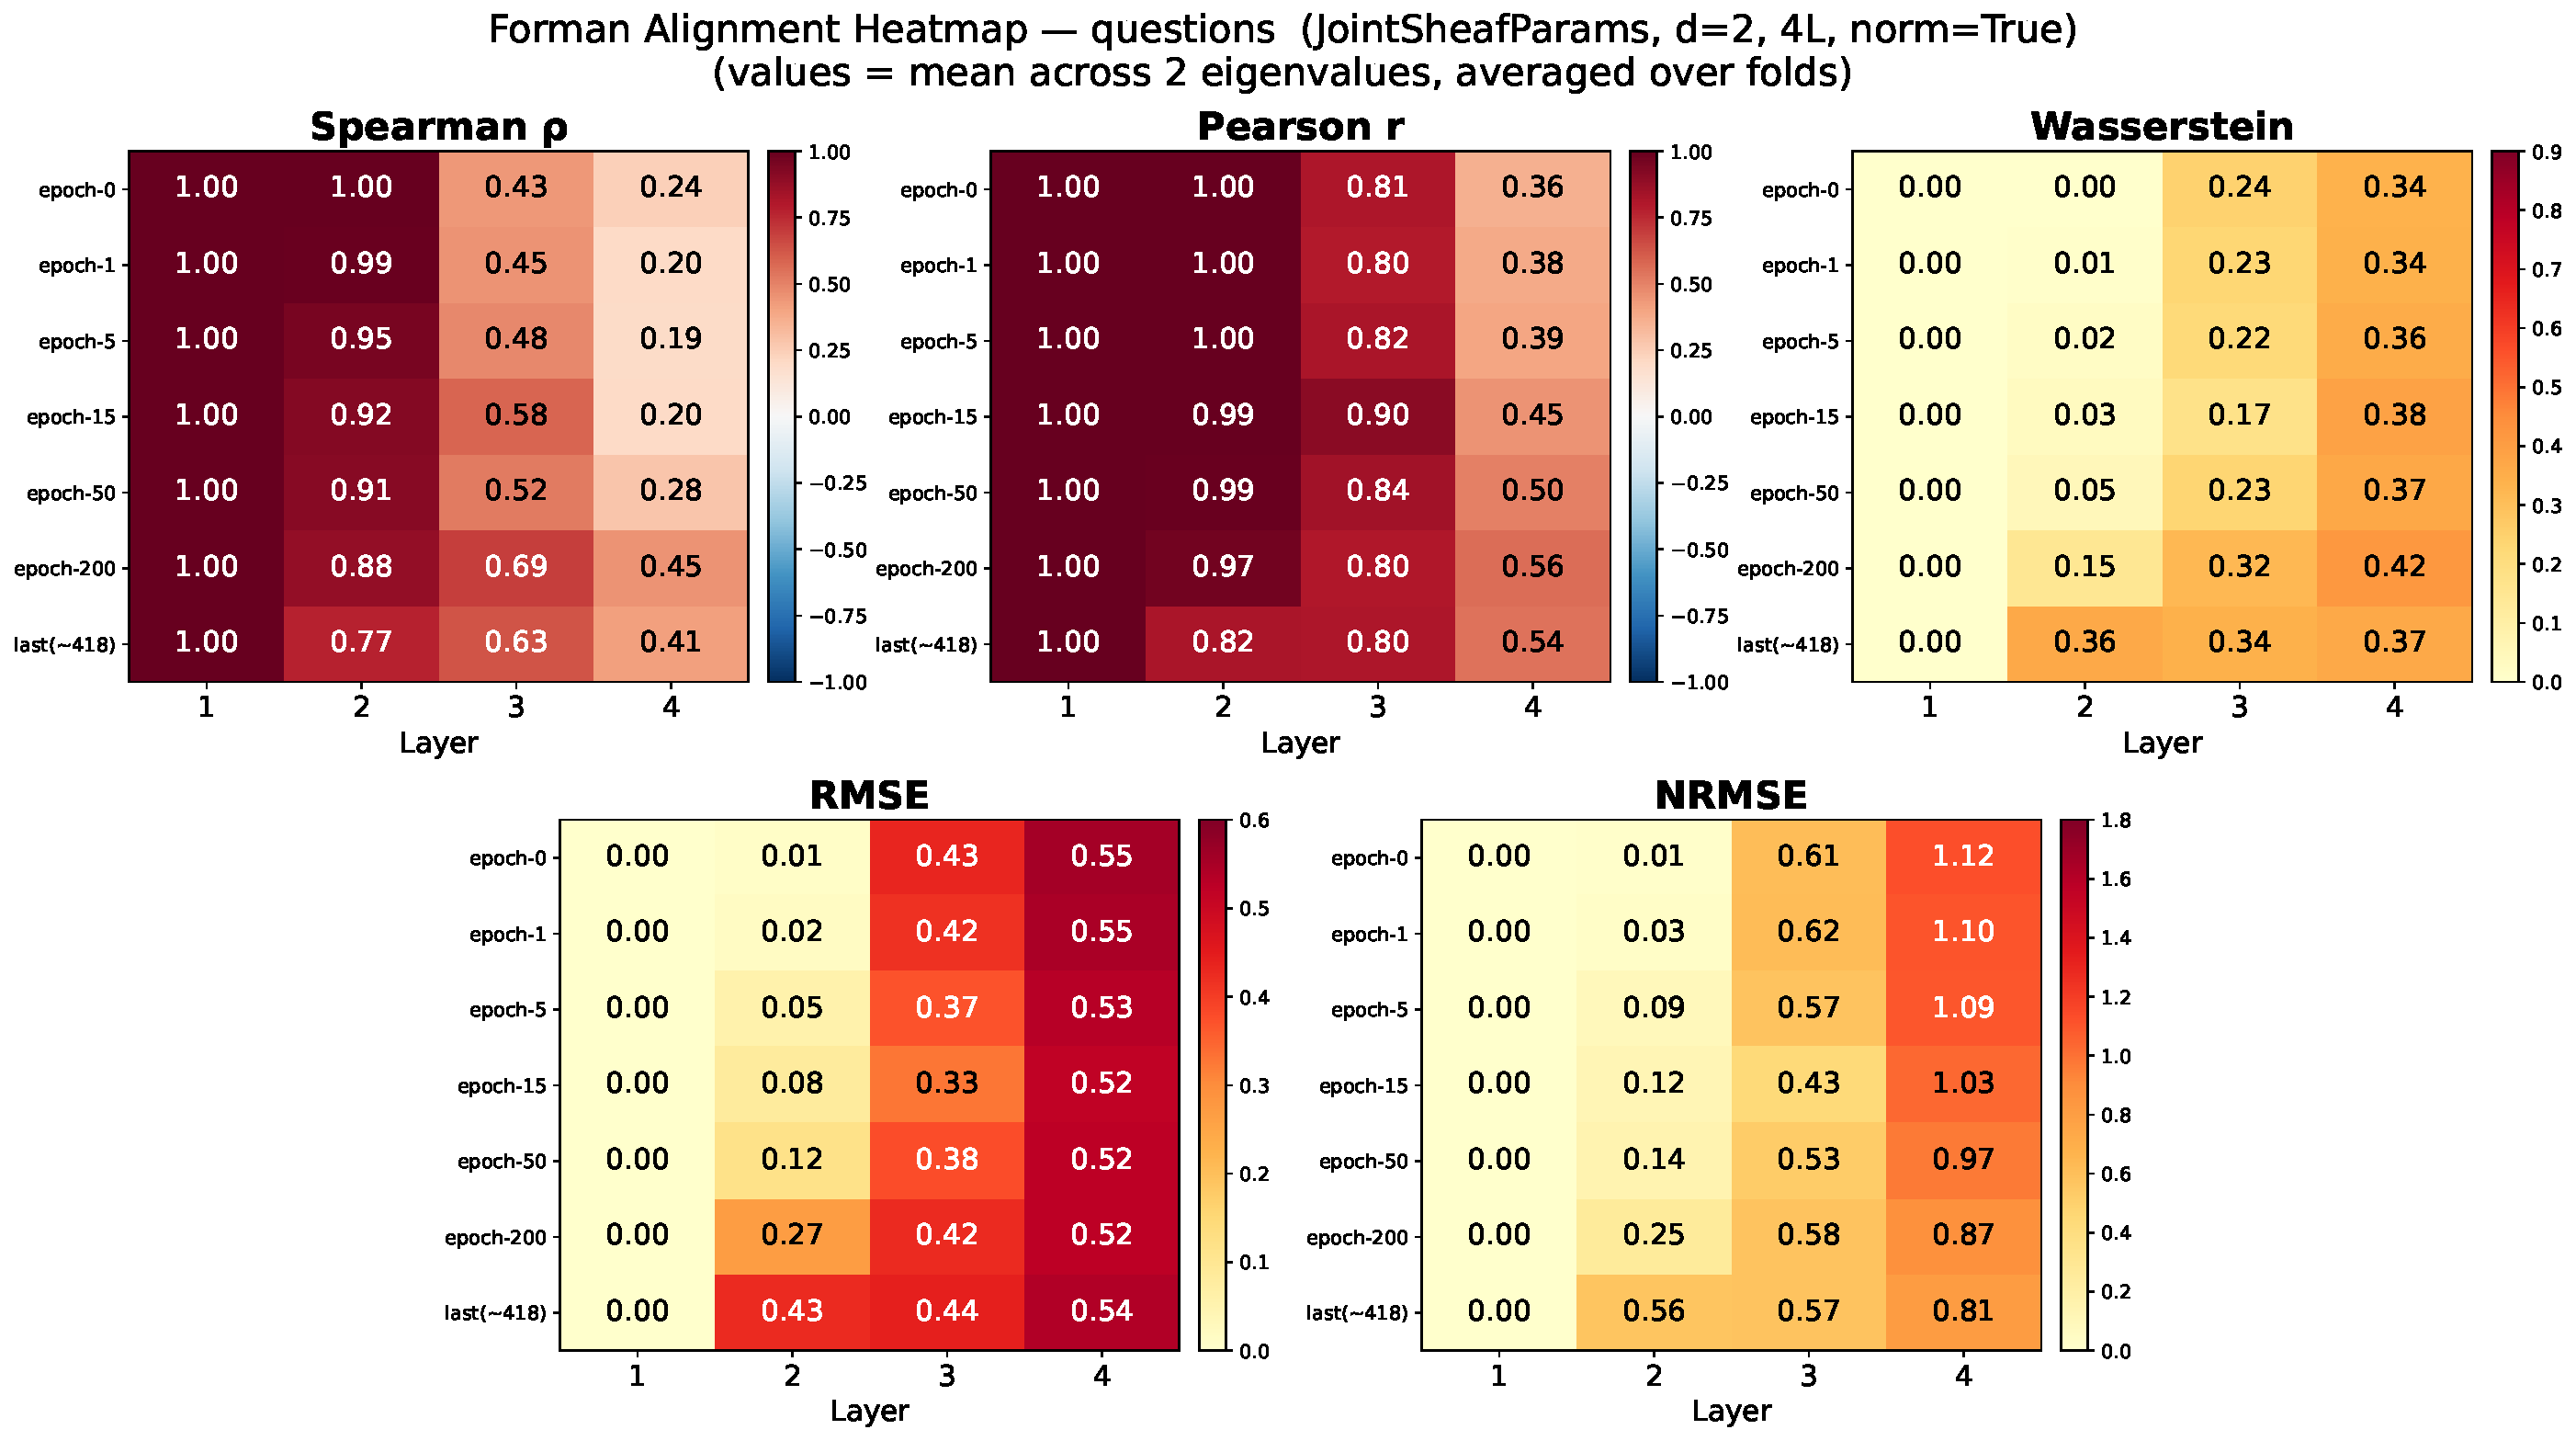
\includegraphics[width=\linewidth]{heatmaps/JointSheafParams/normalised_true/first_maps_identity/questions_JointSheafParams_d2_4L_Norm_True_first_maps_identity_heatmap.pdf}
\end{figure}
\end{frame}

\begin{frame}{Roman Empire --- Joint, $d=3$, $L=3$, Norm=True, Identity}
\begin{figure}
    \centering
    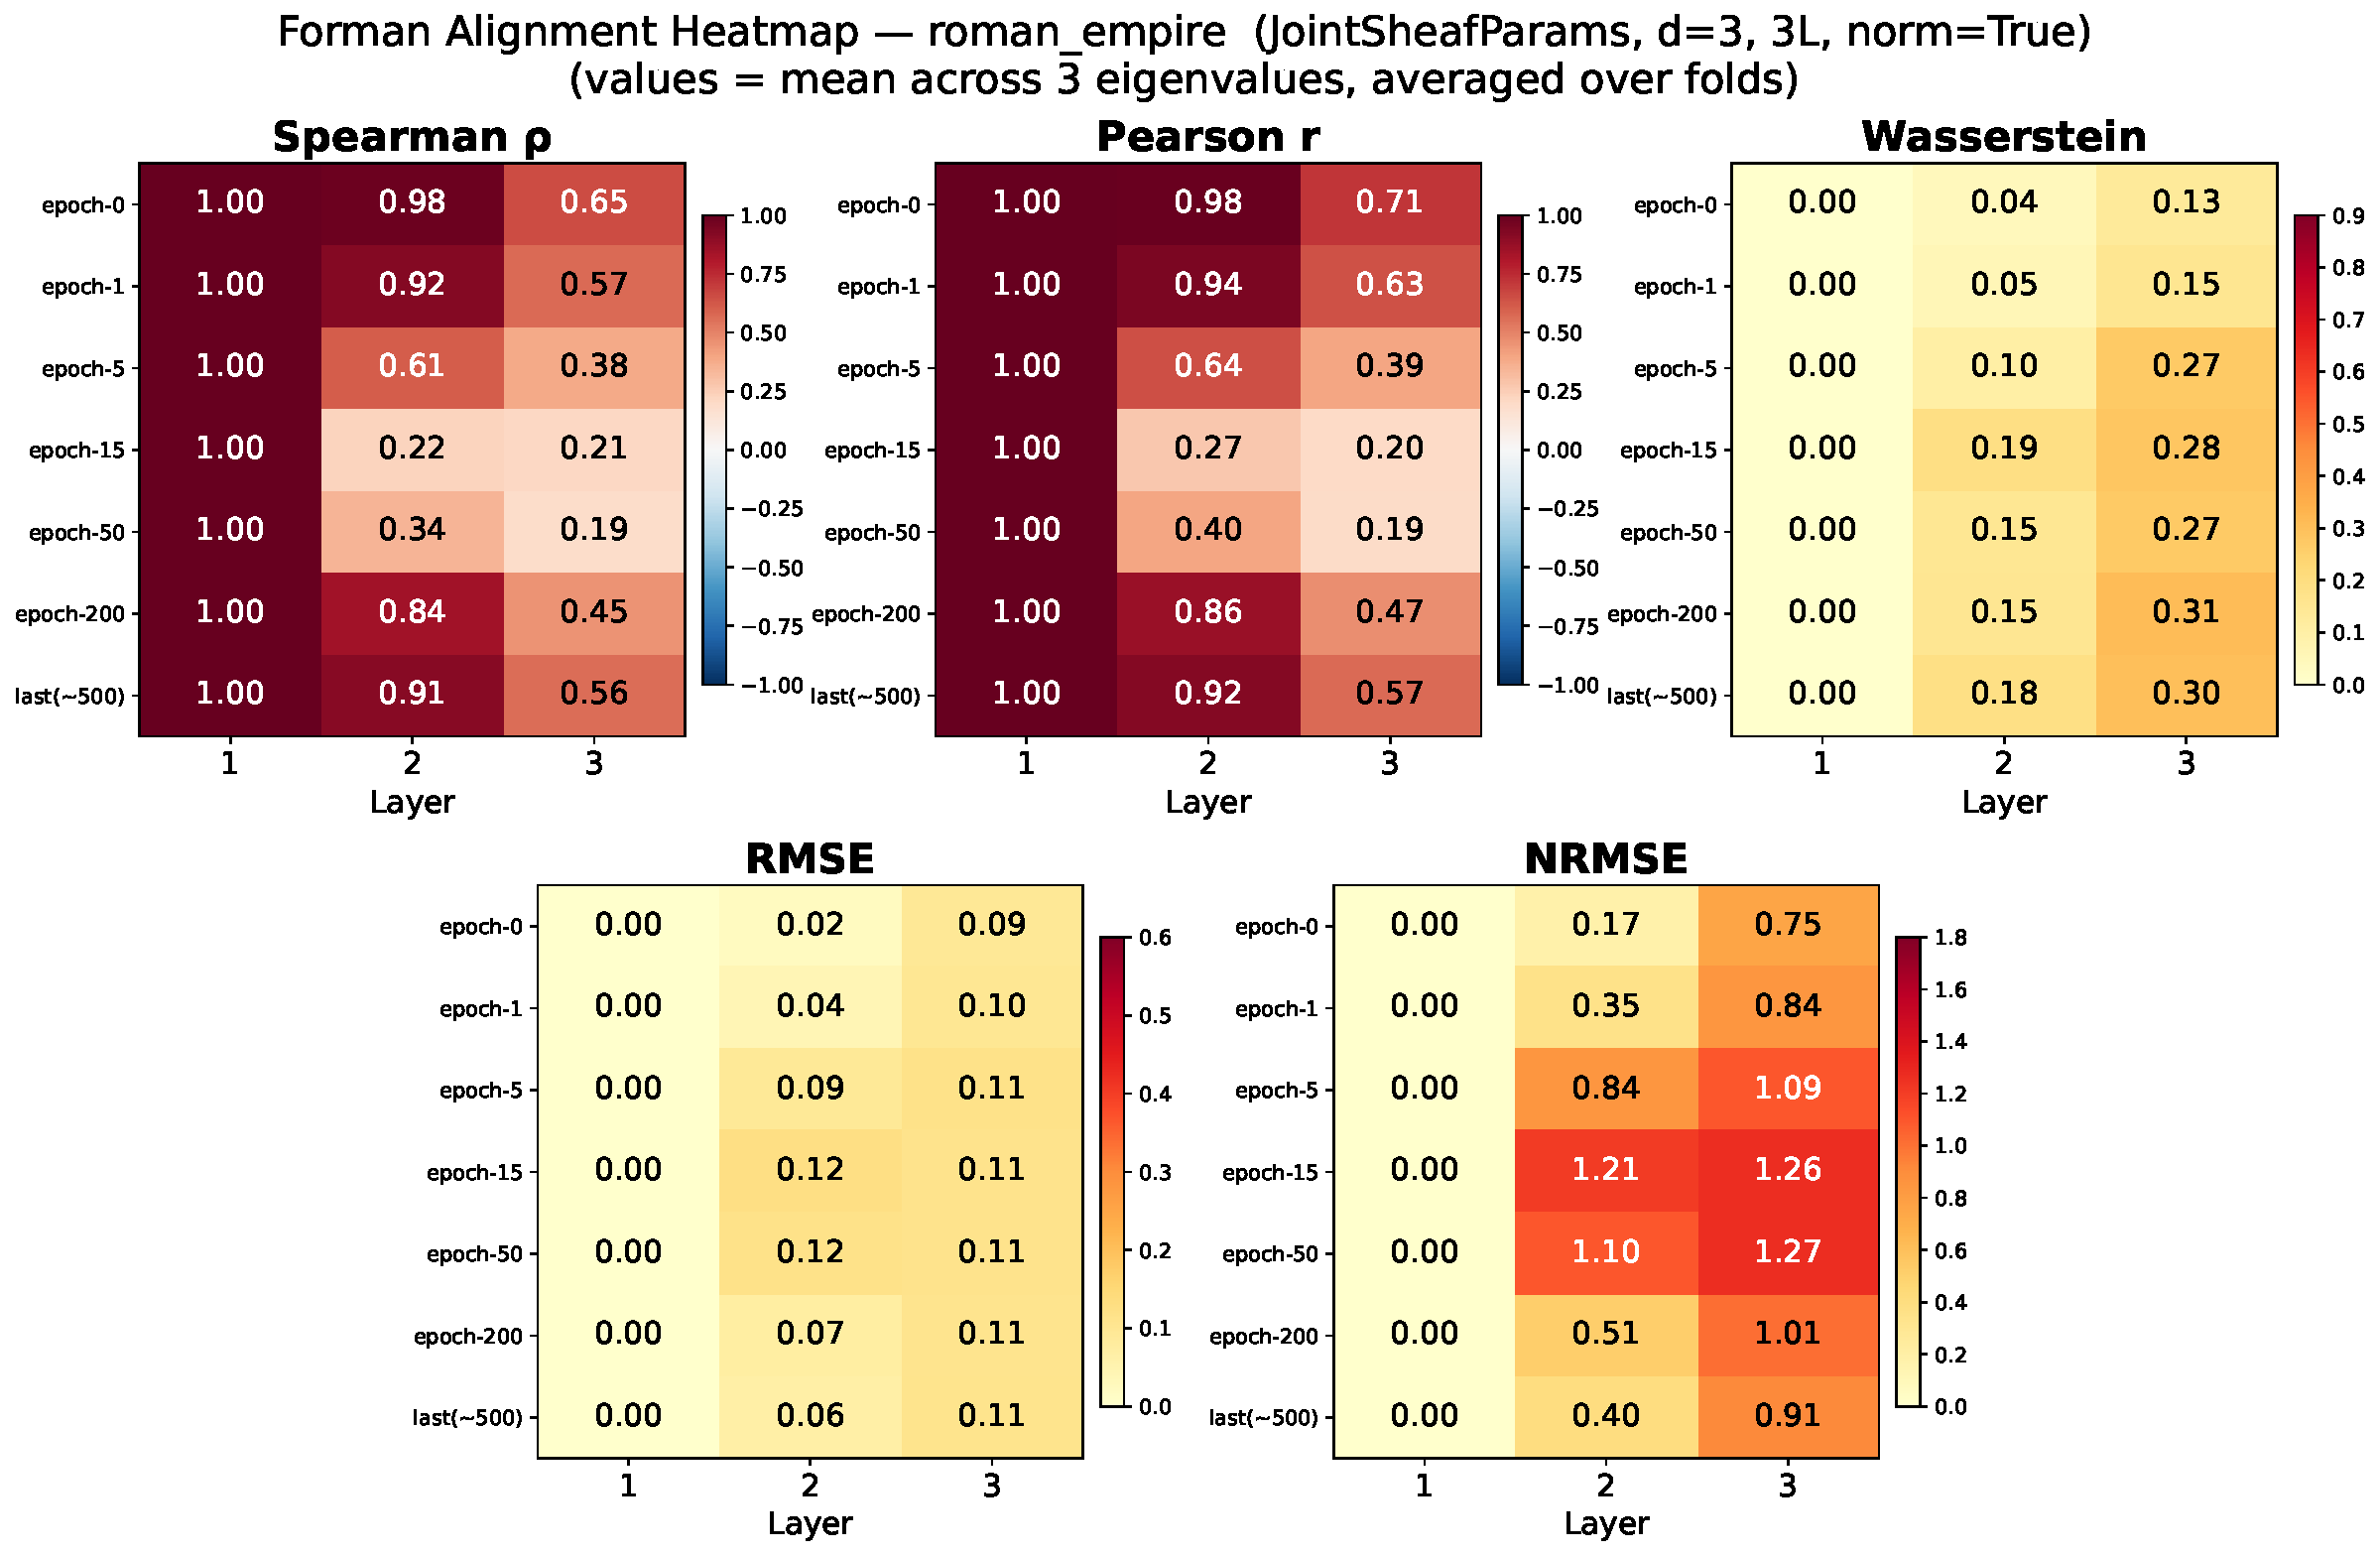
\includegraphics[width=\linewidth]{heatmaps/JointSheafParams/normalised_true/first_maps_identity/roman_empire_JointSheafParams_d3_3L_Norm_True_first_maps_identity_heatmap.pdf}
\end{figure}
\end{frame}

\begin{frame}{Wisconsin --- Joint, $d=2$, $L=2$, Norm=True, Identity}
\begin{figure}
    \centering
    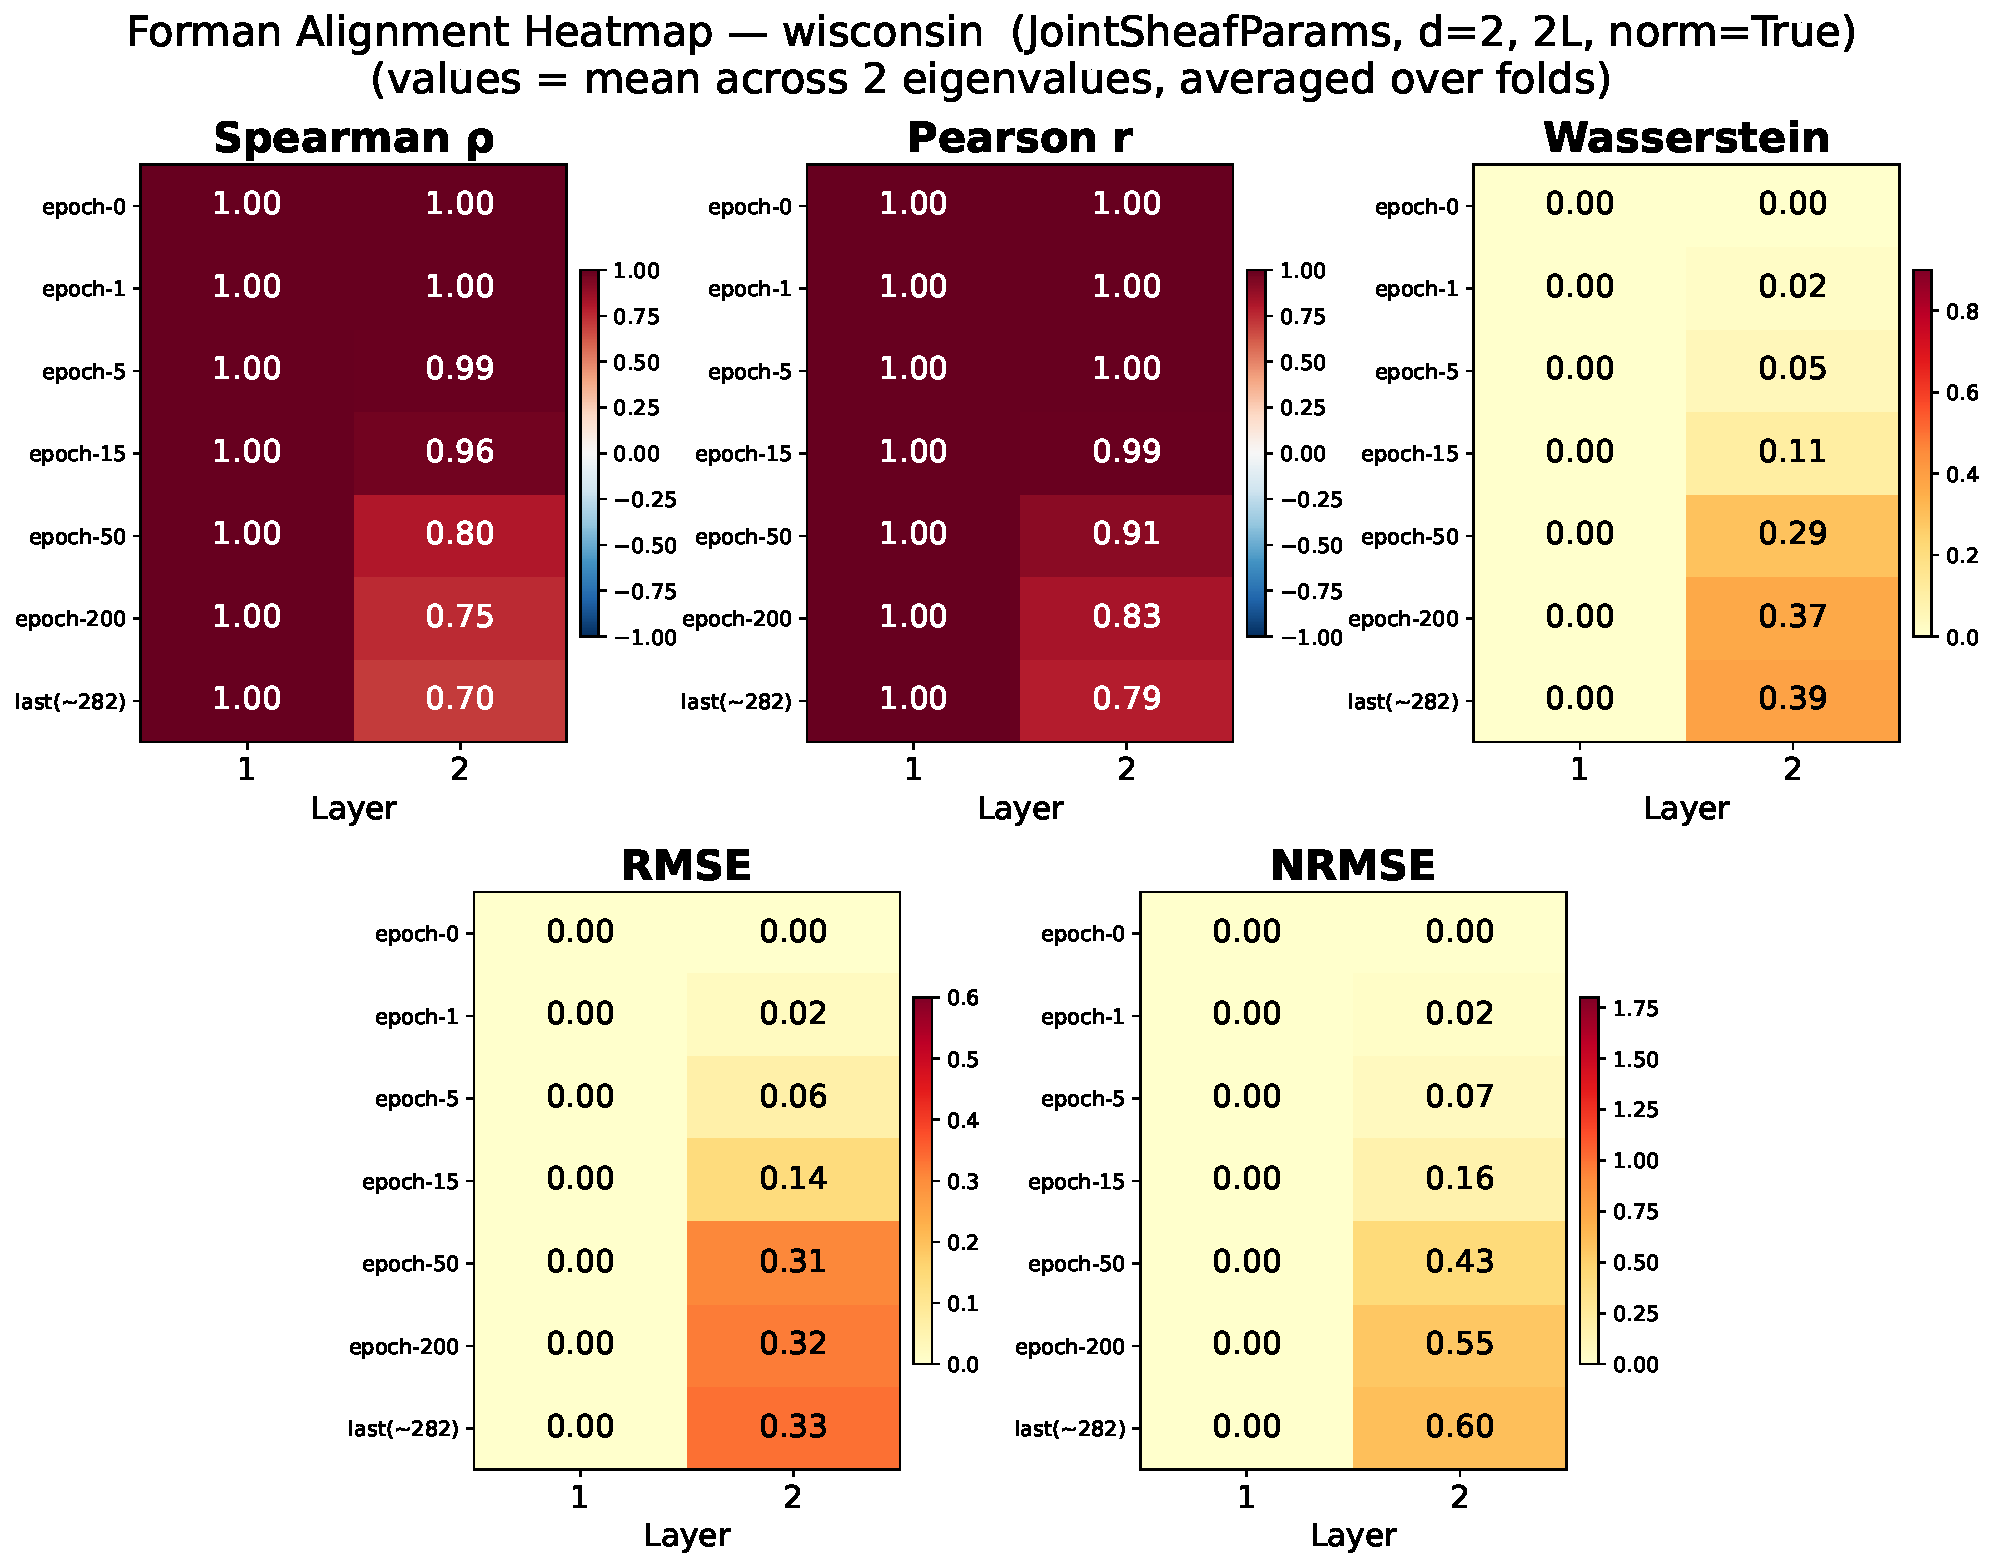
\includegraphics[width=\linewidth]{heatmaps/JointSheafParams/normalised_true/first_maps_identity/wisconsin_JointSheafParams_d2_2L_Norm_True_first_maps_identity_heatmap.pdf}
\end{figure}
\end{frame}

% ══════════════════════════════════════════════════════════════════════════════
%  SECTION 7 — GeneralSheaf: other Laplacian from Norm=False run
%              content = normalised, maps trained unnormalised
%              (--normalised=false --use_other  →  normalised_true_other/)
% ══════════════════════════════════════════════════════════════════════════════

\begin{frame}{}
\centering
\Huge\textbf{GeneralSheaf --- Other Laplacian}\\[6pt]
\Large Maps trained with \texttt{norm=False}\\
evaluated as normalised $\widetilde{\Delta}_{\mathcal{F}}$\\[4pt]
\normalsize (normalised metrics apply)
\end{frame}

\begin{frame}{Amazon Ratings --- Other $\widetilde{\Delta}_\mathcal{F}$ from Norm=False maps, $d=5$, $L=5$}
\begin{figure}
    \centering
    
\includegraphics[width=\linewidth]{heatmaps/GeneralSheaf/normalised_true_other/amazon_ratings_GeneralSheaf_d5_5L_Norm_False_heatmap.pdf}
\end{figure}
\end{frame}

\begin{frame}{Citeseer --- Other $\widetilde{\Delta}_\mathcal{F}$ from Norm=False maps, $d=5$, $L=4$}
\begin{figure}
    \centering
    
\includegraphics[width=\linewidth]{heatmaps/GeneralSheaf/normalised_true_other/citeseer_GeneralSheaf_d5_4L_Norm_False_heatmap.pdf}
\end{figure}
\end{frame}

\begin{frame}{Cora --- Other $\widetilde{\Delta}_\mathcal{F}$ from Norm=False maps, $d=5$, $L=3$}
\begin{figure}
    \centering
    
\includegraphics[width=\linewidth]{heatmaps/GeneralSheaf/normalised_true_other/cora_GeneralSheaf_d5_3L_Norm_False_heatmap.pdf}
\end{figure}
\end{frame}

\begin{frame}{Cornell --- Other $\widetilde{\Delta}_\mathcal{F}$ from Norm=False maps, $d=2$, $L=2$}
\begin{figure}
    \centering
    
\includegraphics[width=\linewidth]{heatmaps/GeneralSheaf/normalised_true_other/cornell_GeneralSheaf_d2_2L_Norm_False_heatmap.pdf}
\end{figure}
\end{frame}

\begin{frame}{Minesweeper --- Other $\widetilde{\Delta}_\mathcal{F}$ from Norm=False maps, $d=5$, $L=6$}
\begin{figure}
    \centering
    
\includegraphics[width=\linewidth]{heatmaps/GeneralSheaf/normalised_true_other/minesweeper_GeneralSheaf_d5_6L_Norm_False_heatmap.pdf}
\end{figure}
\end{frame}

\begin{frame}{Pubmed --- Other $\widetilde{\Delta}_\mathcal{F}$ from Norm=False maps, $d=5$, $L=4$}
\begin{figure}
    \centering
    
\includegraphics[width=\linewidth]{heatmaps/GeneralSheaf/normalised_true_other/pubmed_GeneralSheaf_d5_4L_Norm_False_heatmap.pdf}
\end{figure}
\end{frame}

\begin{frame}{Questions --- Other $\widetilde{\Delta}_\mathcal{F}$ from Norm=False maps, $d=5$, $L=4$}
\begin{figure}
    \centering
    
\includegraphics[width=\linewidth]{heatmaps/GeneralSheaf/normalised_true_other/questions_GeneralSheaf_d5_4L_Norm_False_heatmap.pdf}
\end{figure}
\end{frame}

\begin{frame}{Roman Empire --- Other $\widetilde{\Delta}_\mathcal{F}$ from Norm=False maps, $d=5$, $L=5$}
\begin{figure}
    \centering
    
\includegraphics[width=\linewidth]{heatmaps/GeneralSheaf/normalised_true_other/roman_empire_GeneralSheaf_d5_5L_Norm_False_heatmap.pdf}
\end{figure}
\end{frame}

\begin{frame}{Tolokers --- Other $\widetilde{\Delta}_\mathcal{F}$ from Norm=False maps, $d=3$, $L=4$}
\begin{figure}
    \centering
    
\includegraphics[width=\linewidth]{heatmaps/GeneralSheaf/normalised_true_other/tolokers_GeneralSheaf_d3_4L_Norm_False_heatmap.pdf}
\end{figure}
\end{frame}

\begin{frame}{Wisconsin --- Other $\widetilde{\Delta}_\mathcal{F}$ from Norm=False maps, $d=2$, $L=2$}
\begin{figure}
    \centering
    
\includegraphics[width=\linewidth]{heatmaps/GeneralSheaf/normalised_true_other/wisconsin_GeneralSheaf_d2_2L_Norm_False_heatmap.pdf}
\end{figure}
\end{frame}

% ══════════════════════════════════════════════════════════════════════════════
%  SECTION 8 — GeneralSheaf: other Laplacian from Norm=True run
%              content = unnormalised, maps trained normalised
%              (--normalised=true --use_other  →  normalised_false_other/)
% ══════════════════════════════════════════════════════════════════════════════

\begin{frame}{}
\centering
\Huge\textbf{GeneralSheaf --- Other Laplacian}\\[6pt]
\Large Maps trained with \texttt{norm=True}\\
evaluated as unnormalised $\Delta_{\mathcal{F}}$\\[4pt]
\normalsize (unnormalised metrics apply)
\end{frame}

\begin{frame}{Amazon Ratings --- Other $\Delta_\mathcal{F}$ from Norm=True maps, $d=5$, $L=5$}
\begin{figure}
    \centering
    
\includegraphics[width=\linewidth]{heatmaps/GeneralSheaf/normalised_false_other/amazon_ratings_GeneralSheaf_d5_5L_Norm_True_heatmap.pdf}
\end{figure}
\end{frame}

\begin{frame}{Citeseer --- Other $\Delta_\mathcal{F}$ from Norm=True maps, $d=5$, $L=4$}
\begin{figure}
    \centering
    
\includegraphics[width=\linewidth]{heatmaps/GeneralSheaf/normalised_false_other/citeseer_GeneralSheaf_d5_4L_Norm_True_heatmap.pdf}
\end{figure}
\end{frame}

\begin{frame}{Cora --- Other $\Delta_\mathcal{F}$ from Norm=True maps, $d=5$, $L=3$}
\begin{figure}
    \centering
    
\includegraphics[width=\linewidth]{heatmaps/GeneralSheaf/normalised_false_other/cora_GeneralSheaf_d5_3L_Norm_True_heatmap.pdf}
\end{figure}
\end{frame}

\begin{frame}{Cornell --- Other $\Delta_\mathcal{F}$ from Norm=True maps, $d=2$, $L=2$}
\begin{figure}
    \centering
    
\includegraphics[width=\linewidth]{heatmaps/GeneralSheaf/normalised_false_other/cornell_GeneralSheaf_d2_2L_Norm_True_heatmap.pdf}
\end{figure}
\end{frame}

\begin{frame}{Minesweeper --- Other $\Delta_\mathcal{F}$ from Norm=True maps, $d=5$, $L=6$}
\begin{figure}
    \centering
    
\includegraphics[width=\linewidth]{heatmaps/GeneralSheaf/normalised_false_other/minesweeper_GeneralSheaf_d5_6L_Norm_True_heatmap.pdf}
\end{figure}
\end{frame}

\begin{frame}{Pubmed --- Other $\Delta_\mathcal{F}$ from Norm=True maps, $d=5$, $L=4$}
\begin{figure}
    \centering
    
\includegraphics[width=\linewidth]{heatmaps/GeneralSheaf/normalised_false_other/pubmed_GeneralSheaf_d5_4L_Norm_True_heatmap.pdf}
\end{figure}
\end{frame}

\begin{frame}{Questions --- Other $\Delta_\mathcal{F}$ from Norm=True maps, $d=5$, $L=4$}
\begin{figure}
    \centering
    
\includegraphics[width=\linewidth]{heatmaps/GeneralSheaf/normalised_false_other/questions_GeneralSheaf_d5_4L_Norm_True_heatmap.pdf}
\end{figure}
\end{frame}

\begin{frame}{Roman Empire --- Other $\Delta_\mathcal{F}$ from Norm=True maps, $d=5$, $L=5$}
\begin{figure}
    \centering
    
\includegraphics[width=\linewidth]{heatmaps/GeneralSheaf/normalised_false_other/roman_empire_GeneralSheaf_d5_5L_Norm_True_heatmap.pdf}
\end{figure}
\end{frame}

\begin{frame}{Tolokers --- Other $\Delta_\mathcal{F}$ from Norm=True maps, $d=3$, $L=4$}
\begin{figure}
    \centering
    
\includegraphics[width=\linewidth]{heatmaps/GeneralSheaf/normalised_false_other/tolokers_GeneralSheaf_d3_4L_Norm_True_heatmap.pdf}
\end{figure}
\end{frame}

\begin{frame}{Wisconsin --- Other $\Delta_\mathcal{F}$ from Norm=True maps, $d=2$, $L=2$}
\begin{figure}
    \centering
    
\includegraphics[width=\linewidth]{heatmaps/GeneralSheaf/normalised_false_other/wisconsin_GeneralSheaf_d2_2L_Norm_True_heatmap.pdf}
\end{figure}
\end{frame}

\end{document}
